\documentclass[11pt]{article}
\usepackage[T1]{fontenc}
\usepackage[utf8]{inputenc}
\usepackage[a4paper,margin=23mm]{geometry}
\usepackage{amsmath,amssymb,amsthm,mathtools,longtable,graphicx}
\usepackage[colorlinks=true,linkcolor=blue,urlcolor=blue]{hyperref}
\hypersetup{pdftitle={The coupled Boussinesq control system with physical viscosity retained},pdfauthor={}}
\newtheorem{proposition}{Proposition}
\newtheorem{lemma}{Lemma}
\newtheorem{theorem}{Theorem}
\newcommand{\R}{\mathbb R}
\newcommand{\AB}{\mathrm{AB}}
\newcommand{\epsv}{\varepsilon_{\mathrm v}}
\newcommand{\kapth}{\kappa_{\mathrm{th}}}
\newcommand{\Gcal}{\mathcal G}
\newcommand{\dd}{\mathrm d}
\DeclareMathOperator{\tr}{tr}
\DeclareMathOperator{\sym}{sym}
% Load in the master document preamble, before \begin{document}.
\RequirePackage{amsmath,amssymb,amsthm,mathtools,mathrsfs}
\providecommand{\PDReal}{\mathbb R}
\providecommand{\PDTorus}{\mathbb T}
\providecommand{\PDd}{\mathrm d}
\providecommand{\PDthermal}{\kappa_{\rm th}}
\providecommand{\PDviscosity}{\nu_{\rm phys}}
\providecommand{\PDheat}{\mathcal H}
\providecommand{\PDmean}[1]{\langle #1\rangle}
\newtheorem{pdproposition}{Proposition}

\allowdisplaybreaks
\emergencystretch=2em
\title{The coupled Boussinesq control system with physical viscosity retained}
\author{}
\date{30 September 2026; finite-stage work begun 8 September 2026}
\begin{document}
\maketitle
\noindent This standalone calculation reconstructs the released
Alp\"oge--Buckmaster controls, proves the complete first controlled stage
in the original physical coordinates, and gives compact fields and
explicit smooth compactly supported forces realizing it with arbitrary
prescribed thermal diffusivity and physical viscosity. It then proves
a modified two-layer stage with an explicit positive equal-diffusion
range, both original temperature thresholds, the changing parent,
the second selected vorticity return, and a finite hold, together
with all original-profile compact fields and forces. The next complete
calculation follows the actual third growth and its full transition:
both parent temperatures evolve, the second vorticity revives during
transition, and the original third target is reached with an explicit
positive physical diffusion range. A compact continuation argument then
proves the complete third shooting family and selected third return on a
further definite positive equal-diffusion interval. Every phase, deformation, feedback,
scalar force, vector force and diffusion cost is retained. It also derives
the exact original third-steering map, proves an initial steering
interval with complete compact fields and forces, and completes the finite
third shooting return without assuming root uniqueness. The reader additionally derives
the evolving parent feedback, exact profile diffusion, and the
pressure-independent obstruction to retaining the released infinite
state with a smooth viscous force.  The exact two-parameter similarity
then transfers the complete finite third return to every spatial radius
at one fixed positive physical diffusion.  Its full force-jet weights
prove a raw-copy term obstruction and define the force-flat packet space
required by a corrected infinite accumulation.  It proves that complete
packets cannot be reset at consecutive scales because their endpoint curls
do not match, then derives the exact based-increment residual, every
space-time residual derivative, and the vector-and-matrix state interface
that a return-renormalization map must satisfy.  The infinite viscous
singularity construction remains open. Original $A_0,\lambda_0$, spatial scaling
$\mu$, and the paper's time-scaling $\nu=\sqrt{A_0}$ are retained.
The appendix sections use explicitly declared alternative notation for
physical viscosity to avoid confusing it with this $\nu$.

\medskip
\noindent Primary source: Levent Alp\"oge and Tristan Buckmaster,
\emph{Blowup for the Boussinesq equations with smooth forcing},
76-page released PDF,
\url{https://cims.nyu.edu/~tristanb/boussinesq.pdf}.
The exact downloaded edition is identified by the SHA-256 in
\texttt{checks/replay\_exact.json}. Printed-page and equation
citations accompany the calculations. Source infinite existence
results are attributed as such; the analytic finite-stage and
operator proofs are written here in full.
\setcounter{tocdepth}{1}
\tableofcontents
\clearpage
\section{Physical coordinates and exact finite viscous realization}
\label{sec:physical}
We use the orientation
\[
 x=(x_1,x_2)\in\mathbb R^2,\quad e_2=(0,1),\quad
 J=\begin{pmatrix}0&-1\\1&0\end{pmatrix},\quad
 \nabla^\perp=J\nabla,\quad \operatorname{curl}u=\partial_1u_2-\partial_2u_1.
\]
The physical equations throughout this note are
\begin{align}
 \theta_t+u\cdot\nabla\theta&=\kappa\Delta\theta+f_\theta,
 \label{eq:physicaltheta}\\
 u_t+(u\cdot\nabla)u+\nabla p&=\varepsilon\Delta u+\theta e_2+f_u,
 \qquad \operatorname{div}u=0.\label{eq:physicalu}
\end{align}
Here $\kappa,\varepsilon\geq0$ are respectively thermal diffusivity and
physical viscosity. In particular $\varepsilon$ is not the source's
time-scaling parameter $\nu$ and is not its schedule error tolerance.
The datum is retained exactly:
\[
 A_0\geq1,\quad \lambda_0=\lceil\sqrt{A_0}/2\rceil,
 \qquad \theta_{\rm in}(x)=-\frac{A_0}{\lambda_0}
 \sin(\lambda_0x_2)\chi_0(x),\qquad u_{\rm in}(x)=0.
\]
The original radial cutoff $\chi_0\in C_c^\infty(B_{R_0})$, $R_0>2$,
equals one on $B_2$ and lies in $[0,1]$. Define
\[
 \mu=\lambda_0,\qquad \nu=\sqrt{A_0},\qquad (X,T)=(\mu x,\nu t).
\]
These are explicit maps between the source coordinates and the physical
coordinates, rather than replacements of $A_0$ or $\lambda_0$ by one.
For source fields decorated with a tilde their pullback is
\begin{align}
 \theta(x,t)&=\frac{\nu^2}{\mu}\widetilde\theta(\mu x,\nu t),&
 u(x,t)&=\frac\nu\mu\widetilde u(\mu x,\nu t),\notag\\
 p(x,t)&=\frac{\nu^2}{\mu^2}\widetilde p(\mu x,\nu t),&
 \psi(x,t)&=\frac\nu{\mu^2}\widetilde\psi(\mu x,\nu t).
 \label{eq:physicalmap}
\end{align}
Their forces pull back with factors $\nu^3/\mu$ and $\nu^2/\mu$,
respectively. Their source diffusion coefficients must be
\begin{equation}
 \widetilde\kappa=\frac{\mu^2}{\nu}\kappa,
 \qquad \widetilde\varepsilon=\frac{\mu^2}{\nu}\varepsilon.
 \label{eq:viscscale}
\end{equation}
Indeed each term on the left of the scalar equation acquires
$\nu^3/\mu$, whereas $\kappa\Delta_x\theta$ acquires
$\kappa\nu^2\mu$. Each momentum and buoyancy term acquires
$\nu^2/\mu$, whereas $\varepsilon\Delta_xu$ acquires
$\varepsilon\nu\mu$. Division gives exactly \eqref{eq:viscscale}.
Also $\nabla_x^\perp\psi=u$, $\Delta_x\psi=\nu\widetilde\omega$,
and $\operatorname{div}_xu=\nu\operatorname{div}_X\widetilde u$.
The inverse map substitutes $(x,t)=(X/\mu,T/\nu)$ and reciprocates
the displayed factors, proving a bijection for corresponding forces,
coefficients, and initial values. The cutoff is
$\widetilde\chi_0(X)=\chi_0(X/\mu)$, so the pulled-back initial
temperature is exactly the displayed $\theta_{\rm in}$.
These computations extend source Lemma 1.2, equations (1.6)--(1.7),
pp.~6--7, by retaining both diffusion coefficients.

\subsection{The released profile, the initial interpolation, and the base}
Fix $0<s_0<1$ and an even smooth cutoff $\chi$ supported in
$(-\pi,\pi)$, equal to one on $[-s_0,s_0]$. On $[-\pi,\pi]$ put
\[
 F(s)=\sin s+\chi(s)(s-\sin s)
\]
and extend periodically. Let
\[
 P(s)=\int_0^sF(r)\,dr-
 \frac1{2\pi}\int_{-\pi}^{\pi}\int_0^yF(r)\,dr\,dy.
\]
Oddness and zero period integral of $F$ show that $P$ is even,
periodic, has zero mean, and $P'=F$. Near zero, $F(s)=s$ and
$P(s)=P(0)+s^2/2$. No sinusoidal identity is substituted for this profile.
Take a smooth nondecreasing step $\eta$ that is zero for $t\leq0$
and one for $t\geq1$. Every derivative of positive order vanishes
at its endpoints: smoothness and its constant extension prove this.

Choose $R_H>R_0+1$ and radial $H\in C_c^\infty(B_{R_H})$ equal to
$|x|^2/2$ on $B_{R_0+1}$. Let $\alpha=0$ on $[0,1/\nu]$ and
$e_0=R_\alpha e_2$. Define
\begin{align}
 \theta_0&=-\frac{A_0}{\mu}F(\mu e_0\cdot x)\chi_0(x),&
 \theta_{\rm ref}&=-\frac{A_0}{\mu}F(\mu x_2)\chi_0(x),\notag\\
 \theta_b&=\theta_0+(1-\eta(\nu t))
          (\theta_{\rm in}-\theta_{\rm ref}),&
 \psi_b&=\dot\alpha H,\qquad u_b=\dot\alpha J\nabla H.
 \label{eq:basephysical}
\end{align}
For $t\leq1/\nu$, $u_b=0$ and
$\partial_t\theta_b=\nu\eta'(\nu t)(\theta_{\rm ref}-\theta_{\rm in})$.
For later times, $u_b=\dot\alpha Jx$ on the support of $\theta_0$.
Since $\dot e_0=\dot\alpha Je_0$,
\[
 (\partial_t+\dot\alpha Jx\cdot\nabla)(\mu e_0\cdot x)
 =\mu\dot\alpha(Je_0\cdot x+e_0\cdot Jx)=0.
\]
Radiality gives $Jx\cdot\nabla\chi_0=0$. Therefore the exact
zero-pressure base forces are
\begin{align}
 f^0_{\theta,b}&=\nu\eta'(\nu t)(\theta_{\rm ref}-\theta_{\rm in}),\notag\\
 f^0_{u,b}&=\ddot\alpha J\nabla H+
 \dot\alpha^2(J\nabla H\cdot\nabla)(J\nabla H)-\theta_b e_2.
 \label{eq:baseforces}
\end{align}
On $|\mu e_0\cdot x|<s_0$, $|x|<2$, and $t\geq1/\nu$, the
base has the exact values
\[
 \theta_b=-A_0e_0\cdot x,\quad u_b=\dot\alpha Jx,
 \quad G_b=-A_0e_0,\quad D_b=\dot\alpha J.
\]
This is source (4.9)--(4.10), pp.~38--39, in the original coordinates.

\subsection{A compact realization of the complete first controlled stage}
Use the first-stage coefficients constructed and proved below, with
physical frequency $K_1=\mu\lambda_1$, phase $\zeta=R_\alpha e(s_*)$,
$|\zeta|=1$, and signed amplitudes $\Theta,\Omega$ satisfying
\begin{equation}
 \dot\Theta=-\frac{J\zeta\cdot G_b}{K_1}\Omega,
 \qquad \dot\Omega=K_1\zeta_1\Theta.
 \label{eq:firstphysicalpair}
\end{equation}
Here $e(\phi)=(\sin\phi,\cos\phi)$ and
$J\zeta\cdot G_b=-A_0\sin s_*$, a rotationally invariant scalar.
Choose $C_\ell\geq4$, set $\ell=s_0/(C_\ell\mu)$, and take
radial $f\in C_c^\infty(B_1)$ equal to one on $B_{1/2}$.
Put
\[
 g(x)=f(x/\ell),\quad s=K_1\zeta\cdot x,\quad
 w=\eta(\Gamma(t-1/\nu)),\quad \Gamma=\nu\sin s_*,
 \quad T=w\Theta,\quad Q=\frac{w\Omega}{K_1^2}.
\]
Although $g$ is written in laboratory coordinates, it is exactly
the paper's material envelope: $M=R_\alpha$, so
$f(M^{-1}x/\ell)=f(x/\ell)$ by radiality. Set
\begin{align}
 V&=TF(s)g,& \Psi&=QP(s)g,\notag\\
 v&=Q\{K_1J\zeta F(s)g+P(s)J\nabla g\},&
 \theta&=\theta_b+V,\quad u=u_b+v,\quad p=0.
 \label{eq:compactfields}
\end{align}
The new fields are extended by zero before $t=1/\nu$. They are
smooth across that time because $w$ is flat there. Their support
is in $B_\ell\subset B_{s_0/\mu}\cap B_2$, where the base is
affine for every angle. The phase and envelope satisfy
\[
 (\partial_t+D_bx\cdot\nabla)s=0,
 \qquad (\partial_t+D_bx\cdot\nabla)g=0.
\]
For the phase this follows from
$\dot\zeta=\dot\alpha J\zeta=-D_b^T\zeta$; for the
envelope it follows from radiality.

Write $\partial_\perp g=J\zeta\cdot\nabla g$. Direct expansion
gives the following complete added forces at zero diffusion:
\begin{align}
 E^0_\theta={}&\dot w\Theta Fg+
 QP(J\nabla g\cdot G_b)
 +K_1QT(F^2-PF')g\partial_\perp g,
 \label{eq:compactscalarforce}\\
 E^0_u={}&2D_bv+
 \dot Q\{K_1J\zeta Fg+PJ\nabla g\}
 +(v\cdot\nabla)v-TFg e_2.
 \label{eq:compactvectorforce}
\end{align}
Every function of $s$ in these equations is evaluated at the phase
in \eqref{eq:compactfields}. The vector derivative in the last formula
can, equivalently, be evaluated by the explicitly specified matrix
\[
 \nabla v=QJ\left[
 K_1^2\zeta\otimes\zeta F'g
 +K_1F(\zeta\otimes\nabla g+\nabla g\otimes\zeta)
 +P\nabla^2g\right],\qquad
 (v\cdot\nabla)v=(\nabla v)v.
\]
Thus \eqref{eq:compactvectorforce} is a direct component formula,
without solving a pressure equation or an inverse-curl problem.

Here is a proof of both residual identities. Since $J\zeta\cdot\zeta=0$,
\[
 v\cdot\nabla V=K_1QT(F^2-PF')g(J\zeta\cdot\nabla g).
\]
Also $v\cdot G_b=QK_1(J\zeta\cdot G_b)Fg+
 QP(J\nabla g\cdot G_b)$ and the material derivative of $V$ is
$\dot T Fg$. Equation \eqref{eq:firstphysicalpair} implies
$\dot T+QK_1J\zeta\cdot G_b=\dot w\Theta$, proving
\eqref{eq:compactscalarforce}. For any trace-free matrix $D$,
direct multiplication proves $DJ+JD^T=0$. Consequently
\[
 (\partial_t+Dx\cdot\nabla)J\nabla\Psi
 =D J\nabla\Psi+J\nabla[(\partial_t+Dx\cdot\nabla)\Psi].
\]
The material derivative of $\Psi$ is $\dot QPg$, and
$(v\cdot\nabla)u_b=D_bv$ on the new support. Adding these two
terms, the self-advection, and the negative buoyancy increment
proves \eqref{eq:compactvectorforce}. Away from the new support
every increment vanishes, so this verification is global.

For every prescribed $\kappa,\varepsilon\geq0$ the \emph{same}
controlled fields now solve \eqref{eq:physicaltheta}--\eqref{eq:physicalu}
with the explicit forces
\begin{align}
 f_\theta^{\kappa,\varepsilon}
 &=f^0_{\theta,b}+E^0_\theta-\kappa\Delta\theta_b-\kappa\Delta V,
 \label{eq:exactviscforce}\\
 f_u^{\kappa,\varepsilon}
 &=f^0_{u,b}+E^0_u-\varepsilon\Delta u_b-\varepsilon\Delta v.
 \label{eq:exactviscu}
\end{align}
Indeed substituting these right-hand sides cancels the displayed
diffusion terms exactly and leaves the two residual identities
already proved. This proves a concrete finite controlled viscous
stage, for arbitrary physical coefficients, retaining the paper's
actual profile and motion. Its costs are calculated next; no
claim that these are small or uniform over infinitely many stages
is part of this construction.

All fields and forces are supported in the fixed spatial ball
$B_{R_H}$. They are smooth on the complete closed finite interval,
including interpolation, activation, growth, transition, steering,
and any specified finite holding duration. The pressure $p=0$
satisfies $p(0,t)=0$. Since $\psi_b+\Psi$ is compactly supported,
$u=J\nabla(\psi_b+\Psi)$ is divergence free and has finite
spatial energy. It also has exactly the Biot--Savart relation
$u=K\omega$: if $N=(2\pi)^{-1}\log|x|$, integration by parts
against the compact streamfunction gives
$N*\Delta(\psi_b+\Psi)=(\Delta N)*(\psi_b+\Psi)=\psi_b+\Psi$;
applying $J\nabla$ proves the assertion in distributions and hence
for these smooth fields. Odd $F$, even $P$, and radial cutoffs
give odd $\theta,u,f_\theta,f_u$ and even $\omega$.
The finite-slab forces can also be specified with compact temporal
support. Extend the state by its stationary initial values to the
left and its stationary held values to the right; flatness of the
interpolation and the selected pulse proves smoothness of these
extensions. For any fixed $\tau_{\rm ext}>0$, multiply the
resulting force formulas by
\[
 \eta(1+t/\tau_{\rm ext})
 \eta(1+(T_f-t)/\tau_{\rm ext}).
\]
Here $T_f$ denotes the finite final time of the prescribed hold.
This multiplier is one on $[0,T_f]$ and zero outside
$(-\tau_{\rm ext},T_f+\tau_{\rm ext})$. Thus the same solution
on its specified slab has forces in $C_c^\infty(\mathbb R^2\times
\mathbb R)$, with explicitly specified spatial and temporal support.

On the smaller open set
\[
 |x|<\ell/2,\qquad |K_1\zeta\cdot x|<s_0,
\]
the exact fields are
\begin{equation}
 \theta=(-A_0e_0+wK_1\Theta\zeta)\cdot x,
 \quad u=(\dot\alpha J+w\Omega J\zeta\otimes\zeta)x.
 \label{eq:actualparentcore}
\end{equation}
Their Laplacians vanish there, and so do the additional diffusive
forces \emph{and all their spatial derivatives} there. Therefore
the evolving parent background for a next layer inside this open
set is exactly the coupled gradient and shear in
\eqref{eq:actualparentcore}, with the actual time-dependent
$\Theta,\Omega,\alpha,w$. It has not been replaced by prescribed
unchanging $D,G$. The finite-stage force supplies the compensating
diffusion outside this affine region.

\subsection{Every spatial diffusion cost, including the cutoff terms}
Put $k=K_1\zeta$, so $|k|=K_1$. Direct differentiation gives
\begin{align}
 \Delta V={}&T\{K_1^2F''g+2F'k\cdot\nabla g+F\Delta g\},
 \label{eq:lapV}\\
 \Delta v={}&QJ\{K_1^2kF''g+K_1^2F'\nabla g
 +2F'k(k\cdot\nabla g)\notag\\
 &\hspace{26mm}+2F\nabla(k\cdot\nabla g)
 +Fk\Delta g+P\nabla\Delta g\}.
 \label{eq:lapv}
\end{align}
For the second formula first differentiate
$\Delta\Psi=Q\{K_1^2F'g+2F k\cdot\nabla g+P\Delta g\}$,
and apply $J$. These are exact differential expressions on all
of $\mathbb R^2$ and retain the phase, mixed, and envelope terms.
For example, their zeroth-order norms satisfy
\begin{align}
 \|\Delta V\|_\infty\leq{}&|T|\{
 K_1^2\|F''\|_\infty\|g\|_\infty
 +2K_1\|F'\|_\infty\|\nabla g\|_\infty
 +\|F\|_\infty\|\Delta g\|_\infty\},\notag\\
 \|\Delta v\|_\infty\leq{}&|Q|\{
 K_1^3\|F''\|_\infty\|g\|_\infty
 +3K_1^2\|F'\|_\infty\|\nabla g\|_\infty\notag\\
 &+2K_1\|F\|_\infty\|\nabla^2g\|_\infty
 +K_1\|F\|_\infty\|\Delta g\|_\infty
 +\|P\|_\infty\|\nabla\Delta g\|_\infty\}.
 \label{eq:zerocosts}
\end{align}
The Hessian norm is its operator norm, and vector norms are Euclidean.
Thus no cutoff diffusion term has been absorbed into a frequency-only
estimate. Here $\|\partial^\beta g\|_\infty
=\ell^{-|\beta|}\|\partial^\beta f\|_\infty$, including every
original $s_0,C_\ell,\mu$ through $\ell=s_0/(C_\ell\mu)$.

For an arbitrary nonnegative integer $m$ put
\[
 E_m=\max_{|\beta|=m}\|\partial^\beta g\|_\infty,
 \quad B_m(W)=\sum_{j=0}^m\binom mj
 K_1^j\|W^{(j)}\|_\infty E_{m-j}.
\]
Leibniz' rule, $\partial^\beta W(k\cdot x)=k^\beta
W^{(|\beta|)}(k\cdot x)$, and
$\sum_{|\beta|=j,\,\beta\leq\gamma}\binom\gamma\beta
=\binom mj$ for $|\gamma|=m$ prove
\begin{align}
 \max_{|\gamma|=m}\|\partial^\gamma\Delta V\|_\infty
 &\leq2|T|B_{m+2}(F),\notag\\
 \max_{|\gamma|=m}\|\partial^\gamma\Delta v\|_\infty
 &\leq2\sqrt2|Q|B_{m+3}(P).
 \label{eq:allspacecosts}
\end{align}
The two in each line counts the two coordinate Laplacian terms;
$\sqrt2$ counts the two components of $J\nabla$.

Let $S=|\Theta^{\rm seed}|$, let $L$ be the prescribed growth gain,
let $\Lambda_1$ be the paper's pulse compression, and let $H_t\geq0$
be the specified physical holding duration. The proved selected stage
below has durations $L/\Gamma$, $1/\Gamma$,
$(1+\Lambda_1^{-1})/\Gamma$, and $H_t$, respectively. On its
growth and transition $|\Theta|=S\exp(\Gamma(t-t_{\rm in}))$
and $|\Omega|=(K_1/\nu)|\Theta|$. On its selected steering,
\[
 |\Theta|\leq S e^{L+2+\Lambda_1^{-1}},\qquad
 |\Omega|\leq\frac{K_1}{\nu}|\Theta|.
\]
On its hold $\Omega=0$ and $\Theta$ is constant. Consequently
the explicit costs
\begin{align}
 I_\Theta={}&S\frac{e^{L+1}-1}{\Gamma}
 +S e^{L+2+\Lambda_1^{-1}}
 \left(\frac{1+\Lambda_1^{-1}}\Gamma+H_t\right),\notag\\
 I_\Omega={}&\frac{K_1}{\nu}S\left\{
 \frac{e^{L+1}-1}{\Gamma}
 +e^{L+2+\Lambda_1^{-1}}\frac{1+\Lambda_1^{-1}}\Gamma\right\}
 \label{eq:integratedamps}
\end{align}
satisfy $\int|T|\,dt\leq I_\Theta$ and
$\int|w\Omega|\,dt\leq I_\Omega$ over the complete physical
stage. This follows by integrating the exponential exactly,
using $0\leq w\leq1$, and then using the stated bounds on the
remaining intervals. Combining with \eqref{eq:allspacecosts} gives
\begin{align}
 \int\max_{|\gamma|=m}\|\partial^\gamma(-\kappa\Delta V)\|_\infty dt
 &\leq2\kappa B_{m+2}(F)I_\Theta,\notag\\
 \int\max_{|\gamma|=m}\|\partial^\gamma(-\varepsilon\Delta v)\|_\infty dt
 &\leq\frac{2\sqrt2\varepsilon}{K_1^2}B_{m+3}(P)I_\Omega.
 \label{eq:integratedcosts}
\end{align}
In particular the holding scalar cost is proportional to $H_t$;
there is no assertion that a forced hold has zero scalar diffusion cost.

The base costs are equally explicit. Write
\[
 C_m=\max_{|\beta|=m}\|\partial^\beta\chi_0\|_\infty,
 \qquad
 \mathcal B_m(W)=\sum_{j=0}^m\binom mj\mu^j
 \|W^{(j)}\|_\infty C_{m-j}.
\]
On the initial interpolation
$\theta_b=(1-\eta(\nu t))\theta_{\rm in}
+\eta(\nu t)\theta_{\rm ref}$; afterwards it is a rotated
$F$-profile with the same radial cutoff. Thus, writing
$T_f=1/\nu+(L+2+\Lambda_1^{-1})/\Gamma+H_t$,
\begin{align}
 \int_0^{T_f}\max_{|\gamma|=m}\|\partial^\gamma
 (\kappa\Delta\theta_b)\|_\infty dt
 &\leq\frac{2\kappa A_0}{\mu}
 \left\{\frac{\max(\mathcal B_{m+2}(\sin),\mathcal B_{m+2}(F))}{\nu}
 +(T_f-1/\nu)\mathcal B_{m+2}(F)\right\},\notag\\
 \int_0^{T_f}\max_{|\gamma|=m}\|\partial^\gamma
 (\varepsilon\Delta u_b)\|_\infty dt
 &\leq \varepsilon\max_{|\gamma|=m}
 \|\partial^\gamma J\nabla\Delta H\|_\infty
 \int_0^{T_f}|\dot\alpha|\,dt.\label{eq:basecosts}
\end{align}
The last angle variation is exactly the finite integral of the
explicit control and has the following fixed upper bound. For
$z(\tau)$ in the stage proof and its selected pulse multiplier
$m_*$, $|Z|\leq1/4$, and
\[
 \int|\dot\alpha|dt\leq\frac4{\sqrt{15}}\int|\dot Z|dt
 \leq\frac{4\sin s_*}{\sqrt{15}}
 \left(1+m_*\Lambda_1\int_0^1|\eta_2'(y)|dy\right).
\]
This uses $\alpha=s_*-\arcsin Z$, $\int_0^1\eta'=1$, and
the change of variables $y=\Lambda_1(\tau-1)$ on the pulse.

For completeness all mixed derivatives also have an exact finite
replay formula; spatial bounds alone are not being called bounds for
time derivatives. For $A=T,W=F$, or $A=Q,W=P$, and any multi-index
$\gamma$, Leibniz gives
\begin{equation}
 \partial_t^b\partial_x^\gamma[AW(k\cdot x)g]
 =\sum_{\beta\leq\gamma}\binom\gamma\beta(\partial^\beta g)
 \sum_{a+c+d=b}\frac{b!}{a!c!d!}A^{(a)}
 (k^{\gamma-\beta})^{(c)}\partial_t^d
 W^{(|\gamma-\beta|)}(k\cdot x).
 \label{eq:mixedexact}
\end{equation}
For $d>0$ the remaining derivative is the finite sum
\[
 \partial_t^d W^{(n)}(k\cdot x)=
 \sum_{\substack{m_1,\ldots,m_d\geq0\\\sum j m_j=d}}
 \frac{d!}{\prod_{j=1}^d m_j!(j!)^{m_j}}
 W^{(n+\sum m_j)}(k\cdot x)
 \prod_{j=1}^d(k^{(j)}\cdot x)^{m_j}.
\]
For $d=0$ it is $W^{(n)}(k\cdot x)$. This identity follows by
induction: differentiation either increases the derivative order
on $W$ and creates $k'\cdot x$, or differentiates one of the
displayed factors; grouping the resulting multiplicities gives
exactly the factorial coefficients at order $d+1$.
On the support use $|k^{(j)}\cdot x|\leq\ell|k^{(j)}|$ and
$|\partial^\beta g|\leq E_{|\beta|}$ to obtain an explicit
upper bound from each term. Sum the two coordinate second
derivatives in \eqref{eq:mixedexact} for $\Delta V$ and then
differentiate once more spatially for $\Delta v$. The same formula
with $k=\mu e_0$, $g=\chi_0$ handles $\theta_0$; the initial
interpolation additionally uses the exact derivatives
$\partial_t^a\eta(\nu t)=\nu^a\eta^{(a)}(\nu t)$.
For $u_b$, mixed diffusion derivatives are exactly
$\varepsilon\alpha^{(b+1)}\partial^\gamma J\nabla\Delta H$.
All coefficient derivatives are defined by the explicit smooth
stage equations on a compact interval and the finitely many fixed
profile derivatives, so these formulas quantify every specified
mixed order without an asymptotic omission.

\section{The actual first controlled stage in the original units}
\label{sec:cv-first-stage}

The source for this section is Alp\"oge--Buckmaster,
\emph{Blowup for the Boussinesq equations with smooth forcing},
\url{https://cims.nyu.edu/~tristanb/boussinesq.pdf}, released PDF,
76 pages. The source locations used here are Lemma 1.2 and (1.6),
pp.~6--7; (3.1)--(3.12), pp.~8--10; the complete proofs of
Lemmas 3.7--3.8 and (3.24)--(3.34), pp.~15--18;
(3.58) and the following second-stage calculation, p.~27; and
the first holding integral on p.~36. The proofs below are given in
full. The source's unit-scale convention is not imposed on the fields
in this section.

\subsection{Parameters, coordinates, and the original coupled equations}

Let $x=(x_1,x_2)\in\mathbb R^2$, $e_2=(0,1)$, and
\[
 J=\begin{pmatrix}0&-1\\1&0\end{pmatrix},\quad
 R_\alpha=\begin{pmatrix}\cos\alpha&-\sin\alpha\\
 \sin\alpha&\cos\alpha\end{pmatrix},\quad
 e(s)=(\sin s,\cos s).
\]
In particular $R_\alpha e(s)=e(s-\alpha)$ and
$\operatorname{curl}u=\partial_1u_2-\partial_2u_1$.
Retain $A_0>0$, $\lambda_0\geq1$, and the source's two scaling parameters
\[
 \mu=\lambda_0,\qquad \nu=\sqrt{A_0},\qquad K_1=\mu\lambda_1.
\]
Here $\nu$ is the source's \emph{time-scaling parameter}.
Physical momentum viscosity below is denoted $\nu_{\rm phys}\geq0$;
thermal diffusivity is $\kappa_{\rm phys}\geq0$.
The first pulse compression is the source's $\Lambda_1$, which is
different from the physical spatial frequency $K_1$.

Fix a smooth nondecreasing step $\eta:\mathbb R\to[0,1]$ equal to zero
on $(-\infty,0]$ and one on $[1,\infty)$, and
$h\in C_c^\infty((0,1))$ with $h\geq0$ and $\int_0^1h=1$.
Write $H=\|h\|_\infty$. The source's choice is $h=\eta_2$,
$c_p=3$; the following calculation retains any
\begin{equation}
 c_p>1,\quad \Lambda_1\geq2c_pH,\quad
 0<s=s_*\leq\tfrac18,\quad c_p\Lambda_1H\sin s\leq\tfrac14.
 \label{eq:cv-first-design}
\end{equation}
Since $\int h=1$, $H\geq1$ and $\Lambda_1>2$.
Let $k_1\geq0$ be an integer, $\lambda_1>1$, and set
\begin{equation}
 S=\frac{A_0}{\mu}\lambda_1^{-k_1-6},\quad
 L=(k_1+5+\tfrac18)\log\lambda_1\geq1,\quad
 P_* =S e^L=\frac{A_0}{\mu}\lambda_1^{-7/8},\quad
 \Gamma=\nu\sin s,\quad t_0=\nu^{-1}.
 \label{eq:cv-first-seed}
\end{equation}
The condition $L\geq1$ is ensured explicitly by
$\lambda_1\geq\exp((k_1+41/8)^{-1})$.

The first layer's complete preceding affine background, phase transport,
and signed amplitude pair are
\begin{align}
 D_{<1}&=\dot\alpha J,&G_{<1}&=-A_0R_\alpha e_2,
 &\dot M_1&=D_{<1}M_1,&M_1(t_0)&=I,\label{eq:cv-first-background}\\
 \zeta_1&=M_1^{-T}e(s),&
 \dot\Theta_1&=a_1\Omega_1,&
 \dot\Omega_1&=b_1\Theta_1,&
 a_1&=-\frac{J\zeta_1\cdot G_{<1}}{K_1|\zeta_1|^2},\quad
 b_1=K_1\zeta_{1,1}.\label{eq:cv-first-pair}
\end{align}
The entry data are
\[
 \alpha(t_0)=0,\quad \Theta_1(t_0)=-S,\quad
 \Omega_1(t_0)=-\frac{K_1}{\nu}S,
 \qquad w_1(t)=\eta(\Gamma(t-t_0)).
\]
The activation factor multiplies the physical increment, not the
homogeneous amplitude equation. It is flat at $t_0$ and equals one
by $t_0+\Gamma^{-1}$.

For this actual background, $M_1=R_\alpha$: differentiation gives
$\dot R_\alpha=\dot\alpha JR_\alpha$ and the initial values agree.
Uniqueness follows, for example, by differentiating
$R_\alpha^{-1}M_1$. Consequently
\begin{equation}
 \zeta_1=R_\alpha e(s),\quad |\zeta_1|=1,\quad
 J\zeta_1\cdot G_{<1}=-A_0\sin s,\quad
 a_1=\frac{A_0\sin s}{K_1},\quad
 b_1=K_1\sin(s-\alpha).
 \label{eq:cv-first-exact-coefficients}
\end{equation}
The determinant identity used here is explicit:
$J e(s)=(-\cos s,\sin s)$ has scalar product $\sin s$
with $e_2$, and simultaneous rotation preserves that scalar product.
In particular $a_1$ is constant because both the parent gradient and
the new phase rotate; it has not been frozen independently of the
evolving parent.

\subsection{Exact growth and transition}

For the first stage the feedback sums $F_0$ and $F_1$ in source (3.4)
are empty and equal zero. Thus both the source's growth control
$\dot\alpha=F_0$ and its transition control
$(1-\eta_b)F_0+\eta_bF_1$ give $\alpha=0$.
Set
\[
 t_a=t_0+\frac L\Gamma,\qquad
 t_1=t_a+\Gamma^{-1},\qquad
 t_b=t_1+\Gamma^{-1}(1+\Lambda_1^{-1}).
\]
On $[t_0,t_1]$ the exact solution of the original pair is
\begin{equation}
 P_1(t):=-\Theta_1(t)=S e^{\Gamma(t-t_0)},\qquad
 \Omega_1(t)=-\frac{K_1}{\nu}P_1(t).
 \label{eq:cv-first-growth}
\end{equation}
Indeed $a_1K_1/\nu=\Gamma$ and
$\Gamma K_1/\nu=K_1\sin s=b_1$.
This proves both differential equations and both initial data.
Uniqueness follows from the linear integral equation: on a bounded
interval with coefficient norm at most $B$, the $n$-fold iterated
integral of the difference of two solutions is bounded by its supremum
times $(B\ell)^n/n!$, which tends to zero. The same convergent integral
series supplies existence on every finite interval.
Since $P_1$ is strictly increasing, $t_a$ is exactly the first crossing
of $P_*$, and the transition contributes exactly one to $\log P_1$.
The steering entry amplitude is therefore $P_{\rm ent}=eP_*$.

\subsection{The trial steering family and proof of its unique return}

Use $m\in[0,c_p]$ for the pulse trial parameter, to distinguish it
from the unchanged spatial parameter $\mu=\lambda_0$.
With $\tau=\Gamma(t-t_1)$ and $\tau_b=1+\Lambda_1^{-1}$ set
\begin{equation}
 z(\tau;m)=
 \begin{cases}
  1-\eta(\tau),&0\leq\tau\leq1,\\
  -m\Lambda_1h(\Lambda_1(\tau-1)),&1\leq\tau\leq\tau_b,
 \end{cases}
 \quad Z=\sin s\,z,\quad \alpha=s-\arcsin Z.
 \label{eq:cv-first-Z}
\end{equation}
Extend $Z=\sin s$ before $t_1$ and $Z=0$ after $t_b$.
The two smooth pieces and extensions agree to every order, since the
step is flat and $h$ is supported in the interior.
The source's selected pulse height in (3.12) is precisely
$h_1=m\Lambda_1\sin s$; its allowed interval is
$[0,c_p\Lambda_1\sin s]$.
The design gives
\begin{equation}
 |Z|\leq\tfrac14,\quad
 \zeta_{1,1}=Z,\quad
 \zeta_{1,2}=\sqrt{1-Z^2}\geq\frac{\sqrt{15}}4,\quad
 \dot\alpha=-\frac{\dot Z}{\zeta_{1,2}},\quad 0\leq\alpha<\tfrac12.
 \label{eq:cv-first-control}
\end{equation}
For the last bound, $Z\leq\sin s$ implies $\alpha\geq0$, and
$\arcsin(1/4)\leq(1/4)/\sqrt{1-1/16}<1/3$ gives
$\alpha\leq1/8+1/3<1/2$. These are the source's actual feedback and
the original laboratory phase component; gravity remains $e_2$.

Define $\mathcal P$ first as the solution of the linear equation
\begin{equation}
 \mathcal P_{\tau\tau}=z\mathcal P,\qquad
 \mathcal P(0)=\mathcal P_\tau(0)=1.
 \label{eq:cv-first-linear-multiplier}
\end{equation}
The same linear integral series proves existence, uniqueness, and
smoothness for every trial on the full finite interval. Moreover the
exact inverse map to the original amplitude pair is
\begin{equation}
 \Theta_1(t)=-P_{\rm ent}\mathcal P(\tau),\qquad
 \Omega_1(t)=-\frac{K_1}{\nu}P_{\rm ent}\mathcal P_\tau(\tau).
 \label{eq:cv-first-inverse-map}
\end{equation}
To check it, its component derivatives are exactly
\[
 -\Gamma P_{\rm ent}\mathcal P_\tau=a_1\Omega_1,\qquad
 -\frac{K_1}{\nu}\Gamma P_{\rm ent}z\mathcal P
 =K_1\sin s\,z\Theta_1=b_1\Theta_1.
\]
The data at $t_1$ match \eqref{eq:cv-first-growth}. Conversely the
first amplitude equation with constant $a_1$ and $a_1b_1=\Gamma^2z$
gives \eqref{eq:cv-first-linear-multiplier} for
$-\Theta_1/P_{\rm ent}$, with the stated initial derivative.
Thus the auxiliary equation and original pair are explicitly inverse
descriptions of the same dynamics, not a substituted oscillator.

On $0\leq\tau\leq1$, $z\geq0$. Before any first zero of either
$\mathcal P$ or $\mathcal P_\tau$, one has
$\mathcal P_{\tau\tau}\geq0$ and therefore
$\mathcal P_\tau\geq1$, $\mathcal P\geq1+\tau$.
Continuity excludes that first zero and proves these inequalities
through $\tau=1$. Only now define $v=\mathcal P_\tau/\mathcal P$.
It satisfies
\[
 v_\tau=1-\eta-v^2,\qquad v(0)=1.
\]
Since $(v-1)_\tau=-(v+1)(v-1)-\eta$, the integrating-factor formula
gives $v\leq1$. Since $v>0$ and $v_\tau\geq-v^2$,
$(1/v)_\tau\leq1$, so
\begin{equation}
 \frac1{1+\tau}\leq v(\tau)\leq1,\quad
 \log2\leq\int_0^1v\,d\tau\leq1,\quad
 v_d:=v(1)\in[1/2,1],\quad 2\leq\mathcal P(1)\leq e.
 \label{eq:cv-first-ramp}
\end{equation}

On the negative pulse set $y=\Lambda_1(\tau-1)$ and
$\chi(y)=\mathcal P(1+y/\Lambda_1)/\mathcal P(1)$.
There is no division by an unknown evolving amplitude in this
definition. Its exact equation and data are
\begin{equation}
 \chi_{yy}+\frac{mh(y)}{\Lambda_1}\chi=0,\qquad
 \chi(0)=1,\quad\chi_y(0)=v_d/\Lambda_1.
 \label{eq:cv-first-chi}
\end{equation}
Before a possible first zero, $\chi$ is concave, so
$\chi\leq1+y/\Lambda_1\leq2$. Since
$mh/\Lambda_1\leq c_pH/\Lambda_1\leq1/2$, one has
$\chi_{yy}\geq-1$, hence
\[
 \chi(y)\geq1+\frac{v_d}{\Lambda_1}y-\frac{y^2}{2}\geq\frac12
 \qquad(0\leq y\leq1).
\]
The strict positive lower bound excludes a first zero. Thus every
trial satisfies on the entire pulse
\begin{equation}
 \tfrac12\leq\chi(y)\leq1+y/\Lambda_1,\qquad
 \chi_y=\frac{v_d}{\Lambda_1}
  -\frac m{\Lambda_1}\int_0^yh(r)\chi(r)\,dr
  \geq-\frac{2c_p}{\Lambda_1}.
 \label{eq:cv-first-trial-positive}
\end{equation}
Consequently the original temperature is strictly negative for every
trial, and the quotient is well defined. Writing
$V(y;m)=v(1+y/\Lambda_1;m)=\Lambda_1\chi_y/\chi$ gives
\begin{equation}
 V_y=-mh(y)-\frac{V^2}{\Lambda_1},\quad V(0;m)=v_d,
 \qquad -4c_p\leq V(y;m)\leq v_d\leq1.
 \label{eq:cv-first-exact-riccati}
\end{equation}

Here is the parameter dependence needed to select the return.
In the first-order integral system for $(\chi,\chi_y)$ the coefficient
matrix depends affinely on $m$. On the compact parameter interval,
its iterated integrals converge uniformly with factorial denominators.
Differentiating $r$ times in $m$ introduces at most a degree-$r$
polynomial in the iteration index, still dominated by that factorial.
Thus this series and each parameter derivative converge uniformly.
The lower bound $\chi\geq1/2$ then gives smooth parameter dependence
of $V$. Differentiating its exact equation and using an integrating
factor gives
\begin{equation}
 \partial_m V(1;m)=
 -\int_0^1h(y)\exp\!\left(-\frac2{\Lambda_1}
                 \int_y^1V(r;m)\,dr\right)dy<0.
 \label{eq:cv-first-root-derivative}
\end{equation}
The strict sign follows because $h\geq0$ has mass one and the
exponential is positive. Indeed the explicit bounds also give
$e^{-2/\Lambda_1}\leq-\partial_mV(1;m)
\leq e^{8c_p/\Lambda_1}$.
At $m=0$, direct solution of $V_y=-V^2/\Lambda_1$ gives
$V(1;0)=v_d/(1+v_d/\Lambda_1)>0$. At $m=c_p$, integration gives
$V(1;c_p)\leq v_d-c_p<0$. Continuity and strict monotonicity
therefore give exactly one $m_*\in(0,c_p)$ with $V(1;m_*)=0$.
This is exactly the source's selected return: by
\eqref{eq:cv-first-inverse-map} and positivity, it is equivalent
to $\Omega_1(t_b)=0$.

For this selected trial $V$ is nonincreasing and ends at zero, so
$0\leq V\leq v_d$. Integration of
\eqref{eq:cv-first-exact-riccati} now gives the exact identity and bounds
\begin{equation}
 m_*=v_d-\frac1{\Lambda_1}\int_0^1V(y;m_*)^2\,dy,
 \qquad \frac12-\frac1{4\Lambda_1}\leq m_*\leq1.
 \label{eq:cv-first-root-bounds}
\end{equation}
For the lower bound, $v_d-v_d^2/\Lambda_1$ is increasing for
$v_d\in[1/2,1]$, because its derivative is
$1-2v_d/\Lambda_1>0$.

For every trial and every steering time,
\[
 0\leq\log\mathcal P(\tau)\leq1+\Lambda_1^{-1}.
\]
On the ramp this follows from \eqref{eq:cv-first-ramp}; on the pulse
it follows from $\mathcal P(1)\geq2$, $\chi\geq1/2$, and
$\log\chi\leq\log(1+\Lambda_1^{-1})\leq\Lambda_1^{-1}$.
For the selected trial the pulse logarithmic contribution is
nonnegative, so the endpoint obeys
\begin{equation}
 \log2\leq\log\mathcal P(\tau_b)\leq1+\Lambda_1^{-1},\qquad
 2eP_*\leq P_b:=P_1(t_b)\leq e^{2+\Lambda_1^{-1}}P_*.
 \label{eq:cv-first-gain}
\end{equation}
The total duration from entry to return is exactly
\begin{equation}
 t_b-t_0=\frac{L+2+\Lambda_1^{-1}}{\nu\sin s}.
 \label{eq:cv-first-duration}
\end{equation}
Throughout the selected stage $P_1$ is nondecreasing,
$S\leq P_1\leq P_b$, and
$-(K_1/\nu)P_1\leq\Omega_1\leq0$.
For every unselected trial the valid bound instead is
$|\Omega_1|\leq4c_p(K_1/\nu)
 e^{2+\Lambda_1^{-1}}P_*$; its sign need not stay negative.

Near $t_b$, $h=0$, so $Z=0$ and $\alpha=s$.
The equation $\mathcal P_{\tau\tau}=0$, together with
$\mathcal P_\tau(\tau_b)=0$, implies that $\mathcal P$ is constant
on that whole neighborhood. Thus $\alpha$, $\Theta_1$, and $\Omega_1$
match their stationary continuations to all orders. The endpoint state is
\begin{equation}
 \alpha=s,\quad M_1=R_s,\quad\zeta_1=e_2,\quad
 w_1=1,\quad\Theta_1=-P_b,\quad\Omega_1=0.
 \label{eq:cv-first-endpoint}
\end{equation}

\subsection{Control bounds and exact whole-stage integrals}

For $j=1,2$ define the explicit finite profile quantities
\[
 B_j=\Gamma^j\sin s\bigl(\|\eta^{(j)}\|_\infty
            +c_p\Lambda_1^{j+1}\|h^{(j)}\|_\infty\bigr).
\]
From \eqref{eq:cv-first-Z}, $|\partial_t^jZ|\leq B_j$.
Differentiating the original control, including its denominator, gives
\begin{align}
 \dot\alpha&=-\dot Z(1-Z^2)^{-1/2},\\
 \ddot\alpha&=-\ddot Z(1-Z^2)^{-1/2}
              -Z\dot Z^2(1-Z^2)^{-3/2},\nonumber\\
 |\dot\alpha|&\leq\frac4{\sqrt{15}}B_1,\qquad
 |\ddot\alpha|\leq\frac4{\sqrt{15}}B_2
                    +\frac{16}{15\sqrt{15}}B_1^2.
 \label{eq:cv-first-control-bounds}
\end{align}
Higher derivatives exist because the displayed smooth composition has
argument in $[-1/4,1/4]$; no endpoint differentiability is omitted.

For exact coefficient costs use the invertible fixed map
$Y=(\Theta_1,\nu\Omega_1/K_1)^T$. Its inverse is
$(Y_1,K_1Y_2/\nu)^T$, and direct differentiation gives
\[
 \dot Y=\widehat B Y,\qquad
 \widehat B=\begin{pmatrix}0&\Gamma\\\nu Z&0\end{pmatrix}.
\]
Let $J_\eta=\int_0^1(1-\eta(r))\,dr\in[0,1]$.
On a hold of physical duration $T_h\geq0$, the following are exact:
\begin{center}
\begin{tabular}{c|c|c|c}
interval&duration&$\int|\widehat B_{12}|\,dt$
                      &$\int|\widehat B_{21}|\,dt$\\\hline
growth&$L/\Gamma$&$L$&$L$\\
transition&$1/\Gamma$&$1$&$1$\\
steering ramp&$1/\Gamma$&$1$&$J_\eta$\\
negative pulse&$1/(\Lambda_1\Gamma)$&$1/\Lambda_1$&$m_*$\\
holding&$T_h$&$\Gamma T_h$&$0$
\end{tabular}
\end{center}
For example, on the pulse substitution
$y=\Lambda_1\Gamma(t-t_1-\Gamma^{-1})$ gives
$\int\nu|Z|\,dt=m_*\int_0^1h=m_*$.
Thus the two transition-and-steering costs are exactly
$2+\Lambda_1^{-1}$ and $1+J_\eta+m_*$;
their sum is at most $4+c_p+\Lambda_1^{-1}$.

The activation and amplitude integrals needed by force estimates can
also be retained without an asymptotic replacement. Set
\[
 J_a=\int_0^1\eta'(r)e^r\,dr\in[1,e],\qquad
 J_g=\int_0^1\eta(r)e^r\,dr=e-J_a.
\]
For the selected stage including the hold, direct change of variable
and integration by parts give
\begin{align}
 \int_{t_0}^{t_b}|\dot w_1\Theta_1|\,dt&=S J_a,\qquad
 \int_{t_0}^{t_b}|\dot w_1\Omega_1|\,dt=\frac{K_1}{\nu}S J_a,
 \label{eq:cv-first-activation-cost}\\
 I_P:=\int_{t_0}^{t_b+T_h}w_1P_1\,dt
 &=\frac S\Gamma(J_g+e^{L+1}-e)+P_bT_h\nonumber\\
 &\quad+\frac{eP_*}{\Gamma}\int_0^{1+\Lambda_1^{-1}}
                    \mathcal P(\tau;m_*)\,d\tau,
 \label{eq:cv-first-P-cost}\\
 I_\Omega:=\int_{t_0}^{t_b+T_h}w_1|\Omega_1|\,dt
 &=\frac{P_b-SJ_a}{a_1}.
 \label{eq:cv-first-Omega-cost}
\end{align}
For the last identity, $P_1'=-a_1\Omega_1=a_1|\Omega_1|$,
$w_1(t_0)=0$, and $w_1(t_b+T_h)=1$, hence
$\int w_1P_1'=P_b-\int\dot w_1P_1=P_b-SJ_a$.
In particular
\[
 I_P\leq\frac S\Gamma(J_g+e^{L+1}-e)
 +\frac{eP_*}{\Gamma}(1+\Lambda_1^{-1})e^{1+\Lambda_1^{-1}}
 +P_bT_h.
\]
These are finite specified integrals of the prescribed profiles and
the uniquely selected exact linear solution.

\subsection{The evolving background inherited by layer two}

On the affine part of the first wave, the complete background for the
next layer is
\begin{equation}
 G_{<2}=-A_0R_\alpha e_2+w_1K_1\Theta_1\zeta_1,
 \qquad
 D_{<2}=\dot\alpha J+w_1\Omega_1J\zeta_1\otimes\zeta_1.
 \label{eq:cv-first-inherited}
\end{equation}
These are source (3.3) with $A_1=-K_1\Theta_1|\zeta_1|$
and the physical units retained. Their complete derivatives are
\begin{align}
 \dot G_{<2}&=\dot\alpha JG_{<2}
      +(K_1\dot w_1\Theta_1+w_1A_0\sin s\,\Omega_1)\zeta_1,
 \label{eq:cv-first-G-derivative}\\
 \dot D_{<2}&=\ddot\alpha J
  +(\dot w_1\Omega_1+w_1K_1\zeta_{1,1}\Theta_1)
                            J\zeta_1\otimes\zeta_1\nonumber\\
 &\hspace{5mm}+w_1\Omega_1\dot\alpha
       (-\zeta_1\otimes\zeta_1+J\zeta_1\otimes J\zeta_1).
 \label{eq:cv-first-D-derivative}
\end{align}
Indeed $\dot\zeta_1=\dot\alpha J\zeta_1$,
$J\dot\zeta_1=-\dot\alpha\zeta_1$, and the product rule gives
each displayed term. In particular, using
$J\zeta_1\cdot G_{<2}=-A_0\sin s$ gives the exact identity
\begin{equation}
 \dot G_{<2}+D_{<2}^TG_{<2}=K_1\dot w_1\Theta_1\zeta_1.
 \label{eq:cv-first-affine-scalar-residual}
\end{equation}
Thus the inherited gradient satisfies its true affine transport
equation after activation, even while the first stage rotates it.
The affine vorticity is $2\dot\alpha+w_1\Omega_1$ and its scalar
source is $G_{<2,1}=A_0\sin\alpha+w_1K_1\Theta_1\zeta_{1,1}$;
therefore its exact vorticity residual is
\begin{equation}
 (2\dot\alpha+w_1\Omega_1)'-G_{<2,1}
       =2\ddot\alpha-A_0\sin\alpha+\dot w_1\Omega_1.
 \label{eq:cv-first-affine-vorticity-residual}
\end{equation}

At the selected endpoint define $A_1=K_1P_b>0$. Then
\begin{equation}
 G_{<2}(t_b)=(A_0\sin s,-A_0\cos s-A_1),\quad D_{<2}(t_b)=0,
 \quad\sigma_1^2=|G_{<2}(t_b)|
   =\sqrt{A_0^2+A_1^2+2A_0A_1\cos s}.
 \label{eq:cv-first-exact-sigma}
\end{equation}
Consequently
\[
 2e A_0\lambda_1^{1/8}\leq A_1
 \leq e^{2+\Lambda_1^{-1}}A_0\lambda_1^{1/8},\qquad
 A_1+A_0\cos s\leq\sigma_1^2\leq A_1+A_0.
\]
The lower norm bound is its positive vertical component in absolute
value; the upper bound is the triangle inequality, which also follows
by squaring the displayed expression. No horizontal component of the
parent gradient has been discarded.

On the first hold the actual feedback is $F_1=0$.
The endpoint state \eqref{eq:cv-first-endpoint} is stationary under
the original equations: $b_1=K_1\zeta_{1,1}=0$ gives
$\dot\Omega_1=0$, then $\dot\Theta_1=a_1\Omega_1=0$,
and $\dot\alpha=0$ gives $\dot\zeta_1=0$.
Thus \eqref{eq:cv-first-exact-sigma} remains the actual inherited
background throughout this hold. For an arbitrary perturbation of
the weighted amplitude pair its propagator over length $T_h$ is
exactly
\begin{equation}
 \exp\!\left(T_h\begin{pmatrix}0&\Gamma\\0&0\end{pmatrix}\right)
 =\begin{pmatrix}1&\Gamma T_h\\0&1\end{pmatrix}.
 \label{eq:cv-first-hold-propagator}
\end{equation}
This follows by squaring the matrix and obtaining zero, and retains
the nonzero first holding coefficient cost.

For clarity one can construct the next growth interval itself rather
than prescribing an unspecified holding time. Retain
$\lambda_2=\lambda_1^{Q_2}$ with $Q_2\geq202$, an integer $k_2\geq0$,
$L_2=(k_2+41/8)\log\lambda_2$, and the source's
\[
 s_2=L_2\nu/\sigma_1,\qquad K_2=\mu\lambda_2,
 \qquad\Gamma_2=\sigma_1\sin s_2.
\]
An explicit sufficient finite choice ensuring $L_2\geq2$ and
$0<s_2\leq1/8$ is
$\log\lambda_1\geq4096(k_2+41/8)Q_2$.
To prove this, put $B=(k_2+41/8)Q_2$ and $x=\log\lambda_1$.
The gain implies $\sigma_1\geq\sqrt{2e}\nu e^{x/16}$;
the exponential series gives $e^{x/16}\geq x^2/512$.
Hence $s_2\leq512B/(\sqrt{2e}x)\leq1/8$.
Also $L_2=Bx\geq4096B^2>2$.

During the second growth, $\alpha=s$, $\Omega_1=0$, and
$D_{<2}=0$, so $M_2=I$, $\zeta_2=e(s_2)$, and the original
coefficient formulas yield exactly
\begin{equation}
 a_2=\frac{A_1\sin s_2+A_0\sin(s+s_2)}{K_2},\quad
 b_2=K_2\sin s_2,\quad
 \gamma_2=\sqrt{[A_1\sin s_2+A_0\sin(s+s_2)]\sin s_2}>0.
 \label{eq:cv-first-second-growth}
\end{equation}
Both signs are positive because $0<s+s_2\leq1/4$.
For its actual seed $S_2=(A_0/\mu)\lambda_2^{-k_2-6}$ and
entry vorticity $-\sqrt{b_2/a_2}\,S_2$, the exact solution is
$P_2=S_2e^{\gamma_2(t-t_b)}$,
$\Omega_2=-\sqrt{b_2/a_2}\,P_2$.
Substitution verifies both equations; the first threshold time is
$t_{a,2}=t_b+L_2/\gamma_2$.
Its activation is the source's $\eta(\Gamma_2(t-t_b))$.
To see that activation completes before threshold, note
\begin{equation}
 R:=\frac{\gamma_2^2}{\Gamma_2^2}
  =\frac{A_1+A_0\cos s+A_0\sin s\cot s_2}{\sigma_1^2},
 \qquad
 \cos s\leq R\leq1+\frac{\nu\sin s}{L_2\sigma_1}.
 \label{eq:cv-first-rate-ratio}
\end{equation}
For the lower bound, discard the positive cotangent term, use
$\sigma_1^2\leq A_1+A_0$, and then
$(A_1+A_0\cos s)/(A_1+A_0)\geq\cos s$.
For the upper bound use $A_1+A_0\cos s\leq\sigma_1^2$ and
$\cot s_2\leq1/s_2$, the latter following from
$(\sin r-r\cos r)'=r\sin r\geq0$.
Since $\sigma_1\geq\nu$ and $L_2\geq2$,
$R\leq1+\sin s/2<2$, and
$\Gamma_2L_2/\gamma_2=L_2/\sqrt R>1$.
The exact first holding integral therefore is
\begin{equation}
 H_1=\Gamma\frac{L_2}{\gamma_2}
     =\sin s\,\frac{s_2}{\sin s_2}\frac1{\sqrt R},\quad
 \frac{\sin s}{\sqrt{1+\nu\sin s/(L_2\sigma_1)}}
 \leq H_1\leq
 \frac{\sin s}{\sqrt{\cos s}(1-s_2^2/6)}.
 \label{eq:cv-first-exact-holding-cost}
\end{equation}
Here $\sin r\leq r$ follows by integrating $\cos r\leq1$;
$\sin r\geq r-r^3/6$ follows by integrating
$\cos r\geq1-r^2/2$, itself obtained from
$1-\cos r=\int_0^r\sin u\,du\leq r^2/2$.
Thus no small-angle replacement is used in the bounds.
The second transition also has $F_2=0$, because its only shear
coefficient is $\Omega_1=0$; it prolongs the first pair's stationarity
by exactly $\Gamma_2^{-1}$. The source counts that transition in
the first layer's tail, not in $H_1$.

\subsection{Exact uncut forced fields and their retained diffusion cost}

This subsection gives an explicit PDE realization of the just-proved
finite stage on $\mathbb R^2$. Its fields have the spatial domain
$\mathbb R^2$ and need not decay; compact spatial localization is a
separate construction. Let $F$ be any smooth odd $2\pi$-periodic
function. Define $Q_0(r)=\int_0^rF(v)\,dv$ and
$\mathcal Q(r)=Q_0(r)-(2\pi)^{-1}\int_{-\pi}^{\pi}Q_0(v)\,dv$.
Oddness gives zero period integral for $F$, so $Q_0$ is periodic;
substitution $v=-u$ gives $Q_0(-r)=Q_0(r)$. Thus $\mathcal Q$ is
even and mean-zero, and $\mathcal Q'=F$.
Put $q(x,t)=K_1\zeta_1(t)\cdot x$ and
\begin{align}
 \theta&=G_{<1}\cdot x+w_1\Theta_1F(q),\nonumber\\
 u&=\dot\alpha Jx+\frac{w_1\Omega_1}{K_1}J\zeta_1F(q),
 \label{eq:cv-first-uncut-fields}\\
 p&=\frac{\dot\alpha^2}2|x|^2
      +\frac12x_2(G_{<1}\cdot x)
      +\left(\frac{2w_1\Omega_1\dot\alpha}{K_1^2}
             +\frac{w_1\Theta_1\zeta_{1,2}}{K_1}\right)\mathcal Q(q).
 \label{eq:cv-first-uncut-pressure}
\end{align}
An additive function of time can be subtracted if $p(0,t)=0$ is desired.
The exact inviscid forces are
\begin{equation}
 f_\theta^0=\dot w_1\Theta_1F(q),\qquad
 f_u^0=\left(\ddot\alpha-\frac{A_0}2\sin\alpha\right)Jx
                   +\frac{\dot w_1\Omega_1}{K_1}J\zeta_1F(q).
 \label{eq:cv-first-uncut-forces}
\end{equation}
We verify every component. The background derivative satisfies
$\dot G_{<1}=\dot\alpha JG_{<1}$, hence its scalar transport
residual vanishes. The phase satisfies
$(\partial_t+\dot\alpha Jx\cdot\nabla)q=0$.
The wave velocity has scalar product zero with $\nabla q$, so it
advects neither its own temperature nor its own velocity profile.
Its advection of the background temperature equals
$(w_1\Omega_1/K_1)(J\zeta_1\cdot G_{<1})F(q)$,
which cancels $w_1\dot\Theta_1F(q)$ by
\eqref{eq:cv-first-pair}. The remaining scalar residual is exactly
$\dot w_1\Theta_1F(q)$.

For momentum, write $C=w_1\Omega_1/K_1$ and
$v=CJ\zeta_1F(q)$. Differentiating $v$ and adding its transport
of $\dot\alpha Jx$ gives, after subtracting the wave buoyancy,
\[
 \left[\frac{\dot w_1\Omega_1}{K_1}J\zeta_1
   +\frac{w_1\dot\Omega_1}{K_1}J\zeta_1
   -2C\dot\alpha\zeta_1-w_1\Theta_1e_2\right]F(q).
\]
The last three vector terms have zero scalar product with $J\zeta_1$:
this is $w_1\dot\Omega_1/K_1-w_1\Theta_1\zeta_{1,1}=0$.
Their scalar product with $\zeta_1$ is
$-2C\dot\alpha-w_1\Theta_1\zeta_{1,2}$.
Since $(\zeta_1,J\zeta_1)$ is an orthonormal basis, the wave pressure
in \eqref{eq:cv-first-uncut-pressure} cancels precisely these three
terms, leaving the displayed activation force. The base momentum
residual before pressure is
$(\ddot\alpha J-\dot\alpha^2I-e_2\otimes G_{<1})x$.
The gradient of the first two pressure terms removes its symmetric
part. Its antisymmetric part is
$(\ddot\alpha-G_{<1,1}/2)Jx
=(\ddot\alpha-A_0\sin\alpha/2)Jx$, as claimed.
Finally $\operatorname{div}u=0$ since $\operatorname{tr}J=0$
and $J\zeta_1\cdot\zeta_1=0$.

For the retained-viscosity equations
\[
 \partial_t\theta+u\cdot\nabla\theta
     =\kappa_{\rm phys}\Delta\theta+f_\theta,\qquad
 \partial_tu+(u\cdot\nabla)u+\nabla p
     =\nu_{\rm phys}\Delta u+\theta e_2+f_u,
 \qquad\nabla\cdot u=0,
\]
the very same state and controls solve them with the explicitly
specified compensating forces
\begin{align}
 f_\theta&=f_\theta^0
 -\kappa_{\rm phys}w_1\Theta_1K_1^2F''(q),\nonumber\\
 f_u&=f_u^0-\nu_{\rm phys}w_1\Omega_1K_1J\zeta_1F''(q).
 \label{eq:cv-first-diffusion-compensation}
\end{align}
Indeed the affine Laplacians vanish, while two spatial derivatives
of the profile multiply by $K_1^2|\zeta_1|^2=K_1^2$.
This proves the asserted equations by substitution, without changing
either $\nu$ or $\nu_{\rm phys}$ and without assuming damping leaves
the parent coefficients unchanged. The exact cumulative $L^\infty_x$
norms of the two added forces through the entire stage and hold are
\begin{equation}
 \kappa_{\rm phys}K_1^2\|F''\|_\infty I_P,
 \qquad
 \nu_{\rm phys}K_1\|F''\|_\infty I_\Omega.
 \label{eq:cv-first-exact-diffusion-cost}
\end{equation}
Equality holds because $x\mapsto K_1\zeta_1\cdot x$ is surjective
onto $\mathbb R$ and $|J\zeta_1|=1$; this verifies the norm statement
as well as an upper bound. The scalar holding contribution is exactly
$\kappa_{\rm phys}K_1^2\|F''\|_\infty P_bT_h$; the velocity holding
contribution is zero. These finite costs are not asserted to be
summable over the source's infinite frequency sequence.

The construction proves a finite controlled stage, its actual evolving
affine background, its return, and its next growth holding interval.
It does not establish an infinite viscous cascade or a smooth
terminal-time viscous force. In particular, simply replacing the
first temperature by an exponentially damped amplitude during holding
would replace $A_1$ in \eqref{eq:cv-first-exact-sigma} by a
time-dependent quantity and would change both coefficients and the
rate in \eqref{eq:cv-first-second-growth}. The compensating forces
in \eqref{eq:cv-first-diffusion-compensation} give an exact specified
relation that retains the original coupled finite trajectory; their
costs have been retained explicitly rather than claimed negligible.

\section{Solving the next growth interval with a diffusing parent}
\label{sec:cv-diffusive-parent}

This section continues an uncompensated equal-diffusion variant of the
first stage through the next growth interval. It keeps the laboratory
direction and the original coefficients. The exact amplitude system
is realized below both on a forced affine parent and on an actual
two-wave state with an explicitly computed interaction force.
The latter force specifies the difference between the affine-gradient
calculation and the full spatial equations.

\subsection{The inherited gradient and the original second pair}

Retain the preceding section's $A_0,\mu,\nu,K_1,s,\lambda_1$, and
let $\nu_{\rm phys}=\kappa_{\rm phys}=d>0$.
For a sine first wave on its rotating affine base, the exact amplitude
equations with retained diffusion are
\[
 \dot\Theta_{1,d}=a_1\Omega_{1,d}-dK_1^2\Theta_{1,d},\qquad
 \dot\Omega_{1,d}=b_1\Theta_{1,d}-dK_1^2\Omega_{1,d}.
\]
If $(\Theta_1,\Omega_1)$ denotes the first inviscid pair of the
preceding section on its specified control and times, direct
differentiation proves
\[
 (\Theta_{1,d},\Omega_{1,d})(t)
 =e^{-dK_1^2(t-t_0)}(\Theta_1,\Omega_1)(t).
\]
Both the forward map and its inverse multiplication by the positive
exponential satisfy the indicated systems, so they are a bijection
of solution spaces. In particular the selected vorticity still returns
to zero at the specified $t_b$. This uses the inviscid times and does
not assert the damped temperature crosses the same growth threshold.
Its exact log-gain from the original seed is
\[
 \log(P_b/S)-\frac{dK_1^2}{\nu\sin s}
                       (L+2+\Lambda_1^{-1}).
\]

Set $P_{d,b}=e^{-dK_1^2(t_b-t_0)}P_b>0$,
$A_{1,d}=K_1P_{d,b}$, and $r=t-t_b\geq0$.
During the fixed first holding control $\alpha=s$ the exact first
pair is
\[
 \Theta_{1,d}(r)=-P_{d,b}e^{-qr},\quad\Omega_{1,d}=0,
 \quad q=dK_1^2,
 \quad G_d(r)=(A_0\sin s,-A_0\cos s-A_{1,d}e^{-qr}).
\]
The gradient therefore changes at the rate
$G_d'(r)=(0,qA_{1,d}e^{-qr})$.
Let the new laboratory phase be $\zeta_2=e(s_2)$ with
$0<s_2\leq1/8$, and let $K_2=\mu\lambda_2>0$.
The actual first hold has zero velocity gradient, so $\zeta_2'=0$.
The second affine-wave coefficients are exactly
\begin{equation}
 a_{2,d}(r)=-\frac{J\zeta_2\cdot G_d(r)}{K_2}
 =\frac{A_{1,d}e^{-qr}\sin s_2+A_0\sin(s+s_2)}{K_2},\quad
 b_2=K_2\sin s_2,\quad\delta_2=dK_2^2.
 \label{eq:cv-feedback-coefficients}
\end{equation}
Their signs are positive because $0<s+s_2\leq1/4$.
The exact second sine amplitude system is
\begin{equation}
 \Theta_2'=a_{2,d}(r)\Omega_2-\delta_2\Theta_2,
 \qquad\Omega_2'=b_2\Theta_2-\delta_2\Omega_2.
 \label{eq:cv-feedback-pair}
\end{equation}
In particular the changing inherited gradient has not been replaced
by its endpoint value. An affine realization alone would require the
scalar force $G_d'(r)\cdot x$: the affine Laplacian is zero, so that
force cannot be inferred to vanish from the old sine-wave diffusion.

\subsection{Exact operator change and convergent fundamental solutions}

Define
\[
 c_0=A_0\sin(s+s_2)\sin s_2>0,\qquad
 c_1=A_{1,d}\sin^2s_2>0,\qquad W(r)=e^{\delta_2r}\Omega_2(r).
\]
Because $b_2$ is constant, differentiating the second original
equation gives the exact system equivalence
\begin{equation}
 W''=(c_0+c_1e^{-qr})W,\qquad
 \Omega_2=e^{-\delta_2r}W,\qquad
 \Theta_2=\frac{e^{-\delta_2r}}{b_2}W'.
 \label{eq:cv-feedback-scalar-map}
\end{equation}
Conversely these last two formulas give
$\Omega_2'=b_2\Theta_2-\delta_2\Omega_2$ and
$\Theta_2'=e^{-\delta_2r}W''/b_2-\delta_2\Theta_2
=a_{2,d}\Omega_2-\delta_2\Theta_2$, since
$b_2a_{2,d}=c_0+c_1e^{-qr}$.
Thus the initial-data map is the invertible map
$(\Theta_2(0),\Omega_2(0))\mapsto(W(0),W'(0))
=(\Omega_2(0),b_2\Theta_2(0))$.

Put
\[
 x(r)=x_0e^{-qr/2},\quad x_0=\frac{2\sqrt{c_1}}q,\quad
 \vartheta=\frac{2\sqrt{c_0}}q>0,\qquad W(r)=\mathcal W(x(r)).
\]
Here $x(r)$ is a scalar change of independent variable and is unrelated
to either physical spatial coordinate $x_1,x_2$, which remain fixed
in the PDE below. Since $x'=-qx/2$ and $x''=q^2x/4$, one has
\[
 W''-(c_0+c_1e^{-qr})W
 =\frac{q^2}4\left[x^2\mathcal W_{xx}+x\mathcal W_x
                         -(x^2+\vartheta^2)\mathcal W\right].
\]
This proves the operator transformation including its nonzero factor.
Rather than invoking a special-function name, define on $x>0$
\begin{equation}
 f(x)=x^{\vartheta}\sum_{n=0}^\infty a_nx^{2n},\quad
 a_0=1,\quad a_n=\frac{a_{n-1}}{4n(n+\vartheta)},\qquad
 g(x)=f(x)\int_{x_0}^x\frac{d\xi}{\xi f(\xi)^2}.
 \label{eq:cv-feedback-fundamental}
\end{equation}
For every compact interval in $x>0$, the consecutive-term absolute
ratio $x^2/[4n(n+\vartheta)]$ tends uniformly to zero.
Every fixed derivative multiplies these terms by a polynomial in $n$
and a bounded power of $x^{-1}$ on that compact interval; its series
therefore converges uniformly as well. Termwise substitution is valid.
The coefficient of $x^{\vartheta+2n}$ in
$x^2f''+xf'-(x^2+\vartheta^2)f$ is
$4n(n+\vartheta)a_n-a_{n-1}=0$ for $n\geq1$; the $n=0$
coefficient is also zero. All coefficients are positive, so $f>0$.
The defining integral for $g$ consequently exists on every compact
subinterval of $x>0$. If $I'=1/(xf^2)$, differentiation yields
\[
 f(fI)' - f'(fI)=f^2I'=1/x.
\]
Also $I''/I'=-1/x-2f'/f$; substituting $g=fI$ into
$g''+g'/x-(1+\vartheta^2/x^2)g$ leaves
$fI''+(2f'+f/x)I'=0$. Thus $g$ solves the same equation and its
Wronskian with $f$ is the nonvanishing function $1/x$.
For completeness this proves completeness of the two solutions:
at any $x>0$ their value-and-derivative matrix is invertible, so one
linear combination matches arbitrary Cauchy data; linear uniqueness
then identifies that combination with any solution on overlapping
compact subintervals of $(0,\infty)$.

For the original data let $W_0=\Omega_2(0)$ and
$W_1=b_2\Theta_2(0)$. The exact solution is
\begin{equation}
 W(r)=c_ff(x(r))+c_gg(x(r)),\quad
 c_f=\frac{W_0}{f(x_0)},\quad
 c_g=-\frac{2f(x_0)}q\left(W_1+\frac{qx_0}{2}c_ff'(x_0)\right).
 \label{eq:cv-feedback-initial-map}
\end{equation}
Indeed $g(x_0)=0$, $g'(x_0)=1/[x_0f(x_0)]$, and
$x'(0)=-qx_0/2$ verify both initial conditions directly.
For every finite $r$, $x(r)>0$, so the displayed functions and their
derivatives are finite there. If $d=0$, the preceding substitutions
dividing by $q$ are not used: the original equation is
$W''=(c_0+c_1)W$, with the exact solution
$W=W_0\cosh(\sqrt{c_0+c_1}\,r)
+W_1\sinh(\sqrt{c_0+c_1}\,r)/\sqrt{c_0+c_1}$.

\subsection{Signs and quantitative physical gain with this feedback}

Let $\gamma_0=\sqrt{c_0}$ and $\gamma_i=\sqrt{c_0+c_1}$.
Use the original instantaneous growing eigenline at entry:
$\Theta_2(0)<0$ and
$\Omega_2(0)=\sqrt{b_2/a_{2,d}(0)}\Theta_2(0)<0$.
Then $Y=-W$ has $Y(0)=Y_0>0$ and
$Y'(0)=\gamma_iY_0>0$.
As long as $Y>0$, its equation gives $Y''>0$ and
$Y'\geq Y'(0)>0$; this excludes a first zero by continuity.
Define
\[
 Y_-=Y_0\left(\cosh(\gamma_0r)
          +\frac{\gamma_i}{\gamma_0}\sinh(\gamma_0r)\right),
 \qquad Y_+=Y_0e^{\gamma_i r}.
\]
The differences have zero initial value and derivative and satisfy
\begin{align*}
 (Y-Y_-)''-\gamma_0^2(Y-Y_-)&=c_1e^{-qr}Y,\\
 (Y_+-Y)''-\gamma_i^2(Y_+-Y)&=c_1(1-e^{-qr})Y.
\end{align*}
For $a>0$, the formula
$Z(r)=\int_0^r\sinh(a(r-u))S(u)/a\,du$ has
$Z(0)=Z'(0)=0$ and $Z''-a^2Z=S$, by two differentiations.
Uniqueness proves it is the solution of that initial-value problem.
Both sources above are nonnegative; both this kernel and its first
$r$ derivative are nonnegative for $0\leq u\leq r$.
Therefore $Y_-\leq Y\leq Y_+$ and
$Y_-'\leq Y'\leq Y_+'$ for every finite $r\geq0$.
The inverse physical map now gives both amplitudes negative and the
precise temperature-gain bounds
\begin{equation}
 e^{-\delta_2r}\left(\cosh(\gamma_0r)
       +\frac{\gamma_0}{\gamma_i}\sinh(\gamma_0r)\right)
 \leq\frac{-\Theta_2(r)}{-\Theta_2(0)}
 \leq e^{(\gamma_i-\delta_2)r}.
 \label{eq:cv-feedback-physical-gain}
\end{equation}
In particular, if the actual numerical coefficients satisfy
$\delta_2\geq\gamma_i$, this particular growth control never raises
the second temperature above its entry amplitude. This is a proved
obstruction to that specified uncompensated control, not a statement
about other controls or the existence of an infinite viscous sequence.

\subsection{The exact map to spatial fields and its interaction force}

The affine parent $\theta_b=G_d(r)\cdot x$, $u_b=0$ is a solution
with pressure $p_b=x_2G_d(r)\cdot x/2$ and forces
$f_{\theta,b}=G_d'(r)\cdot x$ and
$f_{u,b}=-(A_0\sin s/2)Jx$.
The scalar statement follows from $\Delta\theta_b=0$.
For momentum, direct differentiation gives
$\nabla p_b-\theta_be_2=(G_dx_2-e_2(G_d\cdot x))/2
=-G_{d,1}Jx/2$.
An added sine wave whose amplitudes solve
\eqref{eq:cv-feedback-pair} has zero additional PDE residual except
for its activation, by the same explicit phase, transverse-vector,
and pressure calculations below. Thus the solved system has an exact
forced affine-background realization.

There is also a full two-wave realization specifying the original
spatial discrepancy. Let $F_1,F_2$ be smooth odd periodic profiles,
each with mean-zero primitive $Q_j'=F_j$, and assume $F_1'(0)=1$.
This includes both sine and the released profile which is linear
near zero. Set
\[
 G_0=(A_0\sin s,-A_0\cos s),\quad
 T(r)=-P_{d,b}e^{-qr},\quad
 q_1=K_1x_2,\quad q_2=K_2\zeta_2\cdot x,
\]
and let $w_2(r)$ be any specified smooth activation, for example
the source's $\eta(\Gamma_2r)$. Define on $\mathbb R^2$
\begin{align}
 \theta&=G_0\cdot x+T F_1(q_1)+w_2\Theta_2F_2(q_2),\nonumber\\
 u&=\frac{w_2\Omega_2}{K_2}J\zeta_2F_2(q_2),\nonumber\\
 p&=\frac12x_2(G_0\cdot x)+\frac{T}{K_1}Q_1(q_1)
          +\frac{w_2\Theta_2\zeta_{2,2}}{K_2}Q_2(q_2).
 \label{eq:cv-feedback-spatial-state}
\end{align}
Their complete retained-diffusion forces are
\begin{align}
 f_\theta={}&-dK_1^2T\,[F_1(q_1)+F_1''(q_1)]
 +w_2'\Theta_2F_2(q_2)\nonumber\\
 &-dK_2^2w_2\Theta_2\,[F_2(q_2)+F_2''(q_2)]
 +f_{\rm cross},\label{eq:cv-feedback-spatial-scalar-force}\\
 f_{\rm cross}={}&\frac{w_2\Omega_2}{K_2}\sin s_2\,
        K_1T\,[F_1'(q_1)-1]F_2(q_2),
 \label{eq:cv-feedback-exact-cross-force}\\
 f_u={}&-\frac{A_0\sin s}2Jx
 +\frac{w_2'\Omega_2}{K_2}J\zeta_2F_2(q_2)
 -dK_2w_2\Omega_2J\zeta_2[F_2(q_2)+F_2''(q_2)].
 \label{eq:cv-feedback-spatial-momentum-force}
\end{align}
Here is a direct verification. The old wave has derivative $T'=-dK_1^2T$
and Laplacian $K_1^2TF_1''$, giving the first scalar force.
The old temperature gradient differs from the coefficient gradient
$G_d=G_0+K_1Te_2$ by precisely
$K_1T[F_1'(q_1)-1]e_2$. Its advection by $u$ is the displayed
$f_{\rm cross}$ because $J\zeta_2\cdot e_2=\sin s_2$.
The remainder of that old-temperature advection is
$(w_2\Omega_2/K_2)J\zeta_2\cdot G_d\,F_2=-w_2a_{2,d}\Omega_2F_2$;
it cancels the coupling part of $w_2\Theta_2'F_2$.
The new wave advects its own temperature and velocity by zero since
$J\zeta_2\cdot\zeta_2=0$. Its amplitude damping and its Laplacian
give the two new-profile terms in the forces.
The old wave pressure has gradient $TF_1(q_1)e_2$, so it cancels
old wave buoyancy exactly. The new pressure has gradient
$w_2\Theta_2\zeta_{2,2}\zeta_2F_2$.
The new momentum coupling vector before that pressure is
$w_2\Theta_2(\zeta_{2,1}J\zeta_2-e_2)F_2
=-w_2\Theta_2\zeta_{2,2}\zeta_2F_2$, by resolving $e_2$ in the
orthonormal basis $(\zeta_2,J\zeta_2)$. Hence it cancels as well.
The base pressure supplies exactly the first vector-force term,
as proved above, and divergence is zero by transversality.
This verifies both full equations including all interactions.

For the sine profiles, $F_j+F_j''=0$ identically. The remaining
scalar interaction force is then exactly
\[
 f_{\rm cross}=-\frac{A_{1,d}e^{-qr}}{K_2}
   w_2\Omega_2\sin s_2\,[\cos(K_1x_2)-1]\sin(q_2),
 \qquad
 \|f_{\rm cross}(r)\|_\infty
 \leq\frac{2A_{1,d}e^{-qr}}{K_2}|w_2\Omega_2|\sin s_2.
\]
The bound follows from $|\cos u-1|\leq2$ and $|\sin v|\leq1$.
For the released linear-core profile the same explicit formulas hold,
and $F_1'-1=0$ on its original linear interval, so the interaction
force vanishes there. Its old-profile diffusion defect is instead
$-dK_1^2Tq_1$ on that interval, since $F_1(q_1)=q_1$ and
$F_1''(q_1)=0$. Its gradient is exactly $G_d'(r)$.
Thus exponential damping of that released linear core requires the
stated core force, and is not an unforced consequence of its zero
Laplacian. The explicit forces, inverse solution maps, and convergent
formulas above carry the feedback calculation to an actual spatial
solution without conflating the sine state, its affine gradient, and
the released profile. No compact-support or infinite-iteration claim
is made in this section.

\section{Reaching both original growth targets with retained diffusion}
\label{ave:section}

We now join the exact evolving-parent growth calculation to the direct
second return theorem. Both stopping events are the original temperature
thresholds. This changes the first growth time from the earlier
fixed-inviscid-time variant in Section~\ref{sec:cv-diffusive-parent}.
The construction below specifies the frequencies and a nonempty interval
of positive physical diffusivities, and proves that their actual entry
states satisfy every inequality in Theorem~\ref{sr:theorem}.
The spatial fields and their full forces are supplied by the compact
construction following that theorem. In particular the amplitude damping
on the released linear profile has its explicitly stated core force.

\subsection{A finite choice within the original frequency schedule}

Retain the original physical data
\[
 A_0\geq1,\qquad\nu=\sqrt{A_0},\qquad
 \mu=\lambda_0=\lceil\sqrt{A_0}/2\rceil,
\]
and all fixed source profiles, including
$s_*,s_0,C_\ell,\eta,\eta_2,\Lambda_1$.
Thus $0<s_*\leq1/8$, $C_\ell\geq4$, $H=\|\eta_2\|_\infty\geq1$,
$\Lambda_1\geq6H$, and $3\Lambda_1H\sin s_*\leq1/4$.
The first section's $\lambda_1$ denoted a source frequency; in this section
we write that same quantity as $\widehat\lambda_1$ and retain the
physical frequencies separately as $K_j=\mu\widehat\lambda_j$.
Keep the source's $Q_*\geq200$, $Q_j=Q_*+j$, its specified finite
constants $K(k)$, and the exact choices
\begin{align}
 \widehat\lambda_2&=\widehat\lambda_1^{Q_2},&
 k_j&=\max\{k\in\mathbb N_0:120k\leq Q_j,
                   \ K(k)\leq\log\widehat\lambda_j\},\nonumber\\
 L_j&=(k_j+41/8)\log\widehat\lambda_j,&
 S_j&=\frac{A_0}{\mu}\widehat\lambda_j^{-k_j-6},\nonumber\\
 P_j^*&=\frac{A_0}{\mu}\widehat\lambda_j^{-7/8}=S_je^{L_j}.
 \label{ave:source_choices}
\end{align}
Here $K(k)$ is the source's prescribed parameter sequence, not the
physical frequency $K_j$. The maximum is a nonempty finite set once
$\log\widehat\lambda_1\geq K(0)$: $k=0$ belongs to it and
$k\leq\lfloor Q_j/120\rfloor$. No smooth dependence of $k_j$ on the
frequencies is required.

The following fixed constants give one explicit sufficient frequency
choice; their large numerical size is immaterial to finite existence:
\begin{equation}\label{ave:Ychoice}
\begin{gathered}
 C_A=e^{2+\Lambda_1^{-1}},\qquad
 C_\sigma=\sqrt{1+C_A},\qquad C_N=1+3C_\sigma/32,\\
 C_L=(\lfloor Q_2/120\rfloor+41/8)Q_2,\\
 Y_0=1+\max\left\{
 \begin{gathered}
 64,K(0),Q_2,72\cdot16^3HC_L^2/\sqrt e,\quad8\log(4/e),\\
 (16/47)\log(4C_\ell C_N/s_0),\quad
 (16/31)\log(2C_N/s_0)
 \end{gathered}\right\}.
\end{gathered}
\end{equation}
Choose any $\widehat\lambda_1\geq e^{Y_0}$ and then use
\eqref{ave:source_choices} literally. Write $L=L_2$,
$\Gamma_1=\nu\sin s_*$ and $C_{\rm post}=2+\Lambda_1^{-1}$.
Define the explicit positive number
\begin{equation}\label{ave:dmax}
 d_{\max}=\min\left\{
 \frac{\Gamma_1}{2K_1^2},
 \frac{\Gamma_1\log2}{K_1^2C_{\rm post}},
 \frac{\nu\log(3/2)}{16K_1^2},
 \frac{L\nu\log3}{12800K_2^2}\right\}.
\end{equation}
Every entry in this minimum uses only the fixed original data and
the chosen frequencies. In particular it does not require solving
a circular inequality involving a yet unknown diffusive growth scale.
All subsequent statements hold for each $0<d\leq d_{\max}$, with
physical viscosity and thermal diffusivity both equal to $d$.

\subsection{First actual threshold and the changed first endpoint}

Put $q=dK_1^2$ and $t_1^{\rm in}=1/\nu$.
Growth and transition still have $\alpha=0$. The signed first pair is
exactly
\begin{equation}\label{ave:first_growth}
 \Theta_1(t)=-S_1e^{(\Gamma_1-q)(t-t_1^{\rm in})},\qquad
 \Omega_1(t)=\frac{K_1}{\nu}\Theta_1(t).
\end{equation}
Indeed its temperature coupling is $a_1=A_0\sin s_*/K_1$,
its vorticity coupling is $b_1=K_1\sin s_*$, and
$a_1K_1/\nu=\Gamma_1$, $b_1\nu/K_1=\Gamma_1$.
Differentiation verifies both damped equations and both original
seed values. The linear integral equation proves uniqueness.
Since $q\leq\Gamma_1/2$, the original first threshold is attained
uniquely and transversely at
\begin{equation}\label{ave:first_times}
 t_1^a=t_1^{\rm in}+\frac{L_1}{\Gamma_1-q},\qquad
 t_1^1=t_1^a+\Gamma_1^{-1},\qquad
 t_1^b=t_1^1+\Gamma_1^{-1}(1+\Lambda_1^{-1}).
\end{equation}
The first activation $\eta(\Gamma_1(t-t_1^{\rm in}))$ is already one
at $t_1^a$, since $L_1\geq1$.

Starting at $t_1^a$, take the original first transition and steering
control with their displayed durations, translated to these actual
times. The inverse map
\[
 (\Theta_1,\Omega_1)(t)
   =e^{-q(t-t_1^a)}(\Theta_{1,E},\Omega_{1,E})(t)
\]
relates their damped solution to the inviscid controlled solution
with data
\[
 (\Theta_{1,E},\Omega_{1,E})(t_1^a)
       =(-P_1^*,-K_1P_1^*/\nu).
\]
Differentiation gives the two damped equations, and multiplication
by $e^{q(t-t_1^a)}$ gives the inverse equations and identical data.
Both factors are positive. Thus the quotient, its entire trial
family, and its unique first return root proved in
Section~\ref{sec:cv-first-stage} are unchanged on these translated
intervals. At the selected endpoint
\begin{equation}\label{ave:first_endpoint}
 \alpha=s_*,\quad\zeta_1=e_2,\quad\Omega_1=0,\quad
 A_d:=-K_1\Theta_1(t_1^b)
       =A_Ee^{-qC_{\rm post}/\Gamma_1},
\end{equation}
where the proved inviscid endpoint satisfies
\begin{equation}\label{ave:AE_bounds}
 2eA_0\widehat\lambda_1^{1/8}\leq A_E
          \leq C_A A_0\widehat\lambda_1^{1/8}.
\end{equation}
This expression does not damp the inviscid growth duration: that
duration has been replaced by the actual threshold time in
\eqref{ave:first_times}. The first three diffusion exponents are
exactly $qL_1/(\Gamma_1-q)$ in growth, $q/\Gamma_1$ in transition,
and $q(1+\Lambda_1^{-1})/\Gamma_1$ in steering. The physical gains
are respectively $L_1$, $1-q/\Gamma_1$, and the original selected
steering gain minus the last exponent.

\subsection{Actual second scale and all fixed design inequalities}

The true inherited gradient at $t_2^{\rm in}=t_1^b$ is
$G_d=(A_0\sin s_*,-A_0\cos s_*-A_d)$. Evaluate the source scale
at this changed endpoint, as required by its original rule:
\begin{equation}\label{ave:actual_scale}
 \sigma^2=|G_d|
   =\sqrt{A_0^2+A_d^2+2A_0A_d\cos s_*},\quad
 s=s_2=\frac{L\nu}{\sigma},\quad a=\sin s,\quad
 \Gamma=\Gamma_2=\sigma a.
\end{equation}
Since $qC_{\rm post}/\Gamma_1\leq\log2$, equations
\eqref{ave:AE_bounds}--\eqref{ave:actual_scale} imply
\begin{equation}\label{ave:scale_bounds}
 eA_0\widehat\lambda_1^{1/8}\leq A_d\leq
 C_A A_0\widehat\lambda_1^{1/8},\qquad
 \sqrt e\,\nu\widehat\lambda_1^{1/16}\leq\sigma
       \leq C_\sigma\nu\widehat\lambda_1^{1/16}.
\end{equation}
For the lower scale bound use $\sigma^2\geq A_d$, since the square
of its left side differs from $A_d^2$ by a positive quantity.
For the upper bound use the triangle inequality
$\sigma^2\leq A_0+A_d\leq(1+C_A)A_0\widehat\lambda_1^{1/8}$.
The choice $Y_0>8\log(4/e)$ also gives $A_d>4A_0$.

Let $y=\log\widehat\lambda_1\geq Y_0$.
Then $64<L\leq C_Ly$. The exponential series with nonnegative
terms proves $e^{y/16}\geq y^3/(6\cdot16^3)$; by
\eqref{ave:Ychoice} its right side is strictly greater than
$12HC_L^2y^2/\sqrt e$. Consequently
\begin{equation}\label{ave:angle_bounds}
 0<s\leq\frac{L}{\sqrt e\,e^{y/16}}
      <\frac1{12HL}\leq\frac18,
 \qquad 0<a\leq\frac18,
 \qquad 3LHa<\frac14.
\end{equation}
For $0\leq s\leq1/8$, integrating $\cos r\geq1-r^2/2\geq1/2$
on $[0,s]$ gives $s/2\leq\sin s\leq s$. Thus
\begin{equation}\label{ave:Gamma_bounds}
 \frac{L\nu}{2}\leq\Gamma\leq L\nu.
\end{equation}
The fixed base coefficients in the second-return coordinates obey
\begin{equation}\label{ave:C_bounds}
 0<C_0=\frac{A_0\cos s_*}{\sigma^2}<\frac14,
 \qquad 0<C_1=\frac{A_0\sin s_*}{\sigma^2a}
 \leq\frac{2\nu\sin s_*}{\sigma L}<\frac1{32}.
\end{equation}
The last inequality uses $\sigma\geq\nu$, $L\geq64$ and
$\sin s_*<1$; it has no missing comparison constant.

The same frequency choice proves the source support nesting for the
entire second return and its finite hold. Set
$N=1+(3-\cos s)/a$. The exact matrix reconstruction in
Theorem~\ref{sr:theorem} gives both $\|M_2\|$ and $\|M_2^{-1}\|$
at most $N$, by the triangle inequality for its displayed shear.
Equations~\eqref{ave:scale_bounds} and $a\geq s/2$ imply
$1/a\leq 2C_\sigma\widehat\lambda_1^{1/16}/L$, whence
$N\leq C_N\widehat\lambda_1^{1/16}$.
The final two logarithmic bounds in \eqref{ave:Ychoice} give, strictly,
\begin{equation}\label{ave:nesting}
 N\widehat\lambda_1^{-3}<\frac{s_0}{2C_\ell},
 \qquad N\widehat\lambda_1^{-2}<s_0.
\end{equation}
Indeed their respective left sides are at most
$C_Ne^{-47y/16}$ and $C_Ne^{-31y/16}$, and our choices bound these
by $s_0/(4C_\ell)$ and $s_0/2$.
For $\ell_1=s_0/(C_\ell\mu)$ and
$\ell_2=\widehat\lambda_1^{-3}/\mu$, this places the entire second
support inside the first envelope's constant region and its exact
linear profile region: $|x|\leq N\ell_2<\ell_1/2$ and
$|K_1\zeta_1\cdot x|\leq K_1N\ell_2<s_0$.
Every original factor of $\mu$ is present in these identities.

\subsection{Second growth with the actual diffusing parent}

Write $r=t-t_2^{\rm in}$. The second growth and transition have
$\alpha=s_*$, $\Omega_1=0$, $M_2=I$, $\zeta_2=e(s)$ and
$A_1(r)=A_de^{-qr}$. These claims follow from the closed subsystem:
$\zeta_{1,1}=0$ makes $\dot\Omega_1=-q\Omega_1=0$;
both controls $F_1^{\rm ctl}$ and $F_2^{\rm ctl}$ are then zero,
and the phase matrix equation is $\dot M_2=0$. The first temperature
equation is $\dot A_1=-qA_1$.
The second pair has the exact coefficients
\begin{equation}\label{ave:growth_coefficients}
 a_2(r)=\frac{A_de^{-qr}\sin s+A_0\sin(s_*+s)}{K_2},
 \qquad b_2=K_2\sin s,
 \qquad d_2^{\rm phys}=dK_2^2,
\end{equation}
and the exact original entry data
$\Theta_2(0)=-S_2$, $\Omega_2(0)=\sqrt{b_2/a_2(0)}\Theta_2(0)$.
This is precisely the system solved by the convergent fundamental
functions in Section~\ref{sec:cv-diffusive-parent}; the substitution
here uses its displayed changed coefficients, not frozen values.

Put $a_i=a_2(0)$, $u_i=\sqrt{b_2/a_i}$,
$\gamma_i=\sqrt{a_i b_2}$ and
\[
 n_i=\frac{\gamma_i^2}{\Gamma^2}
 =\frac{A_d+A_0\cos s_*}{\sigma^2}+C_1\cos s.
\]
One has
\begin{equation}\label{ave:ni_bounds}
 \frac45<n_i<\frac{33}{32}<2.
\end{equation}
The lower bound follows from
$A_d/\sigma^2\geq A_d/(A_d+A_0)>4/5$.
For the upper bound, square
$\sigma^2=\sqrt{(A_d+A_0\cos s_*)^2+A_0^2\sin^2s_*}$
to get $(A_d+A_0\cos s_*)/\sigma^2\leq1$, then use
\eqref{ave:C_bounds}. In particular
$\gamma_i\geq\Gamma/\sqrt2\geq L\nu/(2\sqrt2)$.

On the explicitly fixed horizon $0\leq r\leq16/\nu$, the third
bound in \eqref{ave:dmax} gives $qr\leq\log(3/2)$. Since both
terms in $a_2$ are positive, it follows that
\begin{equation}\label{ave:coeff_interval}
 \frac12a_i\leq a_2(r)\leq a_i.
\end{equation}
To prove all signs and ratio estimates without assuming them, set
$X=-e^{d_2^{\rm phys}r}\Theta_2$ and
$Y=-e^{d_2^{\rm phys}r}\Omega_2$. They solve
$X'=a_2Y$, $Y'=b_2X$ with positive initial values.
Before any first zero, both derivatives are positive, excluding that
zero by continuity. The linear integral equation, whose coefficient
matrix is bounded on this horizon, gives existence there by its
uniformly convergent iterated-integral series.
Therefore $u=Y/X=\Omega_2/\Theta_2$ exists and satisfies
$u'=b_2-a_2u^2$. The constant functions $u_i$ and $\sqrt2u_i$
are respectively subsolution and supersolution on this horizon,
because $b_2-a_2u_i^2\geq0$ and
$b_2-2a_2u_i^2\leq0$. Subtracting either comparison equation
from the equation for $u$ gives the linear difference coefficient
$-a_2(u+u_{\rm comparison})$; its integrating factor preserves
the stated ordering. Hence
\begin{equation}\label{ave:ratio_growth}
 u_i\leq u\leq\sqrt2u_i,\qquad
 \frac1{\sqrt{n_i}}\leq
 v:=\frac{\sigma\Omega_2}{K_2\Theta_2}
 \leq\sqrt{\frac2{n_i}},\qquad\frac12<v<2.
\end{equation}
Here $\sigma u_i/K_2=\Gamma/\gamma_i=1/\sqrt{n_i}$;
the equality follows by substituting the original $a_i,b_2,K_2$.

For $P_2=-\Theta_2$, the exact physical logarithmic derivative is
\[
 (\log P_2)'=a_2u-d_2^{\rm phys}.
\]
The last bound in \eqref{ave:dmax} gives
$d_2^{\rm phys}\leq L\nu\log3/12800<L\nu/16
\leq\gamma_i/4$. Thus throughout the fixed horizon
\begin{equation}\label{ave:growth_rate}
 \frac{\gamma_i}{4}\leq(\log P_2)'
      \leq\sqrt2\gamma_i\leq2\Gamma.
\end{equation}
Indeed $a_2u\geq a_iu_i/2=\gamma_i/2$ and
$a_2u\leq\sqrt2a_iu_i=\sqrt2\gamma_i$.
Consequently the original second target $P_2^*=S_2e^L$ is reached
at exactly one $r=r_a$, with nonzero derivative, and
\begin{equation}\label{ave:second_times}
 \frac{L}{2\Gamma}\leq r_a\leq\frac{4L}{\gamma_i}
       \leq\frac{8\sqrt2}{\nu},\qquad
 r_1=r_a+\Gamma^{-1}<\frac{16}{\nu},
 \quad t_2^a=t_2^{\rm in}+r_a,
 \quad t_2^1=t_2^{\rm in}+r_1.
\end{equation}
For existence of the crossing, the upper candidate time is inside
the fixed horizon; integrating the lower rate to that time gives
at least $L$ logarithmic gain. Strict monotonicity and the intermediate
value theorem give existence and uniqueness. The transition length
is at most $2/(L\nu)\leq1/(32\nu)$, so the entire transition is
also inside that already justified horizon. The lower bound on $r_a$
ensures the second activation $\eta(\Gamma r)$ equals one before
the growth threshold, since $L\geq64$.

\subsection{Closing every entry bound and the complete finite statement}

At the actual steering entry $t_2^1$, take
$P_{1\rm in}=A_de^{-qr_1}/K_1$ and
$P_{2\rm in}=P_2(r_1)$. Equations~\eqref{ave:ratio_growth} and
\eqref{ave:second_times} give the initial quotient interval in
Theorem~\ref{sr:theorem}. Also
\begin{equation}\label{ave:Bentry}
 \frac{8}{15}<B_{\rm in}
 =\frac{A_de^{-qr_1}}{\sigma^2}\leq1,
 \qquad
 0<\delta_2=\frac{dK_2^2}{\Gamma}\leq\frac{\log3}{6400},
 \qquad 0<\delta_1=\frac{dK_1^2}{\Gamma}
       \leq\delta_2<\frac1{16}.
\end{equation}
The lower parent bound is $(4/5)(2/3)$; the upper is
$A_d\leq\sigma^2$. The diffusion bounds follow from
\eqref{ave:dmax}, \eqref{ave:Gamma_bounds} and $K_1<K_2$.
Equations~\eqref{ave:angle_bounds}, \eqref{ave:C_bounds},
\eqref{ave:ratio_growth}, and \eqref{ave:Bentry} prove every
entry/design hypothesis of the direct return theorem from the original
seeds and the explicit choices \eqref{ave:Ychoice}--\eqref{ave:dmax}.

\begin{theorem}\label{ave:complete_entry}
For each fixed original source datum and profiles above, choose
$\widehat\lambda_1$ by \eqref{ave:Ychoice}, retain the source recursion
\eqref{ave:source_choices}, and choose any $0<d\leq d_{\max}$ in
\eqref{ave:dmax}. The complete modified two-layer coefficient system
exists through both original growth targets, both prescribed
transitions, both selected vorticity returns, and a second holding
interval of physical length $1/(32\Gamma_2)$.
Its times, amplitudes, original coordinates, controls, and spatial
support inequalities are the exact formulas above and the inverse
formulas of Theorem~\ref{sr:theorem}. At the second return the new
vorticity amplitude and horizontal phase component are zero, the
first parent vorticity is strictly positive, and
\begin{equation}\label{ave:total_gain}
 \log\frac{-\Theta_2(t)}{S_2}
 \geq L_2+\frac{\gamma_i}{4\Gamma_2}+\frac{\log3}{320}
 \quad\text{for }t_2^b\leq t\leq t_2^b+(32\Gamma_2)^{-1}.
\end{equation}
The inherited parent is evolved throughout; no inviscid estimate is
assumed to persist under diffusion. With the full profile/localization
forces below these coefficients determine compact spatial solutions
from the original initial datum and zero initial velocity.
\end{theorem}
\begin{proof}
The first stage was proved by the exact map at its actual threshold.
The second growth and transition, their signs and all entry bounds
were proved on a common explicit physical horizon. Theorem~\ref{sr:theorem}
therefore applies, constructs its entire trial family before taking
the least root, and proves the return and nonstationary parent hold.
The second growth contributes exactly $L_2$ to logarithmic gain.
The transition contributes at least $\gamma_i/(4\Gamma_2)$ by
\eqref{ave:growth_rate}. The steering and entire hold contribute at
least $\log3/320$ by that theorem and \eqref{ave:Bentry}.
Adding these three actual integrals proves \eqref{ave:total_gain}.
All finite join controls are smooth by flatness of the original step
and interior support of its pulse; the solution of the smooth ODE
therefore matches to every order at those joins. The spatial identities
below prove the stated compact realization with every required force.
\end{proof}

For use in those spatial bounds, throughout both stages and their hold
one may use the following proved amplitude upper bounds:
\begin{align}
 \sup|\Theta_1|&\leq
       \max\{C_AP_1^*,2\sigma^2/K_1\},&
 \sup|\Omega_1|&\leq
       \max\{(K_1/\nu)C_AP_1^*,9\sigma\},\nonumber\\
 \sup|\Theta_2|&\leq e^{18}P_2^*,&
 \sup|\Omega_2|&\leq (3K_2/\sigma)e^{18}P_2^*.
 \label{ave:amplitude_sup}
\end{align}
For layer one, use its first-stage positive multiplier bounds and
the direct second-stage bounds $B\leq2,W<9$.
For layer two, growth never exceeds its threshold; the transition
has dimensionless coefficient $a_2K_2/(\sigma\Gamma)
=a_2b_2/\Gamma^2\leq n_i<2$ and $v<2$, so its logarithmic
gain is at most $4$. The selected steering gain is at most
$12(1+L^{-1})<14$, and holding only decreases temperature.
These observations prove $e^{18}P_2^*$ as well as the vorticity
bound from $0\leq v\leq3$ on the selected steering, $v<2$ before it,
and $v=0$ on holding.

The exact second-stage diffusion exponents before steering are
$dK_2^2r_a$ and $dK_2^2/\Gamma$; the first parent's exponent
over these same intervals is $q(r_a+1/\Gamma)$.
The steering and holding exponents retain the evolving $|\zeta_2|^2$
inside the integrals in Theorem~\ref{sr:theorem}; together these are
the complete two-stage amplitude diffusion costs.

Finally the proved viscosity range is explicitly frequency dependent.
For fixed original data and $Q_2$,
\begin{equation}\label{ave:range_limit}
 0<d_{\max}\leq
 \frac{\nu C_L\log3}{12800\mu^2}
 (\log\widehat\lambda_1)\widehat\lambda_1^{-2Q_2}
 \longrightarrow0\qquad(\widehat\lambda_1\longrightarrow\infty).
\end{equation}
To verify the limit, set $y=\log\widehat\lambda_1$ and use
$e^{2Q_2y}\geq(2Q_2y)^2/2$, giving
$ye^{-2Q_2y}\leq1/(2Q_2^2y)\to0$.
This is the dependence of the range proved here, not an assertion
that every larger diffusivity fails or that a modified infinite
construction is impossible. The actual finite result preserves both
original thresholds and controls. A fixed-positive-diffusivity
iteration would require further estimates or a changed scale design;
it does not follow by iterating a range whose upper bound tends to zero.

\subsection{An exact scaling restriction for this growth rule}

The original datum ties the physical spatial scale to the initial
amplitude: $\mu=\lceil\nu/2\rceil$ with $\nu=\sqrt{A_0}\geq1$.
Consequently
\begin{equation}\label{ave:original_scaling_restriction}
 \frac{\mu^2}{\nu}\geq\frac12,
 \qquad \widehat d=d\frac{\mu^2}{\nu}\geq\frac d2,
\end{equation}
where $\widehat d$ is exactly the transformed diffusion coefficient
in the original map $(X,T)=(\mu x,\nu t)$.
To prove the first inequality, if $1\leq\nu\leq2$ then $\mu=1$
and $\mu^2/\nu=1/\nu\geq1/2$. If $\nu>2$, then
$\mu\geq\nu/2$, whence $\mu^2/\nu\geq\nu/4>1/2$.
Equality occurs at the original datum value $A_0=4$, $\nu=2$, $\mu=1$;
this identifies the equality case and does not change the parameters
of any constructed trajectory. The second inequality follows by
multiplication by $d>0$, using the exact diffusion operator map.

For the first modified growth rule proved here, attaining
$P_1^*=S_1e^{L_1}>S_1$ requires and is equivalent to
$dK_1^2<\Gamma_1$. This follows directly from
\eqref{ave:first_growth}: at equality the temperature amplitude is
constant, and above it the amplitude strictly decreases for all growth
times. Therefore every instance of this same growth rule must satisfy
\begin{equation}\label{ave:necessary_first_growth}
 \widehat d\,\widehat\lambda_1^2<\sin s_*,\qquad
 d\widehat\lambda_1^2<2\sin s_*.
\end{equation}
The first inequality is the identical physical inequality divided by
$\nu$, since $K_1=\mu\widehat\lambda_1$; the second follows from
\eqref{ave:original_scaling_restriction}.
Thus increasing $A_0$ while preserving the original spatial scaling
cannot make $\widehat d$ tend to zero at a fixed positive physical $d$.
This necessary first-growth restriction is a result about the specified
modified amplitude equation and original growth control. Any route
past it must change an identified part of that dynamics or scale
design and verify the corresponding full spatial forces. It is not
an obstruction to all forced viscous flows.

\section{A direct two-layer return theorem with positive physical diffusivity}
\label{sr:section}

This section proves a finite controlled return for the actual two-layer
coefficient system, including the evolving first parent. It uses the
released Alp\"oge--Buckmaster steering profile from Section 3.6.3,
pp.~18--22, and its identification in Section 3.7.6, pp.~31--32.
The estimates below are proved directly for the modified equations;
no estimate for an inviscid trajectory is transferred to a diffusive one.
The spatial realization of these amplitude equations requires the
explicit profile and localization forces calculated in the companion
sections. This section makes no assertion about an infinite sequence.

\subsection{Original parameters, entry state, and control}

Keep $A_0\geq1$, $\mu=\lambda_0=\lceil\sqrt{A_0}/2\rceil$,
and the paper's time-scaling parameter $\nu_{\rm AB}=\sqrt{A_0}$.
The physical frequencies are $K_i=\mu\widehat\lambda_i$, $i=1,2$.
The prescribed source parameters $s_*,L=L_2$ and the source profiles
$\eta,\eta_2$ are retained. Thus $0<s_*\leq1/8$,
$\eta$ is smooth nondecreasing, zero on $(-\infty,0]$ and one on
$[1,\infty)$, and $\eta_2\in C_c^\infty((0,1))$ is nonnegative with
$\int_0^1\eta_2=1$. Put $H=\|\eta_2\|_\infty$.
Physical viscosity and thermal diffusivity are both $d\geq0$.
They are distinct from $\nu_{\rm AB}$, $\mu$, and the shooting parameter
$m\in[0,3]$.

Let $t_1$ be the actual second-layer steering-entry time. Its data are
\begin{equation}\label{sr:entry}
 \begin{gathered}
 \alpha(t_1)=s_*,\quad \zeta_1(t_1)=e_2,\quad
 \Omega_1(t_1)=0,\quad \Theta_1(t_1)=-P_{1\rm in}<0,\\
 M_2(t_1)=I,\quad \zeta_2(t_1)=e(s),\quad
 \Theta_2(t_1)=-P_{2\rm in}<0,\\
 \Omega_2(t_1)=-\frac{K_2}{\sigma}P_{2\rm in}v_{\rm in}.
 \end{gathered}
\end{equation}
Here $e(s)=(\sin s,\cos s)$, $\sigma>0$ is the actual inherited scale,
$s=L\nu_{\rm AB}/\sigma$ is the actual source second angle, and
$\Gamma=\sigma\sin s$. In particular $\sigma,s,\Gamma$ are not
reset to fixed values if the preceding diffusive stage changes them.
The data $P_{1\rm in},P_{2\rm in},v_{\rm in}$ are the actual values
after growth and transition. Theorem~\ref{ave:complete_entry} proves
from both original seeds and both actual threshold crossings that these
values satisfy the explicit entry margins below, for its displayed
nonempty range of positive $d$. No coefficient comparison during
steering is assumed.

For compact notation define the following exact coordinate change:
\begin{equation}\label{sr:parameters}
 \begin{gathered}
 a=\sin s,\quad h_0=\cos s=\sqrt{1-a^2},\quad
 B_{\rm in}=\frac{K_1P_{1\rm in}}{\sigma^2},\\
 C_0=\frac{A_0\cos s_*}{\sigma^2},\quad
 C_1=\frac{A_0\sin s_*}{\sigma^2a},\\
 \delta_1=\frac{dK_1^2}{\Gamma},\qquad
 \delta_2=\frac{dK_2^2}{\Gamma},\qquad
 \tau=\Gamma(t-t_1).
 \end{gathered}
\end{equation}
Every factor used as a divisor in this change is displayed and positive; physical
time is recovered by $t=t_1+\tau/\Gamma$.
Set $T=1+L^{-1}$, $T_H=T+1/32$, and use the exact control
\begin{equation}\label{sr:z}
 z_m(\tau)=
 \begin{cases}
  1-\eta(\tau),&0\leq\tau\leq1,\\
  -mL\eta_2(L(\tau-1)),&1\leq\tau\leq T,\\
  0,&T\leq\tau\leq T_H.
 \end{cases}
 \qquad Z_m(t)=a z_m(\Gamma(t-t_1)).
\end{equation}
Flatness and interior support make these definitions smooth at both
joins. This is exactly the source pulse, with source pulse amplitude
$mL\sin s$, entry first component $a$, and entry phase length one.

\subsection{Exact closed equations and their inverse map}

Write $J=\left(\begin{smallmatrix}0&-1\\1&0\end{smallmatrix}\right)$.
The two phase gradients have the exact signed determinant
$\det(\zeta_1,\zeta_2)=-a$. Since $|\zeta_1|=1$, put
\[
 \begin{gathered}
 h=\zeta_1\cdot\zeta_2,\qquad
 D_*=h^2+a^2=|\zeta_2|^2,\qquad
 Y=\sqrt{D_*-a^2z_m^2},\\
 B=\frac{-K_1\Theta_1}{\sigma^2},\quad
 W=\frac{\Omega_1}{\sigma},\quad
 n=B+C_0+C_1h.
 \end{gathered}
\]
The symbol $D_*$ is a positive scalar, not the parent velocity matrix.
The square root selects the positive second component of $\zeta_2$.
The complete older/geometry system in $\tau$ is
\begin{equation}\label{sr:closed}
 \begin{aligned}
 h'&=W,&h(0)&=h_0,\\
 W'&=B\frac{Y-hz_m}{D_*}-\delta_1W,&W(0)&=0,\\
 B'&=-C_1W-\delta_1B,&B(0)&=B_{\rm in},\\
 n'&=-\delta_1B,&n(0)&=B_{\rm in}+C_0+C_1h_0.
 \end{aligned}
\end{equation}
The last equation is a proved consequence of the preceding ones, not
an additional independent constraint. Define $k=n/D_*$. The newest
pair is recovered from
\begin{equation}\label{sr:newest}
 \begin{gathered}
 v'=z_m-kv^2,\qquad v(0)=v_{\rm in},\\
 P_2=P_{2\rm in}\exp\!\left(\int_0^\tau(kv-\delta_2D_*)\,dr\right),\\
 \Theta_2=-P_2,\qquad
 \Omega_2=-\frac{K_2}{\sigma}P_2v.
 \end{gathered}
\end{equation}
Here $P_2$ is recovered only on an interval where $v$ has been proved
finite. The proof below constructs that interval before using this map.

For clarity, the full geometric inverse and the older physical state are
\begin{align}\label{sr:inverse}
 \zeta_2&=(az_m,Y),&
 \zeta_1&=\left(\frac{haz_m-aY}{D_*},
                    \frac{hY+a^2z_m}{D_*}\right),\\
 \phi_2&=\arcsin(az_m/\sqrt{D_*}),&
 \phi_1&=\phi_2-\arctan(a/h),&\alpha&=s_*-\phi_1,\nonumber\\
 M_1&=R_\alpha,&
 M_2&=R_{\alpha-s_*}
       \begin{pmatrix}1&-(h-h_0)/a\\0&1\end{pmatrix},&
 \Theta_1&=-\sigma^2B/K_1,&\Omega_1&=\sigma W.\nonumber
\end{align}
The expression for $M_1$ uses its original first-activation datum
$M_1=I$ when $\alpha=0$ and $p_1=e(s_*)$; it is not an artificial
reset of the first deformation at $t_1$.

\begin{proof}[Proof of the exact equations and inverse]
The actual parent is
\[
 G=-A_0R_\alpha e_2-K_1P_1\zeta_1,
 \qquad D_{<2}=\dot\alpha J+
       \Omega_1J\zeta_1\otimes\zeta_1,
 \qquad P_1=-\Theta_1.
\]
The first coefficient is $a_1=A_0\sin s_*/K_1$, because
$\phi_1+\alpha=s_*$. Therefore the diffusive first pair gives
$\dot A_1=-A_0\sin s_*\Omega_1-dK_1^2 A_1$ and
$\dot\Omega_1=-A_1\sin\phi_1-dK_1^2\Omega_1$, where
$A_1=K_1P_1$. The phase equation gives $\dot h=a\Omega_1$.
The determinant representation is $\zeta_2=h\zeta_1-aJ\zeta_1$;
solving its two components gives \eqref{sr:inverse} and
$-\sin\phi_1=a(Y-hz_m)/D_*$. Substitution and division by the
nonzero physical factors in \eqref{sr:parameters} prove the first
three equations in \eqref{sr:closed}. Differentiating
$B+C_0+C_1h$ proves the exact cancellation $n'=-\delta_1B$.

The full second coefficient retains the original base term:
\[
 a_2=\frac{aA_1+A_0(a\cos s_*+h\sin s_*)}{K_2D_*}
     =\frac{\sigma^2 a n}{K_2D_*},\qquad b_2=K_2az_m.
\]
In particular the numerator changes when the first temperature
diffuses; it has not been held fixed. The equations
$\dot\Theta_2=a_2\Omega_2-dK_2^2D_*\Theta_2$ and
$\dot\Omega_2=b_2\Theta_2-dK_2^2D_*\Omega_2$ give exactly
\eqref{sr:newest} by differentiation. Conversely differentiating its
exponential and product proves these two physical equations, so the
coordinate map and its inverse preserve the complete dynamics.

For the matrices, write $S=\left(\begin{smallmatrix}1&-(h-h_0)/a\\0&1\end{smallmatrix}\right)$.
Then $\dot S=\Omega_1(Je_2\otimes e_2)S$ because
$\dot h=a\Omega_1$. Differentiating $R_{\alpha-s_*}S$ proves
$\dot M_2=D_{<2}M_2$ and $M_2(t_1)=I$.
Furthermore $S^{-T}(a,h_0)=(a,h)$, proving
$M_2^{-T}e(s)=\zeta_2$ with its original oriented datum.
Both matrices have determinant one. Differentiating
$\zeta_{2,1}=Z_m$ in its phase equation proves the exact control
\[
 \dot\alpha=F_2^{\rm ctl}-\frac{\dot Z_m}{Y},\qquad
 F_2^{\rm ctl}=-\frac{\Omega_1\zeta_{1,1}
                       (J\zeta_1\cdot\zeta_2)}{Y}
                  =\frac{a\Omega_1\zeta_{1,1}}{Y}.
\]
Thus no extra angular control has been substituted for the source
feedback. All divisions and inverse trigonometric branches are
justified by the bounds proved next.
\end{proof}

\subsection{An explicit finite parameter range}

\begin{theorem}\label{sr:theorem}
Suppose the numerical entry and design parameters in
\eqref{sr:entry}--\eqref{sr:parameters} satisfy
\begin{equation}\label{sr:box}
 \begin{gathered}
 0<s\leq\arcsin(1/8),\quad 0<a\leq\frac18,\quad
 L\geq64,\quad 3LHa\leq\frac14,\\
 \frac12\leq B_{\rm in}\leq2,\quad
 0<C_0\leq\frac14,\quad 0<C_1\leq\frac1{32},\\
 \frac12\leq v_{\rm in}\leq2,\quad 0\leq\delta_1\leq\frac1{16}.
 \end{gathered}
\end{equation}
These are explicit inequalities on actual entry data and fixed design
numbers, not hypotheses on a subsequently unknown trajectory.
The displayed range of $s$ fixes the original positive-cosine branch;
the inequality on $\sin s$ alone would not fix that branch.
Then the entire family $m\in[0,3]$ exists through $\tau=T$,
with $P_2>0$, and its endpoint map $m\mapsto v(T;m)$ is continuous.
It satisfies the quantitative endpoint margins
\begin{equation}\label{sr:margins}
 v(T;0)\geq\frac17,\qquad v(T;3)\leq-\frac1{480}.
\end{equation}
The zero set is a nonempty compact subset of $(0,3)$ and hence
has a least element $m_*$. Every zero satisfies
\begin{equation}\label{sr:rootbounds}
 \frac{13}{96}\leq m_*\leq3-\frac1{480},\qquad
 W(T;m_*)\geq \frac{13h_0}{3840}
                     \exp(-\delta_1/L)>0.
\end{equation}
No monotonicity of the endpoint map or uniqueness of the root is claimed.

The selected state continues through the nonzero holding interval
$[T,T_H]$, with $\zeta_{2,1}=\Omega_2=0$ and with the first parent
still evolving according to \eqref{sr:closed}. On the whole selected
interval $[0,T_H]$,
\begin{equation}\label{sr:geom-bounds}
 \begin{gathered}
 h_0\leq h<3,\quad 0\leq W<9,\quad
 \frac{191}{512}<B\leq2,\quad
 \frac14<n<3,\\
 \frac{63}{64}\leq D_*<10,\quad
 Y\geq\frac{\sqrt{59}}8,\quad
 \zeta_{1,2}>\frac1{16},\quad
 \frac1{40}<k<4.
 \end{gathered}
\end{equation}
The same geometry bounds hold throughout every trial through $T$.
Every trial has $|v|<6$ through $T$, so its linear amplitude pair
never loses the negative sign of $\Theta_2$.

The exact selected logarithmic gain at every
$\tau_f\in[T,T_H]$ is
\begin{equation}\label{sr:gain}
 \log\frac{P_2(\tau_f)}{P_{2\rm in}}
 =\int_0^{T}kv\,d\tau-\delta_2\int_0^{\tau_f}D_*\,d\tau,
 \qquad
 \frac{\log3}{160}-10\delta_2\tau_f
 \leq\log\frac{P_2(\tau_f)}{P_{2\rm in}}
 \leq12T.
\end{equation}
In particular the strictly positive physical range
\begin{equation}\label{sr:physical-range}
 0<d\leq
 \min\left\{\frac{\Gamma}{16K_1^2},
 \frac{\Gamma\log3}{6400K_2^2}\right\}
\end{equation}
gives $\log(P_2(\tau_f)/P_{2\rm in})\geq\log3/320>0$.
The interval is expressed in actual physical units.
Theorem~\ref{ave:complete_entry} supplies an explicit positive
$d_{\max}$ using only the original data and chosen frequencies, and
proves \eqref{sr:box} and \eqref{sr:physical-range} for every
$0<d\leq d_{\max}$ while retaining the dependence of the actual
entry data and $\Gamma$ on $d$.
\end{theorem}

\begin{proof}
First construct geometry without using the newest amplitude pair.
On an initial interval where $B>0$, the bracket $Y-hz_m$ is
nonnegative. If $0\leq z_m\leq1$, this follows by squaring:
$Y^2-h^2z_m^2=D_*(1-z_m^2)\geq0$; if $z_m\leq0$, it follows
from $Y,h>0$. Consequently the integrating-factor formula for $W$
gives $W\geq0$. Therefore $h\geq h_0$ and
$B'=-C_1W-\delta_1B\leq0$, giving $B\leq B_{\rm in}$.
The control bound is $|az_m|\leq1/4$, so
\[
 Y^2\geq h_0^2-\frac1{16}\geq\frac{59}{64}>0.
\]
For $0\leq\tau\leq1$, $Y-hz_m\leq\sqrt{D_*}$, hence
$W'\leq B_{\rm in}/h_0$ and
$h\leq h_0+B_{\rm in}\tau^2/(2h_0)$.
On the negative pulse the same argument gives
\[
 W'\leq\frac{B_{\rm in}}{h_0}
          \{1+mL\eta_2(L(\tau-1))\}.
\]
During holding its right side is $B_{\rm in}/h_0$.
Integration on any interval up to $T_H$ therefore yields
\[
 W\leq\frac{B_{\rm in}}{h_0}(T_H+3)
 \leq\frac{26}{3}<9,
\]
because $h_0\geq15/16$, $T_H\leq17/16$, and $B_{\rm in}\leq2$.
The duration after the first part is at most
$L^{-1}+1/32\leq3/64$, so
\[
 h\leq h_0+\frac{B_{\rm in}}{2h_0}
       +\frac{B_{\rm in}}{h_0}(T_H+3)\frac3{64}
 \leq1+\frac{16}{15}+\frac{13}{32}
 =\frac{1187}{480}<3.
\]
No quotient variable has entered these estimates.

The exact integrating-factor identity for the first temperature is
\[
 B(\tau)=e^{-\delta_1\tau}B_{\rm in}
  -C_1\int_0^\tau e^{-\delta_1(\tau-r)}W(r)\,dr.
\]
Since $W\geq0$, $h'=W$, $\delta_1T_H\leq17/256$, and
$e^{-x}\geq1-x$ for $x\geq0$, it follows that
\[
 B(\tau)\geq\frac12\left(1-\frac{17}{256}\right)
          -\frac1{32}(h(\tau)-h_0)
 >\frac{239}{512}-\frac3{32}
 =\frac{191}{512}>\frac14.
\]
This strict estimate excludes a first exit through $B=0$.
All square-root denominators stay uniformly positive and $h,W,B$
remain bounded. The smooth finite-dimensional vector field is therefore
bounded with bounded first derivatives on a compact neighborhood
of every such solution. Local existence, uniqueness and the integral
equation extend the solution through $T_H$; the same neighborhood
can be chosen uniformly for $m\in[0,3]$. Differentiating that integral
equation and applying the elementary Gronwall estimate proves
continuous dependence on $m$ on this interval. This constructs the
entire older/geometry trial family before the newest pair.

Now $n=B+C_0+C_1h>1/4$, and
$n'=-\delta_1B\leq0$, so
$n\leq B_{\rm in}+C_0+C_1h_0\leq73/32<3$.
The asserted $D_*$ and $k$ bounds follow. For the first phase,
$|az_m|\leq1/4$, $a\leq1/8$, $h\geq15/16$ and $Y>7/8$
give
\[
 \zeta_{1,2}=\frac{hY+a^2z_m}{D_*}
 >\frac{(15/16)(7/8)-1/32}{10}
 =\frac{101}{1280}>\frac1{16}.
\]
Thus the branches and control denominators in \eqref{sr:inverse}
stay in their specified domains. This proves all geometry claims.

Construct the Riccati variable next. On $[0,1]$, its forcing
$z_m=1-\eta$ is nonnegative. The reciprocal differential inequality
$(1/v)'\leq4$, initially while $v>0$, gives
\begin{equation}\label{sr:v-ramp}
 \frac{v_{\rm in}}{1+4v_{\rm in}\tau}
 \leq v(\tau)\leq v_{\rm in}+\tau\leq3.
\end{equation}
The positive lower bound rules out a first zero, and the upper bound
follows by integrating $v'\leq1$. These bounds also exclude finite
escape. Put $v_d=v(1)$. In particular $v_d\geq1/6$.
Moreover
\[
 \int_0^1kv^2\,d\tau
 \geq\frac1{40}\int_0^1
       \frac{v_{\rm in}^2}{(1+4v_{\rm in}\tau)^2}\,d\tau
 =\frac{v_{\rm in}^2}{40(1+4v_{\rm in})}
 \geq\frac1{480}.
\]
The last inequality follows because $x^2/(1+4x)$ is increasing
for $x>0$, as its derivative is $(2x+4x^2)/(1+4x)^2>0$.
Integrating the Riccati equation proves
\begin{equation}\label{sr:vd}
 \frac16\leq v_d\leq3-\frac1{480}.
\end{equation}

On the pulse put $V(y)=v(1+y/L)$ and
$M_2(y)=\int_0^y\eta_2(r)\,dr$. Its exact integral equation is
\[
 V(y)=v_d-mM_2(y)
       -\frac1L\int_0^y k(1+r/L)V(r)^2\,dr.
\]
Under the temporary bound $|V|\leq6$, it gives
$V\leq v_d<3$ and
$V\geq-3-144/L\geq-21/4>-6$.
The bound is strict initially and strictly improves itself at every
possible first exit, so $|V|<6$ on the full pulse. The quotient has
therefore been constructed with a uniform finite bound, and the
exponential formula \eqref{sr:newest} constructs a negative
$\Theta_2$ solving the entire original linear pair. Its uniqueness
follows by subtracting two solutions of that linear pair and applying
the integral Gronwall inequality to their zero initial difference.
In particular the construction agrees with the unique linear-pair
solution and has not assumed absence of a temperature zero.

For $m=0$, the pulse solves $v'=-kv^2$, so
$v(T;0)\geq v_d/(1+4v_d/L)\geq1/(6+4/L)>1/7$.
For $m=3$, the integral equation and \eqref{sr:vd} give
$v(T;3)\leq v_d-3\leq-1/480$.
The uniformly finite quotient and geometry imply continuous
dependence of $v(T;m)$ on $m$ by their integral equations.
The intermediate value theorem proves existence of a zero. Its
zero set is closed in $[0,3]$ and excludes both endpoints, proving
the stated compactness and least-root selection.

At any selected zero, $v'=-mL\eta_2-kv^2\leq0$ throughout
the pulse. Thus $0\leq v\leq v_d$ there, and
\[
 m=v_d-\int_1^Tkv^2\,d\tau
 \in\left[v_d-\frac{4v_d^2}{L},v_d\right]
 \subseteq\left[\frac{13}{96},3-\frac1{480}\right].
\]
For the lower inclusion use $v_d\leq3$, $L\geq64$ and
$v_d\geq1/6$. On the pulse,
\[
 W'+\delta_1W
 =B\frac{Y+hmL\eta_2}{D_*}
 \geq\frac{h_0}{40}mL\eta_2(L(\tau-1)).
\]
Its integrating-factor formula, $W(1)\geq0$ and the unit integral
of $\eta_2$ prove \eqref{sr:rootbounds}.
On holding, $z_m=0$ and $v(T)=0$, so uniqueness gives $v=0$.
The older geometry continues by the already established bounds,
and \eqref{sr:newest} gives the exact remaining temperature decay.

Finally, \eqref{sr:v-ramp} gives
\[
 \int_0^1kv\,d\tau\geq
 \frac1{40}\int_0^1
 \frac{v_{\rm in}}{1+4v_{\rm in}\tau}\,d\tau
 =\frac1{160}\log(1+4v_{\rm in})
 \geq\frac{\log3}{160}.
\]
The selected pulse adds nonnegative gain, the hold adds zero gain,
and $v\leq3$, $k<4$ bound the gain above by $12T$.
The exact diffusion exponent is at most $10\delta_2\tau_f$.
This proves \eqref{sr:gain}; substitution of
\eqref{sr:physical-range} gives its positive lower bound.
\end{proof}

\subsection{Returned state, holding dynamics, and diffusion costs}

At the selected physical return time $t_b=t_1+T/\Gamma$ one has
\[
 \zeta_2(t_b)=(0,\sqrt{D_*(T)}),\qquad\Omega_2(t_b)=0,
 \quad\zeta_1(t_b)=\frac{(-a,h(T))}{\sqrt{D_*(T)}},\qquad
 \alpha(t_b)=s_*+\arctan(a/h(T)),
\]
and $\Theta_1(t_b)=-\sigma^2B(T)/K_1<0$,
$\Omega_1(t_b)=\sigma W(T)>0$. The first parent is therefore
neither frozen nor returned to zero. Its full motion creates the
specified returned state of the second wave.
The controlled holding interval has physical duration $1/(32\Gamma)$.
On it the complete system is
\[
 \begin{gathered}
 h'=W,\quad W'=B/\sqrt{h^2+a^2}-\delta_1W,
 \quad B'=-C_1W-\delta_1B,\\
 P_2(\tau)=P_2(T)\exp\!\left(-\delta_2
                  \int_T^\tau(h(r)^2+a^2)\,dr\right).
 \end{gathered}
\]
These formulas retain the evolving phase length inside the diffusion
integral. They also prove the exact stationarity of
$\zeta_{2,1},\Omega_2$ throughout this finite hold.

The returned parent vorticity also gives positive scalar curl of the
full local velocity at the origin. Indeed $z_m=z_m'=0$ on holding,
so the proved control and inverse give the exact physical formulas
\begin{equation}\label{sr:origin_vorticity}
 \dot\alpha=-\frac{a^2\Omega_1}{h^2+a^2},\qquad
 \omega(0,t)=2\dot\alpha+\Omega_1
   =\Omega_1\left(1-\frac{2a^2}{h^2+a^2}\right)
   \geq\frac{31}{32}\Omega_1>0.
\end{equation}
For the inequality use $h\geq h_0$, $h_0^2+a^2=1$ and
$a^2\leq1/64$. The positive forcing in the holding equation for
$W$ gives $W(\tau)\geq W(T)e^{-\delta_1(\tau-T)}>0$ by its
integrating factor. These statements include the return endpoint
because the original pulse is identically zero near that endpoint.
The compact spatial construction has constant envelopes and exact
linear profiles near the origin, so its curl there is precisely the
quantity in \eqref{sr:origin_vorticity}; no cutoff derivative enters it.

The total first-wave damping exponents on the ramp, pulse and hold are
$\delta_1$, $\delta_1/L$ and $\delta_1/32$, respectively.
The corresponding second-wave exponents are exactly
\[
 \delta_2\int_0^1D_*\,d\tau,\qquad
 \delta_2\int_1^T D_*\,d\tau,\qquad
 \delta_2\int_T^{T_H}D_*\,d\tau.
\]
Each exponent lies between $(63/64)\delta_2$ and $10\delta_2$
times its displayed interval length. In original physical coordinates
these equal $dK_2^2\int|\zeta_2(t)|^2dt$, with
$K_2=\mu\widehat\lambda_2$ and $dt=d\tau/\Gamma$; none of
the factors $\mu$, $\nu_{\rm AB}$, $K_i$ or $\Gamma$ has been dropped.
The exact first-amplitude identity in the proof also records the
additional parent-response term
$-C_1\int e^{-\delta_1(\tau-r)}W(r)dr$; a pure common-damping
multiplier would miss that term.

For the parent affine fields the altered gradient is not independently
prescribed. With $B_1=-\sigma^2B\zeta_1$, direct differentiation gives
\[
 \dot G+D_{<2}^{T}G=-dK_1^2B_1,
 \qquad C=2\dot\alpha+\Omega_1,
 \qquad\dot C-G_1=2\ddot\alpha-A_0\sin\alpha-dK_1^2\Omega_1.
\]
Thus $G\cdot x,D_{<2}x$ have scalar force
$(-dK_1^2B_1)\cdot x$ and full vector force
$\tfrac12(2\ddot\alpha-A_0\sin\alpha-dK_1^2\Omega_1)Jx$
with pressure
$-\tfrac12x^T\operatorname{sym}(\dot D_{<2}+D_{<2}^2-e_2\otimes G)x$.
Their Laplacians vanish. These affine formulas are local exact fields;
the compact original-profile realization and its additional spatial
forces are supplied by the accompanying finite-profile construction.
They must not be discarded when interpreting the amplitude result
as a statement about the full spatial equations.

Here is a direct verification of the affine force and pressure, including
their signs. Put $D=D_{<2}$, $u(x,t)=D(t)x$ and
$\theta(x,t)=G(t)\cdot x$. Both summands in $D$ have zero trace, so
$\operatorname{div}u=0$ and
$D^2=-\det(D)I$ by multiplication of a general trace-free
$2\times2$ matrix. The scalar residual is exactly
$(\dot G+D^TG)\cdot x$. In that derivative the term
$K_1\dot\Theta_1\zeta_1$ cancels
$(\Omega_1J\zeta_1\otimes\zeta_1)^T(-A_0R_\alpha e_2)$,
apart from $-dK_1^2B_1$; the angular terms cancel because
$\dot\zeta_1=\dot\alpha J\zeta_1$ and
$\partial_t(R_\alpha e_2)=\dot\alpha J R_\alpha e_2$.
Also $\zeta_1\cdot J\zeta_1=0$ eliminates the self-interaction.
For momentum let
$\mathcal A=\dot D+D^2-e_2\otimes G$.
Then
$\partial_tu+(u\cdot\nabla)u-\theta e_2=\mathcal A x$,
whereas the displayed pressure contributes
$-\operatorname{sym}(\mathcal A)x$.
Their sum is $\operatorname{skew}(\mathcal A)x$.
The scalar curl of $Dx$ is $C=D_{21}-D_{12}$; since $D^2$ is
scalar and the curl of $(G\cdot x)e_2$ is $G_1$,
\[
 \operatorname{skew}(\mathcal A)
 =\frac{\dot C-G_1}{2}J.
\]
Finally $\dot\Omega_1=-K_1P_1\zeta_{1,1}-dK_1^2\Omega_1$
and $G_1=A_0\sin\alpha-K_1P_1\zeta_{1,1}$ give precisely
the force stated above. Both affine Laplacians are zero by direct
second differentiation. Thus these are the full vector equations with
the specified pressure, not merely a vorticity residual.

\section{Compact spatial realization of the changed two-stage trajectory}
\label{ms:section}

We now realize the actual damped two-stage trajectory, including its
changed first threshold, inherited scale, second threshold, selected
second return, and evolving finite hold, in the full spatial equations.
The coefficients used here are those constructed in the direct return
theorem and Theorem~\ref{ave:complete_entry}. The present calculation supplies their entire
spatial realization; in particular it does not interpret a modal
damping equation as an unforced equation for the released profile.
The physical equations and orientation are
\begin{align*}
 \theta_t+u\cdot\nabla\theta&=d\Delta\theta+f_\theta,\\
 u_t+(u\cdot\nabla)u&=d\Delta u+\theta e_2+f_u,
 &\operatorname{div}u&=0,&p&=0,\\
 J&=\begin{pmatrix}0&-1\\1&0\end{pmatrix},
 &e_2&=(0,1),&x&\in\mathbb R^2.
\end{align*}
Both physical coefficients equal the explicitly selected $d>0$.
The original parameters remain
\[
 A_0\geq1,\qquad\mu=\lambda_0=\lceil\sqrt{A_0}/2\rceil,
 \qquad\nu=\sqrt{A_0},\qquad K_j=\mu\lambda_j\quad(j=1,2).
\]
Thus $d$ is not the source time-scaling parameter $\nu$.
Here $\lambda_j$ denotes exactly the source frequency written
$\widehat\lambda_j$ in the preceding entry calculation.

\subsection{The actual coefficients and the nested material regions}

Write $e(s)=(\sin s,\cos s)$, $e_0=R_\alpha e_2$,
$p_1=e(s_*)$, and $p_2=e(s)$, where
$s=L_2\nu/\sigma$, $a=\sin s$, $h_0=\cos s$, and
$\Gamma=\sigma a$ use the actual diffusive inherited scale $\sigma$.
The activation functions are
\[
 w_1=\eta(\Gamma_1(t-t_{01})),\qquad
 w_2=\eta(\Gamma(t-t_{02})),\qquad
 \Gamma_1=\nu\sin s_*,\qquad t_{01}=1/\nu.
\]
The source step $\eta$ is smooth nondecreasing, zero on
$(-\infty,0]$ and one on $[1,\infty)$.
All inactive increments below are defined to be zero. The finite
coefficient construction has the exact equations
\begin{align}
 G_{<j}&=-A_0e_0+\sum_{i<j}w_iK_i\Theta_i\zeta_i,
 &D_{<j}&=\dot\alpha J+
       \sum_{i<j}\frac{w_i\Omega_i}{r_i^2}J\zeta_i\otimes\zeta_i,
 \label{ms:parents}\\
 \dot M_j&=D_{<j}M_j,&M_j(t_{0j})&=I,
 &\zeta_j&=M_j^{-T}p_j,&r_j^2&=|\zeta_j|^2,\nonumber\\
 \dot\Theta_j&=-\frac{J\zeta_j\cdot G_{<j}}{K_jr_j^2}\Omega_j
                   -dK_j^2r_j^2\Theta_j,
 &\dot\Omega_j&=K_j\zeta_{j,1}\Theta_j-dK_j^2r_j^2\Omega_j.
 \label{ms:amplitudes}
\end{align}
The common angle is the selected original first control followed by
the exact second feedback control. In particular the first threshold
time is $t_{01}+L_1/(\Gamma_1-dK_1^2)$, not the inviscid
threshold time. The source first transition and pulse are translated
to that actual threshold. During second growth and transition,
$\alpha=s_*$, $M_2=I$, $\Omega_1=0$, and $\Theta_1$ diffuses.
The second activation time is exactly $t_{02}=t_{b1}$, the actual
first return time, with no intervening gap.
During second steering and holding the exact inverse is
\begin{align}
 M_1&=R_\alpha,&
 M_2&=R_{\alpha-s_*}
       \begin{pmatrix}1&-(h-h_0)/a\\0&1\end{pmatrix},
 &\Omega_1&=\sigma W,&\Theta_1&=-\sigma^2B/K_1,
 \label{ms:M}\\
 h'&=W,&
 W'&=B\frac{Y-hz}{h^2+a^2}-\delta_1W,&
 B'&=-C_1W-\delta_1B,&
 Y&=\sqrt{h^2+a^2-a^2z^2},\nonumber
\end{align}
where $\tau=\Gamma(t-t_1)$, a prime denotes $d/d\tau$,
$\delta_1=dK_1^2/\Gamma$,
$C_1=A_0\sin s_*/(\sigma^2a)$, and $z$ is the selected
source ramp, pulse, and zero hold. The proved bounds give
\[
 h_0\leq h<3,\quad 0\leq W<9,\quad
 1/4<B\leq2,\quad h_0\geq\sqrt{63}/8,\quad
 r_1=1,\quad h_0\leq r_2<\sqrt{10}.
\]
These are actual changing coefficients, not independently chosen
affine backgrounds. Every $D_{<j}$ has trace zero: the rotation
has trace zero and
$\operatorname{tr}(J\zeta_i\otimes\zeta_i)=\zeta_i\cdot J\zeta_i=0$.
Jacobi's determinant formula therefore gives $\det M_j=1$.
The phase equation follows by differentiating the inverse transpose:
$\dot\zeta_j=-D_{<j}^T\zeta_j$.

On $[-\pi,\pi]$ define the released profile by the following formula
and then extend it periodically to $\mathbb R$:
\[
 F(s)=\sin s+\chi(s)(s-\sin s),\qquad
 P'=F,\qquad\int_{-\pi}^{\pi}P(s)\,ds=0.
\]
Here $\chi$ is even, supported in $(-\pi,\pi)$, and equals one
on $[-s_0,s_0]$, with $0<s_0<1$. Oddness and periodicity give
a unique even periodic primitive $P$ with the specified mean.
In particular $F(s)=s$ on $|s|\leq s_0$; its primitive there is
$P(0)+s^2/2$, with its original constant $P(0)$ retained.
Let $f\in C_c^\infty(B_1)$ be radial, $0\leq f\leq1$,
and $f=1$ on $B_{1/2}$. Retain the source radii
\[
 \ell_1=\frac{s_0}{C_\ell\mu},\qquad
 \ell_2=\frac{\lambda_1^{-3}}\mu,\qquad C_\ell\geq4.
\]
Define the material coordinates and envelopes
\[
 y_j=M_j^{-1}x,\qquad g_j(x,t)=f(y_j/\ell_j),\qquad
 s_j=K_j\zeta_j\cdot x.
\]
With $N=1+(3-h_0)/a$, the matrix expression \eqref{ms:M}
and $\|I+qE_{12}\|\leq1+|q|$ show
\begin{equation}\label{ms:N}
 \|M_1\|=\|M_1^{-1}\|=1,
 \qquad\|M_2\|,\|M_2^{-1}\|\leq N.
\end{equation}
The second inequality also holds before steering, where $M_2=I$.
The entry construction, \eqref{ave:nesting}, selects $\lambda_1$ with the explicit strict
inequalities
\begin{equation}\label{ms:nesting}
 N\lambda_1^{-3}<\frac{s_0}{2C_\ell},
 \qquad N\lambda_1^{-2}<s_0.
\end{equation}
Consequently every point of the second support satisfies
$|x|\leq N\ell_2<\ell_1/2$ and
$|K_1\zeta_1\cdot x|\leq K_1N\ell_2<s_0$.
It therefore lies in the exact affine cell of the first wave for
the whole construction. The first support lies in $B_{\ell_1}$;
since $\mu\ell_1=s_0/C_\ell<s_0$, the base is exactly affine
there for every angle. Strictness leaves an open neighborhood of
each support on which the corresponding affine identities hold.

\subsection{Original datum, fields, and complete residual forces}

Retain the original radial cutoff $\chi_0\in C_c^\infty(B_{R_0})$,
equal to one on $B_2$, and the exact datum
\[
 \theta_{\rm in}(x)=-\frac{A_0}{\mu}\sin(\mu x_2)\chi_0(x),
 \qquad u_{\rm in}=0.
\]
Choose the radial $H_0\in C_c^\infty(B_{R_H})$ used in the
base construction, where $R_H>R_0+1$ and
$H_0=|x|^2/2$ on $B_{R_0+1}$. Put
\begin{align}
 \theta_0&=-\frac{A_0}{\mu}F(\mu e_0\cdot x)\chi_0(x),
 &\theta_{\rm ref}&=-\frac{A_0}{\mu}F(\mu x_2)\chi_0(x),\nonumber\\
 \theta_b&=\theta_0+(1-\eta(\nu t))
                          (\theta_{\rm in}-\theta_{\rm ref}),
 &\psi_b&=\dot\alpha H_0,&u_b&=J\nabla\psi_b.
 \label{ms:base}
\end{align}
The angle is zero before $1/\nu$; the initial interpolation is
therefore exact and the initial velocity is zero. Define
\begin{equation}\label{ms:fields}
 \begin{gathered}
 T_j=w_j\Theta_j,\qquad Q_j=\frac{w_j\Omega_j}{K_j^2r_j^2},
 \qquad V_j=T_jF(s_j)g_j,\qquad\Psi_j=Q_jP(s_j)g_j,\\
 v_j=J\nabla\Psi_j,\qquad
 \theta=\theta_b+V_1+V_2,\qquad u=u_b+v_1+v_2.
 \end{gathered}
\end{equation}
The flat activation functions make the zero extensions of the
increments smooth, with all spatial and temporal derivatives, at
$t=t_{0j}$. The velocity is divergence free because mixed partial
derivatives commute.

Hereafter fix a layer and temporarily suppress its index. Write
$k=K\zeta$, $\rho=|k|^2=K^2r^2$, $D=D_{<j}$, $G=G_{<j}$,
and $b=k_1$. All functions of one variable in the formulas below
are evaluated at $s=k\cdot x$. Define
\begin{equation}\label{ms:Qrest}
 Q_* =\frac{\dot w\Omega+wb\Theta}{\rho}
                         -Q\frac{\dot\rho}{\rho},
 \qquad\dot\rho=-2k\cdot D^Tk.
\end{equation}
Thus $\dot Q=Q_*-d\rho Q$, directly from
\eqref{ms:amplitudes}, without a constant-phase-length assumption.
The complete added scalar and vector forces are
\begin{align}
 E_\theta={}&\dot w\Theta Fg+QP(J\nabla g\cdot G)
       +QT(F^2-PF')g(Jk\cdot\nabla g)\nonumber\\
 &\quad-dT\{\rho(F+F'')g+2F'k\cdot\nabla g+F\Delta g\},
 \label{ms:scalar}\\
 E_u={}&2Dv+Q_*J\{kFg+P\nabla g\}
                         +(\nabla v)v-TFg e_2
                         -d(\rho v+\Delta v).
 \label{ms:vector}
\end{align}
These are full vector forces at the declared pressure $p=0$.
For completely componentwise evaluation one uses
\begin{align}
 v&=QJ\{kFg+P\nabla g\},\nonumber\\
 \nabla v&=QJ\{k\otimes k F'g+
           F(k\otimes\nabla g+\nabla g\otimes k)+P\nabla^2g\},
 \label{ms:velocityjets}\\
 \Delta V&=T\{\rho F''g+2F'k\cdot\nabla g+F\Delta g\},
 \label{ms:lapscalar}\\
 \Delta v&=QJ\{\rho kF''g+\rho F'\nabla g
       +2F'k(k\cdot\nabla g)+2F(\nabla^2g)k
                         +Fk\Delta g+P\nabla\Delta g\}.
 \label{ms:lapvector}
\end{align}
Thus every phase, envelope, and mixed Laplacian term is displayed.
The base forces are
\begin{align}
 f_{\theta,b}&=\nu\eta'(\nu t)
                 (\theta_{\rm ref}-\theta_{\rm in})-d\Delta\theta_b,
 \nonumber\\
 f_{u,b}&=\ddot\alpha J\nabla H_0+
        \dot\alpha^2\bigl(\nabla(J\nabla H_0)\bigr)J\nabla H_0
                          -\theta_b e_2-d\dot\alpha J\nabla\Delta H_0.
 \label{ms:baseforce}
\end{align}
The requested total forces are exactly
\begin{equation}\label{ms:totalforce}
 f_\theta=f_{\theta,b}+E_{\theta,1}+E_{\theta,2},
 \qquad f_u=f_{u,b}+E_{u,1}+E_{u,2}.
\end{equation}

\begin{proof}[Proof of the full spatial equations]
For the material derivative $\mathcal D=\partial_t+Dx\cdot\nabla$,
differentiating $M^{-1}x$ gives $\mathcal D(M^{-1}x)=0$.
The phase equation gives $\mathcal D(k\cdot x)=0$ as well.
Consequently $\mathcal Dg=0$, $\mathcal DV=\dot T Fg$,
and $\mathcal D\Psi=\dot QPg$.
On this support the actual older temperature and velocity are
$G\cdot x$ and $Dx$ by \eqref{ms:nesting}; in particular their
gradient and Jacobian are exactly $G,D$, even while these change.
The temperature advection increment is therefore
$\dot T Fg+v\cdot G+v\cdot\nabla V$.
Using $Jk\cdot k=0$ and $J\nabla g\cdot\nabla g=0$ gives
\[
 v\cdot\nabla V=QT(F^2-PF')g(Jk\cdot\nabla g),\qquad
 v\cdot G=QFg(Jk\cdot G)+QP(J\nabla g\cdot G).
\]
Since $\dot\Theta=-(Jk\cdot G)\Omega/\rho-d\rho\Theta$,
the first term in $v\cdot G$ cancels the coupled part of
$\dot T Fg$ exactly. Subtraction of $d\Delta V$, computed
by the product rule, proves \eqref{ms:scalar}.

For every trace-free two by two matrix, direct multiplication
gives $DJ+JD^T=0$. Differentiation of a gradient under $\mathcal D$
therefore gives
\[
 \mathcal D(J\nabla\Psi)=D J\nabla\Psi+
                                  J\nabla(\mathcal D\Psi).
\]
The other linear advection increment is
$(v\cdot\nabla)(Dx)=Dv$. Adding it to this formula, adding the
self-advection $(\nabla v)v$, and subtracting $Ve_2+d\Delta v$
proves \eqref{ms:vector}, after using $\dot Q=Q_*-d\rho Q$.
Differentiating $\Delta\Psi=Q(\rho F'g+2Fk\cdot\nabla g+P\Delta g)$
and applying $J$ proves all six groups in \eqref{ms:lapvector}.

The base phase $\mu e_0\cdot x$ is transported by
$\dot\alpha Jx$, and its radial cutoff is also transported.
Before $1/\nu$ its velocity is zero. This proves the scalar
base formula. Differentiating $\dot\alpha J\nabla H_0$ proves
the vector base formula directly on all of $\mathbb R^2$.
Finally, adding increments in the order $1,2$ accounts exactly
for both directions of each interaction. In the second increment,
$\mathcal D$ contains $u_b+v_1$, and the terms $v_2\cdot G_{<2}$
and $D_{<2}v_2$ contain the reverse interactions with that full
older state. Outside an increment's support all its derivatives
vanish. Thus the residual identities telescope globally to
\eqref{ms:totalforce}, with no omitted interaction and no inverse
curl or pressure reconstruction.
\end{proof}

The material-coordinate form makes the original metric equally
explicit. Set $C=M^{-1}M^{-T}$ and $\widetilde g(y)=f(y/\ell)$.
The pullback of the spatial derivative and Laplacian on a function
of $(s,y)$ are
\begin{equation}\label{ms:operators}
 \mathcal P=K\zeta\partial_s+M^{-T}\nabla_y,
 \qquad\mathcal L=K^2r^2\partial_s^2
             +2K(Cp\cdot\nabla_y)\partial_s+
                       \sum_{l,m}C_{lm}\partial_{y_l}\partial_{y_m}.
\end{equation}
Indeed $s=Kp\cdot y$, $\nabla_x=M^{-T}\nabla_y$ on a
material function, and $|M^{-T}p|^2=p^TCp=r^2$; multiplying
the two derivative operators proves \eqref{ms:operators}.
For example $k\cdot\nabla_xg=K(Cp)\cdot\nabla_y\widetilde g$.
This proves an exact coordinate correspondence for every displayed
mixed derivative and keeps the source radii in their original units.

\subsection{What the affine cells and sine regions actually satisfy}

On $g=1$ and $|s|<s_0$ the wave is exactly
\[
 V=T k\cdot x,\qquad
 v=QJk\otimes k\,x
   =\frac{w\Omega}{r^2}J\zeta\otimes\zeta\,x.
\]
Both Laplacians vanish, but their damping contributions to the
forces \eqref{ms:scalar}--\eqref{ms:vector} are
\begin{equation}\label{ms:coreforces}
 -d\rho V,\qquad -d\rho v.
\end{equation}
They do not vanish unless the corresponding wave vanishes.
For the first wave the scalar core force is
$-dK_1^2(w_1K_1\Theta_1\zeta_1)\cdot x$ after activation,
and the curl of its damping vector force is
$-dK_1^2w_1\Omega_1$. Thus the evolving affine parent itself
has the force required by its changed amplitude equations.
On an uncut region where $F(s)=\sin s$, instead,
$F''=-F$ and the two damping contributions are zero:
$\rho V+\Delta V=0$ and $\rho v+\Delta v=0$.
The non-damping vector terms in \eqref{ms:vector} are still
present; this cancellation is not a claim of unforced momentum
at $p=0$. In cutoff regions every term in
\eqref{ms:lapscalar}--\eqref{ms:lapvector} must also be kept.
These restrictions prove exactly how the damped coefficient
dynamics map into the released spatial profile. They differ
from retaining an inviscid state and adding only $-d\Delta$ of
that state: the present amplitudes, parent, phases and controls
have all changed according to \eqref{ms:amplitudes}.

\subsection{Explicit bounds at every spatial derivative order}

For a scalar, vector, or tensor field $U$, let
$|U|_m=\sup_x\|D_x^mU(x)\|$, using Euclidean multilinear
operator norms and $m\geq0$. For a one-variable profile $W$ write
$[W]_m=\sup_s|W^{(m)}(s)|$, and put $F_m^f=\sup_y\|D^mf(y)\|$.
Set $N_1=1$, $N_2=N$, $r_{1,-}=r_{1,+}=1$,
$r_{2,-}=h_0$, $r_{2,+}=\sqrt{10}$. Define finite explicit
numbers
\begin{align}
 \kappa_j^*&=K_jr_{j,+},&
 e_{j,m}&=(N_j/\ell_j)^m F_m^f,\nonumber\\
 \mathcal B_{j,m}(W)&=\sum_{q=0}^m\binom mq
       (\kappa_j^*)^q[W]_q e_{j,m-q},&
 \mathcal C_{j,m}(P)&=\sum_{q=0}^m\binom mq
       (\kappa_j^*)^q[P]_q e_{j,m-q+1}.
 \label{ms:Bnorm}
\end{align}
Here $\kappa_j^*$ is merely a frequency bound, not a diffusivity.
Repeated differentiation and the chain rule give
$|g_j|_m\leq e_{j,m}$,
$|W(s_j)g_j|_m\leq\mathcal B_{j,m}(W)$, and
$|P(s_j)\nabla g_j|_m\leq\mathcal C_{j,m}(P)$.
To prove the middle inequality, assign each of the $m$ derivatives
either to the profile or to the envelope. There are $\binom mq$
assignments with $q$ profile derivatives, each bounded by the
corresponding summand. The other inequalities follow by the same
argument. This proof applies to all directions in the defined
operator norm, not only coordinate derivatives.

The actual threshold amplitudes are
$P_j^*=(\nu^2/\mu)\lambda_j^{-7/8}$. The finite coefficient
calculation, \eqref{ave:amplitude_sup}, supplies the following global
bounds through the hold:
\begin{align}
 U_{\Theta,1}&=\max\{e^{2+\Lambda_1^{-1}}P_1^*,2\sigma^2/K_1\},
 &U_{\Omega,1}&=\max\{(K_1/\nu)e^{2+\Lambda_1^{-1}}P_1^*,9\sigma\},
 \nonumber\\
 U_{\Theta,2}&=e^{18}P_2^*,
 &U_{\Omega,2}&=3K_2U_{\Theta,2}/\sigma.
 \label{ms:amplitudebounds}
\end{align}
In particular these preserve the actual source frequencies and
the changed inherited scale. Put
\[
 A_1=\sup_{[0,T_f]}|\dot\alpha|,\quad
 A_2=\sup_{[0,T_f]}|\ddot\alpha|,\quad
 D_1^*=A_1,\quad D_2^*=A_1+U_{\Omega,1},\quad
 G_1^*=A_0,\quad G_2^*=A_0+K_1U_{\Theta,1}.
\]
Explicit profile bounds for $A_1,A_2$ are given below. Set
$W_{1,1}=\Gamma_1[\eta']_0$ and
$W_{2,1}=\Gamma[\eta']_0$. Then
\begin{align}
 Q_j^*&=\frac{U_{\Omega,j}}{K_j^2r_{j,-}^2},\nonumber\\
 Q_{*,j}^*&=\frac{W_{j,1}U_{\Omega,j}
          +\kappa_j^* U_{\Theta,j}+2D_j^*U_{\Omega,j}}
                       {K_j^2r_{j,-}^2}.
 \label{ms:Qbounds}
\end{align}
The bounds $|Q_j|\leq Q_j^*$ and $|Q_{*,j}|\leq Q_{*,j}^*$
follow from \eqref{ms:Qrest} and
$|\dot\rho/\rho|\leq2\|D\|$. Define
\begin{align}
 \mathcal D_{\theta,j,m}
 &=dU_{\Theta,j}\{(\kappa_j^*)^2\mathcal B_{j,m}(F)
                                      +2\mathcal B_{j,m+2}(F)\},\nonumber\\
 \mathcal D_{u,j,m}
 &=dQ_j^*\{(\kappa_j^*)^2\mathcal B_{j,m+1}(P)
                                      +2\mathcal B_{j,m+3}(P)\}.
 \label{ms:diffnorm}
\end{align}
These bound the complete damping-plus-diffusion terms in
\eqref{ms:scalar}--\eqref{ms:vector}. In particular they include
the core damping and every envelope derivative. The two in front
of $\mathcal B_{m+2}$ or $\mathcal B_{m+3}$ is the sum of the
two coordinate Laplacian terms; $J$ has operator norm one.
The whole added forces satisfy the explicit inequalities
\begin{align}
 |E_{\theta,j}|_m\leq{}&W_{j,1}U_{\Theta,j}\mathcal B_{j,m}(F)
   +Q_j^*G_j^*\mathcal C_{j,m}(P)+\mathcal D_{\theta,j,m}\nonumber\\
 &+Q_j^*U_{\Theta,j}\sum_{q=0}^m\binom mq
        \mathcal B_{j,q+1}(P)\mathcal B_{j,m-q+1}(F),
 \label{ms:fullscalarnorm}\\
 |E_{u,j}|_m\leq{}&(2D_j^*Q_j^*+Q_{*,j}^*)\mathcal B_{j,m+1}(P)
                  +U_{\Theta,j}\mathcal B_{j,m}(F)+\mathcal D_{u,j,m}
 \nonumber\\
 &+(Q_j^*)^2\sum_{q=0}^m\binom mq
            \mathcal B_{j,q+1}(P)\mathcal B_{j,m-q+2}(P).
 \label{ms:fullvectornorm}
\end{align}
For the scalar nonlinear term it is enough to use its exact
alternative expression $v_j\cdot\nabla V_j$; differentiation
of this product proves the displayed sum. For the vector nonlinear
term differentiate $(\nabla v_j)v_j$ and interchange the summation
index to obtain the final sum. These arguments prove all four
bounds directly from the exact formulas.

The base has equally explicit bounds. Put
$c_m=|\chi_0|_m$, $h_m=|H_0|_m$, and
\[
 b_m(W)=\sum_{q=0}^m\binom mq\mu^q[W]_q c_{m-q},
 \qquad B_m^0=\frac{A_0}{\mu}\max\{b_m(F),b_m(\sin)\}.
\]
The interpolation is a convex combination when $\alpha=0$;
afterwards $|\mu e_0|=\mu$. Hence $|\theta_b|_m\leq B_m^0$.
The product rule and \eqref{ms:baseforce} give
\begin{align}
 |f_{\theta,b}|_m\leq{}&
       \frac{\nu A_0}{\mu}[\eta']_0\{b_m(F)+b_m(\sin)\}+2dB_{m+2}^0,
 \nonumber\\
 |f_{u,b}|_m\leq{}&A_2h_{m+1}+B_m^0+2dA_1h_{m+3}
       +A_1^2\sum_{q=0}^m\binom mq h_{q+2}h_{m-q+1}.
 \label{ms:basenorm}
\end{align}
All total force norms are bounded by adding their base and two
increment bounds. Integrating any bound over its interval multiplies
its constant by that interval's physical length. For example
\begin{equation}\label{ms:timecost}
 \int_0^{T_f}|\hbox{wave damping-plus-diffusion force}_j|_m\,dt
 \leq (T_f-t_{0j})\mathcal D_{\bullet,j,m}.
\end{equation}
Here $T_f=t_1+(1+L_2^{-1}+1/32)/\Gamma$ is the actual end
of the finite hold and the dot denotes the corresponding scalar or
vector bound. Every frequency, envelope radius and diffusion
coefficient is explicit. No estimate in this section asserts a bound
uniform over a sequence $K_j\to\infty$.

\subsection{Control derivatives and every mixed derivative order}

The constants $A_1,A_2$ in the spatial force costs can be bounded
without differentiating an unknown shooting root. The root is a
fixed number in $[0,3]$, and differentiation below is in time.
For a compression $L$ put
\[
 Z_0(L)=\max\{1,3L[\eta_2]_0\},\qquad
 Z_b(L)=\max\{[\eta^{(b)}]_0,
                         3L^{b+1}[\eta_2^{(b)}]_0\}\quad(b\geq1).
\]
These bound the derivatives of the source ramp and pulse $z$;
the hold has zero derivatives. During the first control,
$\alpha=s_*-\arcsin(\sin s_*z)$ and $|\sin s_*z|\leq1/4$.
Twice differentiating this displayed formula gives
\begin{align*}
 A_{1,\mathrm{first}}&=\frac4{\sqrt{15}}\Gamma_1\sin s_*Z_1(\Lambda_1),\\
 A_{2,\mathrm{first}}&=\Gamma_1^2\left\{
   \frac4{\sqrt{15}}\sin s_*Z_2(\Lambda_1)
  +\frac{64}{15\sqrt{15}}\sin^3s_*Z_0(\Lambda_1)Z_1(\Lambda_1)^2
                                                    \right\}.
\end{align*}
During second steering and holding write $z_b=Z_b(L_2)$ and
$y_-=\sqrt{59}/8$. The exact control is
\[
 \alpha_\tau=\frac{W\zeta_{1,1}-az'}Y,
 \qquad Y'=\frac{hW-a^2zz'}Y,
 \qquad\zeta_{1,\tau}=\alpha_\tau J\zeta_1.
\]
Define the explicit constants
\begin{align*}
 U_\alpha&=(9+az_1)/y_-,\qquad
 U_Y=(27+az_1/4)/y_-,\\
 U_{W'}&=\frac{128}{63}(\sqrt{10}+3z_0)+\frac9{16},\\
 U_{\alpha'}&=(U_{W'}+9U_\alpha+az_2)/y_-
                                      +(9+az_1)U_Y/y_-^2.
\end{align*}
The bounds $Y\geq y_-$, $|az|\leq1/4$, $h<3$, $W<9$,
$B\leq2$, $h^2+a^2\geq63/64$, and $\delta_1\leq1/16$
give $|\alpha_\tau|\leq U_\alpha$, $|Y'|\leq U_Y$ and
$|W'|\leq U_{W'}$. Differentiating the quotient for
$\alpha_\tau$ gives $|\alpha_{\tau\tau}|\leq U_{\alpha'}$.
Thus one can use
\[
 A_1\leq\max\{A_{1,\mathrm{first}},\Gamma U_\alpha\},
 \qquad A_2\leq\max\{A_{2,\mathrm{first}},\Gamma^2U_{\alpha'}\}.
\]
On intervening growth and transition intervals the angle is constant.

For completeness the following exact finite recursion evaluates any
mixed derivative, rather than treating spatial estimates as time
estimates. For a fixed layer put $A=M^{-1}/\ell$ and introduce
independent variables $t,x,s,y$. Define operators on smooth
expressions in these variables by
\begin{equation}\label{ms:jetops}
 \mathfrak T=\partial_t+(\dot k\cdot x)\partial_s
                          +(\dot A x)\cdot\nabla_y,
 \qquad
 \mathfrak X_i=\partial_{x_i}+k_i\partial_s+
                              \sum_l A_{li}\partial_{y_l}.
\end{equation}
Here $\partial_t$ differentiates every time-dependent coefficient
and $\partial_{x_i}$ differentiates the explicitly occurring $x$.
If $\iota^*R=R(t,x,k(t)\cdot x,A(t)x)$, the chain rule proves
\begin{equation}\label{ms:jetpullback}
 \partial_t^b\partial_x^\gamma(\iota^*R)
       =\iota^*(\mathfrak T^b\mathfrak X_1^{\gamma_1}
                                         \mathfrak X_2^{\gamma_2}R).
\end{equation}
Induction proves this identity for all nonnegative $b,\gamma_i$.
For example, for $R=Q(t)P(s)f(y)$ it gives every streamfunction
jet; applying one more $\mathfrak X$ and $J$ gives every velocity
jet. The commutators vanish: in $[\mathfrak T,\mathfrak X_i]$
the derivative $\dot k_i$ is canceled by differentiating
$\dot k\cdot x$, and $\dot A_{li}$ by differentiating
$(\dot A x)_l$. The $\mathfrak X_i$ commute by their displayed
coefficients. This checks the order consistency of the recursion.

Apply \eqref{ms:jetpullback} to each summand of
\eqref{ms:scalar}--\eqref{ms:baseforce}, using a separate pair
$(s,y)$ for each layer when necessary. After expansion the answer
is a finite sum of terms of the form
\[
 c(t)x^\beta\prod_{l=1}^q W_l^{(n_l)}(s_j)
                         \prod_{l=1}^r\partial^{\gamma_l}f(y_j),
\]
or the analogous base terms with $\chi_0,H_0$. An explicit bound
for each term is obtained by replacing it by
\[
 \sup_{[0,T_f]}|c(t)|\,(N_j\ell_j)^{|\beta|}
          \prod_{l=1}^q[W_l]_{n_l}
          \prod_{l=1}^r F^f_{|\gamma_l|},
\]
and summing; for a base term use $R_H^{|\beta|}$.
Each coefficient jet in $c$ is computed by differentiating
\eqref{ms:amplitudes}, the phase equations, \eqref{ms:M}, and
the explicit controls. This is a finite recursion using only
addition, multiplication, the stated profile derivatives and the
nonzero denominators $a$, $K_j$, $\Gamma$, $r_j^2$, $Y$.
Their positive lower bounds have already been proved. Induction
on the requested order, applying the product and quotient rules
to those equations, therefore supplies finite bounds for every
coefficient jet from the preceding-order bounds. This specifies
every mixed force and diffusion norm by an exact finite procedure,
including the time variation of the material cutoff. It does not
replace the cutoff by a stationary radial function for layer two.

\subsection{Smooth finite slab, compact forces, and exact returned state}

All fields and forces are smooth and supported in $B_{R_H}$ on
$0\leq t\leq T_f$. Each velocity is the rotated gradient of a
compact streamfunction, so its energy is finite. It also has the
usual exact Biot--Savart relation. Indeed for
$N_0(x)=(2\pi)^{-1}\log|x|$ and compact smooth
$\psi=\psi_b+\Psi_1+\Psi_2$, distributional integration by
parts gives $N_0*\Delta\psi=(\Delta N_0)*\psi=\psi$;
applying $J\nabla$ gives $u=J\nabla N_0*\omega$ with
$\omega=\Delta\psi$. All integrations are legitimate because
$\psi$ is compact and $N_0$ is locally integrable.
Odd $F$, even $P$, and even cutoffs give odd $\theta,u,f_\theta,f_u$
and even $\omega$. The pressure $p=0$ has $p(0,t)=0$.

At the selected second return and throughout its physical hold
of duration $1/(32\Gamma)$, the coefficient calculation proves
$\zeta_{2,1}=\Omega_2=0$, $w_2=1$, and
\[
 \Theta_2(t)=-P_2(t_b)
     \exp\left[-dK_2^2\int_{t_b}^t|\zeta_2(r)|^2\,dr\right].
\]
Thus $v_2=0$ everywhere on this hold, while its temperature and
the first parent continue changing. In the inner second affine
cell the total fields have exactly
\[
 \theta=\left(-A_0e_0+K_1\Theta_1\zeta_1
                          +K_2\Theta_2\zeta_2\right)\cdot x,
 \qquad
 u=\left(\dot\alpha J+\Omega_1J\zeta_1\otimes\zeta_1\right)x.
\]
The second holding shear is zero, but the first holding shear is
positive at return and evolves by the displayed system. In particular
these exact full spatial fields have the origin vorticity calculated
in \eqref{sr:origin_vorticity}:
\begin{equation}\label{ms:originvorticity}
 \operatorname{curl}u(0,t)=2\dot\alpha+\Omega_1
 =\Omega_1\left(1-\frac{2a^2}{h^2+a^2}\right)
 \geq\frac{31}{32}\Omega_1>0\qquad(t_b\leq t\leq T_f).
\end{equation}
Indeed on holding $\alpha=s_*+\arctan(a/h)$ and
$\dot h=a\Omega_1$, so $\dot\alpha=-a^2\Omega_1/(h^2+a^2)$.
Moreover $h\geq h_0$, $h_0^2+a^2=1$ and $a\leq1/8$ prove
the numerical lower bound. Positivity of $\Omega_1$ at return
persists because the holding equation has positive forcing $B/r_2$.
These are the actual final states realized by the full spatial equations.

There is also an honest compact extension of the forces in time.
For $t<0$ extend the initial state by its constant values, with
$\alpha=0$ and both increments zero. Flatness of $\eta$ makes
the formulas smooth at zero. To the right, continue $z=0$ and
the exact holding ODE for a collar of physical length
$\epsilon_R=1/(128\Gamma)$. Its extension is quantitative:
the total scaled duration is at most $17/16$ since $L_2\geq64$;
the same integrating-factor estimates give
\[
 0\leq W\leq26/3,\qquad
 h\leq1+16/15+(26/3)(7/128)=813/320<3,
 \qquad B>191/512>1/4.
\]
For the last bound use $B_{\rm in}\geq1/2$,
$\delta_1\leq1/16$, $C_1\leq1/32$ and
$B=e^{-\delta_1\tau}B_{\rm in}
       -C_1\int_0^\tau e^{-\delta_1(\tau-r)}W(r)dr$.
These strict bounds close the positivity bootstrap and keep all
denominators away from zero; the smooth finite-dimensional vector
field therefore continues through this collar. The support bounds
continue as well. Extend the newest temperature by its exact hold
exponential, and the angle and matrices by their exact inverse.
In particular no nonstationary endpoint is frozen.

Choose $\epsilon_L=1/\nu$ and multiply the extended residual
forces, not the fields on their required slab, by
\[
 \beta(t)=\eta(1+t/\epsilon_L)
                       \eta(1+(T_f-t)/\epsilon_R).
\]
This function is one on $[0,T_f]$, zero outside
$(-\epsilon_L,T_f+\epsilon_R)$, and flat at the two external
endpoints. The resulting forces belong to
$C_c^\infty(\mathbb R^2\times\mathbb R)$ and still give exactly
the solution already proved on $[0,T_f]$. On the collar the same
mixed-derivative recursion applies, and the product rule includes
the explicit additional factors $\epsilon_L^{-b}[\eta^{(b)}]_0$
and $\epsilon_R^{-b}[\eta^{(b)}]_0$. No equation for the
continued fields outside the required slab is claimed after this
force cutoff. This completes the compact finite spatial realization
and its full derivative and support costs.

\section{Exact third growth on the moving second holding state}
\label{tg:section}

The third growth begins at the actual second return. Its inherited
first vorticity is positive, its second vorticity is zero, and its
second temperature and phase length continue changing. We derive the
complete third phase and linear pair on the holding interval already
proved in Theorem~\ref{sr:theorem}. The original source growth control
is $\dot\alpha=\mathcal F_2$; the different control
$\mathcal F_3$ is retained below as a computed function. This distinction
matters at the next transition. All formulas below use the physical
frequency $K_j=\mu\widehat\lambda_j$, the original
$\nu=\nu_{\rm AB}=\sqrt{A_0}$, and the actual changed scales.

\subsection{Actual birth data and their branches}

Set $t_0=t_2^b$, $\sigma_1=\sigma$ and
$s_2=L_2\nu/\sigma_1$, with $a=\sin s_2$ as in
\eqref{sr:parameters}. Write $h_b=h(t_0)$, $\chi_b=\sqrt{h_b^2+a^2}$,
$P_2=-\Theta_2$ and $A_1=-K_1\Theta_1$. On the proved interval
\begin{equation}\label{tg:interval}
 I=\left[t_0,t_0+\frac1{32\Gamma_2}\right],\qquad
 \Gamma_2=\sigma_1a,
\end{equation}
the actual physical holding equations and phases are
\begin{equation}\label{tg:parent}
\begin{gathered}
 \chi=\sqrt{h^2+a^2},\quad
 \zeta_1=\frac{(-a,h)}\chi,\quad \zeta_2=(0,\chi),
 \quad\theta=\arctan(a/h),\quad\alpha=s_*+\theta,\\
 \dot h=a\Omega_1,\qquad
 \dot\Omega_1=\frac{aA_1}{\chi}-dK_1^2\Omega_1,\qquad
 \dot A_1=-A_0\sin s_*\Omega_1-dK_1^2 A_1,\\
 \Omega_2=0,\qquad
 \dot P_2=-dK_2^2\chi^2P_2,\qquad
 \dot\alpha=-\frac{a^2\Omega_1}{\chi^2}.
\end{gathered}
\end{equation}
Here $A_1,P_2,\Omega_1$ are strictly positive throughout $I$;
$h_b\leq h<3$, $h_b\geq\cos s_2\geq15/16$ and
$1\leq\chi<\sqrt{10}$ are proved bounds, not frozen values.
The notation $\theta$ in this subsection denotes an angle only;
the temperature field is denoted $\vartheta$ below where needed.

Retain the original recursion
\begin{equation}\label{tg:third_design}
 \begin{gathered}
 Q_3=Q_*+3,\quad
 \widehat\lambda_3=\widehat\lambda_2^{Q_3},\quad
 k_3=\max\{k\in\mathbb N_0:120k\leq Q_3,
                  \ K(k)\leq\log\widehat\lambda_3\},\\
 L_3=(k_3+41/8)\log\widehat\lambda_3,\qquad
 \sigma_2^2=|G_{<3}(t_0)|,\qquad
 s_3=\frac{L_3\sigma_1}{\sigma_2},\qquad
 \Gamma_3=\sigma_2\sin s_3,\qquad p_3=e(s_3).
 \end{gathered}
\end{equation}
The positive square root defining $\sigma_2$ is the source scale
evaluated on the actual state. It is not the magnitude of only the
second temperature contribution. The set defining $k_3$ is nonempty
because $k=0$ belongs to it by \eqref{ave:Ychoice}, and finite because
$120k\leq Q_3$.

For completeness, even the earlier frequency choice fixes the small
positive branch needed for the exact map. Indeed $\alpha\leq1/4$
on $I$, so the vertical component of
$G_{<3}=-A_0R_\alpha e_2-A_1\zeta_1-K_2P_2\zeta_2$
at birth has three negative summands. Therefore
\[
 \sigma_2^2\geq K_2P_2(t_0)\chi_b
 \geq A_0\widehat\lambda_2^{1/8},\qquad
 \sigma_2\geq\nu\widehat\lambda_2^{1/16}.
\]
The threshold and selected gain in Theorem~\ref{ave:complete_entry}
justify the second inequality. Put $y=\log\widehat\lambda_1$.
Equations~\eqref{ave:scale_bounds} and \eqref{ave:Ychoice} give
$\sigma_1\leq C_\sigma\nu e^{y/16}$ and $y\geq Q_2\geq202$.
Since $\Lambda_1\geq6$, one has
$C_\sigma=\sqrt{1+e^{2+\Lambda_1^{-1}}}<6$.
One may verify the numerical bound by $e<3$, which follows from
$n!\geq2^{n-1}$ for $n\geq2$ and strict inequality for $n\geq3$.
Also $Q_3=Q_2+1\leq2Q_2$ and
$k_3+41/8\leq Q_3/120+6\leq Q_3$; hence
$L_3\leq8Q_2^3y$. Consequently
\begin{equation}\label{tg:birth_angle}
 0<s_3\leq48Q_2^3y e^{-(Q_2-1)y/16}
 \leq48y^4e^{-12y}
 \leq\frac{5760}{12^5y}<\frac18.
\end{equation}
The penultimate inequality is the fifth positive term in the
exponential series. Thus $0<\theta_b:=\arctan(a/h_b)\leq s_2<1/8$
and $0<s_3+\theta_b<1/4$. These are statements about the original
source angle, including its branch. Stronger angle and physical
diffusion bounds needed to reach the third threshold are supplied
by the accompanying actual third-growth theorem; none is presumed
in the identities below.

Define the oriented constants and the changing inner product by
\begin{equation}\label{tg:constants}
 b=\sin(s_3+\theta_b),\qquad g_b=\cos(s_3+\theta_b),\qquad
 g=g_b+\frac ba(h-h_b),\qquad
 c=bh_b-ag_b=\chi_b\sin s_3>0.
\end{equation}
The constant $b$ in \eqref{tg:constants} is dimensionless and must not
be confused with the physical buoyancy coefficient $\mathfrak b_3$
below. One has $b>0$, $g_b>15/16$, $g\geq g_b$, and the exact identity
$bh-ag=c$ on $I$.

\subsection{The complete material map, phases and original feedback}

For $v\in\mathbb R^2$, the matrix convention is
$Jv=(-v_2,v_1)$ and $R_\beta=\exp(\beta J)$.
The third deformation and its inverse are
\begin{equation}\label{tg:material}
\begin{aligned}
 M_3(t)&=M_2(t)M_2(t_0)^{-1}
 =R_\theta
   \begin{pmatrix}1&-(h-h_b)/a\\0&1\end{pmatrix}R_{-\theta_b},\\
 M_3(t)^{-1}&=R_{\theta_b}
   \begin{pmatrix}1&(h-h_b)/a\\0&1\end{pmatrix}R_{-\theta}.
\end{aligned}
\end{equation}
These formulas describe linear maps $\mathbb R^2\to\mathbb R^2$
in the original physical coordinates and have determinant one.
In particular $M_3(t_0)=I$ retains the source third-birth datum;
it does not reset $M_1$ or $M_2$.
Their phase pullback gives
\begin{equation}\label{tg:phase}
 \begin{gathered}
 \zeta_3=M_3^{-T}p_3=g\zeta_1-bJ\zeta_1
      =\frac{(c,hg+ab)}\chi,\qquad
 R_3:=|\zeta_3|^2=g^2+b^2,\\
 \det(\zeta_1,\zeta_3)=-b,\qquad
 \det(\zeta_2,\zeta_3)=-c,\qquad
 \dot g=b\Omega_1,\quad \dot R_3=2bg\Omega_1,
 \quad\dot\chi=\frac{ah\Omega_1}{\chi}.
 \end{gathered}
\end{equation}
Thus $R_3(t_0)=1$ and $R_3\geq1$. Its first component is positive
and decreases on growth; it is not held constant by the preceding
feedback. The lower component is positive and satisfies the explicit
bound
\begin{equation}\label{tg:domain}
 \zeta_{3,2}=\frac{hg+ab}{\chi}
       >\frac{225}{256\sqrt{10}}>\frac14.
\end{equation}
For example the last strict comparison follows on squaring from
$225^2>64^2\,10$.

\begin{proof}[Proof of the geometric map]
On holding $\Omega_2=0$ and the older cutoffs equal one, so
$D_{<3}=D_{<2}=\dot\alpha J+
\Omega_1J\zeta_1\otimes\zeta_1$.
The previously proved formula for $M_2$ is
$R_\theta\left(\begin{smallmatrix}1&-(h-\cos s_2)/a\\0&1\end{smallmatrix}\right)$.
Multiplication by its birth inverse gives \eqref{tg:material}.
Differentiating $M_2(t)M_2(t_0)^{-1}$ gives
$\dot M_3=D_{<3}M_3$, including the original initial value.
Multiplying the proposed inverse by $M_3$ on either side gives $I$.

Since $R_{-\theta_b}e(s_3)=(b,g_b)$, inverse transposition
of the shear sends this vector to $(b,g)$. Subsequent rotation gives
$R_\theta(b,g)=(-ag+bh,hg+ab)/\chi$, proving the pullback in
\eqref{tg:phase}. Because $\zeta_1=R_\theta e_2$ and
$J\zeta_1=R_\theta(-e_1)$, this is also
$g\zeta_1-bJ\zeta_1$. Its norm, inner product and signed
determinants follow by the displayed orthonormal basis and the two
laboratory components. Differentiating $bh-ag=c$ and using
$\dot h=a\Omega_1$ gives $\dot g=b\Omega_1$.
Direct differentiation gives the remaining rates.
All maps are invertible in their specified domains because
$a,h,\chi>0$; their branch choices were proved above.
The lower bound \eqref{tg:domain} follows from
$h,g>15/16$ and $\chi<\sqrt{10}$.
\end{proof}

Write the original feedback functions at the actual state as
\begin{equation}\label{tg:feedback}
 \mathcal F_2=-\frac{a^2\Omega_1}{\chi^2},\qquad
 \mathcal F_3=-\frac{ab\Omega_1}{hg+ab},\qquad
 \mathcal F_3-\mathcal F_2
    =-\frac{ach\Omega_1}{\chi^2(hg+ab)}.
\end{equation}
To verify them from the original sum, use
\[
 \mathcal F_j=-\frac{\sum_{i<j}\Omega_i e_{i,1}
                         (Je_i\cdot\zeta_j)}{\zeta_{j,2}}.
\]
Here $e_1=\zeta_1$, $J\zeta_1\cdot\zeta_2=-a$,
$J\zeta_1\cdot\zeta_3=-b$ and $\Omega_2=0$.
The two substitutions give the first two formulas in
\eqref{tg:feedback}. Taking their difference and using $bh-ag=c$
gives the third. In particular the physical controlled-component
identity is exactly
\[
 \dot\zeta_{3,1}=(\mathcal F_3-\mathcal F_2)\zeta_{3,2}
             =-\frac{ach\Omega_1}{\chi^3}
             =\frac{d}{dt}\left(\frac c\chi\right).
\]
No term has been discarded by replacing the growth feedback with
the third feedback. Conversely, substituting \eqref{tg:feedback}
in the full phase equation reconstructs this same growth map.

\subsection{Both inherited temperatures and the exact numerator identity}

Put $S_*=A_0\sin s_*$ and $C_*=A_0\cos s_*$. These symbols
retain the original constants; they are not new adjustable scales.
The complete parent gradient can be written in two identical forms:
\begin{equation}\label{tg:gradient}
\begin{aligned}
 G_{<3}&=-A_0R_\alpha e_2-A_1\zeta_1-K_2P_2\zeta_2\\
       &=-(A_1+C_*+K_2P_2h)\zeta_1
                   -(S_*-aK_2P_2)J\zeta_1.
\end{aligned}
\end{equation}
The second form follows from
$R_\alpha e_2=\cos s_*\zeta_1+\sin s_*J\zeta_1$ and
$\zeta_2=h\zeta_1-aJ\zeta_1$. It also supplies the exact
source scale formula
\begin{equation}\label{tg:scale}
 \sigma_2^4=
  (A_1(t_0)+C_*+K_2P_2(t_0)h_b)^2
  +(S_*-aK_2P_2(t_0))^2.
\end{equation}
There is no sign restriction on the second bracket, and none is
needed in this identity.

Define
\begin{equation}\label{tg:numerator}
 N_3=b(A_1+C_*)+gS_*+cK_2P_2,\qquad
 E_3=bK_1^2A_1+cK_2^3\chi^2P_2.
\end{equation}
Every summand of $N_3$ and $E_3$ is positive on $I$.
The exact scalar-temperature and vorticity couplings are
\begin{equation}\label{tg:couplings}
 \mathfrak a_3=-\frac{J\zeta_3\cdot G_{<3}}{K_3R_3}
              =\frac{N_3}{K_3R_3}>0,
 \qquad
 \mathfrak b_3=K_3\zeta_{3,1}=\frac{K_3c}{\chi}>0.
\end{equation}
Their exact rates, including all changing-parent contributions, are
\begin{equation}\label{tg:coefficient_rates}
\begin{gathered}
 \dot N_3=-dE_3,\qquad
 N_3(t)=N_3(t_0)-d\int_{t_0}^t
       \{bK_1^2A_1(r)+cK_2^3\chi(r)^2P_2(r)\}\,dr,\\
 \frac{d}{dt}\log\mathfrak a_3
       =-\frac{dE_3}{N_3}-\frac{2bg\Omega_1}{R_3},\qquad
 \frac{d}{dt}\log\mathfrak b_3
       =-\frac{ah\Omega_1}{\chi^2}.
\end{gathered}
\end{equation}
In particular the numerator would be exactly constant at $d=0$
on this holding geometry. With positive physical diffusivity its
replacement is the integral in \eqref{tg:coefficient_rates}, with
both older temperature losses retained. Its positivity follows from
the original sum in \eqref{tg:numerator}, not from assuming that this
integral is small.

\begin{proof}
Using \eqref{tg:gradient} and
$J\zeta_3=gJ\zeta_1+b\zeta_1$ gives
\[
 -J\zeta_3\cdot G_{<3}
 =b(A_1+C_*+K_2P_2h)+g(S_*-aK_2P_2)=N_3.
\]
This proves the full coupling and its signs. Next differentiate the
three summands of $N_3$, using \eqref{tg:parent} and
\eqref{tg:phase}. The two terms
$-bS_*\Omega_1$ and $\dot gS_*=bS_*\Omega_1$ cancel exactly;
the surviving terms are $-dbK_1^2A_1$ and
$-dcK_2^3\chi^2P_2$. Thus $\dot N_3=-dE_3$.
Integrating proves its displayed integral identity. Finally apply
the logarithmic derivative to \eqref{tg:couplings} and insert
$\dot R_3$, $\dot\chi$ and $\dot N_3$. All logarithms are defined
because their arguments have already been proved positive.
\end{proof}

\subsection{Exact third amplitudes, inverse maps and fundamental functions}

The original signed seed and activation are
\begin{equation}\label{tg:seed}
\begin{gathered}
 S_3=\frac{A_0}{\mu}\widehat\lambda_3^{-k_3-6},\quad
 u_i=\sqrt{\mathfrak b_3(t_0)/\mathfrak a_3(t_0)},\\
 \Theta_3(t_0)=-S_3,\quad \Omega_3(t_0)=-S_3u_i,\quad
 w_3(t)=\eta(\Gamma_3(t-t_0)).
\end{gathered}
\end{equation}
The homogeneous pair is active in the coefficient construction at
$t_0$, while its physical increment is multiplied by $w_3$, exactly
as in source (3.11). The full physical equal-diffusion equations are
\begin{equation}\label{tg:pair}
 \dot\Theta_3=\mathfrak a_3\Omega_3-dK_3^2R_3\Theta_3,
 \qquad
 \dot\Omega_3=\mathfrak b_3\Theta_3-dK_3^2R_3\Omega_3.
\end{equation}

Here are convergent fundamental functions for the changing coefficients,
so the solution does not rely on a constant-coefficient surrogate.
Let
\begin{equation}\label{tg:fundamental}
 \begin{gathered}
 \mathcal A(t)=\begin{pmatrix}0&\mathfrak a_3(t)\\
                              \mathfrak b_3(t)&0\end{pmatrix},\quad
 \mathcal H_0(t)=I,\qquad
 \mathcal H_n(t)=\int_{t_0}^t\mathcal A(r)\mathcal H_{n-1}(r)\,dr,\\
 \mathcal H(t)=\sum_{n=0}^\infty\mathcal H_n(t),\qquad
 \Lambda_3(t)=dK_3^2\int_{t_0}^tR_3(r)\,dr,\qquad
 \mathcal U(t)=e^{-\Lambda_3(t)}\mathcal H(t).
 \end{gathered}
\end{equation}
Each term is an explicit ordered integral of the actual coefficients.
The solution and inverse-data map are
\begin{equation}\label{tg:fundamental_inverse}
\begin{gathered}
 \binom{\Theta_3(t)}{\Omega_3(t)}
       =-S_3\mathcal U(t)\binom1{u_i},\qquad
 \binom{\Theta_3(t_0)}{\Omega_3(t_0)}
       =e^{\Lambda_3(t)}\mathcal H(t)^{-1}
                         \binom{\Theta_3(t)}{\Omega_3(t)},\\
 \det\mathcal U=e^{-2\Lambda_3}>0.
\end{gathered}
\end{equation}

\begin{proof}[Existence, inversion and signs]
All parent coefficients are smooth on the compact interval $I$, and
their denominators have the positive bounds already proved. For any
matrix operator norm put $M=\max_I\|\mathcal A\|$ and
$\ell=|I|$. Repeated integration proves
$\|\mathcal H_n(t)\|\leq M^n(t-t_0)^n/n!$ by induction.
The scalar exponential series therefore proves absolute uniform
convergence. Also
$\mathcal H_n'=\mathcal A\mathcal H_{n-1}$ for $n\geq1$;
the same bound with index $n-1$ proves uniform convergence of the
derivative series. Termwise differentiation gives
$\mathcal H'=\mathcal A\mathcal H$ and $\mathcal H(t_0)=I$.
If two fundamental solutions had the same data, their difference
$V$ would obey $V(t)=\int_{t_0}^t\mathcal A(r)V(r)\,dr$.
Iteration bounds its norm by
$\sup_I\|V\|(M\ell)^n/n!$ for every $n$, which tends to zero;
this proves uniqueness without assuming invertibility first.

For $\mathcal H=\left(\begin{smallmatrix}f_1&f_2\\g_1&g_2\end{smallmatrix}\right)$,
differentiation of $f_1g_2-f_2g_1$ with
$\dot f_j=\mathfrak a_3g_j$,
$\dot g_j=\mathfrak b_3f_j$ gives zero. Its initial value is one.
Thus its inverse is exactly
$\left(\begin{smallmatrix}g_2&-f_2\\-g_1&f_1\end{smallmatrix}\right)$.
Differentiating $\mathcal U$ now proves the full damped matrix
equation; multiplying by $e^{\Lambda_3}$ proves its inverse and
the determinant in \eqref{tg:fundamental_inverse}.
Every entry in $\mathcal A$ is nonnegative, and its two off-diagonal
entries are positive. Consequently every ordered-integral term has
nonnegative entries, the diagonal of $\mathcal H$ is at least one,
and its off-diagonal entries are positive for $t>t_0$ because already
the first term has positive such entries. Since $S_3,u_i>0$, both
amplitudes in \eqref{tg:fundamental_inverse} are strictly negative
throughout $I$. Hence the temperature sign and all following
quotients are established on the complete interval.
\end{proof}

An equivalent scalar fundamental equation retains the geometry in a
particularly direct form. Put $Y=e^{\Lambda_3}\Omega_3$. Then
\begin{equation}\label{tg:scalar_equation}
 \frac d{dt}(\chi\dot Y)-\frac{cN_3}{R_3}Y=0,
 \qquad
 \Omega_3=e^{-\Lambda_3}Y,\qquad
 \Theta_3=e^{-\Lambda_3}\frac{\chi\dot Y}{K_3c}.
\end{equation}
Indeed the first transformed equation is
$\dot X=\mathfrak a_3Y$, where $X=e^{\Lambda_3}\Theta_3$,
and the second is $\dot Y=(K_3c/\chi)X$. The latter gives
$\chi\dot Y=K_3cX$; differentiating it and substituting the former
gives \eqref{tg:scalar_equation}. Conversely that scalar equation
and its displayed inverse give both transformed first-order equations,
and hence \eqref{tg:pair}. In physical damped variables the same
operator is exactly
\begin{equation}\label{tg:damped_scalar}
 (\partial_t+\lambda_3)
       \{\chi(\partial_t+\lambda_3)\Omega_3\}
       -\frac{cN_3}{R_3}\Omega_3=0,
 \qquad \lambda_3=dK_3^2R_3.
\end{equation}
Its complete expanded left side is
\[
 \chi\ddot\Omega_3+(\dot\chi+2\chi\lambda_3)\dot\Omega_3+
 (\chi\dot\lambda_3+\dot\chi\lambda_3+\chi\lambda_3^2-cN_3/R_3)\Omega_3.
\]
In particular $\dot\lambda_3=2dK_3^2bg\Omega_1$ is present in
the physical second-order equation. The integrating factor cancels
the newest diagonal damping on the same evolved parent; it does not
replace $N_3,h,P_2$ by their inviscid counterparts.

\subsection{Exact quotient, gain and diffusion accounting}

Set $\rho=\Gamma_3(t-t_0)$,
$v_3=\sigma_2\Omega_3/(K_3\Theta_3)$ and
$P_3=-\Theta_3$. This change has inverse
$t=t_0+\rho/\Gamma_3$, $\Theta_3=-P_3$,
$\Omega_3=-K_3P_3v_3/\sigma_2$. Define
\begin{equation}\label{tg:quotient_coefficients}
 z_3=\frac{\chi_b}{\chi},\qquad
 k_3^{\rm dyn}=\frac{N_3}{\sigma_2^2\sin s_3\,R_3},\qquad
 \delta_3=\frac{dK_3^2}{\Gamma_3}.
\end{equation}
The symbol $k_3^{\rm dyn}$ is a time-dependent coupling and is
distinct from the original integer $k_3$ in \eqref{tg:third_design}.
Direct quotient and product differentiation prove the exact mutually
inverse equations
\begin{equation}\label{tg:quotient}
 \frac{dv_3}{d\rho}=z_3-k_3^{\rm dyn}v_3^2,\qquad
 \frac{d}{d\rho}\log P_3=k_3^{\rm dyn}v_3-\delta_3R_3,
 \qquad
 v_3(0)=\frac{\sigma_2u_i}{K_3}.
\end{equation}
Thus $z_3$ is the changing preceding phase-length ratio, not a
prescribed constant control. The direct diffusion term cancels from
the quotient only because both physical diffusivities equal $d$.
For unequal physical diffusivities $\kappa$ and $\varepsilon$ in
the newest pair on this same parent, the corresponding exact term
is $(\kappa-\varepsilon)K_3^2R_3v_3/\Gamma_3$, and the logarithmic
loss is $\kappa K_3^2R_3/\Gamma_3$. These are algebraic maps for
that pair; they make no assertion that the older equal-diffusion
trajectory solves the unequal-diffusion parent equations.

The instantaneous eigenline formulation used by the source is also
exact. With
\[
 \gamma_3=\sqrt{\mathfrak a_3\mathfrak b_3}
          =\sqrt{\frac{cN_3}{\chi R_3}},\quad
 u_* =\sqrt{\mathfrak b_3/\mathfrak a_3}
          =K_3\sqrt{\frac{cR_3}{\chi N_3}},\quad
 Z=\frac{\Omega_3}{u_*\Theta_3},
\]
one has, in physical time,
\begin{equation}\label{tg:eigenline}
\begin{gathered}
 \dot Z=\gamma_3(1-Z^2)-Z\frac d{dt}\log u_*,
 \qquad
 \frac d{dt}\log u_*
    =\frac{bg\Omega_1}{R_3}
       -\frac{ah\Omega_1}{2\chi^2}+\frac{dE_3}{2N_3},\\
 \frac d{dt}\log P_3=\gamma_3Z-dK_3^2R_3.
\end{gathered}
\end{equation}
These follow by dividing \eqref{tg:pair}, substituting
\eqref{tg:coefficient_rates}, and differentiating $u_*$; the seed
has exactly $Z(t_0)=1$.

For every $t\in I$ the full new-layer diffusion exponent is
\begin{equation}\label{tg:diffusion}
\begin{gathered}
 \Lambda_3(t)=dK_3^2\int_{t_0}^t
       \left\{\left[g_b+\frac ba(h(r)-h_b)\right]^2+b^2\right\}dr,\\
 dK_3^2(t-t_0)\leq\Lambda_3(t)
        \leq dK_3^2R_{3,\max}(t-t_0),
\end{gathered}
\end{equation}
where the finite explicit bound is
$R_{3,\max}=[g_b+(b/a)(3-h_b)]^2+b^2$.
The inequalities follow from $h_b\leq h<3$ and $b,g_b>0$.
The exact gain is the integral
\[
 \log\frac{P_3(t)}{S_3}
    =\int_{t_0}^t\gamma_3(r)Z(r)\,dr-\Lambda_3(t).
\]
The two inherited diagonal damping exponents on this same interval are
\[
 dK_1^2(t-t_0),\qquad dK_2^2\int_{t_0}^t\chi(r)^2dr.
\]
The first temperature also retains the exact response
\[
 A_1(t)=e^{-dK_1^2(t-t_0)}A_1(t_0)
       -S_*\int_{t_0}^t e^{-dK_1^2(t-r)}\Omega_1(r)\,dr.
\]
These expressions retain all three physical frequencies and the
phase-length factors. The formula for $N_3$ records their combined
effect on the third gain coefficient. No attainment of the third
threshold is inferred from positivity of the cooperative transformed
pair alone; actual attainment uses the quantitative estimates proved
in the accompanying continuation.

\subsection{The exact affine parent equations during third growth}

The moving affine parent also has an exact spatial interpretation
throughout $I$. Put
\[
 D=D_{<3},\quad B_1=-A_1\zeta_1,\quad B_2=-K_2P_2\zeta_2,
 \quad\vartheta(x,t)=G_{<3}(t)\cdot x,\quad u(x,t)=D(t)x.
\]
Then
\begin{equation}\label{tg:affine}
\begin{gathered}
 \dot G_{<3}+D^TG_{<3}=-dK_1^2B_1-dK_2^2\chi^2B_2,\qquad
 C:=D_{21}-D_{12}=2\dot\alpha+\Omega_1,\\
 \dot C-G_{<3,1}=2\ddot\alpha-A_0\sin\alpha-dK_1^2\Omega_1.
\end{gathered}
\end{equation}
Thus the full equations with equal physical diffusion are satisfied by
the explicitly specified scalar force, vector force and pressure
\begin{equation}\label{tg:affine_forces}
\begin{aligned}
 f_\vartheta&=(-dK_1^2B_1-dK_2^2\chi^2B_2)\cdot x,\\
 f_u&=\tfrac12(2\ddot\alpha-A_0\sin\alpha-dK_1^2\Omega_1)Jx,\\
 p&=-\tfrac12x^T\operatorname{sym}
       (\dot D+D^2-e_2\otimes G_{<3})x.
\end{aligned}
\end{equation}
To verify the new temperature contribution, differentiate $B_2$
using $\dot P_2=-dK_2^2\chi^2P_2$ and
$\dot\zeta_2=-D^T\zeta_2$; this gives
$\dot B_2+D^TB_2=-dK_2^2\chi^2B_2$.
The base-plus-first contribution is the exact identity proved in
Section~\ref{sr:section}, so their sum proves the first equation
in \eqref{tg:affine}. The curl identity is unchanged because
$\Omega_2=0$ and $B_{2,1}=0$, as the displayed vertical phase shows.
The trace of $D$ is zero, so $D^2$ is scalar. Substitution of the
quadratic pressure cancels the symmetric part of
$\dot D+D^2-e_2\otimes G_{<3}$; its skew part is
$(\dot C-G_{<3,1})J/2$. This proves the entire vector equation.
Both affine Laplacians vanish by second differentiation.
These forces are the affine-core parent forces. The compact released
profiles add their exact profile, envelope and interaction terms;
the present identities do not discard those spatial residuals or
claim an unforced third-layer superposition.

\section{The actual third growth target on the moving second hold}
\label{tge:section}

We continue from the actual second returned state, with its first
vorticity strictly positive. The third wave sees both older temperature
gradients and the changing first shear. This section proves attainment
of its original growth threshold, with the original third insertion
rule and retained positive physical diffusion. The second parent is
held by its original feedback during this interval. The third
transition changes that control and requires its own calculation;
no third return is inferred from the growth result.

\subsection{A further explicit choice in the same source family}

Retain every original datum, profile, frequency and constant from
Section~\ref{ave:section}. In particular $\nu=\sqrt{A_0}$,
$\mu=\lambda_0=\lceil\sqrt{A_0}/2\rceil$ and
$K_j=\mu\widehat\lambda_j$ are still physical quantities.
Write $\sigma_1=\sigma$ for the actual second-stage scale in
\eqref{ave:actual_scale}. Extend the exact source recursion to
\begin{equation}\label{tge:source}
\begin{gathered}
 Q_3=Q_*+3,\qquad
 \widehat\lambda_3=\widehat\lambda_2^{Q_3},\qquad
 k_3=\max\{k\in\mathbb N_0:120k\leq Q_3,
                         \ K(k)\leq\log\widehat\lambda_3\},\\
 L_3=(k_3+41/8)\log\widehat\lambda_3,\qquad
 S_3=(A_0/\mu)\widehat\lambda_3^{-k_3-6},\qquad
 P_3^*=(A_0/\mu)\widehat\lambda_3^{-7/8}=S_3e^{L_3}.
\end{gathered}
\end{equation}
The finite maximum exists for the same reason as the earlier two.
Define fixed numbers
\begin{gather*}
 c_2=(41/8)Q_2,\qquad c_3=(41/8)Q_2Q_3,\\
 C_3=(\lfloor Q_3/120\rfloor+41/8)Q_2Q_3,\\
 C_2=e^9\sqrt{5\sqrt{10}/4},\qquad
 C_M=\frac{256C_2}{15\sqrt e}.
\end{gather*}
Then $L_2\geq c_2\log\widehat\lambda_1$,
$L_3\geq c_3\log\widehat\lambda_1$, and
$L_3\leq C_3\log\widehat\lambda_1$ for all these exact choices.
Using the already defined $Y_0,C_\sigma,C_N$, select
\begin{equation}\label{tge:Y3}
 Y_3=1+\max\left\{\begin{gathered}
 Y_0,\quad 1024/c_2,\quad 16384/c_3,\quad
 \frac8{Q_2-1}\log(12C_\sigma^2),\\
 \frac{16}{Q_2-2}\log(2C_\sigma^2C_3/c_2),\quad
 \frac{\log(290C_N)}{3Q_2-49/16},\quad
 \frac{\log(145\sqrt{10}/s_0)}{2Q_2},\\
 \frac{\log(4C_NC_M)}{47Q_2/16-3},\quad
 \frac{\log(\sqrt{11}C_M/s_0)}{(31Q_2+1)/16}
 \end{gathered}\right\}.
\end{equation}
Choose $\widehat\lambda_1\geq e^{Y_3}$.
All denominators are positive because $Q_2\geq202$.
These additional lower bounds retain the same source frequency family
and integer selection; they do not replace any earlier scale by one.
Set
\begin{equation}\label{tge:d3}
 \sigma_- =\sqrt e\,\nu\widehat\lambda_1^{1/16},\qquad
 d_{3,\max}=\min\left\{d_{\max},
      \frac{\sigma_-\log2}{160K_2^2},
      \frac{L_3\sigma_-}{128K_3^2}\right\}>0.
\end{equation}
For the remainder choose any $0<d\leq d_{3,\max}$ and construct
the actual first and second stages already proved. Every number on
the right of \eqref{tge:d3} is specified before selecting the second
root or solving a new growth equation. The lower bound
$\sigma_1\geq\sigma_-$ follows from \eqref{ave:scale_bounds}.

\subsection{The actual third insertion scale}

Let $t_b=t_2^b$ be the selected second return, and use a subscript
$b$ for evaluation there. Set $a=\sin s_2$, $h_b=h(t_b)$,
$\chi_b=\sqrt{h_b^2+a^2}$, and $P_{2,b}=-\Theta_2(t_b)>0$.
Define the original second gradient amplitude and next scale at this
actual endpoint by
\begin{equation}\label{tge:birthscale}
 A_{2,b}=K_2\chi_bP_{2,b},\qquad
 \sigma_2^2=|G_{<3}(t_b)|,\qquad
 s_3=\frac{L_3\sigma_1}{\sigma_2},\qquad
 \Gamma_3=\sigma_2\sin s_3.
\end{equation}
In particular $\sigma_2$ is evaluated after the selected second
control, rather than at an inviscid endpoint.
The complete older gradient at this time is
\begin{gather*}
 G_{<3}(t_b)=-A_0R_{\alpha_b}e_2
              -A_{1,b}\zeta_{1,b}-A_{2,b}e_2,\\
 A_{1,b}=-K_1\Theta_1(t_b),\quad
 \zeta_{1,b}=\frac{(-a,h_b)}{\chi_b},\quad
 \alpha_b=s_*+\arctan(a/h_b).
\end{gather*}
Theorem~\ref{sr:theorem} gives
$\chi_b\geq1$, $P_{2,b}\geq P_2^*$,
$A_{1,b}\leq2\sigma_1^2$, and $A_0\leq\sigma_1^2$.
The new choice $L_2>1024$ and \eqref{ave:angle_bounds} imply
\begin{equation}\label{tge:a_small}
 0<a<\frac1{12HL_2}\leq\frac1{12288}.
\end{equation}
Because $h_b\geq\cos s_2\geq15/16$,
$0<\alpha_b\leq1/8+(16/15)a<1/4$.
Both older terms in the displayed $G_{<3}$ have negative vertical
component. Its norm is therefore at least $A_{2,b}$, while the
triangle inequality bounds it above by $A_{2,b}+3\sigma_1^2$.
Moreover \eqref{tge:Y3} and the original threshold give
\[
 A_{2,b}\geq A_0\widehat\lambda_2^{1/8},\qquad
 \frac{A_{2,b}}{\sigma_1^2}
 \geq\frac{\widehat\lambda_1^{(Q_2-1)/8}}{C_\sigma^2}>12.
\]
Consequently
\begin{equation}\label{tge:scale_bounds}
 A_{2,b}\leq\sigma_2^2\leq\frac54A_{2,b},\qquad
 \sigma_2>\sigma_1,\qquad
 \sigma_2\geq\nu\widehat\lambda_2^{1/16},\qquad
 \frac45\leq\frac{A_{2,b}}{\sigma_2^2}\leq1.
\end{equation}

The actual third angle obeys an inequality stronger than a branch
choice. Since $a\geq L_2\nu/(2\sigma_1)$, the scale bounds imply
\[
 \frac{s_3}{a}
 \leq\frac{2L_3\sigma_1^2}{L_2\nu\sigma_2}
 \leq2C_\sigma^2\frac{C_3}{c_2}
             \widehat\lambda_1^{-(Q_2-2)/16}<1.
\]
Thus $0<s_3<a<1/8$. The elementary inequality
$\sin x\geq x-x^3/6\geq(15/16)x$ for $0\leq x\leq1/8$
follows by integrating $\cos x\geq1-x^2/2$.
It proves
\begin{equation}\label{tge:rate_scale}
 \frac{15}{16}L_3\sigma_1\leq\Gamma_3\leq L_3\sigma_1.
\end{equation}
No small-angle identity has replaced the actual sine in the controls.

\subsection{Exact moving geometry and the changing coupling numerator}

Use physical elapsed time $r=t-t_b$ and the original third growth
control $\dot\alpha=F_2^{\rm ctl}$. The second amplitude and its
horizontal phase component remain zero in vorticity and phase,
respectively, while both older temperatures and the first shear evolve:
\begin{align}
 \zeta_1&=(-a,h)/\chi,&\zeta_2&=(0,\chi),&
 \chi&=\sqrt{h^2+a^2},&\dot h&=a\Omega_1,\nonumber\\
 \dot A_1&=-A_0\sin s_*\,\Omega_1-dK_1^2A_1,&
 \dot P_2&=-dK_2^2\chi^2P_2,&
 \dot\alpha&=-a^2\Omega_1/\chi^2.
 \label{tge:older_hold}
\end{align}
These are the previously proved holding equations in physical time.
Let
\begin{equation}\label{tge:detconstants}
 \beta_b=\arctan(a/h_b),\quad
 b=\sin(s_3+\beta_b),\quad g_b=\cos(s_3+\beta_b),\quad
 c=bh_b-ag_b=\chi_b\sin s_3>0.
\end{equation}
Here $b$ is an oriented determinant magnitude, not an amplitude
coefficient; the latter will carry its layer index below.
Since $s_3\leq a$ and $\beta_b\leq(16/15)a$,
$0<s_3+\beta_b<3a<1/8$, so $g_b>0$ and $0<b<3a$.

The third material matrix and phase have the exact expressions
\begin{align}
 M_3(t)&=M_2(t)M_2(t_b)^{-1},& M_3(t_b)&=I,\nonumber\\
 g(t)&=g_b+(b/a)(h(t)-h_b),&
 \zeta_3(t)&=g\zeta_1-bJ\zeta_1
       =\frac{(c,hg+ab)}{\chi},& R_3&=|\zeta_3|^2=g^2+b^2.
 \label{tge:phase}
\end{align}
Here is a direct verification preserving the original datum
$p_3=e(s_3)$. Since $\Omega_2=0$, the actual matrices
$D_{<3}$ and $D_{<2}$ are equal, so differentiation proves the
matrix equation for $M_3$ with its stated initial value.
In the basis $\zeta_1,J\zeta_1$, the third phase equation is
$\dot g=b\Omega_1$, $\dot b=0$; these follow by differentiating
its scalar products and using
$\dot\zeta_1=\dot\alpha J\zeta_1$,
$\dot\zeta_3=\dot\alpha J\zeta_3
 -\Omega_1\zeta_1(J\zeta_1\cdot\zeta_3)$.
Integration and $\dot h=a\Omega_1$ give \eqref{tge:phase}.
At birth, resolving $e(s_3)$ in this oriented basis gives precisely
$g_b,b$ in \eqref{tge:detconstants}. The identity for $c$ follows
from $h_b=\chi_b\cos\beta_b$, $a=\chi_b\sin\beta_b$ and
the sine subtraction formula. This verifies both components of the
phase formula and its initial datum. Uniqueness of the linear phase
equation identifies it with $M_3^{-T}p_3$.

The full inherited gradient and third amplitude coefficients are
\begin{align}
 G_{<3}&=-(A_1+A_0\cos s_*+K_2P_2h)\zeta_1
              +(-A_0\sin s_*+aK_2P_2)J\zeta_1,\nonumber\\
 N_3&=b(A_1+A_0\cos s_*)+gA_0\sin s_*+cK_2P_2,\nonumber\\
 a_3&=\frac{N_3}{K_3R_3},\qquad
 b_3=K_3\zeta_{3,1}=\frac{K_3c}{\chi}.
 \label{tge:coefficients}
\end{align}
To verify the first line, use
$R_\alpha e_2=\cos s_*\zeta_1+\sin s_*J\zeta_1$ and
$\zeta_2=h\zeta_1-aJ\zeta_1$ in the original sum
$G_{<3}=-A_0R_\alpha e_2-A_1\zeta_1-K_2P_2\zeta_2$.
The scalar product of $J\zeta_3=gJ\zeta_1+b\zeta_1$ with
that sum is $-N_3$, proving the coefficient including the original
gravity direction. Differentiating its full numerator gives
\begin{equation}\label{tge:Ndot}
 \dot N_3=-d\{bK_1^2A_1+cK_2^3\chi^2P_2\}.
\end{equation}
Indeed the terms $-bA_0\sin s_*\Omega_1$ from $\dot A_1$
and $b\Omega_1 A_0\sin s_*$ from $\dot g$ cancel exactly;
the second temperature contributes the other displayed term.
Thus the inviscid numerator would be exactly constant despite the
changing shear. At positive $d$ both parent losses are retained.

\subsection{A common proved horizon before taking an amplitude quotient}

Set $R_H=16/\sigma_1$. Its duration in the second-stage time is
$\Gamma_2R_H=16a<1/32$, by \eqref{tge:a_small}.
Thus the entire closed older system exists on $0\leq r\leq R_H$
by its already proved second hold, uniformly for the current $d$.
There $A_1,P_2$ are positive, $\Omega_1<9\sigma_1$,
$\chi\geq\chi_b\geq1$, and
\begin{equation}\label{tge:horizon_geometry}
\begin{gathered}
 0\leq h-h_b\leq144a,\qquad
 0\leq g-g_b\leq144b,\\
 1\leq\sqrt{R_3}\leq1+432a\leq265/256<\sqrt2,
 \qquad1\leq\frac{\chi}{\chi_b}\leq259/256<2.
\end{gathered}
\end{equation}
The first inequality integrates $\dot h=a\Omega_1$.
The second uses the exact relation \eqref{tge:phase}.
For the third apply the Euclidean triangle inequality to
$(g,b)=(g_b,b)+(g-g_b,0)$, whose first summand has norm one.
The fourth follows similarly from
$\sqrt{h^2+a^2}\leq\chi_b+(h-h_b)$ and $\chi_b\geq1$.
The rational constants use $432/12288=9/256$ and
$144/12288=3/256$; $265^2<2\cdot256^2$ proves the strict square-root
bound without a numerical approximation.

All four terms in $N_3$ are positive on this horizon.
Since $K_1<K_2$ and $\chi^2<10$, \eqref{tge:Ndot} gives
$-10dK_2^2N_3\leq\dot N_3\leq0$.
Multiplication by $e^{10dK_2^2r}$ and integration, followed by
\eqref{tge:d3}, proves
\begin{equation}\label{tge:coeffbox}
 \frac12N_i\leq N_3(r)\leq N_i,\qquad
 \frac14a_i\leq a_3(r)\leq a_i,\qquad
 \frac12b_i\leq b_3(r)\leq b_i,
\end{equation}
where $N_i=N_3(t_b)$, $a_i=N_i/K_3$, and
$b_i=K_3\sin s_3$ are the actual birth values.
Indeed $10dK_2^2R_H=160dK_2^2/\sigma_1\leq\log2$;
the remaining bounds use \eqref{tge:horizon_geometry} in the exact
coefficient formulas. No value of a later temperature is assumed
in these estimates.

For the actual initial rate $\gamma_i=\sqrt{a_ib_i}$ put
$n_i=\gamma_i^2/\Gamma_3^2=N_i/(\sigma_2^2\sin s_3)$.
The positive newest-parent contribution to its numerator is
$cK_2P_{2,b}=A_{2,b}\sin s_3$.
Its remaining two terms satisfy
\[
 b(A_{1,b}+A_0\cos s_*)+g_bA_0\sin s_*\leq4\sigma_1^2,
\]
using $b,g_b\leq1$, $A_{1,b}\leq2\sigma_1^2$ and
$A_0\leq\sigma_1^2$.
Equations~\eqref{tge:scale_bounds} and \eqref{tge:rate_scale}
therefore give
\begin{equation}\label{tge:initial_rate}
 \frac45\leq n_i\leq1+\frac{64\sigma_1}{15L_3\sigma_2}
       \leq\frac{16}{15},\qquad
 \gamma_i\geq\frac78\Gamma_3
       \geq\frac{105}{128}L_3\sigma_1.
\end{equation}
For the middle upper bound use $L_3\geq64$ and $\sigma_2>\sigma_1$.
The lower rate follows from $4/5>(7/8)^2$.

The original third seed is exactly
$\Theta_3(t_b)=-S_3$, $\Omega_3(t_b)=-S_3\sqrt{b_i/a_i}$.
Solve its complete linear system with the changing coefficients:
\begin{equation}\label{tge:pair}
 \dot\Theta_3=a_3\Omega_3-dK_3^2R_3\Theta_3,
 \qquad\dot\Omega_3=b_3\Theta_3-dK_3^2R_3\Omega_3.
\end{equation}
Its coefficients and derivatives are finite on the common horizon,
so the iterated integral series provides existence and uniqueness
there. Define
\[
 E(r)=\exp\left(dK_3^2\int_0^r R_3(t_b+u)\,du\right),\qquad
 X=-E\Theta_3,\qquad Y=-E\Omega_3.
\]
Differentiation gives $\dot X=a_3Y$, $\dot Y=b_3X$.
Both initial values are positive, and before a hypothetical first zero
both derivatives are positive. This excludes the zero and proves
$\Theta_3,\Omega_3<0$ throughout the horizon. The quotient may now
be formed. With $u=\Omega_3/\Theta_3$ and $u_i=\sqrt{b_i/a_i}$,
it satisfies $\dot u=b_3-a_3u^2$. The bounds in
\eqref{tge:coeffbox} make $u_i/\sqrt2$ a constant subsolution and
$2u_i$ a constant supersolution. The integrating-factor comparison
for their differences proves
\begin{equation}\label{tge:quotient}
 \frac{u_i}{\sqrt2}\leq u\leq2u_i,
 \qquad \sqrt{15/32}\leq
       v_3:=\frac{\sigma_2\Omega_3}{K_3\Theta_3}\leq\sqrt5<3.
\end{equation}
The exact identity $\sigma_2u_i/K_3=1/\sqrt{n_i}$ and
\eqref{tge:initial_rate} give the latter interval.

\subsection{The original third threshold and its full diffusion cost}

The last bound in \eqref{tge:d3} and
\eqref{tge:initial_rate} imply
$dK_3^2\leq L_3\sigma_1/64\leq\gamma_i/(16\sqrt2)$.
For the last comparison it suffices to use
$\gamma_i\geq L_3\sigma_1/2$ and $\sqrt2\leq2$.
Thus the actual $P_3=-\Theta_3$ has the positive physical rate
\begin{equation}\label{tge:gain_rate}
 \frac{\gamma_i}{8\sqrt2}
 \leq(\log P_3)'=a_3u-dK_3^2R_3
 \leq2\gamma_i<3\Gamma_3.
\end{equation}
The lower bound uses $a_3u\geq a_iu_i/(4\sqrt2)$,
$R_3<2$, and the displayed diffusion bound. The upper bound
uses $a_3u\leq2a_iu_i$ and $n_i\leq16/15<9/4$.

\begin{theorem}\label{tge:actual_threshold}
For every fixed original datum and profiles, choose the source
frequencies by \eqref{tge:Y3} and any $0<d\leq d_{3,\max}$ in
\eqref{tge:d3}. After the actual two returns already constructed,
the original third growth control reaches its original target
$P_3^*$ exactly once, at $t_3^a=t_b+r_a$, with
\begin{equation}\label{tge:times}
 \frac{L_3}{2\gamma_i}\leq r_a
       \leq\frac{8\sqrt2L_3}{\gamma_i}
       \leq\frac{1024\sqrt2}{105\sigma_1}
       <\frac{14}{\sigma_1}<\frac{16}{\sigma_1}.
\end{equation}
The crossing is transverse, its activation is already complete,
and its initial and final physical amplitude ratios obey
\eqref{tge:quotient}. Both inherited temperatures and the first
shear evolve by \eqref{tge:older_hold} throughout.
The exact logarithmic diffusion cost of the third amplitude is
\begin{equation}\label{tge:diffusion_cost}
 dK_3^2\int_0^{r_a}R_3(t_b+r)\,dr,
 \qquad
 dK_3^2r_a\leq
 dK_3^2\int_0^{r_a}R_3(t_b+r)\,dr
                  \leq2dK_3^2r_a.
\end{equation}
Its total actual logarithmic gain is exactly $L_3$.
\end{theorem}
\begin{proof}
The complete older and new systems were constructed on a fixed horizon
before the threshold was chosen. The upper candidate time in
\eqref{tge:times} is within that horizon: squaring positive numbers
gives $(1024\sqrt2)^2<1470^2$. Integrating the lower rate in
\eqref{tge:gain_rate} to that candidate time gives at least $L_3$.
Continuity and strict increase therefore prove a unique crossing.
Integrating the upper rate gives its lower time bound.
Because $2\gamma_i<3\Gamma_3$ and $L_3\geq64$,
$\Gamma_3r_a>L_3/3>1$, so the original activation
$\eta(\Gamma_3r)$ is one before this crossing.
The rate lower bound proves transversality. The positive phase-length
bounds in \eqref{tge:horizon_geometry} give
\eqref{tge:diffusion_cost} by integration, with all physical factors
retained. The target identity in \eqref{tge:source} gives the exact
gain $L_3$.
\end{proof}

For the two older amplitudes during this third growth, the exact
diffusion exponents are $dK_1^2r_a$ and
$dK_2^2\int_0^{r_a}\chi(t_b+r)^2dr$. The second one is at most
$10dK_2^2r_a\leq\log2$ on our common horizon. The additional
first-temperature coupling $-A_0\sin s_*\Omega_1$ is retained in
\eqref{tge:older_hold}; it is not a damping exponent.
The numerator's exact total change is the integral of
\eqref{tge:Ndot}, including both parent contributions.

\paragraph{Exact third support nesting.}\label{tge:nesting}
The source third support also fits the changing exact affine cells.
Indeed the relative matrix \eqref{tge:phase} is a product of two
rotations and the shear with off-diagonal entry $-(h-h_b)/a$;
hence $\|M_3\|,\|M_3^{-1}\|\leq145$ on this horizon.
The older bound is $\|M_2^{-1}\|\leq N\leq
C_N\widehat\lambda_1^{1/16}$. With the exact source radius
$\ell_3=\widehat\lambda_2^{-3}/\mu$, the two growth-support conditions
in \eqref{tge:Y3} give
\[
 2\cdot145N\widehat\lambda_2^{-3}<\widehat\lambda_1^{-3},
 \qquad145\sqrt{10}\widehat\lambda_2^{-2}<s_0.
\]
Thus $|M_2^{-1}x|<\ell_2/2$ and
$|K_2\zeta_2\cdot x|<s_0$ on the entire third support.
The earlier proved nesting places it in the first and base affine
cells as well. These explicit inequalities justify the complete
compact third spatial increment and its full forces below.

This proves a further original growth event with retained diffusion,
not a third return or an infinite iteration. The newly permitted
range includes a factor $K_3^{-2}$ and retains that dependence.
The following transition must evolve both older vorticities and its
prescribed blend of $F_2^{\rm ctl}$ and $F_3^{\rm ctl}$; the exact
third-growth numerator identity identifies the parent losses that
must remain in that calculation.

\section{The actual third transition and its revived second parent}
\label{tt:section}

The released transition is the full physical interval
$[t_3^a,t_3^a+\Gamma_3^{-1}]$, with
$\dot\alpha=(1-\eta_b)\mathcal F_2+\eta_b\mathcal F_3$ and
$\eta_b=\eta(\Gamma_3(t-t_3^a))$; see source (3.4)--(3.6),
Section 3.7.5, pp.~30--31, and (5.22), p.~46.
The following calculation retains that control, both evolving parents,
their physical diffusion, and the original laboratory gravity.
It does not use the exceptional fixed geometry of transition two.
All older activation weights are one on this interval.

\subsection{Exact determinant coordinates, coefficients, and inverse}

Keep $A_0,\mu,\nu=\sqrt{A_0}$, $K_j=\mu\widehat\lambda_j$,
$s_*$, and the actual inherited scales $\sigma_1,\sigma_2$.
Physical viscosity and thermal diffusivity equal $d>0$.
Write
\begin{equation}\label{tt:constants}
 a=\sin s_2,\quad c=A_0\cos s_*,\quad C=A_0\sin s_*,
 \quad s=s_3=L_3\sigma_1/\sigma_2,\quad
 \Gamma=\Gamma_3=\sigma_2\sin s.
\end{equation}
Thus $a,s$ and $d$ are distinct parameters. Let $t_b=t_2^b$,
let $r_b=|\zeta_2(t_b)|$, and put $b=r_b\sin s>0$.
The original third datum is $\zeta_3(t_b)=e(s)$ and
$M_3(t_b)=I$, while $\zeta_2(t_b)=r_be_2$.
For $e(\phi)=(\sin\phi,\cos\phi)$ and
$J=\left(\begin{smallmatrix}0&-1\\1&0\end{smallmatrix}\right)$,
the two adjacent oriented determinants are exactly
\begin{equation}\label{tt:determinants}
 \det(\zeta_1,\zeta_2)=-a,\qquad
 \det(\zeta_2,\zeta_3)=-b.
\end{equation}
Both identities persist through growth, transition and later controls
whenever their equations exist. Indeed $|\zeta_1|=1$ and
$\zeta_1$ also solves the transport equation of $\zeta_2$:
the added first shear has transpose annihilating $\zeta_1$.
Likewise the added second shear has transpose annihilating $\zeta_2$,
so $\zeta_2,\zeta_3$ solve the same third transport equation.
The determinant of two solutions of $\dot z=-D^Tz$ has derivative
$-\operatorname{tr}(D)$ times itself, by differentiating its two
columns. Every parent matrix has zero trace, proving both assertions.

Use the following coordinates, with their original dimensional factors:
\begin{equation}\label{tt:coordinates}
\begin{gathered}
 \zeta_2=h\zeta_1-aJ\zeta_1,\qquad
 \zeta_3=x\zeta_1-yJ\zeta_1,\qquad D=h^2+a^2,\\
 g=\zeta_2\cdot\zeta_3=hx+ay,\qquad
 hy-ax=b,\qquad
 x=\frac{hg-ab}{D},\quad y=\frac{ag+hb}{D},\\
 E_1=-K_1\Theta_1=A_1,\qquad
 E_2=-K_2\Theta_2=A_2/\sqrt D,\qquad
 R=|\zeta_3|^2=\frac{g^2+b^2}{D}.
\end{gathered}
\end{equation}
Here $D$ and $R$ are scalars, not velocity-gradient matrices.
In particular the actual second amplitude is $A_2=\sqrt D E_2$;
replacing it by $E_2$ would lose the evolving phase length.
Put $\theta=\phi_2$, so the full phase and angular inverse is
\begin{align}\label{tt:inverse}
 \zeta_1&=\frac1{\sqrt D}
    (h\sin\theta-a\cos\theta,\ h\cos\theta+a\sin\theta),\\
 \zeta_2&=\sqrt D(\sin\theta,\cos\theta),\nonumber\\
 \zeta_3&=\frac1{\sqrt D}
    (g\sin\theta+b\cos\theta,\ g\cos\theta-b\sin\theta),\nonumber\\
 \phi_1&=\theta-\arctan(a/h),\qquad
 \alpha=s_*-\phi_1.\nonumber
\end{align}
The domain used below has $h,g>0$ and
$g\cos\theta-b\sin\theta>0$; hence these expressions select the
positive second-component branches. The original deformation matrices are
\begin{equation}\label{tt:matrices}
 M_1=R_\alpha,\qquad
 M_2=R_{\alpha-s_*}
 \begin{pmatrix}1&-(h-\cos s_2)/a\\0&1\end{pmatrix},\qquad
 M_3=\mathcal L(t)^{-T}\mathcal L(t_b)^T,
 \quad\mathcal L=(\zeta_2\ \zeta_3).
\end{equation}
The first two preserve their original activation data, and
$\det\mathcal L=-b\ne0$. Differentiating the last formula using
$\dot{\mathcal L}=-D_{<3}^T\mathcal L$ gives
$\dot M_3=D_{<3}M_3$, $M_3(t_b)=I$, and
$M_3^{-T}e(s)=\zeta_3$. All three have determinant one.
Thus the inverse gives the complete original matrix evolution, rather
than merely the newest phase direction.

Define the exact temperature numerators
\begin{equation}\label{tt:numerators}
 N_2=a(E_1+c)+Ch,\qquad
 N_3=(E_1+c)y+Cx+bE_2.
\end{equation}
The full older physical equations are
\begin{align}\label{tt:physical_closed}
 \dot h&=a\Omega_1,&
 \dot g&=\Omega_1\frac{2ahg+(h^2-a^2)b}{D}+b\Omega_2,\\
 \dot E_1&=-C\Omega_1-dK_1^2E_1,&
 \dot\Omega_1&=-E_1\zeta_{1,1}-dK_1^2\Omega_1,\nonumber\\
 \dot E_2&=-\frac{N_2}{D}\Omega_2-dK_2^2DE_2,&
 \dot\Omega_2&=-E_2\sqrt D\sin\theta-dK_2^2D\Omega_2,\nonumber\\
 \dot\theta&=-\dot\alpha-\frac{a^2\Omega_1}{D}.&&\nonumber
\end{align}
In terms of the actual amplitude $A_2$ the fifth equation is exactly
\[
 \dot A_2=\left(\frac{ah\Omega_1}{D}-dK_2^2D\right)A_2
               -\frac{N_2}{\sqrt D}\Omega_2.
\]
The exact source feedbacks and their factored difference are
\begin{align}\label{tt:feedback}
 \mathcal F_2&=\frac{a\Omega_1(h\tan\theta-a)}{D},\\
 \mathcal F_3&=
 \frac{\Omega_1y(h\sin\theta-a\cos\theta)+b\Omega_2\sin\theta}
      {g\cos\theta-b\sin\theta},\nonumber\\
 \mathcal F_3-\mathcal F_2
 &=\frac{b\Omega_1(h\sin\theta-a\cos\theta)
                  (h\cos\theta+a\sin\theta)}
         {D\cos\theta(g\cos\theta-b\sin\theta)}
     +\frac{b\Omega_2\sin\theta}{g\cos\theta-b\sin\theta}.\nonumber
\end{align}
With $\eta_b$ as specified, the final equation in
\eqref{tt:physical_closed} becomes
\begin{equation}\label{tt:angle}
 \dot\theta=-\frac{ah\Omega_1}{D}\tan\theta
                  -\eta_b(\mathcal F_3-\mathcal F_2).
\end{equation}
At the actual transition entry $\theta=\Omega_2=0$,
$\mathcal F_3-\mathcal F_2=-abh\Omega_1/(Dg)<0$.
The switching therefore drives a positive second angle and a negative
second vorticity, as proved on the full interval below.

\begin{proof}[Verification of the closed equations and exact invariants]
The rotating base and the sum of inherited gradients satisfy
\begin{gather*}
 R_\alpha e_2=\cos s_*\zeta_1+\sin s_*J\zeta_1,\\
 G_{<3}=-(E_1+c+hE_2)\zeta_1-(C-aE_2)J\zeta_1.
\end{gather*}
Taking $-J\zeta_2\cdot G_{<2}$ and
$-J\zeta_3\cdot G_{<3}$ gives respectively $N_2,N_3$;
the shear-amplitude coefficients are therefore
$a_2=N_2/(K_2D)$ and $a_3=N_3/(K_3R)$, with their original
signs. Since $\dot\zeta_1=\dot\alpha J\zeta_1$, the phase
equations in this moving orthonormal basis give, component by component,
\[
 \dot h=a\Omega_1,\qquad
 \dot x=\Omega_1y+\frac{bh}{D}\Omega_2,\qquad
 \dot y=\frac{ba}{D}\Omega_2.
\]
The derivative of $hy-ax$ is zero, and differentiating $g=hx+ay$
proves its displayed row. The damped amplitude rows then give every
remaining row of \eqref{tt:physical_closed}. Substituting these phases
in the source feedback formula proves \eqref{tt:feedback}; the polar
phase equation gives \eqref{tt:angle}. Conversely these calculations
reverse: differentiating \eqref{tt:inverse}, with
\eqref{tt:physical_closed} and \eqref{tt:angle}, gives the three
physical phase equations and the source angular control. Together with
\eqref{tt:matrices}, the temperature inverse and the vorticity rows,
this proves equivalence on the stated domain.

There is an exact cancellation despite the revival of $\Omega_2$:
\begin{equation}\label{tt:numerator_derivatives}
 \dot N_2=-adK_1^2E_1,\qquad
 \dot N_3=-d(K_1^2E_1y+bK_2^2DE_2).
\end{equation}
Indeed
\[
\begin{aligned}
 \dot N_3={}&(-C\Omega_1-dK_1^2E_1)y
 +(E_1+c)\frac{ba}{D}\Omega_2
 +C\left(\Omega_1y+\frac{bh}{D}\Omega_2\right)\\
 &+b\left(-\frac{a(E_1+c)+Ch}{D}\Omega_2-dK_2^2DE_2\right),
\end{aligned}
\]
whose two shear groups cancel exactly. Differentiating $N_2$ gives
its first formula. Thus both numerators are conserved when $d=0$
even though the individual phases, amplitudes and controls evolve.
For positive $d$ the two losses in $\dot N_3$ are retained explicitly.
\end{proof}

\subsection{The general aggregate identity, including activation}

The cancellation has an exact form for any finite active family.
Write $B_j=w_jK_j\Theta_j\zeta_j$, $r_j=|\zeta_j|$,
$E_j=-K_j\Theta_j$, and
\[
 G_{<q}=-A_0R_\alpha e_2+\sum_{j<q}B_j,\qquad
 D_{<q}=\dot\alpha J+
      \sum_{j<q}w_j\Omega_j\frac{J\zeta_j\otimes\zeta_j}{r_j^2}.
\]
Use the phase equations and the physical temperature rows with
thermal diffusivity $d$, without added amplitude forcing. Direct
pairwise cancellation gives
\begin{equation}\label{tt:aggregate}
 \dot G_{<q}+D_{<q}^TG_{<q}
 =\sum_{j<q}(\dot w_jK_j\Theta_j
                  -dw_jK_j^3r_j^2\Theta_j)\zeta_j.
\end{equation}
For precision, the $j$th shear applied to all lower-index gradient
terms is
$w_j\Omega_j\zeta_j(J\zeta_j\cdot G_{<j})/r_j^2$.
It cancels $w_jK_j\dot\Theta_j\zeta_j$ apart from diffusion.
The terms with lower shears cancel the phase derivative in $B_j$,
its self-shear vanishes because $J\zeta_j\cdot\zeta_j=0$,
and the rotational base and phase terms cancel exactly.
The only terms left are precisely those displayed in
\eqref{tt:aggregate}, including $\dot w_j$.

Put $N_q=-J\zeta_q\cdot G_{<q}$ and
$\Delta_{jq}=\det(\zeta_j,\zeta_q)$.
For any trace-free $2\times2$ matrix $D$, direct multiplication gives
$JD^T+DJ=0$. Differentiating the bilinear pairing using
$\dot\zeta_q=-D_{<q}^T\zeta_q$ thus gives
\begin{equation}\label{tt:general_numerator}
 \dot N_q=
 \sum_{j<q}(\dot w_j-dw_jK_j^2r_j^2)
               E_j(-\Delta_{jq}).
\end{equation}
Equivalently its diffusion part is
$\sum_{j<q}dK_j^2r_j^2J\zeta_q\cdot B_j$.
The sign is fixed by $\det(\zeta_q,\zeta_j)=-\Delta_{jq}$,
not by a convention about unoriented angle sizes.
No nonadjacent determinant has been assumed constant.
For $q=3$, $-\Delta_{13}=y$, $-\Delta_{23}=b$, and $w_1=w_2=1$;
\eqref{tt:general_numerator} gives exactly
\eqref{tt:numerator_derivatives}. During activation the term
$\dot w_j E_j(-\Delta_{jq})$ remains, so inviscid constancy is
asserted only after those weights become constant.

\subsection{Full transition from the actual third-growth endpoint}

Choose the original source data and positive physical diffusivity by
\eqref{tge:Y3}--\eqref{tge:d3}, and construct the actual third threshold
in Theorem~\ref{tge:actual_threshold}.
Here are the actual endpoint bounds used in the finite proof. They are
quantities at the already constructed threshold $t_a=t_3^a$, not
assumptions about the subsequent unknown trajectory. The preceding
third-growth calculation starts at the proved second return and gives
\begin{equation}\label{tt:entrybox}
\begin{gathered}
 1\leq r_b\leq\sqrt{10},\quad
 h(t_a)\in[\sqrt{1-a^2},3),\quad 1\leq D(t_a)<10,\quad
 \theta(t_a)=\Omega_2(t_a)=0,\\
 E_1(t_a)/\sigma_1^2\in[1/4,2],\quad
 0<\Omega_1(t_a)/\sigma_1<9,\quad
 A_2(t_a)/\sigma_2^2\in[2/5,2],\\
 1\leq R(t_a)\leq2,\quad
 \tfrac12\sin s\leq\zeta_{3,1}(t_a)\leq\sin s,\quad
 \zeta_{3,2}(t_a)\geq\cos s>15/16,\\
 \frac25\leq\frac{N_3(t_a)}{\sigma_2^2\sin s}\leq\frac{16}{15},
 \qquad \frac12\leq
 \frac{\sigma_2\Omega_3(t_a)}{K_3\Theta_3(t_a)}\leq\sqrt5,\\
 \Theta_3(t_a)=-\frac{A_0}{\mu}\widehat\lambda_3^{-7/8},\qquad
 0<c/\sigma_1^2\leq1/4,\quad
 0<C/\sigma_1^2\leq a/32.
\end{gathered}
\end{equation}
In particular $E_2(t_a)/\sigma_2^2\in[1/8,2]$:
the lower bound follows from $(2/5)/\sqrt{10}>1/8$.
Also $g(t_a)=\sqrt{D(t_a)}\zeta_{3,2}(t_a)$ lies in
$[15/16,\sqrt{20}]$. These are the exact converted endpoint
bounds needed below. Retain the explicit source restrictions
\begin{equation}\label{tt:source_box}
 0<a\leq1/512,\quad 0<s\leq a,\quad L_3\geq16384,
 \qquad \delta_2=\frac{dK_2^2}{\Gamma}\leq\frac1{128},
 \qquad \delta_3=\frac{dK_3^2}{\Gamma}\leq\frac1{108}.
\end{equation}
Every bound in \eqref{tt:entrybox} and \eqref{tt:source_box} follows
from that explicit construction, as we now verify. The second hold
gives $E_1/\sigma_1^2>191/512>1/4$ and all its other displayed
first-parent bounds. Its second-temperature diffusion exponent on
the third growth is at most $\log2$, while its length increases.
Consequently
\[
 \frac{A_2(t_a)}{\sigma_2^2}
 =\frac{A_{2,b}}{\sigma_2^2}
    \frac{\sqrt{D(t_a)}}{r_b}
    \exp\!\left(-dK_2^2\int_{t_b}^{t_a}D\,dt\right)
 \in[2/5,2].
\]
Here the lower bound uses $A_{2,b}/\sigma_2^2\geq4/5$,
$\sqrt D/r_b\geq1$ and $e^{-\log2}=1/2$; the upper bound uses
$A_{2,b}/\sigma_2^2\leq1$ and $\sqrt D/r_b<2$.
Equations~\eqref{tge:horizon_geometry}, \eqref{tge:coeffbox} and
\eqref{tge:initial_rate} give the displayed third length, first
component and numerator bounds. The positive second component has
square $R-\zeta_{3,1}^2\geq1-\sin^2s=\cos^2s$, so it is at
least $\cos s$. Equation~\eqref{tge:quotient} supplies the actual
signed pair and its quotient. The two base bounds are exactly
\eqref{ave:C_bounds} after the stated change of notation.
Finally \eqref{tge:Y3} gives $L_3>16384$ and $a<1/12288<1/512$,
and its proved angle satisfies $s\leq a$. The two positive entries
in \eqref{tge:d3}, with \eqref{tge:rate_scale}, give
\[
 \delta_2\leq\frac{\log2}{150L_3}<\frac1{128},\qquad
 \delta_3\leq\frac1{120}<\frac1{108}.
\]
Thus no assumption on an unconstructed transition is present.

\begin{theorem}\label{tt:transition}
For every original source datum, with frequencies and positive physical
diffusivity chosen by \eqref{tge:Y3}--\eqref{tge:d3}, the actual third
threshold constructed above is followed by the entire original third
transition, which exists
through $t_1=t_a+\Gamma^{-1}$. Put
$\tau=\Gamma(t-t_a)$, $u=\theta/s$, and $V=\Omega_2/\sigma_2$.
Throughout $0\leq\tau\leq1$,
\begin{equation}\label{tt:revivalbounds}
 0\leq u\leq\frac{640a}{L_3},\qquad
 -\frac{7040a}{L_3}\leq V\leq0.
\end{equation}
Both inequalities have strict signs after the switching profile has
become positive on an interval. The full older geometry obeys
\begin{equation}\label{tt:olderbounds}
\begin{gathered}
 \sqrt{1-a^2}\leq h<13/4,\quad 1\leq D<11,\quad
 3/4<g<5,\quad x,y>0,\\
 1/8<E_1/\sigma_1^2\leq2,\quad
 0<\Omega_1/\sigma_1<10,\quad
 1/16<E_2/\sigma_2^2<3,\\
 \cos\theta>15/16,\quad
 g\cos\theta-b\sin\theta>2/3.
\end{gathered}
\end{equation}
All source feedback denominators are therefore positive, and
\eqref{tt:matrices} gives finite original matrices and inverses.
The third numerator and phase length satisfy
\begin{equation}\label{tt:coefficientvariation}
 e^{-11\delta_2\tau}N_3(t_a)\leq N_3(t)\leq N_3(t_a),
 \qquad
 \left|\log\frac{|\zeta_3(t)|}{|\zeta_3(t_a)|}\right|
       \leq\frac{46000a}{L_3}<\frac1{128}.
\end{equation}
The actual newest amplitude remains negative and its quotient
$v=\sigma_2\Omega_3/(K_3\Theta_3)$ satisfies $1/2\leq v\leq3$.
Its full transition logarithmic gain is bounded by
\begin{equation}\label{tt:gain}
 \frac1{18}\leq\log\frac{-\Theta_3(t_1)}{-\Theta_3(t_a)}\leq4.
\end{equation}
The exact exponent, including physical diffusion, is given in the proof.
This theorem completes the transition; it does not assert a third
shooting root or an infinite fixed-viscosity cascade.
\end{theorem}

\begin{proof}
Set $L=L_3$, $\epsilon=\sigma_1/\Gamma=s/(L\sin s)\leq2/L$,
$q=\sigma_1/\sigma_2=s/L$, $E=E_1/\sigma_1^2$,
$F=E_2/\sigma_2^2$, $\omega=\Omega_1/\sigma_1$,
$\bar c=c/\sigma_1^2$, $\bar C=C/\sigma_1^2$ and
$\delta_1=dK_1^2/\Gamma\leq\delta_2$.
Primes now mean $d/d\tau$ exclusively. The exact dimensionless
older equations, retaining each physical ratio, are
\begin{align}\label{tt:scaled}
 h'&=a\epsilon\omega,&
 g'&=\epsilon\omega\frac{2ahg+(h^2-a^2)b}{D}
                    +\frac b{\sin s}V,\\
 E'&=-\epsilon\bar C\omega-\delta_1E,&
 \omega'&=-\epsilon E\frac{h\sin(su)-a\cos(su)}{\sqrt D}
                      -\delta_1\omega,\nonumber\\
 F'&=-q\epsilon\frac{a(E+\bar c)+\bar Ch}{D}V
                      -\delta_2DF,&
 V'&=-F\sqrt D\frac{\sin(su)}{\sin s}-\delta_2DV.\nonumber
\end{align}
The exact $u'$ is \eqref{tt:angle} divided by $\Gamma s$,
with \eqref{tt:feedback}; no approximation of either feedback occurs.

Initially impose the temporary closed bounds
$0\leq u\leq1/1024$, $-1/32\leq V\leq0$,
$\sqrt{1-a^2}\leq h\leq13/4$, $3/4\leq g\leq5$,
$1/8\leq E\leq3$, $0\leq\omega\leq10$, and $1/16\leq F\leq3$.
The sign boundaries are invariant: at $u=0$, its vector field equals
$\eta b\epsilon\omega ah/(sDg)\geq0$; at $V=0$ its vector field
is nonpositive. Also
$h\sin(su)<a\cos(su)$, since $s\leq a$ and $u\leq1/1024$.
The $\omega$ equation and its positive datum imply $\omega>0$.
These conclusions can equally be obtained from their integrating
factors and a first-exit argument, so tangency of a sign boundary
causes no loss of the sign assertion.

The temporary bounds give $D\geq1$, because $h'\geq0$ and
$D(t_a)\geq1$, and $D<11$. They give
$\cos(su)>15/16$ and
\[
 g\cos(su)-b\sin(su)
 >\frac34\frac{15}{16}-\frac{4a^2}{1024}>\frac23,
\]
using $b\leq\sqrt{10}\sin s<4s\leq4a$.
Thus every equation is smooth on a fixed neighborhood of this box.
Because $E$ decreases and $\omega'\leq\epsilon E a\leq6a/L$,
\[
 E\leq2,\quad 0<\omega\leq9+6a/L<10,\quad
 h\leq3+20a/L<13/4.
\]
Integrating the $E$ row, using the temporary upper bounds, gives
\[
 E\geq\frac14-\frac{20a}{32L}-\frac3{128}>\frac18.
\]
The numerator in the $F$ equation obeys
$0<a(E+\bar c)+\bar Ch<4a$. Since $V\leq0$,
$F'\geq-11\delta_2F$, hence
$F\geq\tfrac18e^{-11/128}>1/16$.
Its positive derivative contribution is at most
$q\epsilon(4a)/32\leq as/(4L^2)$, so $F<3$.
The older contribution to $g'$ is positive, and
\[
 g\geq\frac{15}{16}-\frac{\sqrt{10}}{32}>\frac34,
 \qquad
 g\leq\sqrt{20}+\frac{300a}{L}<5.
\]
For the upper estimate use
$[2ahg+(h^2-a^2)b]/D\leq2ag/h+b<15a$
and $\epsilon\omega\leq20/L$.
Also $hg-ab>0$ and $ag+hb>0$, proving $x,y>0$.

It remains to strictly improve the two revival bounds. On the box,
the first term in \eqref{tt:angle} is nonpositive. In the factored
feedback difference its first numerator has negative first factor;
the other factor is positive. Its absolute forcing in $u'$ is at most
\[
 \frac2L\,4\,10\,a\,\frac72\,\frac{16}{15}\,\frac32
 =\frac{448a}{L}<\frac{512a}{L}.
\]
Here $|h\sin\theta-a\cos\theta|\leq a$,
$h\cos\theta+a\sin\theta<7/2$, $b/s<4$, and $D\geq1$.
The second-parent feedback term is at most $6|V|u$ because
$b/\sin s<4$, $\sin(su)/s\leq u$, and the second denominator
exceeds $2/3$. Therefore
\[
 u'\leq512a/L+(3/16)u,\qquad
 u(\tau)\leq(512a/L)e^{3/16}<640a/L<1/1024.
\]
The elementary estimate $e^{3/16}<5/4$ follows, for example,
from $e^x\leq(1-x)^{-1}$ for $0\leq x<1$.
For $Z=-V\geq0$, the integrating factor in its equation gives
\[
 Z(\tau)\leq\int_0^\tau
      F\sqrt D\frac{\sin(su)}{\sin s}\,dr
 <11\int_0^\tau u\,dr\leq7040a/L<1/32,
\]
since $3\sqrt{11}(16/15)<11$ and $s/\sin s<16/15$.
Every boundary has now been strictly improved, or has its invariant
sign. The original positive data and integrating factors keep the
positive quantities away from zero. The vector field remains in a
compact subset of its smooth domain; its integral equation and the
local existence theorem therefore extend it through $\tau=1$.
This proves the full prescribed interval, not only a small initial
piece. Once $\eta$ is positive on an interval, the strictly positive
forcing at $u=0$ gives $u>0$ thereafter, and the integral for $Z$
then gives $V<0$. No instantaneous derivative at a flat endpoint is
used to assert this revival.

For the numerator, $E_1,E_2,x,y,c,C>0$ and $D\geq1$ show
\[
 0\leq K_1^2E_1y+bK_2^2DE_2\leq K_2^2D N_3.
\]
Equation \eqref{tt:numerator_derivatives} and its integrating factor
give the first part of \eqref{tt:coefficientvariation}.
For the length, the exact polar transport equation gives
\[
 \left|(\log|\zeta_3|)'\right|
 \leq\epsilon\omega|\sin(\phi_3-\phi_1)|
       +\frac{|V|}{\sin s}|\sin(\phi_3-\phi_2)|.
\]
The determinant coordinates give
\[
 |\sin(\phi_3-\phi_1)|=
 \frac{ag+hb}{\sqrt D\sqrt{g^2+b^2}}\leq a+b/g<7a,
 \qquad
 |\sin(\phi_3-\phi_2)|=\frac b{\sqrt{g^2+b^2}}<6s.
\]
The cosine factors in the exact polar equation have absolute value
at most one; these inequalities thus retain its full contribution.
Consequently
\[
 |(\log|\zeta_3|)'|
 \leq140a/L+(32/5)|V|\leq45196a/L<46000a/L<1/128.
\]
The last numerical inequality uses $a\leq1/512,L\geq16384$.
This proves the second part of \eqref{tt:coefficientvariation}, and
in particular $R(t)<2e^{1/64}<3$.

For the newest linear pair define the exact scaled coefficients
\[
 \mathcal K=\frac{N_3}{\sigma_2^2\sin s\,R},\qquad
 \mathcal B=\frac{\zeta_{3,1}}{\sin s}.
\]
At entry $1/5\leq\mathcal K(t_a)\leq16/15$.
The proved variations give
\[
 \frac16<\frac15e^{-13/128}\leq\mathcal K
 \leq\frac{16}{15}e^{1/64}<\frac98.
\]
For the lower strict inequality use $e^{-13/128}\geq115/128>5/6$;
for the upper use $e^{1/64}\leq64/63$.
Furthermore $(\log\sqrt D)'=ah\epsilon\omega/D\leq22a/L<1/64$.
Because the second phase is vertical at entry,
\[
 \frac{\zeta_{3,1}(t)}{\zeta_{3,1}(t_a)}
 =\frac{\sqrt{D(t_a)}}{\sqrt D}
        \left(\cos\theta+\frac gb\sin\theta\right).
\]
Its lower bound is $(63/64)^2$, and its upper bound is
$1+6u\leq1+3840a/L<9/8$, using $b\geq\sin s$.
Thus
\begin{equation}\label{tt:newestcoefficientbox}
 1/6<\mathcal K<9/8,\qquad 15/32<\mathcal B<9/8.
\end{equation}
Construct the Riccati equation $v'=\mathcal B-\mathcal K v^2$
with its actual entry value. Its field points strictly inward at
$v=1/2$ and $v=3$, since
$15/32-(9/8)/4=3/16>0$ and $9/8-9/6=-3/8<0$.
It exists on the entire interval with $1/2\leq v\leq3$.
Then define
\begin{equation}\label{tt:amplitudeinverse}
 P_3(t)=P_3(t_a)
 \exp\!\left(\int_0^\tau(\mathcal K v-\delta_3R)\,dr\right),
 \qquad \Theta_3=-P_3,\quad
 \Omega_3=-\frac{K_3}{\sigma_2}P_3v.
\end{equation}
Differentiating these expressions gives exactly
$\dot\Theta_3=N_3\Omega_3/(K_3R)-dK_3^2R\Theta_3$
and $\dot\Omega_3=K_3\zeta_{3,1}\Theta_3-dK_3^2R\Omega_3$.
The inverse is thus the unique physical linear pair, by its integral
equation; it has not assumed that its temperature avoids zero.
Finally $\mathcal K v\geq1/12$, $\delta_3R<3/108$, and
$\mathcal K v<27/8<4$ give
$1/18\leq\mathcal K v-\delta_3R\leq4$.
Integrating over the full unit transition proves \eqref{tt:gain}.
\end{proof}

The exact first, second and third diffusion exponents during this
transition are respectively $\delta_1$, $\delta_2\int_0^1D\,d\tau$
and $\delta_3\int_0^1R\,d\tau$. They equal
$dK_j^2\int_{t_a}^{t_1}|\zeta_j(t)|^2dt$ in physical coordinates.
The second phase and amplitude continue evolving inside these
integrals. The end control is exactly $\dot\alpha=\mathcal F_3$,
so the source next steering starts smoothly, with its actual values
$Z_3(t_1)=\zeta_{3,1}(t_1)$ and $|\zeta_3(t_1)|$.
The released periodic profile is not a Laplacian eigenfunction;
realizing these damped trajectories with its compact spatial fields
still requires the explicitly calculated profile and localization
forces. None of the determinant or transition results discards those
forces or asserts an unforced spatial superposition.

\section{Compact spatial equations through the third threshold}
\label{tgs:section}

The third growth starts at the actual second return $t_b=t_2^b$.
The preceding coefficient construction proves its actual crossing time
$t_{a3}:=t_3^a>t_b$ in Theorem~\ref{tge:actual_threshold} of the
original threshold. This section realizes that
construction in the full equations, with the same physical diffusivity
$d>0$ in both equations and the declared pressure $p=0$:
\[
\begin{aligned}
 \theta_t+u\cdot\nabla\theta&=d\Delta\theta+f_\theta,\\
 u_t+(u\cdot\nabla)u&=d\Delta u+\theta e_2+f_u,
 &\operatorname{div}u&=0.
\end{aligned}
\]
Every field is defined on $\mathbb R^2$ in the original coordinate $x$.
Retain
\[
 J=\begin{pmatrix}0&-1\\1&0\end{pmatrix},\quad
 A_0\geq1,\quad\nu=\sqrt{A_0},\quad
 \mu=\lambda_0=\lceil\sqrt{A_0}/2\rceil,\quad
 K_j=\mu\widehat\lambda_j\quad(1\leq j\leq3).
\]
Here $\nu$ is the source time scale, not $d$. The hats distinguish
the source frequencies from their physical multiples $K_j$.
The released recursive frequency, source growth logarithm, inherited
scales, angle, and activation are
\begin{equation}\label{tgs:scales}
 \begin{gathered}
 \widehat\lambda_3=\widehat\lambda_2^{Q_3},\qquad
 L_3=(k_3+5+1/8)\log\widehat\lambda_3,\qquad
 s_3=L_3\sigma_1/\sigma_2,\qquad\Gamma_3=\sigma_2\sin s_3,\\
 S_3=(\nu^2/\mu)\widehat\lambda_3^{-k_3-6},\qquad
 P_3^*=S_3e^{L_3}=(\nu^2/\mu)\widehat\lambda_3^{-7/8},\qquad
 w_3(t)=\eta(\Gamma_3(t-t_b)).
 \end{gathered}
\end{equation}
The source step $\eta$ is smooth, nondecreasing, zero on
$(-\infty,0]$, and one on $[1,\infty)$.
The actual coefficient proof, rather than an inviscid comparison,
supplies the following bounds through $t_{a3}$ and existence through
the larger horizon $t_b+16/\sigma_1$:
\begin{equation}\label{tgs:actualbounds}
 \begin{gathered}
 h_0\leq h<3,\quad 0<\Omega_1<9\sigma_1,\quad
 1/4<B\leq2,\quad a=\sin s_2\in(0,1/8],\quad
 h_0=\cos s_2\geq\sqrt{63}/8,\\
 \chi=(h^2+a^2)^{1/2},\quad r_1=1,\quad
 1\leq\chi^2<10,\quad 1\leq r_3^2\leq2,\quad
 0< -\Theta_3\leq P_3^*,\quad
 |\Omega_3|\leq3K_3P_3^*/\sigma_2.
 \end{gathered}
\end{equation}
The angle branch is the actual small source branch $0<s_2,s_3<1/8$.
The old amplitudes remain the actual ones:
\[
 \Theta_1=-\sigma_1^2B/K_1,\qquad
 \Omega_2=0,\qquad
 \Theta_2(t)=-P_{2b}\exp\!\left[-dK_2^2
                 \int_{t_b}^{t}\chi(r)^2\,dr\right],
 \qquad0<P_{2b}\leq e^{18}P_2^*.
\]
These equations do not hold either old temperature fixed.

\subsection{The exact third material flow and support inclusions}

Put $\vartheta=\arctan(a/h)$ and write $h_b=h(t_b)$,
$\vartheta_b=\vartheta(t_b)$. The actual held second feedback is
\begin{equation}\label{tgs:parents}
 \begin{gathered}
 \alpha=s_*+\vartheta,\qquad
 \dot h=a\Omega_1,\qquad
 \dot\alpha=-a^2\Omega_1/\chi^2,\\
 \zeta_1=(-a,h)/\chi,\qquad\zeta_2=(0,\chi),\\
 G_{<3}=-A_0R_\alpha e_2+K_1\Theta_1\zeta_1
                                  +K_2\Theta_2\zeta_2,\\
 D_{<3}=\dot\alpha J+\Omega_1J\zeta_1\otimes\zeta_1.
 \end{gathered}
\end{equation}
The second velocity increment is zero, but its scalar increment
contributes the entire last term in $G_{<3}$.
The closed older amplitude equations on this interval are
\begin{equation}\label{tgs:olderpair}
 \begin{aligned}
 \dot\Theta_1&=\frac{A_0\sin s_*}{K_1}\Omega_1-dK_1^2\Theta_1,
 &\dot\Omega_1&=-\frac{aK_1}{\chi}\Theta_1-dK_1^2\Omega_1,\\
 \dot\Theta_2&=-dK_2^2\chi^2\Theta_2,
 &\dot\Omega_2&=0.
 \end{aligned}
\end{equation}
Indeed $-K_1\Theta_1=A_1$ in \eqref{tge:older_hold}
gives the first equation, and $\zeta_{1,1}=-a/\chi$ in
\eqref{ms:amplitudes} gives the second. The held identities
$\Omega_2=\zeta_{2,1}=0$ give the remaining two equations.
For $S(q)=\left(\begin{smallmatrix}1&-q\\0&1\end{smallmatrix}\right)$,
the matrix in the exact geometry calculation is
\begin{equation}\label{tgs:flow}
 M_3(t)=R_\vartheta S((h-h_b)/a)R_{-\vartheta_b}
       =M_2(t)M_2(t_b)^{-1},\qquad
 \dot M_3=D_{<3}M_3,\qquad M_3(t_b)=I.
\end{equation}
Its determinant is one. Its inverse is
$R_{\vartheta_b}S(-(h-h_b)/a)R_{-\vartheta}$.
Indeed the rotation matrices have inverse rotations and
$S(q)^{-1}=S(-q)$, while differentiating $S$ gives
$\dot S=\Omega_1(J e_2\otimes e_2)S$.
Since $\zeta_1=R_\vartheta e_2$, multiplication proves the ODE
in \eqref{tgs:flow} directly, including its signs.
Integrating $\dot h=a\Omega_1$ over $16/\sigma_1$ gives
$0\leq(h-h_b)/a\leq144$. The elementary inequality
$\|S(q)\|\leq1+|q|$, obtained from
$S(q)=I-qe_1\otimes e_2$, proves
\begin{equation}\label{tgs:matrixbounds}
 \|M_3\|,\|M_3^{-1}\|\leq N_3:=145.
\end{equation}
Use the original unit insertion vector $p_3=e(s_3)$ and put
$\zeta_3=M_3^{-T}p_3$. Differentiating this exact inverse proves
$\dot\zeta_3=-D_{<3}^T\zeta_3$. Thus the moving phase and
moving material envelope below are transported by the same actual
older affine velocity, without changing the insertion coordinates.

The released functions $F,P,f$ are retained without alteration:
$F(s)=\sin s+\chi_F(s)(s-\sin s)$ on $[-\pi,\pi]$ and
periodically extended, with $\chi_F$ smooth and even,
$F(s)=s$ on $|s|\leq s_0$, $0<s_0<1$;
$P'=F$, $P$ is even and periodic, and
$\int_{-\pi}^{\pi}P=0$.
The radial $f\in C_c^\infty(B_1)$ satisfies $0\leq f\leq1$
and $f=1$ on $B_{1/2}$. In particular the constant $P(0)$
on the affine cell is preserved. Keep the source radii
\begin{equation}\label{tgs:radii}
 \ell_1=\frac{s_0}{C_\ell\mu},\quad
 \ell_2=\frac{\widehat\lambda_1^{-3}}\mu,\quad
 \ell_3=\frac{\widehat\lambda_2^{-3}}\mu,\qquad C_\ell\geq4.
\end{equation}
Let $N=1+(3-h_0)/a$, so $\|M_2^{\pm1}\|\leq N$.
The actual source frequency selection in \eqref{tge:Y3} proves
the strict inequalities established in the
\hyperref[tge:nesting]{exact third support nesting calculation}:
\begin{equation}\label{tgs:nesting}
 \begin{gathered}
 N\widehat\lambda_1^{-3}<s_0/(2C_\ell),\qquad
 N\widehat\lambda_1^{-2}<s_0,\\
 2N_3N\widehat\lambda_2^{-3}<\widehat\lambda_1^{-3},
 \qquad N_3\sqrt{10}\widehat\lambda_2^{-2}<s_0.
 \end{gathered}
\end{equation}
Here they have an exact spatial meaning. Put
\[
 y_3=M_3^{-1}x,\qquad g_3=f(y_3/\ell_3),\qquad
 k_3^{\rm ph}=K_3\zeta_3,\qquad s_3^{\rm ph}=k_3^{\rm ph}\cdot x.
\]
The superscript distinguishes a phase vector and a phase variable
from the source seed exponent $k_3$ and insertion angle $s_3$.
On the support of any third increment or derivative,
$|x|\leq N_3\ell_3$. Consequently
\[
 |M_2^{-1}x|\leq NN_3\ell_3<\ell_2/2,\qquad
 |K_2\zeta_2\cdot x|\leq K_2\sqrt{10}N_3\ell_3<s_0.
\]
Thus the second envelope is one and its profile is exactly affine.
Moreover $x=M_2y_2$ with $|y_2|<\ell_2/2$, whence
$|x|<N\ell_2/2$. The first two inequalities in
\eqref{tgs:nesting} imply $|x|<\ell_1/2$ and
$|K_1\zeta_1\cdot x|<s_0$.
This proves inclusion in the first affine cell as well.
The base is affine there because $\mu\ell_1=s_0/C_\ell<s_0$.
All inequalities are strict, so the identities hold on an open
neighborhood of the supports; differentiating a force introduces
no missing boundary term. The actual older fields are therefore
exactly $G_{<3}\cdot x$ and $D_{<3}x$ at every point needed below.

\subsection{Third fields and the entire scalar and vector forces}

Write $k=k_3^{\rm ph}$, $\rho=|k|^2=K_3^2r_3^2$, $g=g_3$,
$s=s_3^{\rm ph}$, $D=D_{<3}$, and $G=G_{<3}$ in this
subsection only. The actual third pair satisfies
\begin{equation}\label{tgs:pair}
 \dot\Theta_3=-\frac{Jk\cdot G}{\rho}\Omega_3-d\rho\Theta_3,
 \qquad\dot\Omega_3=k_1\Theta_3-d\rho\Omega_3.
\end{equation}
Define, with all one-variable profiles evaluated at $s$,
\begin{equation}\label{tgs:fields}
 T=w_3\Theta_3,\quad Q=\frac{w_3\Omega_3}{\rho},\quad
 V_3=TFg,\quad\Psi_3=QPg,\quad
 v_3=J\nabla\Psi_3=QJ(kFg+P\nabla g).
\end{equation}
For $t\leq t_b$ these three increments are defined to be zero.
The flat activation and the smooth finite ODE solution make this
zero extension smooth in space and time. On $[0,t_{a3}]$ set
\[
 \theta=\theta_b+V_1+V_2+V_3,\qquad
 u=u_b+v_1+v_2+v_3,\qquad p=0.
\]
The base and first two increments are precisely those in
\eqref{ms:base}--\eqref{ms:fields}, continued by their actual
holding equations through the third growth. The initial data
remain exactly
$\theta(x,0)=-(A_0/\mu)\sin(\mu x_2)\chi_0(x)$ and $u(x,0)=0$.
Define
\begin{equation}\label{tgs:Qrest}
 Q_* =\frac{\dot w_3\Omega_3+w_3k_1\Theta_3}{\rho}
                         -Q\frac{\dot\rho}{\rho},\qquad
 \dot\rho=-2k\cdot D^Tk.
\end{equation}
Then $\dot Q=Q_*-d\rho Q$, including the varying phase length.
The complete third scalar and full vector force increments are
\begin{align}
 E_{\theta,3}={}&\dot w_3\Theta_3Fg+QP(J\nabla g\cdot G)
       +QT(F^2-PF')g(Jk\cdot\nabla g)\nonumber\\
 &-dT\{\rho(F+F'')g+2F'k\cdot\nabla g+F\Delta g\},
 \label{tgs:scalar}\\
 E_{u,3}={}&2Dv_3+Q_*J(kFg+P\nabla g)
        +(\nabla v_3)v_3-TFg e_2-d(\rho v_3+\Delta v_3).
 \label{tgs:vector}
\end{align}
In components, every derivative required in these formulas is
\begin{align}
 \nabla v_3={}&QJ\{k\otimes k F'g
       +F(k\otimes\nabla g+\nabla g\otimes k)+P\nabla^2g\},
 \label{tgs:velocityjet}\\
 \Delta V_3={}&T\{\rho F''g+2F'k\cdot\nabla g+F\Delta g\},
 \label{tgs:scalarLaplacian}\\
 \Delta v_3={}&QJ\{\rho kF''g+\rho F'\nabla g
       +2F'k(k\cdot\nabla g)+2F(\nabla^2g)k\nonumber\\
 &\hspace{38mm}+Fk\Delta g+P\nabla\Delta g\}.
 \label{tgs:vectorLaplacian}
\end{align}
The total forces are
\begin{equation}\label{tgs:totalforce}
 f_\theta=f_{\theta,b}+\sum_{j=1}^3E_{\theta,j},\qquad
 f_u=f_{u,b}+\sum_{j=1}^3E_{u,j},
\end{equation}
with the exact base and old increments of
\eqref{ms:scalar}--\eqref{ms:baseforce} evaluated at the actual
continued coefficients. There is no change of pressure hidden in
the vector formula.

\begin{proof}[Proof of both equations and every interaction direction]
For $\mathcal D=\partial_t+Dx\cdot\nabla$,
\eqref{tgs:flow} and its inverse give
$\mathcal D(M_3^{-1}x)=0$, and the phase equation gives
$\mathcal D(k\cdot x)=0$. Hence $\mathcal Dg=0$,
$\mathcal DV_3=\dot T Fg$, and $\mathcal D\Psi_3=\dot QPg$.
Subtracting the old scalar equation from the new one gives
$\dot T Fg+v_3\cdot G+v_3\cdot\nabla V_3-d\Delta V_3$.
The two exact contractions are
\[
 v_3\cdot G=QFg(Jk\cdot G)+QP(J\nabla g\cdot G),\qquad
 v_3\cdot\nabla V_3=QT(F^2-PF')g(Jk\cdot\nabla g).
\]
Substitution of \eqref{tgs:pair} cancels the first contraction
against the coupling in $\dot T$ and proves \eqref{tgs:scalar}.

Since $\operatorname{tr}D=0$, direct multiplication gives
$DJ+JD^T=0$. Therefore
$\mathcal D(J\nabla\Psi_3)=Dv_3+J\nabla(\mathcal D\Psi_3)$.
The reverse interaction is $(v_3\cdot\nabla)(Dx)=Dv_3$.
Together with self-advection, buoyancy, and diffusion, this proves
\eqref{tgs:vector} after substituting \eqref{tgs:Qrest}.
The ordinary product rule proves
\eqref{tgs:velocityjet}--\eqref{tgs:vectorLaplacian}; in particular
the last display contains all phase, envelope, and mixed terms.

The operator $\mathcal D$ uses the full old velocity $u_b+v_1+v_2$,
which equals $Dx$ on the third support. It accounts for
$(u_b+v_1+v_2)\cdot\nabla V_3$ and
$(u_b+v_1+v_2)\cdot\nabla v_3$.
The contractions with $G$ and $D$ account for
$v_3\cdot\nabla(\theta_b+V_1+V_2)$ and
$v_3\cdot\nabla(u_b+v_1+v_2)$.
Although $v_2=0$, $v_3\cdot\nabla V_2$ generally is not zero;
it is exactly the $K_2\Theta_2\zeta_2$ part of $v_3\cdot G$.
The earlier increments already account for interactions among
the base and first two layers. Outside a third support all its
derivatives vanish. Adding these identities therefore proves
\eqref{tgs:totalforce} globally, with every ordered pair counted
once. Finally each velocity is a rotated gradient, so mixed
partial symmetry proves $\operatorname{div}u=0$.
\end{proof}

For the exact coordinate correspondence put
$C_3=M_3^{-1}M_3^{-T}$ and $\widetilde g(y)=f(y/\ell_3)$.
The spatial gradient and Laplacian pulled back to $(s,y)$ are
\begin{equation}\label{tgs:metric}
 \begin{split}
 \mathcal P_3&=K_3\zeta_3\partial_s+M_3^{-T}\nabla_y,\\
 \mathcal L_3&=K_3^2r_3^2\partial_s^2
       +2K_3(C_3p_3\cdot\nabla_y)\partial_s
       +\sum_{l,m}(C_3)_{lm}\partial_{y_l}\partial_{y_m}.
 \end{split}
\end{equation}
The chain rule gives the first identity, and multiplying its
commuting spatial derivatives gives the second. In particular
$k\cdot\nabla_xg=K_3(C_3p_3)\cdot\nabla_y\widetilde g$ and
$\Delta_xg=\operatorname{tr}(C_3\nabla_y^2\widetilde g)$.
This proves the original-coordinate meaning of all mixed terms,
without imposing a scalar metric or a fixed cutoff.

\subsection{All spatial derivative norms and diffusion costs}

For any scalar, vector, or tensor $U$, set
$|U|_m=\sup_x\|D_x^mU(x)\|$ in the Euclidean multilinear
operator norm, $m\geq0$. For one-variable $W$ set
$[W]_m=\sup_s|W^{(m)}(s)|$, and set
$f_m=\sup_y\|D^mf(y)\|$.
Define only explicit, finite constants
\begin{align}
 \kappa_3^*&=\sqrt2K_3,&
 e_{3,m}&=(N_3/\ell_3)^mf_m,\nonumber\\
 \mathcal B_{3,m}(W)&=\sum_{q=0}^m\binom mq
                (\kappa_3^*)^q[W]_qe_{3,m-q},&
 \mathcal C_{3,m}(P)&=\sum_{q=0}^m\binom mq
                (\kappa_3^*)^q[P]_qe_{3,m-q+1}.
 \label{tgs:normdefinitions}
\end{align}
The symbol $\kappa_3^*$ is a frequency bound, not a diffusivity.
Repeated product and chain rules prove
\[
 |g_3|_m\leq e_{3,m},\qquad
 |W(s_3^{\rm ph})g_3|_m\leq\mathcal B_{3,m}(W),\qquad
 |P(s_3^{\rm ph})\nabla g_3|_m\leq\mathcal C_{3,m}(P).
\]
Indeed choose the $q$ of $m$ directional derivatives assigned to
the profile, producing $\binom mq$ terms, each bounded by the
corresponding summand. The derivative of a linear phase is $k$,
and that of $M_3^{-1}x/\ell_3$ is $M_3^{-1}/\ell_3$;
their higher spatial derivatives vanish. This proves the stated
operator norm bounds for arbitrary directions.

The actual coefficient bounds give
\begin{equation}\label{tgs:coefficientbounds}
 \begin{gathered}
 U_\Theta=P_3^*,\qquad U_\Omega=3K_3P_3^*/\sigma_2,
 \qquad W_1=\Gamma_3[\eta']_0,\\
 D^*=9\sigma_1(1+a^2),\qquad
 G^*=A_0+2\sigma_1^2+\sqrt{10}K_2e^{18}P_2^*,\\
 Q^*=\frac{U_\Omega}{K_3^2},\qquad
 Q_*^*=\frac{W_1U_\Omega+\kappa_3^*U_\Theta+2D^*U_\Omega}{K_3^2}.
 \end{gathered}
\end{equation}
In fact $\|D\|\leq|\dot\alpha|+\Omega_1$ and
$|\dot\alpha|=a^2\Omega_1/\chi^2\leq9a^2\sigma_1$,
which prove the bound for $D$. The three summands in $G$
give its bound. The denominator $\rho\geq K_3^2$ and
$|\dot\rho/\rho|\leq2D^*$ prove the bounds for $Q,Q_*$.
In particular activation contributes its exact physical factor
$\Gamma_3[\eta']_0$ to both forces.

The full damping-plus-diffusion costs are bounded by
\begin{align}
 \mathcal D_{\theta,3,m}
 &=dU_\Theta\{(\kappa_3^*)^2\mathcal B_{3,m}(F)
                              +2\mathcal B_{3,m+2}(F)\},\nonumber\\
 \mathcal D_{u,3,m}
 &=dQ^*\{(\kappa_3^*)^2\mathcal B_{3,m+1}(P)
                              +2\mathcal B_{3,m+3}(P)\}.
 \label{tgs:diffusioncosts}
\end{align}
These include $-d\rho V_3$ and $-d\rho v_3$ from modal
damping as well as the Laplacians of the changed fields.
The factor two bounds the two coordinate traces defining
$\Delta$ in dimension two. Keeping this factor explicitly avoids
identifying a Laplacian with a single second derivative.
The complete third force estimates are
\begin{align}
 |E_{\theta,3}|_m\leq{}&W_1U_\Theta\mathcal B_{3,m}(F)
           +Q^*G^*\mathcal C_{3,m}(P)+\mathcal D_{\theta,3,m}
 \nonumber\\
 &+Q^*U_\Theta\sum_{q=0}^m\binom mq
       \mathcal B_{3,q+1}(P)\mathcal B_{3,m-q+1}(F),
 \label{tgs:scalarcost}\\
 |E_{u,3}|_m\leq{}&(2D^*Q^*+Q_*^*)\mathcal B_{3,m+1}(P)
           +U_\Theta\mathcal B_{3,m}(F)+\mathcal D_{u,3,m}
 \nonumber\\
 &+(Q^*)^2\sum_{q=0}^m\binom mq
       \mathcal B_{3,q+1}(P)\mathcal B_{3,m-q+2}(P).
 \label{tgs:vectorcost}
\end{align}
The nonlinear scalar term is bounded as $v_3\cdot\nabla V_3$,
and the nonlinear vector term as $(\nabla v_3)v_3$.
The product rule with the displayed allocation of derivatives
proves the two sums. All other terms follow individually from
\eqref{tgs:scalar}--\eqref{tgs:vectorLaplacian} and
\eqref{tgs:normdefinitions}; hence the estimates include every
activation, parent-interaction, self-interaction, buoyancy and
diffusion term in the full vector equation.
For time integrals one has, in particular,
\begin{equation}\label{tgs:integratedcost}
 \int_{t_b}^{t_{a3}}|\text{third damping-plus-diffusion force}|_m\,dt
 \leq\frac{16}{\sigma_1}\mathcal D_{\bullet,3,m},
\end{equation}
with the matching scalar or vector bound. The identical physical
length factor integrates either full-force estimate.

All frequency and localization dependences are retained:
\begin{equation}\label{tgs:frequencycost}
 \frac{N_3}{\ell_3}=145\mu\widehat\lambda_2^3,
 \quad\kappa_3^*=\sqrt2\mu\widehat\lambda_3,
 \quad dU_\Theta K_3^2=d\nu^2\mu\widehat\lambda_3^{9/8},
 \quad dQ^*K_3^3=\frac{3d\nu^2\mu}{\sigma_2}
                      \widehat\lambda_3^{9/8}.
\end{equation}
The last two equalities identify coefficients occurring in the
costs, not lower bounds for the entire forces. No cancellation of
unrelated vector terms has been assumed. The finite positive-$d$
range from the actual coefficient theorem is not replaced here by
a bound uniform over an infinite frequency sequence.

For completeness, the bounds for the old and base forces remain
fully quantitative on the slab ending at the third threshold. The formulas
\eqref{ms:Bnorm}--\eqref{ms:fullvectornorm} hold with the original
$N_1=1,N_2=N$, radii, and global amplitude bounds
\eqref{ms:amplitudebounds}; on the added interval the sharper
$|\Theta_1|\leq2\sigma_1^2/K_1$, $|\Omega_1|\leq9\sigma_1$,
$|\Theta_2|\leq e^{18}P_2^*$, $\Omega_2=0$ prove their continued
validity. If $A_1^{\rm old},A_2^{\rm old}$ are the explicit earlier
control derivative bounds, one may use the following bounds on this slab:
\begin{equation}\label{tgs:oldcontrolbounds}
 \begin{split}
 A_1^{\rm ext}&=\max\{A_1^{\rm old},9a^2\sigma_1\},\\
 A_2^{\rm ext}&=\max\{A_2^{\rm old},
              a^2(4\sigma_1^2+9dK_1^2\sigma_1)
                         +486a^3\sigma_1^2\}.
 \end{split}
\end{equation}
To verify the second number, the holding equations give
$\dot\Omega_1=\sigma_1^2aB/\chi-dK_1^2\Omega_1$,
so $|\dot\Omega_1|\leq4\sigma_1^2+9dK_1^2\sigma_1$.
Differentiating $\dot\alpha=-a^2\Omega_1/\chi^2$ and using
$\dot\chi^2=2ha\Omega_1$, $h<3$, and $\chi^2\geq1$
gives the stated additional term $486a^3\sigma_1^2$.
Substitution into the explicit base norms \eqref{ms:basenorm}
and old force norms completes the estimates for both total forces
in \eqref{tgs:totalforce}, at every spatial order. Their integrals
use this slab's actual interval length $t_{a3}$.

\subsection{Mixed derivatives, affine core, and the threshold state}

No stationary-envelope convention is used to estimate time
derivatives. Set $A(t)=M_3(t)^{-1}/\ell_3$, introduce independent
variables $(t,x,s,y)$, and define
\begin{equation}\label{tgs:jetoperators}
 \mathfrak T=\partial_t+(\dot k\cdot x)\partial_s
                       +(\dot A x)\cdot\nabla_y,\qquad
 \mathfrak X_i=\partial_{x_i}+k_i\partial_s
                       +\sum_lA_{li}\partial_{y_l}.
\end{equation}
For $\iota^*R=R(t,x,k(t)\cdot x,A(t)x)$, the chain rule gives
\begin{equation}\label{tgs:jetidentity}
 \partial_t^b\partial_x^\gamma\iota^*R
   =\iota^*(\mathfrak T^b\mathfrak X_1^{\gamma_1}
                              \mathfrak X_2^{\gamma_2}R).
\end{equation}
Induction on $b+|\gamma|$ proves this equality. The commutators
vanish: $\dot k_i$ cancels the $x_i$ derivative of
$\dot k\cdot x$, and $\dot A_{li}$ cancels the corresponding
derivative of $\dot A x$. This also proves consistency of the
order of mixed derivatives.
Apply these operators to the exact third fields and forces,
starting for example with $Q(t)P(s)f(y)$ for the streamfunction.
Every resulting term is a finite product of coefficient jets,
explicit powers $x^\beta$, profile derivatives, and envelope
derivatives. Its absolute value is bounded by replacing those
factors by their coefficient suprema on $[t_b,t_{a3}]$,
$(N_3\ell_3)^{|\beta|}$, $[P]_q,[F]_q$, and $f_m$,
then summing all terms produced by \eqref{tgs:jetidentity}.
The coefficient jets themselves are evaluated recursively by
\eqref{tgs:parents}, \eqref{tgs:olderpair},
\eqref{tgs:flow}, \eqref{tgs:pair}, and
the explicit activation. Product and quotient rules, in increasing
time order, use only the positive denominators
$a,K_3,\chi^2,\rho$ and the fixed source scales.
Their lower bounds in \eqref{tgs:actualbounds} therefore yield
a finite explicit bound at every prescribed mixed order. The same
recursion from \eqref{ms:jetops}--\eqref{ms:jetpullback} handles
the base and old layers with the extended control bounds. This
procedure includes every time derivative of the diffusion terms
and of the changing material metric.

On a third affine cell, where $g_3=1$ and $|s_3^{\rm ph}|<s_0$,
the retained primitive is exactly $P(s)=P(0)+s^2/2$. Thus
$\Psi_3=Q(P(0)+s^2/2)$ there; taking its gradient, with the
original constant still present in the full cutoff formula, gives
\begin{equation}\label{tgs:affinecell}
 V_3=T K_3\zeta_3\cdot x,\qquad
 v_3=\frac{w_3\Omega_3}{r_3^2}
                  J\zeta_3\otimes\zeta_3\,x,
 \qquad\Delta V_3=\Delta v_3=0.
\end{equation}
The damping parts of the forces are still
$-dK_3^2r_3^2 V_3$ and $-dK_3^2r_3^2 v_3$ there.
On an uncut sine-profile region instead, $F''=-F$ makes these
damping-plus-diffusion contributions zero exactly. The remaining
vector terms in \eqref{tgs:vector} are retained at $p=0$.
This proves precisely how the actual damped pair maps into the
released profile; it is not an unforced eigenfunction assertion.

At the actual third threshold,
\[
 \Theta_3(t_{a3})=-P_3^*,\qquad \Omega_3(t_{a3})<0,
\]
with the exact phase $M_3(t_{a3})^{-T}e(s_3)$, the exact moving
cutoff, and $w_3(t_{a3})=1$. The last equality follows from
\[
 \Gamma_3(t_{a3}-t_b)>L_3/3>1,
\]
proved in
Theorem~\ref{tge:actual_threshold}.
In the common affine cell the complete fields are
\begin{equation}\label{tgs:thresholdfields}
 \theta=(G_{<3}+w_3K_3\Theta_3\zeta_3)\cdot x,
 \qquad
 u=\left(D_{<3}+\frac{w_3\Omega_3}{r_3^2}
                       J\zeta_3\otimes\zeta_3\right)x.
\end{equation}
These are actual states of the full PDE just proved. The third
vorticity has not returned to zero at this threshold; no third
steering or return statement follows from the growth calculation.

\subsection{Smooth finite-slab realization and honest force continuation}

Let $R_{\rm base}$ denote the original spatial support radius
called $R_H$ in \eqref{ms:base}, as distinct from the temporal
horizon $16/\sigma_1$ of the third-growth construction.
The fields and forces are smooth and spatially supported in the
same $B_{R_{\rm base}}$ as the base. All third derivatives are supported
within $|x|\leq N_3\ell_3$; the proved inclusions put this ball
inside the old base support. The velocity has finite energy since
it is smooth and compact. For
$N_0(x)=(2\pi)^{-1}\log|x|$, the compact smooth streamfunction
$\psi=\psi_b+\Psi_1+\Psi_2+\Psi_3$ satisfies
$N_0*\Delta\psi=(\Delta N_0)*\psi=\psi$ by distributional
integration by parts. Applying $J\nabla$ gives exactly
$u=J\nabla N_0*\omega$, $\omega=\Delta\psi$.
Odd $F$, even $P$, and even material envelopes give odd
$\theta,u,f_\theta,f_u$ and even $\omega$.

There is a smooth right collar at the threshold. The actual
coefficient theorem continues the same $F_2$ growth equations
through $t_b+16/\sigma_1$, with $t_{a3}$ strictly before that
horizon. By \eqref{tge:times} its remaining interval exceeds
$2/\sigma_1$. Choose the explicit positive collar length
$\epsilon_R=1/\sigma_1$.
Continue the exact coefficient solution and fields to
$t_{a3}+\epsilon_R$; do not freeze their nonstationary endpoint.
The upper rate in \eqref{tge:gain_rate} holds on that entire
horizon, as does the quotient bound \eqref{tge:quotient}.
Consequently on the collar one has the explicit bounds
\begin{equation}\label{tgs:collaramplitudes}
 -\Theta_3\leq e^{3\Gamma_3/\sigma_1}P_3^*,\qquad
 |\Omega_3|\leq
       \frac{3K_3}{\sigma_2}e^{3\Gamma_3/\sigma_1}P_3^*.
\end{equation}
Indeed integrate $(\log(-\Theta_3))'<3\Gamma_3$ from the
threshold to each collar time and then use the quotient bound.
All spatial collar costs therefore follow from
\eqref{tgs:coefficientbounds}--\eqref{tgs:vectorcost} by replacing
$U_\Theta,U_\Omega$ by the right sides of
\eqref{tgs:collaramplitudes}; the same coefficient-jet recursion
proves the mixed costs. This does not impose the pre-threshold
bound $-\Theta_3\leq P_3^*$ after the crossing.
The strict support inequalities continue on the proved horizon.
Extend the original initial state constantly to the left of zero,
with zero angle and inactive increments as before, and put
$\epsilon_L=1/\nu$.
Multiplying the extended total residual forces by
\begin{equation}\label{tgs:timecutoff}
 \beta(t)=\eta(1+t/\epsilon_L)
                  \eta(1+(t_{a3}-t)/\epsilon_R)
\end{equation}
leaves them exactly unchanged on $[0,t_{a3}]$ and makes them
smooth and compact in time as well as space. Flatness at the two
outer endpoints proves smoothness of their zero extensions.
Every additional mixed derivative follows from the ordinary
product rule, with the explicit factors
$\epsilon_L^{-b}[\eta^{(b)}]_0$ and
$\epsilon_R^{-b}[\eta^{(b)}]_0$.
The spatial fields solve the prescribed equations on the required
slab $[0,t_{a3}]$; no equation outside that slab is asserted after
the force cutoff. This proves the complete compact realization
through the actual third threshold and retains the precise finite
scope of the result.

\section{Full compact spatial realization through the third transition}
\label{tts:section}

We continue the actual third-growth fields through the entire third
transition just proved. The second vorticity now revives with negative
sign. Both older velocities and temperatures enter the spatial
equations. The construction below uses the actual coefficient solution
and proves its complete spatial realization, including a smooth finite
extension of its forces. Its endpoint is the third transition endpoint;
no third return is asserted here.

\subsection{The original objects and a uniform material bound}

The physical equations, coordinates, and orientation remain
\begin{align}\label{tts:PDE}
 \theta_t+u\cdot\nabla\theta&=d\Delta\theta+f_\theta,
 &x&\in\mathbb R^2,\nonumber\\
 u_t+(u\cdot\nabla)u&=d\Delta u+\theta e_2+f_u,
 &\operatorname{div}u&=0,\qquad p=0,\\
 J&=\begin{pmatrix}0&-1\\1&0\end{pmatrix},
 & e(s)&=(\sin s,\cos s).\nonumber
\end{align}
Here $d>0$ is the common physical viscosity and thermal diffusivity;
$A_0\geq1$, $\nu=\sqrt{A_0}$, and
$\mu=\lambda_0=\lceil\nu/2\rceil$ retain their original values.
In particular $\nu$ is a time scale. Retain
$K_j=\mu\widehat\lambda_j$, the exact source integer recursion,
the source step $\eta$, and the actual scales $\sigma_1,\sigma_2$.
Put
\begin{equation}\label{tts:times}
 t_b=t_2^b,\quad t_a=t_3^a,\quad
 s=s_3=L_3\sigma_1/\sigma_2,\quad
 \Gamma=\Gamma_3=\sigma_2\sin s,\quad
 t_1=t_a+\Gamma^{-1},\quad I=[t_b,t_1].
\end{equation}
These are the actual second return, third threshold, and third
transition endpoint already constructed. Their proved bounds include
$0<t_a-t_b<14/\sigma_1$, $L_3\geq16384$,
$0<s\leq a:=\sin s_2\leq1/512$, and
$\Gamma\geq(15/16)L_3\sigma_1$. Thus
\begin{equation}\label{tts:duration}
 |I|=(t_a-t_b)+\Gamma^{-1}<15/\sigma_1.
\end{equation}
All earlier activation weights are one on $I$; the third is
$w_3(t)=\eta(\Gamma(t-t_b))$ and is one before $t_a$.
The exact source control on $I$ is
$\dot\alpha=(1-\lambda)\mathcal F_2+\lambda\mathcal F_3$,
where $\lambda(t)=\eta(\Gamma(t-t_a))$ is zero during growth.
The two switches $w_3,\lambda$ have different original start times.

Use the determinant coordinates of the third-transition theorem:
\begin{equation}\label{tts:geometry}
 \begin{gathered}
 h_0=\cos s_2,\quad D=h^2+a^2,\quad
 r_b=|\zeta_2(t_b)|,\quad b=r_b\sin s,\quad
 R=|\zeta_3|^2=(g^2+b^2)/D,\\
 \zeta_1=\frac{(h\sin\vartheta-a\cos\vartheta,
                     h\cos\vartheta+a\sin\vartheta)}{\sqrt D},\\
 \zeta_2=\sqrt D(\sin\vartheta,\cos\vartheta),\\
 \zeta_3=\frac{(g\sin\vartheta+b\cos\vartheta,
                     g\cos\vartheta-b\sin\vartheta)}{\sqrt D},
 \qquad\vartheta=su.
 \end{gathered}
\end{equation}
The symbol $D$ in this display is a scalar, not a matrix.
The actual growth and transition estimates give, on all of $I$,
\begin{equation}\label{tts:box}
 \begin{gathered}
 h_0\leq h<13/4,\quad 1\leq D<11,\quad 3/4<g<5,
 \quad e^{-1/64}\leq R<3,\\
 0\leq u\leq640a/L_3<1/1024,\quad
 \cos\vartheta>15/16,\quad
 g\cos\vartheta-b\sin\vartheta>2/3,\\
 0<\Omega_1<10\sigma_1,\quad
 -7040a\sigma_2/L_3\leq\Omega_2\leq0,\quad
 0<-\Theta_1\leq2\sigma_1^2/K_1,\\
 0<-\Theta_2\leq3\sigma_2^2/K_2,\quad
 0<-\Theta_3\leq e^4P_3^*,\quad
 |\Omega_3|\leq3e^4K_3P_3^*/\sigma_2,\\
 P_3^*=(A_0/\mu)\widehat\lambda_3^{-7/8},\qquad
 1\leq r_b\leq\sqrt{10}.
 \end{gathered}
\end{equation}
For the bound on $R$, growth has $1\leq R\leq2$, and the
transition changes $\log|\zeta_3|$ by less than $1/128$.
The amplitude bounds follow from the actual growth target, the
transition gain at most four, and the proved quotient at most three.
They are consequences of the constructed trajectory, not additional
conditions imposed on an unknown flow.

For completeness the exact material equations for all three layers are
\begin{align}\label{tts:material}
 G_{<j}&=-A_0R_\alpha e_2+\sum_{i<j}w_iK_i\Theta_i\zeta_i,
 &D_{<j}&=\dot\alpha J+
   \sum_{i<j}\frac{w_i\Omega_i}{r_i^2}J\zeta_i\otimes\zeta_i,
 \nonumber\\
 \dot M_j&=D_{<j}M_j,& M_j(t_{0j})&=I,
 \quad\zeta_j=M_j^{-T}p_j,\quad r_j=|\zeta_j|,\\
 \dot\Theta_j&=-\frac{J\zeta_j\cdot G_{<j}}{K_jr_j^2}\Omega_j
                       -dK_j^2r_j^2\Theta_j,
 &\dot\Omega_j&=K_j\zeta_{j,1}\Theta_j-dK_j^2r_j^2\Omega_j.
 \nonumber
\end{align}
Here $p_1=e(s_*)$, $p_2=e(s_2)$, $p_3=e(s)$, and
$t_{03}=t_b$; the first two original insertion times are unchanged.
The scalar $r_j^2$ is strictly positive. Each matrix $D_{<j}$ has
trace zero, since $\zeta_i\cdot J\zeta_i=0$.
The exact matrices are
\begin{equation}\label{tts:matrices}
 \begin{gathered}
 M_1=R_\alpha,\qquad
 M_2=R_{\alpha-s_*}
       \begin{pmatrix}1&-(h-h_0)/a\\0&1\end{pmatrix},\\
 \mathcal L(t)=(\zeta_2(t)\ \zeta_3(t)),\qquad
 M_3=\mathcal L(t)^{-T}\mathcal L(t_b)^T,\quad
 M_3^{-1}=\mathcal L(t_b)^{-T}\mathcal L(t)^T.
 \end{gathered}
\end{equation}
Indeed $\zeta_2$ is annihilated by the transpose of its own
added shear. Thus both columns of $\mathcal L$ solve
$\dot z=-D_{<3}^Tz$. Their determinant is
$\det\mathcal L=-b$, including at birth. Differentiating the
last two expressions proves $\dot M_3=D_{<3}M_3$,
$M_3(t_b)=I$, and $M_3^{-T}p_3=\zeta_3$.
The same calculation, or the displayed triangular form, proves
the first two material equations and their original data.
All matrices have determinant one, and hence define global linear
diffeomorphisms of the original $\mathbb R^2$.

Let $\|\cdot\|$ be Euclidean operator norm and
$\|\cdot\|_F$ Frobenius norm. For a two by two matrix its
adjugate has the same Frobenius norm: it permutes its four entries
and changes two signs. Consequently
\[
 \|\mathcal L^{-1}\|\leq\|\mathcal L\|_F/b,\quad
 \|\mathcal L\|_F^2=D+R<14,\quad
 \|\mathcal L(t_b)\|_F^2=r_b^2+1\leq11.
\]
Applying these inequalities to both products in
\eqref{tts:matrices} gives the uniform bounds
\begin{equation}\label{tts:matrixbounds}
 \begin{gathered}
 N_1=1,\qquad N=1+(3-h_0)/a,\qquad
 N_2=\widetilde N=1+(13/4-h_0)/a\leq2N,\\
 N_3=\mathcal M=16/\sin s,\qquad
 \|M_j\|,\|M_j^{-1}\|\leq N_j\quad(1\leq j\leq3).
 \end{gathered}
\end{equation}
For $j=3$ the product bound is $\sqrt{154}/b<16/\sin s$.
For $j=2$, write its triangular factor as $I-qe_1\otimes e_2$
and its inverse as $I+qe_1\otimes e_2$, so both norms are at
most $1+|q|$. Finally
$2N-\widetilde N=1+(11/4-h_0)/a>0$.
The third estimate is valid when $\Omega_2$ is nonzero; it does
not use the shorter growth-only shear formula.

\subsection{The exact source supports remain nested}

The birth bound $P_{2,b}\leq e^{18}(A_0/\mu)
\widehat\lambda_2^{-7/8}$ gives
$A_{2,b}=K_2r_bP_{2,b}\leq\sqrt{10}e^{18}\nu^2
\widehat\lambda_2^{1/8}$. The already proved scale relation
$\sigma_2^2\leq5A_{2,b}/4$ therefore gives
\begin{equation}\label{tts:sourceconstants}
 \begin{gathered}
 C_2=e^9\sqrt{5\sqrt{10}/4},\qquad
 \sigma_2\leq C_2\nu\widehat\lambda_2^{1/16},\\
 \sigma_1\geq\sqrt e\,\nu\widehat\lambda_1^{1/16},\qquad
 C_M=\frac{256C_2}{15\sqrt e},\qquad
 \mathcal M\leq C_M\widehat\lambda_1^{(Q_2-1)/16}.
 \end{gathered}
\end{equation}
For the last estimate use
$\sin s\geq15L_3\sigma_1/(16\sigma_2)$, $L_3\geq1$,
and the unchanged recursion
$\widehat\lambda_2=\widehat\lambda_1^{Q_2}$.
With $N\leq C_N\widehat\lambda_1^{1/16}$, the strengthened
actual source selection includes the strict inequalities
\begin{align}\label{tts:sourceexponents}
 \widehat\lambda_1^{47Q_2/16-3}&>4C_NC_M,
 &\widehat\lambda_1^{(31Q_2+1)/16}&>\sqrt{11}C_M/s_0.
\end{align}
Their exponents are positive because $Q_2\geq202$.
Multiplication by the corresponding negative frequency powers gives
\begin{equation}\label{tts:nestingnumbers}
 \begin{gathered}
 2N_2N_3\widehat\lambda_2^{-3}
       <\widehat\lambda_1^{-3},\qquad
 \sqrt{11}N_3\widehat\lambda_2^{-2}<s_0,\\
 N_2\widehat\lambda_1^{-3}<s_0/(2C_\ell),\qquad
 N_2\widehat\lambda_1^{-2}<s_0.
 \end{gathered}
\end{equation}
For the first, the exponent of $\widehat\lambda_1$ in
$4C_NC_M\widehat\lambda_1^{Q_2/16-3Q_2+3}$ is
$-(47Q_2/16-3)$. For the second its exponent is
$(Q_2-1)/16-2Q_2=-(31Q_2+1)/16$.
The last two follow from the earlier actual first-source margins
$N\widehat\lambda_1^{-3}<s_0/(4C_\ell)$ and
$N\widehat\lambda_1^{-2}<s_0/2$, together with $N_2\leq2N$.
Thus the doubling needed in the third transition is absorbed by
proved strict margins.

Retain the original profile, primitive, and spatial cutoffs. Namely
$F(s)=\sin s+\chi_F(s)(s-\sin s)$ on $[-\pi,\pi]$ is
extended periodically; $\chi_F$ is even, smooth, supported away
from the endpoints, and equals one on $[-s_0,s_0]$, $0<s_0<1$.
The even periodic primitive is uniquely specified by $P'=F$ and
$\int_{-\pi}^{\pi}P=0$. On the affine cell it is
$P(s)=P(0)+s^2/2$, with its original constant $P(0)$ retained.
The radial $f\in C_c^\infty(B_1)$ equals one on $B_{1/2}$.
Keep the exact source radii and material envelopes
\begin{equation}\label{tts:envelopes}
 \begin{gathered}
 \ell_1=s_0/(C_\ell\mu),\quad
 \ell_2=\widehat\lambda_1^{-3}/\mu,\quad
 \ell_3=\widehat\lambda_2^{-3}/\mu,\quad C_\ell\geq4,\\
 g_j(x,t)=f(M_j^{-1}x/\ell_j),\qquad
 k_j=K_j\zeta_j,\quad \xi_j=k_j\cdot x,
 \quad\rho_j=|k_j|^2.
 \end{gathered}
\end{equation}
The vectors $k_j$ here are physical phases, not the source integer
seed exponents. Every third field and derivative is supported in
$|x|\leq N_3\ell_3$. At such points
\[
 |M_2^{-1}x|\leq N_2N_3\ell_3<\ell_2/2,\qquad
 |K_2\zeta_2\cdot x|\leq K_2\sqrt{11}N_3\ell_3<s_0.
\]
Thus the full second field is affine on an open neighborhood of
the third support. Every point of the second support satisfies
$|x|\leq N_2\ell_2<\ell_1/2$ and
$|K_1\zeta_1\cdot x|<s_0$ by the last two inequalities in
\eqref{tts:nestingnumbers}; $M_1$ is a rotation. The first
support lies in $B_{\ell_1}$, where the original radial base
cutoff is one and $|\mu R_\alpha e_2\cdot x|<s_0$.
This proves every inclusion in the original laboratory coordinates.
Strictness ensures an open affine neighborhood for every support
and every derivative support, not only an identity at its center.

\subsection{All fields, original initial data, and full forces}

Retain the original radial $\chi_0\in C_c^\infty(B_{R_0})$,
equal to one on $B_2$, and the radial
$H_0\in C_c^\infty(B_{R_H})$, $R_H>R_0+1$, with
$H_0=|x|^2/2$ on $B_{R_0+1}$. Define
\begin{align}\label{tts:base}
 \theta_{\rm in}&=-\frac{A_0}{\mu}\sin(\mu x_2)\chi_0,
 &\theta_{\rm ref}&=-\frac{A_0}{\mu}F(\mu x_2)\chi_0,
 \nonumber\\
 \theta_b&=-\frac{A_0}{\mu}F(\mu R_\alpha e_2\cdot x)\chi_0
       +(1-\eta(\nu t))(\theta_{\rm in}-\theta_{\rm ref}),
 &\psi_b&=\dot\alpha H_0,\quad u_b=J\nabla\psi_b.
\end{align}
The angle is zero before $1/\nu$. Thus this is exactly the
original sine initial datum and zero initial velocity. The
interpolation has finished before the first insertion and hence
before $I$. For $j=1,2,3$ define the active increments
\begin{equation}\label{tts:fields}
 \begin{gathered}
 T_j=w_j\Theta_j,\quad Q_j=w_j\Omega_j/\rho_j,\quad
 V_j=T_jF(\xi_j)g_j,\quad\Psi_j=Q_jP(\xi_j)g_j,\quad
 v_j=J\nabla\Psi_j,\\
 \theta=\theta_b+\sum_{j=1}^3V_j,\qquad
 \psi=\psi_b+\sum_{j=1}^3\Psi_j,\qquad u=J\nabla\psi.
 \end{gathered}
\end{equation}
For $t\leq t_{0j}$ the $j$th increment is zero. Flatness of the
original $\eta$ makes this zero extension smooth. Before $t_b$
these formulas give the earlier constructed spatial solution
exactly. On $I$ they use the actual revived $\Omega_2$ and its
corresponding streamfunction; none of the older fields is frozen.

For each layer suppress its index temporarily and set
$k=k_j$, $\rho=\rho_j$, $\xi=k\cdot x$, $g=g_j$,
$D_*=D_{<j}$, $G_*=G_{<j}$. All profiles in the next formulas
are evaluated at $\xi$. Set
\begin{equation}\label{tts:Qrest}
 Q_{\rm r}=\frac{\dot w\Omega+w k_1\Theta}{\rho}
                    -Q\frac{\dot\rho}{\rho},\qquad
 \dot\rho=-2k\cdot D_*^Tk,
 \qquad\dot Q=Q_{\rm r}-d\rho Q.
\end{equation}
The exact force increments, with no pressure reconstruction, are
\begin{align}\label{tts:scalarforce}
 E_{\theta,j}={}&\dot w\Theta Fg+QP(J\nabla g\cdot G_*)
           +QT(F^2-PF')g(Jk\cdot\nabla g)\nonumber\\
 &-dT\{\rho(F+F'')g+2F'k\cdot\nabla g+F\Delta g\},\\
 E_{u,j}={}&2D_*v+Q_{\rm r}J(kFg+P\nabla g)
          +(\nabla v)v-TFg e_2-d(\rho v+\Delta v).
 \label{tts:vectorforce}
\end{align}
The complete spatial differentiations in these expressions are
\begin{align}\label{tts:spatialjets}
 v={}&QJ(kFg+P\nabla g),\nonumber\\
 \nabla v={}&QJ\{k\otimes k F'g+
 F(k\otimes\nabla g+\nabla g\otimes k)+P\nabla^2g\},\\
 \Delta V={}&T\{\rho F''g+2F'k\cdot\nabla g+F\Delta g\},
 \nonumber\\
 \Delta v={}&QJ\{\rho kF''g+\rho F'\nabla g
       +2F'k(k\cdot\nabla g)+2F(\nabla^2g)k
       +Fk\Delta g+P\nabla\Delta g\}.
 \nonumber
\end{align}
Keep the full base residuals
\begin{align}\label{tts:baseforce}
 f_{\theta,b}&=\nu\eta'(\nu t)(\theta_{\rm ref}-\theta_{\rm in})
                                      -d\Delta\theta_b,\nonumber\\
 f_{u,b}&=\ddot\alpha J\nabla H_0
    +\dot\alpha^2\bigl(\nabla(J\nabla H_0)\bigr)J\nabla H_0
    -\theta_b e_2-d\dot\alpha J\nabla\Delta H_0,\\
 f_\theta&=f_{\theta,b}+\sum_{j=1}^3E_{\theta,j},\qquad
 f_u=f_{u,b}+\sum_{j=1}^3E_{u,j}.\nonumber
\end{align}

\begin{proof}[Verification of every equation and interaction]
On a $j$th support the proved nesting makes the full older fields
exactly $G_*\cdot x$ and $D_*x$. For
$\mathcal D_j=\partial_t+D_*x\cdot\nabla$, differentiating
$M_j^{-1}$ gives $\mathcal D_j(M_j^{-1}x)=0$.
Likewise $\dot k=-D_*^Tk$ implies $\mathcal D_j\xi=0$.
Therefore $\mathcal D_jg=0$, $\mathcal D_jV=\dot T Fg$,
and $\mathcal D_j\Psi=\dot QPg$. Direct contractions give
\[
 \begin{split}
 v\cdot G_*&=QFg(Jk\cdot G_*)+QP(J\nabla g\cdot G_*),\\
 v\cdot\nabla V&=QT(F^2-PF')g(Jk\cdot\nabla g).
 \end{split}
\]
The second identity uses $Jk\cdot k=0$,
$J\nabla g\cdot\nabla g=0$, and
$J\nabla g\cdot k=-Jk\cdot\nabla g$.
The coupling in $\dot\Theta$ in \eqref{tts:material}
cancels exactly the first term of the first identity. Adding
$\dot w\Theta Fg$ and subtracting the complete $d\Delta V$
proves \eqref{tts:scalarforce}.

For an arbitrary trace-free two by two $D_*$, direct entrywise
multiplication gives $D_*J+JD_*^T=0$. Hence
\[
 \mathcal D_j(J\nabla\Psi)=D_*v+J\nabla(\mathcal D_j\Psi).
\]
The reverse velocity interaction is
$(v\cdot\nabla)(D_*x)=D_*v$. Adding it, the exact
self-advection, and the negative buoyancy and diffusion terms
gives \eqref{tts:vectorforce}, including its factor two.
The product rule applied to $\Psi=QPg$ proves all entries of
\eqref{tts:spatialjets}; differentiating
$\Delta\Psi=Q(\rho F'g+2Fk\cdot\nabla g+P\Delta g)$
in particular produces all six vector Laplacian groups.

These are full ordered interactions. In the third increment,
$\mathcal D_3$ contains both $v_1\cdot\nabla V_3$ and
$v_2\cdot\nabla V_3$, and both corresponding advections of
$v_3$. The term $v_3\cdot G_{<3}$ contains both
$v_3\cdot\nabla V_1$ and $v_3\cdot\nabla V_2$; the
term $D_{<3}v_3$ contains both reverse velocity interactions.
The same statements for $j=2$ include all pairs of the first
two layers, and $j=1$ includes the base. Thus adding in order
$1,2,3$ counts every ordered pair exactly once. Outside a layer's
support its derivatives vanish; the identities consequently telescope
on all of $\mathbb R^2$, not merely on an affine neighborhood.

The base radial cutoff is transported by $\dot\alpha Jx$,
and so is the base phase $\mu R_\alpha e_2\cdot x$.
On its scalar support $u_b=\dot\alpha Jx$; before $1/\nu$
the angle and velocity are zero. This proves the scalar base
formula, including the initial interpolation. Differentiating
$u_b=\dot\alpha J\nabla H_0$ proves its vector formula
globally. The sum therefore solves \eqref{tts:PDE} on
$[0,t_1]$ with the original data. Since $u=J\nabla\psi$,
equality of mixed spatial partial derivatives gives divergence zero.
\end{proof}

The exact spatial coordinate correspondence is also retained.
For each $j$ put $C_j=M_j^{-1}M_j^{-T}$ and
$\widetilde g_j(y)=f(y/\ell_j)$. On a function of independent
variables $(\xi,y)$, pulled back by
$(\xi,y)=(K_j\zeta_j\cdot x,M_j^{-1}x)$, the chain rule gives
\begin{equation}\label{tts:metric}
 \begin{split}
 \nabla_x&=K_j\zeta_j\partial_\xi+M_j^{-T}\nabla_y,\\
 \Delta_x&=K_j^2r_j^2\partial_\xi^2
   +2K_j(C_jp_j\cdot\nabla_y)\partial_\xi
   +\sum_{l,m}(C_j)_{lm}\partial_{y_l}\partial_{y_m}.
 \end{split}
\end{equation}
Multiplying the commuting constant spatial derivatives proves the
second equality from the first; in particular it retains all mixed
terms and the actual time-dependent metric.

On an affine cell $g_j=1$, $|\xi_j|<s_0$, the exact fields are
\begin{equation}\label{tts:core}
 V_j=T_jK_j\zeta_j\cdot x,\qquad
 v_j=\frac{w_j\Omega_j}{r_j^2}J\zeta_j\otimes\zeta_j\,x,
 \qquad\Delta V_j=\Delta v_j=0.
\end{equation}
This follows by differentiating the original
$Q_j(P(0)+\xi_j^2/2)$. The constant remains in the full cutoff
field; it was not discarded from its definition. The damping forces
in the core remain exactly $-d\rho_jV_j$ and $-d\rho_jv_j$.
On an uncut sine-profile region instead, $F''=-F$ gives
$\rho_jV_j+\Delta V_j=0$ and
$\rho_jv_j+\Delta v_j=0$. All other vector residual terms in
\eqref{tts:vectorforce} remain. Thus the core and sine calculations
give the exact map from the damped amplitude trajectories to the
released profile, including the forces that the profile requires.

\subsection{Quantitative spatial costs for every layer and both forces}

For any scalar, vector or tensor field $U$, write
$|U|_m=\sup_x\|D_x^mU\|$ in the Euclidean multilinear norm.
Let $[W]_q=\sup_\xi|W^{(q)}(\xi)|$ for a periodic profile and
$f_m=\sup_y\|D^mf(y)\|$. Define fixed bounds on $I$ by
\begin{equation}\label{tts:normdata}
 \begin{gathered}
 r_{-,j}^2=(1,1,63/64)_j,\qquad
 r_{+,j}^2=(1,11,3)_j,\qquad \kappa_j=K_jr_{+,j},\\
 U_{\Theta,j}=(2\sigma_1^2/K_1,\ 3\sigma_2^2/K_2,
                                      \ e^4P_3^*)_j,\\
 U_{\Omega,j}=(10\sigma_1,\ 7040a\sigma_2/L_3,
                             \ 3e^4K_3P_3^*/\sigma_2)_j,\\
 W_{j,1}=(0,0,\Gamma[\eta']_0)_j,\qquad
 \vartheta_*=640as/L_3,\qquad
 A_*=270a^2\sigma_1+6aU_{\Omega,2}\vartheta_*.
 \end{gathered}
\end{equation}
The lower third length follows from
$e^{-1/64}\geq1-1/64=63/64$. To verify the control bound
$|\dot\alpha|\leq A_*$, write
\[
 y=\frac{ag+hb}{D},\quad
 \mathcal F_2=\frac{a\Omega_1(h\tan\vartheta-a)}D,\quad
 \mathcal F_3=
 \frac{\Omega_1y(h\sin\vartheta-a\cos\vartheta)
                  +b\Omega_2\sin\vartheta}
      {g\cos\vartheta-b\sin\vartheta}.
\]
On the proved box $0\leq h\tan\vartheta<a$, $y<18a$,
$b<4a$, and the denominator of $\mathcal F_3$ exceeds $2/3$.
Thus $|\mathcal F_2|\leq10a^2\sigma_1$ and
$|\mathcal F_3|\leq270a^2\sigma_1+
6aU_{\Omega,2}\vartheta_*$. Their convex combination satisfies
the asserted bound, including the preceding growth interval.

For each layer set the explicit constants
\begin{equation}\label{tts:parentbounds}
 \begin{gathered}
 D_j^*=A_*+\sum_{i<j}U_{\Omega,i},\qquad
 G_j^*=A_0+\sum_{i<j}K_iU_{\Theta,i}r_{+,i},\\
 Q_j^*=\frac{U_{\Omega,j}}{K_j^2r_{-,j}^2},\qquad
 Q_{{\rm r},j}^*=
 \frac{W_{j,1}U_{\Omega,j}+\kappa_jU_{\Theta,j}
                              +2D_j^*U_{\Omega,j}}
      {K_j^2r_{-,j}^2}.
 \end{gathered}
\end{equation}
The rank-one operator
$J\zeta_i\otimes\zeta_i/r_i^2$ has norm one, proving
$\|D_{<j}\|\leq D_j^*$. The gradient sum in
\eqref{tts:material} proves $|G_{<j}|\leq G_j^*$.
The identity $|\dot\rho_j/\rho_j|\leq2D_j^*$ proves
$|Q_j|\leq Q_j^*$ and $|Q_{{\rm r},j}|\leq Q_{{\rm r},j}^*$.
In particular the second-parent velocity contributes the complete
$U_{\Omega,2}$ to $D_3^*$, with no sign-based removal.

Define finite sums
\begin{align}\label{tts:productbounds}
 e_{j,m}&=(N_j/\ell_j)^mf_m,\nonumber\\
 B_{j,m}(W)&=\sum_{q=0}^m\binom mq
                      \kappa_j^q[W]_qe_{j,m-q},\\
 C_{j,m}(P)&=\sum_{q=0}^m\binom mq
                      \kappa_j^q[P]_qe_{j,m-q+1}.\nonumber
\end{align}
The $q$ derivatives allocated to the linear phase have size at
most $\kappa_j^q$; the other $m-q$ derivatives of the linear
material coordinate have size at most $(N_j/\ell_j)^{m-q}$.
The product rule with all $\binom mq$ allocations therefore proves
$|g_j|_m\leq e_{j,m}$,
$|W(\xi_j)g_j|_m\leq B_{j,m}(W)$, and
$|P(\xi_j)\nabla g_j|_m\leq C_{j,m}(P)$.
These bounds hold for every choice of unit derivative directions.

The full damping-plus-diffusion costs are
\begin{align}\label{tts:diffusionnorms}
 \mathfrak D_{\theta,j,m}
 &=dU_{\Theta,j}
       \{\kappa_j^2B_{j,m}(F)+2B_{j,m+2}(F)\},\nonumber\\
 \mathfrak D_{u,j,m}
 &=dQ_j^*
       \{\kappa_j^2B_{j,m+1}(P)+2B_{j,m+3}(P)\}.
\end{align}
They bound, respectively, $-d(\rho_jV_j+\Delta V_j)$ and
$-d(\rho_jv_j+\Delta v_j)$. The explicit factor two bounds
the sum of the two coordinate traces defining the Laplacian;
it is not an identification with a single second derivative.
The complete force estimates are
\begin{align}\label{tts:scalarcost}
 |E_{\theta,j}|_m\leq{}&W_{j,1}U_{\Theta,j}B_{j,m}(F)
  +Q_j^*G_j^*C_{j,m}(P)+\mathfrak D_{\theta,j,m}\nonumber\\
 &+Q_j^*U_{\Theta,j}
    \sum_{q=0}^m\binom mq B_{j,q+1}(P)B_{j,m-q+1}(F),\\
 |E_{u,j}|_m\leq{}&(2D_j^*Q_j^*+Q_{{\rm r},j}^*)B_{j,m+1}(P)
   +U_{\Theta,j}B_{j,m}(F)+\mathfrak D_{u,j,m}\nonumber\\
 &+(Q_j^*)^2\sum_{q=0}^m\binom mq
                    B_{j,q+1}(P)B_{j,m-q+2}(P).
 \label{tts:vectorcost}
\end{align}
For the scalar nonlinear term apply the product rule to
$v_j\cdot\nabla V_j$; for the vector term apply it to
$(\nabla v_j)v_j$. The displayed derivative allocations give
exactly the two sums. All other terms follow individually from
\eqref{tts:scalarforce}--\eqref{tts:spatialjets}. This proves
the estimates with activation, all parent interactions, self-advection,
buoyancy, moving phase length, and diffusion included.

For the base on $I$, let
$c_m=\sup_x\|D^m\chi_0(x)\|$, $H_m=|J\nabla H_0|_m$, and
\[
 B_{0,m}(F)=\sum_{q=0}^m\binom mq\mu^q[F]_qc_{m-q}.
\]
Write $A_{**}$ for the explicit bound on $|\ddot\alpha|$
constructed in \eqref{tts:controljets} below. Then
\begin{align}\label{tts:basecost}
 |f_{\theta,b}|_m&\leq2d(A_0/\mu)B_{0,m+2}(F),\nonumber\\
 |f_{u,b}|_m&\leq A_{**}H_m+
 A_*^2\sum_{q=0}^m\binom mq H_{q+1}H_{m-q}
 +(A_0/\mu)B_{0,m}(F)+2dA_*H_{m+2}.
\end{align}
These follow directly from \eqref{tts:baseforce}, since the
interpolation is complete on $I$. Adding these bounds to
\eqref{tts:scalarcost} and \eqref{tts:vectorcost} gives explicit
bounds for both total forces at every spatial order. The previously
proved formulas cover $[0,t_b]$ with the same initial interpolation;
the maximum of its bounds and these new ones covers $[0,t_1]$.
Every bound on $I$ integrates with the explicit length
$(t_a-t_b)+\Gamma^{-1}<15/\sigma_1$ from \eqref{tts:duration}.

In particular all localization and frequency factors remain visible:
\begin{equation}\label{tts:frequencycost}
 \begin{gathered}
 N_1/\ell_1=C_\ell\mu/s_0,\quad
 N_2/\ell_2=\widetilde N\mu\widehat\lambda_1^3,\quad
 N_3/\ell_3=\frac{16\mu\widehat\lambda_2^3}{\sin s},\\
 dU_{\Theta,3}K_3^2
       =de^4A_0\mu\widehat\lambda_3^{9/8},\qquad
 dQ_3^*K_3^3
       =\frac{64e^4dA_0\mu}{21\sigma_2}
                                      \widehat\lambda_3^{9/8}.
 \end{gathered}
\end{equation}
These are exact factors in upper costs, not lower bounds for the
total force. The exact modal diffusion exponents on $I$ are
\begin{equation}\label{tts:exponents}
 dK_1^2|I|,\qquad dK_2^2\int_I D\,dt,\qquad
 dK_3^2\int_I R\,dt.
\end{equation}
The second lies between $dK_2^2|I|$ and $11dK_2^2|I|$.
The third splits exactly into the proved growth cost and
$\delta_3\int_0^1R\,d\tau$, whose transition part lies between
$(63/64)\delta_3$ and $3\delta_3$, with
$\delta_3=dK_3^2/\Gamma$. Older coupling terms remain in
\eqref{tts:material}; they have not been replaced by damping.

\subsection{An explicit recursion for every temporal and mixed cost}

We give the coefficient recursion as well as the spatial chain rule,
so no stationary-envelope convention enters a time derivative.
Use $\tau=\Gamma(t-t_a)$, $L=L_3$,
$q=\sigma_1/\sigma_2=s/L$, $\epsilon=\sigma_1/\Gamma$,
$\delta_j=dK_j^2/\Gamma$, and the dimensionless state
\begin{equation}\label{tts:state}
 \begin{gathered}
 z=(h,g,u,E,F,\omega,V,X,Y),\\
 E=-K_1\Theta_1/\sigma_1^2,\quad
 F=-K_2\Theta_2/\sigma_2^2,\quad
 \omega=\Omega_1/\sigma_1,\quad V=\Omega_2/\sigma_2,\\
 X=-\Theta_3/P_3^*,\quad Y=-\sigma_2\Omega_3/(K_3P_3^*).
 \end{gathered}
\end{equation}
The two last coordinates are signed linear amplitudes; forming them
does not divide by a temperature. Put
$\bar c=A_0\cos s_*/\sigma_1^2$ and
$\bar C=A_0\sin s_*/\sigma_1^2$, and define
\[
 \begin{gathered}
 x_c=(hg-ab)/D,\quad y_c=(ag+hb)/D,\\
 N_3=\sigma_1^2(E+\bar c)y_c+\sigma_1^2\bar Cx_c
                                      +b\sigma_2^2F,\\
 \quad\mathcal K=\frac{N_3}{\sigma_2^2\sin s\,R},
 \quad\mathcal B=\frac{g\sin(su)+b\cos(su)}{\sqrt D\sin s}.
 \end{gathered}
\]
Let $\Phi(z,\lambda)=(1-\lambda)\mathcal F_2+
\lambda\mathcal F_3$, with the exact feedbacks displayed above
and substitutions $\Omega_1=\sigma_1\omega$,
$\Omega_2=\sigma_2V$, $\vartheta=su$. The complete explicit
dimensionless vector field $\mathcal V(z,\lambda)$ is
\begin{align}\label{tts:vectorfield}
 h'&=a\epsilon\omega,&
 g'&=\epsilon\omega\frac{2ahg+(h^2-a^2)b}{D}
                                  +\frac b{\sin s}V,\nonumber\\
 u'&=\frac{-\Phi-a^2\sigma_1\omega/D}{\Gamma s},&
 E'&=-\epsilon\bar C\omega-\delta_1E,\nonumber\\
 F'&=-q\epsilon\frac{a(E+\bar c)+\bar Ch}{D}V-\delta_2DF,&
 \omega'&=-\epsilon E\frac{h\sin(su)-a\cos(su)}{\sqrt D}
                                               -\delta_1\omega,\\
 V'&=-F\sqrt D\frac{\sin(su)}{\sin s}-\delta_2DV,&
 X'&=\mathcal K Y-\delta_3RX,\nonumber\\
 Y'&=\mathcal B X-\delta_3RY.&&\nonumber
\end{align}
Every prime in this display is $d/d\tau$. Substitution of
\eqref{tts:state} into the physical equations proves each row,
including both factors $q\epsilon$ in the second-temperature row.
Conversely those substitutions reverse, giving the physical pair,
phases, and feedback. This explicitly proves the coordinate map and
its inverse wherever the displayed denominators are positive.

For bounds let $\mathcal Z$ be the closed rectangular box given
by
\[
 \begin{gathered}
 h\in[h_0,13/4],\ g\in[3/4,5],\ u\in[0,1/1024],\\
 E\in[1/8,2],\ F\in[1/16,3],\ \omega\in[0,10],\\
 V\in[-1/32,0],\ X\in[0,e^4],\ Y\in[0,3e^4].
 \end{gathered}
\]
The proved actual solution on $I$ belongs to this box. All
feedback denominators are bounded away from zero on the whole
box by the same elementary inequalities used above. In particular
$D\geq1$ and $g\cos(su)-b\sin(su)>2/3$ there. Introduce
independent symbols $\lambda^{[0]},\lambda^{[1]},\ldots$ for the jets
of the control switch and define on each finite jet expression
\begin{equation}\label{tts:jetderivation}
 \mathcal C=
 \sum_{l=1}^9\mathcal V_l(z,\lambda^{[0]})\partial_{z_l}
             +\sum_{r\geq0}\lambda^{[r+1]}\partial_{\lambda^{[r]}}.
\end{equation}
The second sum is finite on every expression to which it is applied.
The chain rule proves that the physical $r$th time derivative of
any state function $H(z,\lambda)$ is
$\Gamma^r\mathcal C^rH$ evaluated at
$\lambda^{[j]}=\eta^{(j)}(\Gamma(t-t_a))$. Before the transition
these are zero for every $j\geq0$;
the same identity therefore holds on all of $I$.
Consequently the explicit control constants are
\begin{equation}\label{tts:controljets}
 A_{r+1}=\Gamma^r
 \max\left\{|\mathcal C^r\Phi|:
 z\in\mathcal Z,\ 0\leq\lambda^{[0]}\leq1,
 \ |\lambda^{[j]}|\leq[\eta^{(j)}]_0\ (1\leq j\leq r)\right\},
 \qquad A_{**}=A_2.
\end{equation}
This is a maximum of a fully specified continuous elementary
function over an explicit compact rectangle; it is finite and
depends only on the retained parameters and profile derivative
bounds. It is not a supremum over an unspecified later solution.
The equality of derivatives just proved yields
$|\alpha^{(r+1)}|\leq A_{r+1}$ at every order. The sharper
$A_*$ in \eqref{tts:normdata} bounds its first derivative.

For a complete algebraic mixed-jet evaluation, set
$A_j=M_j^{-1}/\ell_j$ and introduce independent
$(t,x,\xi,y)$. Define
\begin{equation}\label{tts:pullbackops}
 \mathfrak T_j=\partial_t+(\dot k_j\cdot x)\partial_\xi
                                  +(\dot A_jx)\cdot\nabla_y,
 \qquad
 \mathfrak X_{j,i}=\partial_{x_i}+k_{j,i}\partial_\xi
                                +\sum_l(A_j)_{li}\partial_{y_l}.
\end{equation}
For $\iota_j^*H=H(t,x,k_j(t)\cdot x,A_j(t)x)$, the ordinary
chain rule, iterated one derivative at a time, gives
\begin{equation}\label{tts:pullbackidentity}
 \partial_t^n\partial_x^\gamma\iota_j^*H
 =\iota_j^*\bigl(\mathfrak T_j^n
        \mathfrak X_{j,1}^{\gamma_1}\mathfrak X_{j,2}^{\gamma_2}H\bigr).
\end{equation}
The commutators vanish: the time derivative of $k_{j,i}$
cancels the $x_i$ derivative of $\dot k_j\cdot x$, and
the two corresponding terms for $A_j$ cancel as well. Thus the
identity also verifies the consistency of all mixed derivative orders.
Every coefficient jet in this recursion is evaluated by
\eqref{tts:vectorfield}--\eqref{tts:controljets} and
\[
 \dot M_j=D_{<j}M_j,\qquad
 \dot A_j=-A_jD_{<j},\qquad
 \dot k_j=-D_{<j}^Tk_j,
\]
together with product differentiation of \eqref{tts:material}
and the exact activation jets $\Gamma^r\eta^{(r)}$ for $w_3$.
For example
$\partial_t^{n+1}A_j=-\sum_{q=0}^n\binom nq
(\partial_t^qA_j)(\partial_t^{n-q}D_{<j})$;
the other two linear equations have the identical product recursion
with their displayed order and signs. Their zeroth bounds are
\eqref{tts:matrixbounds}, so induction gives explicit finite
matrix and phase jet bounds at every prescribed order.

To obtain an actual numerical expression for a mixed norm, expand
\eqref{tts:pullbackidentity} on every displayed field or residual,
keeping its finitely many summands. Replace each coefficient jet by
the preceding recursive bound, each $x^\beta$ by
$(N_j\ell_j)^{|\beta|}$ on its layer support, each periodic
derivative by $[F]_r$ or $[P]_r$, and each envelope derivative by
$f_m$. Sum the absolute products with their explicit binomial
coefficients. The triangle and product inequalities prove the
resulting bound. For the base use its support radius $R_H$ and
its displayed functions instead. This procedure computes all mixed
costs, including every time derivative of $d\rho_j$ and the changing
Laplacian metric; its recursion has finite depth $n+|\gamma|$.

\subsection{The transition endpoint and a proved smooth force collar}

At $t_1$ all weights are one, $\Theta_3(t_1)<0$ and
$\Omega_3(t_1)<0$, with the exact inverse amplitudes of the
transition theorem. In the common affine cell the complete state is
\begin{equation}\label{tts:endpoint}
 \theta=\left(-A_0R_\alpha e_2+
             \sum_{j=1}^3K_j\Theta_j\zeta_j\right)\cdot x,
 \qquad
 u=\left(\dot\alpha J+
    \sum_{j=1}^3\frac{\Omega_j}{r_j^2}
                          J\zeta_j\otimes\zeta_j\right)x.
\end{equation}
The second vorticity has the revived negative sign proved above;
the first remains positive. Formula \eqref{tts:endpoint} and the
full cutoff formulas give actual states of \eqref{tts:PDE}, with
their exact material matrices and laboratory gravity.

To continue smoothly to the right, use the explicit vector field
\eqref{tts:vectorfield} with the constant control value $\lambda=1$.
Let $z_1=z(t_1)$ and take the closed cube
$\mathcal C_1=\{z:\|z-z_1\|_\infty\leq1/100\}$.
Its interior is in the smooth domain of this vector field. Indeed
$h>h_0-1/100>3/4$, $g>3/4-1/100>7/10$, and
$|u|<1/1024+1/100<1/50$ there. Since $s\leq a\leq1/512$
and $b<4s$, these imply $\cos(su)>15/16$ and
\[
 g\cos(su)-b\sin(su)
    >(7/10)(15/16)-4s^2/50>3/5.
\]
Thus $D$, $R$, $\sin s$ and every feedback denominator remain
strictly positive on a neighborhood of the cube. No amplitude
quotient occurs in its vector field. Define the concrete finite maxima
\begin{equation}\label{tts:collarconstants}
 \begin{gathered}
 B=\max_{\mathcal C_1}\|\mathcal V(z,1)\|_\infty,
 \qquad L_{\rm lip}=\max_{\mathcal C_1}
                            \|D_z\mathcal V(z,1)\|_{\infty\to\infty},\\
 \Delta\tau=\min\left\{\frac1{400(1+B)},
                            \frac1{2(1+L_{\rm lip})}\right\}>0.
 \end{gathered}
\end{equation}
On continuous paths in this cube beginning at $z_1$, the Picard
map $z(\tau)\mapsto z_1+\int_1^\tau\mathcal V(z(r),1)dr$
moves points by at most $B\Delta\tau<1/400<1/100$.
The mean-value formula on the convex cube makes its Lipschitz
constant at most $L_{\rm lip}\Delta\tau<1/2$ in the uniform
norm. Successive iterates therefore converge uniformly: their
successive differences are bounded by a geometric series with
ratio below $1/2$. The limit satisfies the integral equation,
and the same contraction inequality proves uniqueness. Differentiation
of this equation first gives $C^1$, and repeated differentiation of
the smooth vector field gives $C^\infty$. This constructs an actual
right collar of physical length
\begin{equation}\label{tts:collarlength}
 \epsilon_R=\Delta\tau/\Gamma>0.
\end{equation}
At $t_1$ the original switching profile is flat and equal to one,
so the control and every derivative match this continuation.
The matrices and phase fields continue by their exact linear ODEs.
Their determinant stays one by the trace identity, or by the
explicit formulas with $\det\mathcal L=-b$. The angle continues
by $\dot\alpha=\mathcal F_3$. Hence the fields have a smooth
right extension with the actual endpoint jets, not a frozen state.

On this collar define the forces by the raw full residuals
\begin{equation}\label{tts:rawcollar}
 f_\theta^{\rm raw}=\theta_t+u\cdot\nabla\theta-d\Delta\theta,
 \qquad
 f_u^{\rm raw}=u_t+(u\cdot\nabla)u-d\Delta u-\theta e_2.
\end{equation}
They agree with \eqref{tts:baseforce} on the entire required
slab by the proof above. Thus no additional nesting assertion
outside that slab is needed for the collar. They are smooth and
compact in space, since the fields are smooth compact fields and
their matrices vary continuously on a compact time interval.
All collar mixed costs are explicitly computed by the same
derivation and pullback recursions, replacing $\mathcal Z$ by
$\mathcal C_1$ and $\lambda$ by one in their maxima, and using
the raw expressions \eqref{tts:rawcollar}. The compact matrix
bounds follow directly from \eqref{tts:matrices} on that cube;
for example $h<13/4+1/100$, $g<5+1/100$, and its positive
denominators bound $\mathcal L$ and $\mathcal L^{-1}$ there.
These explicit finite maxima provide every derivative order without
assuming the original pre-endpoint amplitude bounds on the collar.

Extend the original sine state constantly to negative times, with
zero velocity and inactive increments, and put $\epsilon_L=1/\nu$.
Use the raw residuals of these extensions and set
\begin{equation}\label{tts:timecutoff}
 \beta(t)=\eta(1+t/\epsilon_L)
                   \eta(1+(t_1-t)/\epsilon_R),\qquad
 \widetilde f_\bullet=\beta f_\bullet^{\rm raw}.
\end{equation}
They equal the proved forces on $[0,t_1]$. Flatness of $\eta$
makes their zero extension outside
$[-\epsilon_L,t_1+\epsilon_R]$ smooth. Their support is compact
in space and time. More explicitly, with
\[
 B_{\beta,r}=\sum_{q=0}^r\binom rq
 \epsilon_L^{-q}\epsilon_R^{-(r-q)}
              [\eta^{(q)}]_0[\eta^{(r-q)}]_0,
\]
the product rule gives for every multi-index $\gamma$
\begin{equation}\label{tts:cutoffcost}
 \|\partial_t^n\partial_x^\gamma\widetilde f_\bullet\|_\infty
 \leq\sum_{q=0}^n\binom nq B_{\beta,q}
       \|\partial_t^{n-q}\partial_x^\gamma
                              f_\bullet^{\rm raw}\|_\infty.
\end{equation}
The right-hand mixed norms have the explicit finite recursion just
proved. The PDE is asserted on $[0,t_1]$, where the cutoff is one.

Finally, the streamfunction is compact and smooth; hence the velocity
has finite energy. If $N_0(x)=(2\pi)^{-1}\log|x|$, then
$N_0*\Delta\psi=(\Delta N_0)*\psi=\psi$ by distributional
integration by parts, and therefore
$u=J\nabla N_0*\omega$, $\omega=\Delta\psi$, exactly.
Odd $F$, even $P$, and even material envelopes make
$\theta,u,f_\theta,f_u$ odd and $\omega$ even. Every field and
force on the required slab has the original spatial support inside
$B_{R_H}$ by the proved nesting. This completes the full compact
spatial extension through the actual third transition with every
retained physical diffusion cost and both older interaction directions.

\section{The exact third steering map with two evolving parents}
\label{tr:section}

The actual third transition supplies a nonvertical second phase and
a nonzero second vorticity. This section derives the original next
steering system from that state. Its prescribed horizontal component
determines all three phases explicitly. The resulting six older
equations retain both parent temperatures, both parent vorticities,
and their different physical diffusion rates. We prove an explicit
positive interval of the actual steering evolution and the exact
shooting and holding equations. A third return root is not asserted
here; its endpoint estimates are a subsequent calculation.

\subsection{Actual source data and prescribed horizontal component}

Use the parameters and actual endpoint $t_1$ of
Theorem~\ref{tt:transition}. In particular retain
\[
 \begin{gathered}
 a=\sin s_2,\quad b=r_b\sin s_3,\quad
 c=A_0\cos s_*,\quad C=A_0\sin s_*,\\
 s=s_3=\frac{L_3\sigma_1}{\sigma_2},\quad
 L=L_3,\quad \Gamma=\Gamma_3=\sigma_2\sin s.
 \end{gathered}
\]
The constants $a,b,c,C$ are positive. The quantity
$\nu=\sqrt{A_0}$ remains the source time scale, whereas $d>0$
is physical viscosity and thermal diffusivity. The original physical
frequencies remain $K_j=\mu\widehat\lambda_j$ with
$\mu=\lambda_0=\lceil\sqrt{A_0}/2\rceil$.
Put
\begin{equation}\label{tr:entry}
 Z_1=\zeta_{3,1}(t_1)>0,\qquad
 \chi_1=|\zeta_3(t_1)|>0,\qquad
 P_{3,1}=-\Theta_3(t_1)>0,\qquad
 v_1=\frac{\sigma_2\Omega_3(t_1)}{K_3\chi_1\Theta_3(t_1)}>0.
\end{equation}
All these numbers are the actual diffusive transition values; neither
$\chi_1$ nor $Z_1/\sin s$ is replaced by one.
Write $\tau=\Gamma(t-t_1)$, $T=1+L^{-1}$, and retain exactly
the source profiles $\eta,\eta_2$ and $H=\|\eta_2\|_\infty$.
Thus $\eta$ is a smooth nondecreasing step from zero to one on
$[0,1]$, and $\eta_2\in C_c^\infty((0,1))$ is nonnegative
with integral one. For the source trial parameter $m\in[0,3]$, set
\begin{equation}\label{tr:Z}
 Z_m(\tau)=
 \begin{cases}
 Z_1(1-\eta(\tau)),&0\leq\tau\leq1,\\
 -mL\sin s\,\chi_1\eta_2(L(\tau-1)),&1\leq\tau\leq T,\\
 0,&\tau\geq T.
 \end{cases}
\end{equation}
The source pulse parameter in (3.12) is $h_3=mL\sin s$;
its full range $[0,3L\sin s]$ is preserved. The multiplier
$\chi_1$ in the negative pulse is required by that equation.
Flatness of the step and interior support of the pulse make
\eqref{tr:Z} smooth at the two joins, with every derivative zero
there apart from its displayed constant value at $\tau=0$.
The prescribed family is independent of $m$ before $\tau=1$.
For every integer $r\geq1$ its physical derivatives on the two
pieces are exactly
\begin{equation}\label{tr:Z_derivatives}
 \partial_t^r Z_m=
 \begin{cases}
 -Z_1\Gamma^r\eta^{(r)}(\tau),&0\leq\tau\leq1,\\
 -m\chi_1\sin s\,L(\Gamma L)^r
          \eta_2^{(r)}(L(\tau-1)),&1\leq\tau\leq T.
 \end{cases}
\end{equation}
In particular the pulse derivative in the angular control contains
$\Gamma L^2$, with its full original coefficient.

\subsection{Complete physical coordinate equations and inverse}

Let $J=\left(\begin{smallmatrix}0&-1\\1&0\end{smallmatrix}\right)$.
Use the exact determinant coordinates of \eqref{tt:coordinates}:
\begin{equation}\label{tr:coordinates}
 \begin{gathered}
 D=h^2+a^2,\qquad
 x=\frac{hg-ab}{D},\qquad y=\frac{ag+hb}{D},\qquad
 R=x^2+y^2=\frac{g^2+b^2}{D},\\
 E_1=-K_1\Theta_1,\qquad E_2=-K_2\Theta_2,\qquad
 N_2=a(E_1+c)+Ch,\qquad
 N_3=(E_1+c)y+Cx+bE_2.
 \end{gathered}
\end{equation}
Here $D=|\zeta_2|^2$ and $R=|\zeta_3|^2$ are scalars.
For a prescribed $Z=Z_m(\Gamma(t-t_1))$ put
\begin{equation}\label{tr:inverse}
 \begin{gathered}
 Y=\sqrt{R-Z^2},\qquad \zeta_3=(Z,Y),\\
 \zeta_2=\left(\frac{gZ-bY}{R},\frac{gY+bZ}{R}\right),
 \qquad
 \zeta_1=\left(\frac{xZ-yY}{R},\frac{xY+yZ}{R}\right).
 \end{gathered}
\end{equation}
The square root specifies the original positive third second component.
On the component domain used below, $h,g,x,y>0$ and all three
second components are positive. The exact angular inverse is
\begin{equation}\label{tr:angles}
 \begin{gathered}
 \phi_3=\arcsin(Z/\sqrt R),\qquad
 \phi_2=\phi_3-\arctan(b/g),\\
 \phi_1=\phi_2-\arctan(a/h),\qquad
 \alpha=s_*-\phi_1.
 \end{gathered}
\end{equation}
Both inverse trigonometric functions take their principal real branches.
These formulas retain the original angular lift at $t_1$; continuity
in this positive-component domain precludes a change by $2\pi$.
Indeed the actual transition has
$\phi_3=\theta+\arctan(b/g)\in(-\pi/2,\pi/2)$, as follows
from \eqref{tt:revivalbounds}, $g>3/4$ and $b<4a$.
The principal inverse therefore agrees with the actual transition
lift, rather than selecting a new representative. An alternative
unwrapped initial lift would retain its fixed initial $2\pi$ multiple
throughout the same formulas.

The complete closed older system in physical time is
\begin{equation}\label{tr:closed}
 \begin{aligned}
 \dot h&=a\Omega_1,\\
 \dot g&=\Omega_1\frac{2ahg+(h^2-a^2)b}{D}+b\Omega_2,\\
 \dot E_1&=-C\Omega_1-dK_1^2E_1,\\
 \dot\Omega_1&=-E_1\frac{xZ-yY}{R}-dK_1^2\Omega_1,\\
 \dot E_2&=-\frac{N_2}{D}\Omega_2-dK_2^2DE_2,\\
 \dot\Omega_2&=-E_2\frac{gZ-bY}{R}-dK_2^2D\Omega_2.
 \end{aligned}
\end{equation}
Its six initial values are inherited from $t_1$ without resetting any
older amplitude. Neither $\Omega_3$ nor $\Theta_3$ enters this
older system, because the third shear does not enter its own parent.
The exact angular control reconstructed from it is
\begin{equation}\label{tr:control}
 \begin{gathered}
 \mathcal F_3=
 \frac{\Omega_1y\zeta_{1,1}+(b\Omega_2/D)\zeta_{2,1}}{Y},
 \qquad
 \dot\alpha=\mathcal F_3-\frac{\dot Z}{Y},\\
 \dot Z=\Gamma\,\partial_\tau Z_m.
 \end{gathered}
\end{equation}
Thus the prescribed component and the source control (3.12) are
exactly equivalent; no independent angular forcing was substituted.

The complete original deformation matrices are
\begin{equation}\label{tr:matrices}
 \begin{gathered}
 M_1=R_\alpha,\qquad
 M_2=R_{\alpha-s_*}
 \begin{pmatrix}1&-(h-\cos s_2)/a\\0&1\end{pmatrix},\\
 \mathcal L=(\zeta_2\ \zeta_3),\qquad
 M_3=\mathcal L(t)^{-T}\mathcal L(t_b)^T.
 \end{gathered}
\end{equation}
Here $t_b=t_2^b$ is the original third insertion time, not the
third steering-entry time. All three matrices retain their original
activation data, have determinant one, and obey their respective
physical transport equations.

\begin{proof}[Exact forward and inverse calculation]
The elementary identities
\[
 hx+ay=g,\qquad hy-ax=b,\qquad x^2+y^2=R
\]
follow by expanding \eqref{tr:coordinates}. The inverse
\eqref{tr:inverse} gives
\[
 |\zeta_1|^2=1,\quad |\zeta_2|^2=D,\quad
 |\zeta_3|^2=R,\quad
 \zeta_2=h\zeta_1-aJ\zeta_1,\quad
 \zeta_3=x\zeta_1-yJ\zeta_1.
\]
For example $\zeta_1=(xI+yJ)\zeta_3/R$, whose squared
length is $(x^2+y^2)|\zeta_3|^2/R^2=1$.
Also $\zeta_2=(gI+bJ)\zeta_3/R$; multiplying
$(hI-aJ)(xI+yJ)=(gI+bJ)$ proves the first relative formula.
Taking their oriented determinants gives
\[
 \det(\zeta_1,\zeta_2)=-a,\qquad
 \det(\zeta_2,\zeta_3)=-b.
\]
The dot products are respectively $h$ and $g$, so the construction
is inverse to the determinant coordinates, with the original signs.
The polar expressions for these same identities give
\eqref{tr:angles}, since multiplication by $J$ rotates the vector
$(\sin\phi,\cos\phi)$ in the direction of decreasing $\phi$.

Differentiating $x,y$ with the first two equations of
\eqref{tr:closed} gives the exact formulas
\begin{equation}\label{tr:xyR}
 \dot x=\Omega_1y+\frac{bh}{D}\Omega_2,
 \qquad \dot y=\frac{ba}{D}\Omega_2,
 \qquad \dot R=2\Omega_1xy+\frac{2bg}{D}\Omega_2.
\end{equation}
In particular the second parent's vorticity changes $y$; it has
not disappeared in this representation. Differentiating
\eqref{tr:angles} gives
\[
 \dot\alpha=-\frac{\dot Z}{Y}
       +\frac{Z\dot R}{2RY}
       -\frac{b\dot g}{g^2+b^2}-\frac{a\dot h}{D}.
\]
For an explicit check write $A=ax+hy$, so
$\dot g=\Omega_1A+b\Omega_2$. Then
\[
 bA+a^2R=(hy-ax)(ax+hy)+a^2(x^2+y^2)=Dy^2.
\]
The last two terms in the angular derivative are consequently
$-\Omega_1y^2/R-b^2\Omega_2/(DR)$.
Combining these with $Z\dot R/(2RY)$ gives exactly
$(\Omega_1y(xZ-yY)+(b\Omega_2/D)(gZ-bY))/(RY)$,
which equals
$(\Omega_1y\zeta_{1,1}+(b\Omega_2/D)\zeta_{2,1})/Y$.
This proves \eqref{tr:control}.

For a direct check of the phase dynamics define
\[
 D_{<2}=\dot\alpha J+
       \Omega_1J\zeta_1\otimes\zeta_1,\qquad
 D_{<3}=D_{<2}+\frac{\Omega_2}{D}
                         J\zeta_2\otimes\zeta_2.
\]
Since $\phi_1+\alpha=s_*$, one has
$\dot\zeta_1=\dot\alpha J\zeta_1$.
Differentiating the two relative formulas above using
\eqref{tr:xyR} gives, without dropping either shear,
\[
 \dot\zeta_2=\dot\alpha J\zeta_2+a\Omega_1\zeta_1
             =-D_{<2}^T\zeta_2,
 \qquad
 \dot\zeta_3=\dot\alpha J\zeta_3+\Omega_1y\zeta_1
                   +\frac{b\Omega_2}{D}\zeta_2
             =-D_{<3}^T\zeta_3.
\]
Their first third component is $\dot Z$ by
\eqref{tr:control}; their second is the derivative of the selected
square root. The older physical gradient is
\[
 G_{<3}=-(E_1+c+hE_2)\zeta_1-(C-aE_2)J\zeta_1.
\]
Hence $-J\zeta_2\cdot G_{<2}=N_2$ and
$-J\zeta_3\cdot G_{<3}=N_3$, proving the coefficients
$a_2=N_2/(K_2D)$ and $a_3=N_3/(K_3R)$.
The damped physical amplitude rows and
$\dot\Omega_j=K_j\zeta_{j,1}\Theta_j-dK_j^2|\zeta_j|^2\Omega_j$
are now exactly the last four equations of \eqref{tr:closed}.

The added second shear has transpose annihilating $\zeta_2$.
Thus the columns of $\mathcal L$ both solve the third transport
equation, and $\det\mathcal L=-b$. Differentiation of
$\mathcal L^{-T}\mathcal L(t_b)^T$ proves
$\dot M_3=D_{<3}M_3$ and its original value $I$ at $t_b$.
Differentiating the two earlier matrices proves their equations as
in \eqref{tt:matrices}; the constants $a$ and $\cos s_2$ are
their original data. Conversely, the physical phase equations give
the first two rows of \eqref{tr:closed} by differentiating the dot
products; the amplitude rows give the other four. These calculations
prove the full forward and inverse equivalence.
\end{proof}

The exact loss equations continue through the prescribed steering:
\begin{equation}\label{tr:losses}
 \dot N_2=-adK_1^2E_1,\qquad
 \dot N_3=-d(K_1^2E_1y+bK_2^2DE_2).
\end{equation}
Indeed differentiating $N_2$ cancels $-aC\Omega_1$ with
$Ca\Omega_1$. Differentiating $N_3$ gives the shear terms
\[
 -C\Omega_1y+C\Omega_1y
 +\frac{b\Omega_2}{D}
       \{a(E_1+c)+Ch-N_2\}=0;
\]
the remaining terms are precisely \eqref{tr:losses}.
The value of $\dot Z$, and therefore the possibly large derivative
of the compressed pulse, does not enter either cancellation.
An additional exact algebraic relation useful for continuing the
older temperature calculation is
\begin{equation}\label{tr:temperature_inverse}
 E_1=\frac{N_2-Ch}{a}-c,\qquad
 E_2=\frac{N_3}{b}-\frac{N_2y}{ab}+\frac Ca.
\end{equation}
To check the second relation insert the first in $N_3$ and use
$ax-hy=-b$. Thus one may equally use $N_2,N_3$ instead of
$E_1,E_2$ in the older system, with the displayed inverse and
the explicit diffusion losses, without assuming either numerator
constant at positive $d$.

\subsection{An explicit actual interval of smooth steering}

\begin{theorem}\label{tr:local}
For every original datum and positive physical diffusivity constructed
by \eqref{tge:Y3}--\eqref{tge:d3}, the actual third transition is
followed by a unique smooth solution of \eqref{tr:closed} and the
source steering control on
\[
 0\leq\tau\leq\tau_0:=\frac{\sin s}{8192},
 \qquad
 t_1\leq t\leq t_1+\frac1{8192\sigma_2}.
\]
All $m\in[0,3]$ give the same solution there. Every older
temperature is negative, all source phase second components are
positive, and the original matrices and their inverses are smooth.
On this interval the third temperature and vorticity remain strictly
negative and the exact source quotient below is positive.
\end{theorem}

\begin{proof}
This interval is proved from the actual entry margins, without
assuming bounds on a future trial. Use the dimensionless state
\[
 U=(h,g,E,F,\omega,V)
  =\left(h,g,\frac{E_1}{\sigma_1^2},
       \frac{E_2}{\sigma_2^2},
       \frac{\Omega_1}{\sigma_1},
       \frac{\Omega_2}{\sigma_2}\right).
\]
Define $\epsilon=\sigma_1/\Gamma\leq2/L$,
$q=\sigma_1/\sigma_2=s/L$, $\bar c=c/\sigma_1^2\leq1/4$,
$\bar C=C/\sigma_1^2\leq a/32$, and
$\delta_j=dK_j^2/\Gamma$. Primes in this proof denote $\tau$
derivatives. The exact scaled older equations are
\begin{equation}\label{tr:scaled}
 \begin{aligned}
 h'&=a\epsilon\omega,\\
 g'&=\epsilon\omega\frac{2ahg+(h^2-a^2)b}{D}
                          +\frac b{\sin s}V,\\
 E'&=-\epsilon\bar C\omega-\delta_1E,\qquad
 \omega'=-\epsilon E\zeta_{1,1}-\delta_1\omega,\\
 F'&=-q\epsilon\frac{a(E+\bar c)+\bar Ch}{D}V-\delta_2DF,
 \qquad
 V'=-\frac{F\zeta_{2,1}}{\sin s}-\delta_2DV.
 \end{aligned}
\end{equation}
Keep the closed cube $|U-U(t_1)|_\infty\leq1/128$.
The actual bounds \eqref{tt:olderbounds} and
\eqref{tt:revivalbounds} imply throughout this cube
\[
 \begin{gathered}
 63/64<h<4,\quad 11/16<g<6,\quad
 15/128<E<3,\quad 7/128<F<4,\\
 |\omega|<11,\quad |V|<1/16,\quad
 15/16<D<17.
 \end{gathered}
\]
Here the lower $h$ bound uses $a\leq1/512$ and
$h(t_1)\geq\sqrt{1-a^2}$. The bound on $V$ uses
$7040a/L<1/32$. For $0\leq\tau\leq1$,
\eqref{tr:Z} and \eqref{tt:newestcoefficientbox} give
\[
 0\leq Z\leq Z_1<\frac98\sin s<\frac1{128},
 \qquad b<4\sin s\leq4a.
\]
Consequently
\[
 R>\frac{(11/16)^2}{17}>\frac1{64},\qquad
 Y^2>\frac1{64}-\frac1{128^2}>\frac1{81},
 \qquad x>\frac1{32},\quad y>0.
\]
For $x$ use
$hg-ab>(63/64)(11/16)-4a^2>17/32$ and $D<17$.
Thus $Y>1/9$, $gY+bZ>0$, and $xY+yZ>0$ on this entire
known cube and time interval. The original positive-component
domain has a fixed positive margin; $R$ and $D$ never vanish.
All right-hand sides are smooth on a neighborhood of this cube.

Their sizes can be bounded before solving. The first four rows of
\eqref{tr:scaled} have absolute value less than one: use
$\epsilon\leq2/L$, $L\geq16384$, $\delta_1\leq1/128$,
$|\zeta_{1,1}|\leq1$, and
\[
 \left|\frac{2ahg+(h^2-a^2)b}{D}\right|
 \leq\frac{2ag}{h}+b<17a.
\]
The fifth row also has absolute value less than one, since
$a(E+\bar c)+\bar Ch<4a$, $q=s/L\leq a/L$,
and $\delta_2DF<68/128$.
Finally $|\zeta_{2,1}|\leq\sqrt D<5$ gives
\[
 |V'|<\frac{20}{\sin s}+\frac{17}{2048}
       <\frac{21}{\sin s}.
\]
Thus the norm of the complete vector field is strictly less than
$M=32/\sin s$ on this cube. Local existence follows from its
smooth integral equation. On any initial solution inside the cube,
$|U(\tau)-U(0)|_\infty<M\tau$. At $\tau=\tau_0$
this is at most $1/256$, strictly smaller than its radius $1/128$.
A first exit is impossible, and the same smooth compact-domain
bound extends the solution through $\tau_0$. The integral
equation and its bounded first derivatives prove uniqueness.
Since $\tau_0<1$, every trial has the same prescribed $Z$ there.
The reconstructed original matrices and control are smooth because
the denominators just bounded are positive.
They join the preceding transition smoothly: there
$\dot\zeta_{3,1}=(1-\eta_b)(\mathcal F_3-\mathcal F_2)\zeta_{3,2}$,
whose derivatives of every order vanish at $t_1$. The new prescribed
$Z$ has the same constant value and the same vanishing derivatives
there by \eqref{tr:Z_derivatives}. Both controls consequently have
the common endpoint jet of $\mathcal F_3$; differentiating their
smooth physical equations successively matches every state derivative.

On this actual interval $E_1,E_2,x,y>0$, so $N_3>0$.
The newest linear pair has nonnegative off-diagonal coefficients
$A=N_3/(K_3R)>0$ and $B=K_3Z\geq0$.
The three coefficients $A,B,\lambda=dK_3^2R$ are bounded on
the proved compact older trajectory. In the displayed original
pair coordinates, $C_*=\max(\lambda+A+B)$ bounds the induced
matrix $1$-norm. Its integral equation gives
$|\Theta_3(t)|+|\Omega_3(t)|\leq
(|\Theta_3(t_1)|+|\Omega_3(t_1)|)e^{C_*(t-t_1)}$
by Gronwall's inequality. This finite bound extends the unique
linear pair through the same closed interval.
Removing the common factor
$\exp(-dK_3^2\int R\,dt)$ gives a pair whose negative
temperature and negative vorticity coordinates have nonnegative
derivatives whenever both are positive. Their strictly positive
initial values and their integral equations therefore keep both
positive through this interval; a first zero contradicts that
integral representation. This proves the final sign assertion.
\end{proof}

\subsection{The source quotient, pulse equation, and exact return submanifold}

The newest physical pair associated to any constructed steering
geometry is
\begin{equation}\label{tr:physical_pair}
 \frac d{dt}\begin{pmatrix}\Theta_3\\\Omega_3\end{pmatrix}
 =\begin{pmatrix}
 -dK_3^2R&N_3/(K_3R)\\
 K_3Z&-dK_3^2R
 \end{pmatrix}
 \begin{pmatrix}\Theta_3\\\Omega_3\end{pmatrix}.
\end{equation}
For a fundamental matrix equal to $I$ at $t_1$, direct
differentiation of its two-column determinant gives
\begin{equation}\label{tr:wronskian}
 \det\mathcal U(t)=
 \exp\left(-2dK_3^2\int_{t_1}^tR(r)\,dr\right)>0.
\end{equation}
Indeed differentiating a determinant column by column multiplies it
by the trace of the displayed coefficient matrix; solving that scalar
equation gives \eqref{tr:wronskian}. A nonzero pair therefore never
becomes the zero vector. This does not by itself prevent an individual
temperature zero, which is why a finite quotient bound must still be
proved when extending through the full negative pulse.

In the chart $\Theta_3<0$ define the exact source variables
\begin{equation}\label{tr:quotient}
 \begin{gathered}
 v=\frac{\sigma_2\Omega_3}{K_3\chi_1\Theta_3},\qquad
 k=\frac{\chi_1N_3}{\sigma_2^2\sin s\,R},\qquad
 f_m=\frac{Z_m}{\chi_1\sin s},\qquad
 \delta_3=\frac{dK_3^2}{\Gamma},\\
 v'=f_m-kv^2,\qquad
 P_3=P_{3,1}\exp\left(\int_0^\tau(kv-\delta_3R)\,dr\right),\\
 \Theta_3=-P_3,\qquad
 \Omega_3=-\frac{K_3\chi_1}{\sigma_2}P_3v.
 \end{gathered}
\end{equation}
Differentiating the quotient cancels the two equal newest damping
terms and gives its displayed Riccati row. Differentiating the
exponential and product gives exactly \eqref{tr:physical_pair},
including both newest diffusion terms. Thus the map is an exact
inverse on every finite quotient interval; on the actual interval
of Theorem~\ref{tr:local} all its divisions and signs have already
been proved.

Put $z_1=Z_1/(\chi_1\sin s)$. The forcing is exactly
\begin{equation}\label{tr:forcing}
 f_m(\tau)=
 \begin{cases}
 z_1(1-\eta(\tau)),&0\leq\tau\leq1,\\
 -mL\eta_2(L(\tau-1)),&1\leq\tau\leq T,\\
 0,&\tau\geq T.
 \end{cases}
\end{equation}
In particular the source normalization removes $\chi_1$ from the
negative pulse exactly, while retaining it in $k$, in $z_1$, and in
the amplitude inverse. The actual transition estimates imply
\[
 \frac{63}{64}<\chi_1<\frac32,\qquad
 \frac13<v_1<\frac{64}{21},\qquad
 \frac5{16}<z_1<\frac87.
\]
The length bounds follow from \eqref{tt:coefficientvariation},
$1\leq R(t_a)\leq2$, and
$e^{-1/128}>63/64$, $2e^{1/64}<9/4$.
The bounds for $v_1$ use $1/2\leq\sigma_2\Omega_3/(K_3\Theta_3)\leq3$;
the bounds for $z_1$ use \eqref{tt:newestcoefficientbox}.
They are entry data, not estimates for the unconstructed full pulse.

The exact pulse integral equation, written on its quotient chart,
is
\begin{equation}\label{tr:pulse_integral}
 \begin{gathered}
 V_m(y)=v(1+y/L;m),\qquad
 H_2(y)=\int_0^y\eta_2(r)\,dr,\\
 V_m(y)=v(1;m)-mH_2(y)
       -\frac1L\int_0^y k(1+r/L;m)V_m(r)^2\,dr,
 \qquad 0\leq y\leq1.
 \end{gathered}
\end{equation}
It follows by substituting $\tau=1+y/L$ in the Riccati equation
and integrating, retaining the trial dependence of every older
coefficient. The required shooting endpoint is precisely $v(T;m)=0$,
because the temperature inverse is strictly negative on a finite
quotient interval. Formula \eqref{tr:pulse_integral} specifies that
endpoint without a frozen coefficient or a second-stage substitution.
Establishing its opposite endpoint signs and exclusion of temperature
zeros requires full-interval geometry and quotient estimates.
Those estimates have not been supplied by the local theorem.

The exact older forcing signs identify the additional analytic work.
For $Z\geq0$ in the positive $x,y,g,Y$ domain,
\[
 (gZ-bY)(gZ+bY)=R(DZ^2-b^2),\qquad
 (xZ-yY)(xZ+yY)=R(Z^2-y^2).
\]
Thus the second parent's horizontal phase changes sign precisely at
$Z=b/\sqrt D$, and the first parent's at $Z=y$.
For the negative pulse $Z\leq0$, both horizontal components are
strictly negative throughout this domain. Their vorticity equations
then have strictly positive temperature forcing while still retaining
their old vorticity data and their damping. In particular the small
negative transition value of $\Omega_2/\sigma_2$ is not a bound
to carry unchanged through steering. Its full coupled growth must be
estimated from \eqref{tr:closed} before an endpoint sign is claimed.

There is an exact invariant return submanifold for the holding
equations: prescribe $Z=0$ and set $\Omega_3=0$. The vorticity
row in \eqref{tr:physical_pair} then vanishes identically, while
\begin{equation}\label{tr:hold}
 \begin{gathered}
 \zeta_3=(0,\sqrt R),\qquad
 \zeta_2=\frac{(-b,g)}{\sqrt R},\qquad
 \zeta_1=\frac{(-y,x)}{\sqrt R},\\
 \dot\Omega_1=\frac{E_1y}{\sqrt R}-dK_1^2\Omega_1,\qquad
 \dot\Omega_2=\frac{E_2b}{\sqrt R}-dK_2^2D\Omega_2,\\
 \dot\Theta_3=-dK_3^2R\Theta_3,\qquad
 \dot\alpha=-\frac{\Omega_1y^2}{R}
                 -\frac{\Omega_2b^2}{DR}.
 \end{gathered}
\end{equation}
The $h,g,E_1,E_2$ rows remain those of \eqref{tr:closed}, and
the two numerator loss rows remain \eqref{tr:losses}. This
restriction of the full vector field proves invariance of the
return submanifold, and exhibits the continued motion of both
parents. It does not assert that a source trial has reached it.
The total local velocity curl on this submanifold is exactly
\begin{equation}\label{tr:origin_curl}
 2\dot\alpha+\Omega_1+\Omega_2
 =\Omega_1\left(1-\frac{2y^2}{R}\right)
  +\Omega_2\left(1-\frac{2b^2}{DR}\right).
\end{equation}
This follows by taking the curl of the rotational matrix and of
each rank-one shear; their respective curls are $2\dot\alpha$,
$\Omega_1$, and $\Omega_2$. No sign for the full third-return
curl follows without proving that endpoint's parent amplitudes.

Finally the exact temperature gain and diffusion exponents on any
constructed finite quotient interval $[0,\tau_f]$ are
\begin{equation}\label{tr:costs}
 \begin{gathered}
 \log\frac{P_3(\tau_f)}{P_{3,1}}
 =\int_0^{\tau_f}kv\,d\tau
          -\delta_3\int_0^{\tau_f}R\,d\tau,\\
 \delta_1\tau_f,\qquad
 \delta_2\int_0^{\tau_f}D\,d\tau,\qquad
 \delta_3\int_0^{\tau_f}R\,d\tau.
 \end{gathered}
\end{equation}
Each is exactly $dK_j^2\int|\zeta_j(t)|^2dt$ in original
physical time. The two explicit losses in \eqref{tr:losses}
also remain part of the older response; common damping of the
newest quotient has not removed them. Compact original-profile
PDE realization additionally uses the scalar and full vector
localization forces already calculated from the exact affine
background. Nothing in this steering coordinate map discards
those spatial forces.

\section{Persistence and completion of the third shooting return}
\label{trc:section}

The preceding section constructed the exact positive-diffusion third
steering equations and proved an initial interval.  This section completes
the finite third shooting return.  The argument uses the strict margins of
the original zero-diffusion stage and uniform continuation of the entire
finite trial family.  It retains both parent responses, all three diffusion
losses, the actual third entry data, and the source pulse normalization.
No coefficient is frozen at its entry value.

Fix once and for all the source profiles and the finite frequency data
selected in \eqref{tge:Y3}.  Extend the already constructed finite systems
to the closed parameter value $d=0$ by setting every displayed diffusion
term to zero.  This extension is an exact member of the same equations.
The number $d_{3,\max}>0$ remains the value in \eqref{tge:d3}.

\subsection{The compact entry graph}

For $0\leq d\leq d_{3,\max}$, let $\mathfrak R_d\subset[0,3]^2$
be the set of pairs $(m_1,m_2)$ whose first and second steering endpoint
vorticities vanish.  The two coordinates refer to the two already
constructed pulse families; no uniqueness is imposed.  Put
\[
 \mathfrak R=\{(d,m_1,m_2):0\leq d\leq d_{3,\max},
                    (m_1,m_2)\in\mathfrak R_d\}.
\]

\begin{lemma}\label{trc:entry-compact}
The set $\mathfrak R$ is compact and every fibre $\mathfrak R_d$ is
nonempty.  The map which starts from a point of $\mathfrak R$, runs the
subsequent holds, the third growth to its actual threshold, and the full
third transition, has a continuous image $\mathcal E$.  Hence the set
$\mathcal E$ of all possible third-steering entry states is compact.  If
$\mathcal E_d$ denotes its fibre at diffusion $d$, then
\begin{equation}\label{trc:entry-semicontinuity}
 \lim_{r\downarrow0}\ 
 \sup_{0\leq d\leq r}\ \sup_{e\in\mathcal E_d}
          \operatorname{dist}(e,\mathcal E_0)=0.
\end{equation}
The actual least-root construction at each $d$ is one point of this graph.
\end{lemma}

\begin{proof}
The first and second return theorems construct their complete trial
families on fixed compact time intervals, with uniform compact bounds for
every $0\leq d\leq d_{3,\max}$.  Their integral equations depend
continuously on the initial data, $d$, and the pulse parameters.  The first
endpoint-vorticity map is continuous on its full parameter box.  The second
endpoint-vorticity map is continuous on the resulting closed first-zero
graph, which is precisely the relative domain on which the second stage
starts from a returned first state.  The nested simultaneous zero set is
therefore closed in the compact box
$[0,d_{3,\max}]\times[0,3]^2$, so it is compact.  Nonemptiness of each
fibre is the first- and second-return existence result, including its
$d=0$ specialization.

After a return, the holding equations are ordinary differential equations
on the proved compact domain.  The third-growth stopping time is the unique
transverse crossing proved in Theorem~\ref{tge:actual_threshold}; the rate
lower bound there keeps the crossing transverse at $d=0$ as well.
Continuous dependence of an ODE flow and the elementary transverse-hitting
time lemma therefore make the holds, the third threshold state, and the
fixed-duration transition continuous on $\mathfrak R$.  Their image
$\mathcal E$ is compact.

To prove \eqref{trc:entry-semicontinuity}, suppose it failed.  Then there
would be $d_n\downarrow0$ and $e_n\in\mathcal E_{d_n}$ whose distance from
$\mathcal E_0$ is bounded below by a positive number.  Compactness of
$\mathfrak R$ supplies a convergent subsequence of the associated root
triples, with limit $(0,m_{1,0},m_{2,0})\in\mathfrak R$.  Continuity of the
entry map sends that subsequence to a point of $\mathcal E_0$, contradicting
the assumed distance.  This proof does not require continuity of the least
root itself.  In particular a jump among zeroes causes no gap.
\end{proof}

At $d=0$, every point of $\mathcal E_0$ is an admissible source entry.
Indeed all damping terms vanish, the coordinate maps in the preceding
sections are exact inverses, and every earlier endpoint zero obeys the same
source endpoint estimates whether or not it is the least zero.  Thus the
source's later-stage comparison applies to every element of
$\mathcal E_0$, not only to one chosen root history.

\subsection{A nonsingular pair coordinate retaining diffusion}

For a third-steering entry $e\in\mathcal E_d$, keep its actual numbers
$P_{3,1},\sigma_2,K_3,\chi_1,s$ and define
\begin{equation}\label{trc:pair-coordinates}
 p=-\frac{\Theta_3}{P_{3,1}},\qquad
 o=-\frac{\sigma_2\Omega_3}{K_3P_{3,1}},\qquad
 \mathcal K=\frac{N_3}{\sigma_2^2\sin s\,R}.
\end{equation}
Then $p(0)=1$ and $o(0)=\chi_1v_1$.  Direct substitution in
\eqref{tr:physical_pair}, with $\tau=\Gamma(t-t_1)$, gives the exact system
\begin{equation}\label{trc:pair-system}
 p'=\mathcal K o-\delta_3Rp,\qquad
 o'=\frac{Z_m}{\sin s}p-\delta_3Ro,qquad
 \delta_3=\frac{dK_3^2}{\Gamma}.
\end{equation}
No division by $\Theta_3$ occurs in this system.  On the open set $p>0$,
\begin{equation}\label{trc:quotient-map}
 v=\frac{o}{\chi_1p},\qquad k=\chi_1\mathcal K,
\end{equation}
and differentiating gives, without discarding the common diffusion,
\begin{equation}\label{trc:quotient-check}
 v'=\frac{Z_m}{\chi_1\sin s}-kv^2,\qquad
 (\log p)'=kv-\delta_3R.
\end{equation}
These are exactly \eqref{tr:quotient}.  The first identity records the
cancellation of equal newest-layer damping in the quotient; the second
retains its complete contribution to the temperature gain.

Combine \eqref{tr:scaled} with \eqref{trc:pair-system}.  Algebraic
quantities $D,x,y,R,Y,\zeta_1,\zeta_2,\zeta_3,N_2,N_3$ retain the definitions
in \eqref{tr:coordinates}--\eqref{tr:inverse}.  The resulting dimensionless
state can be written
\[
 X=(h,g,E,F,\omega,V,p,o).
\]
Together with the constant entry parameters, it has a smooth vector field
on the open component domain where the three phase second components,
$D,R,Y,N_2,N_3$, and the control denominators are positive.  The pulse
$Z_m$ is smooth at both joins.  The vector field is jointly continuous in
$d,e,m,\tau$ and locally Lipschitz in $X$, uniformly on compact subsets of
that domain.

\subsection{Strict zero-diffusion margins}

Let $T=1+L^{-1}$ and let $F_0(e,m)$ be the source quotient $v(T)$ at
$d=0$.  Write $W_0(e,m)=\Omega_2(T)/\sigma_2$ and
$G_0(e,m)=\log p(T)$.  At a zero of $F_0$, set
\[
 \mathcal C_0(e,m)=
 \frac{2\dot\alpha(T)+\Omega_1(T)+\Omega_2(T)}{\sigma_2}.
\]
The third term $\Omega_3(T)$ is zero there.  The constant $c_W>0$ is the
fixed source constant in (3.14) and (3.19).

\begin{lemma}\label{trc:source-margins}
For every $e\in\mathcal E_0$, the complete source trial family exists on
$[0,T]$ in one common compact subset of the smooth component domain, and
$p>0$.  Its endpoint margins are
\begin{equation}\label{trc:endpoint-margins}
 F_0(e,0)\geq\frac18,
 \qquad F_0(e,3)\leq-1.
\end{equation}
The zero set
\[
 \mathcal Z_0=\{(e,m)\in\mathcal E_0\times[0,3]:F_0(e,m)=0\}
\]
is compact, and every $(e,m)\in\mathcal Z_0$ satisfies
\begin{equation}\label{trc:root-margins}
 W_0(e,m)\geq\frac1{12},\qquad
 G_0(e,m)\geq\frac16,
 \qquad \mathcal C_0(e,m)\geq c_W.
\end{equation}
\end{lemma}

\begin{proof}
At $d=0$ the complete finite equations reduce exactly to the source
controlled system.  The frequency choices remain in the same source
family, and the schedule choice places the model error
$\delta_{\rm mdl}$ inside Lemma~3.9 of the source.  In that lemma the
comparison constant $C_{\rm cmp}$ and the chosen tolerance obey
$C_{\rm cmp}\delta_{\rm mdl}\leq1/4$.

On the first steering part, source (3.40) at $\tau=1$ gives
\[
 v(1)\geq\frac{1-C_{\rm cmp}\delta_{\rm mdl}}2\geq\frac38,
 \qquad v(1)<\bar v=2.
\]
Source (3.44) then gives
\[
 v(T;0)\geq v(1)-C_{\rm cmp}\delta_{\rm mdl}\geq\frac18,
 \qquad
 v(T;3)\leq v(1)-3<-1,
\]
which proves \eqref{trc:endpoint-margins}; weakening the last strict
inequality to the displayed non-strict bound is harmless.

For every endpoint zero, source (3.45) gives
\[
 W_0(T)\geq\frac13-C_{\rm cmp}\delta_{\rm mdl}\geq\frac1{12}.
\]
Source (3.46), including $I_0\geq2/9$, gives
\[
 G_0=\int_0^Tkv\,d\tau
 \geq(1-C_{\rm cmp}\delta_{\rm mdl})I_0
 \geq\frac34\frac29=\frac16.
\]
At a return the proof of source (3.19) uses this positive preceding-layer
vorticity and the complete older feedback sum to give
$2\dot\alpha+\Omega_1+\Omega_2\geq c_W\sigma_2$.
That calculation uses only the endpoint bounds shared by every zero, so it
does not depend on which zero is selected.

Source Section~3.7.6 first constructs the geometry for every trial in a
common compact subset of its smooth domain.  It then solves the newest
linear pair and excludes a temperature zero by its bounded quotient.
Consequently $p>0$ for every trial.  Compactness of
$\mathcal E_0\times[0,3]\times[0,T]$ and continuous dependence make the
union of these trajectories compact and give a positive minimum for $p$.
Continuity of $F_0$ makes $\mathcal Z_0$ closed in a compact set, proving
its compactness.
\end{proof}

The strict inequalities on $\mathcal Z_0$ also control nearby almost-zero
endpoints.  More precisely, compactness supplies an open neighborhood
$\mathcal U$ of $\mathcal Z_0$ in
$\mathcal E_0\times[0,3]$ on which
\begin{equation}\label{trc:near-root-margins}
 W_0>\frac1{24},\qquad G_0>\frac1{12},
 \qquad \mathcal C_0>\frac{c_W}{2}.
\end{equation}
Because $F_0$ has no zero in the compact complement of $\mathcal U$, the
number
\begin{equation}\label{trc:eta}
 \eta_*=min_{(e,m)\in
  (\mathcal E_0\times[0,3])\setminus\mathcal U}|F_0(e,m)|
\end{equation}
is positive.

\subsection{Uniform continuation and the selected return}

\begin{theorem}\label{trc:third-return}
There is a number
\[
 0<d_{\rm ret}\leq d_{3,\max},
\]
determined by the fixed source profiles, the finite frequency data, and
the already constructed first two return families before a third root is
selected, with the following property.  For every
$0<d\leq d_{\rm ret}$, the entire actual third trial family
$m\in[0,3]$ exists through $\tau=T$.  All original matrices and controls
are smooth, every source phase second component is positive, and
$\Theta_3<0$ on every trial.  Its endpoint quotient obeys
\begin{equation}\label{trc:diffusive-signs}
 v(T;0)\geq\frac1{16},\qquad
 v(T;3)\leq-\frac{15}{16}.
\end{equation}
Hence its endpoint-zero set is a nonempty compact subset of $(0,3)$ and
has a least member $m_{3,*}(d)$.

Every endpoint zero, including this least one, satisfies
\begin{equation}\label{trc:diffusive-root-bounds}
 \frac{\Omega_2(T)}{\sigma_2}\geq\frac1{48},\qquad
 \log\frac{-\Theta_3(T)}{-\Theta_3(0)}\geq\frac1{24},
 \qquad
 \frac{2\dot\alpha(T)+\Omega_1(T)+\Omega_2(T)}{\sigma_2}
       \geq\frac{c_W}{4}.
\end{equation}
At the selected endpoint,
\begin{equation}\label{trc:return-state}
 Z_{m_{3,*}}(T)=0,\qquad \Omega_3(T)=0,
 \qquad \Theta_3(T)<0.
\end{equation}
Thus the actual third return, its positive preceding-layer vorticity, its
positive temperature gain, and its positive origin curl all hold at one
fixed positive physical viscosity and thermal diffusivity.
\end{theorem}

\begin{proof}
Let $\mathscr T_0$ be the union of the inviscid trajectories in
Lemma~\ref{trc:source-margins}.  It is compact and lies in the open smooth
component domain.  Choose a compact neighborhood $\mathscr N$ of
$\mathscr T_0$ still contained in that domain.  Let $p_*>0$ be the minimum
of $p$ on $\mathscr T_0$.  The vector field and its state derivative are
bounded on $\mathscr N$, uniformly in $e\in\mathcal E_0$,
$m\in[0,3]$, and $\tau\in[0,T]$.

We first prove uniform existence and convergence.  If no positive
diffusion interval had this property, there would be $d_n\downarrow0$,
entries $e_n\in\mathcal E_{d_n}$, and trials $m_n\in[0,3]$ whose maximal
solutions either left $\mathscr N$ or failed to reach $T$.  By
Lemma~\ref{trc:entry-compact}, after taking a subsequence,
$e_n\to e_0\in\mathcal E_0$; also $m_n\to m_0\in[0,3]$.
The integral equations and the uniform state-Lipschitz bound give the
usual Gronwall estimate on every common initial interval.  Since the
vector fields and entries converge, the $d_n$ solutions converge uniformly
to the complete inviscid solution from $(e_0,m_0)$.  That solution remains
in the interior of $\mathscr N$ and has $p\geq p_*$.  For large $n$ the
$d_n$ solution therefore cannot be the first one to reach the boundary of
$\mathscr N$ or $p=p_*/2$; the local continuation theorem then extends it
past the alleged endpoint.  This contradiction proves that, for all
sufficiently small positive $d$, every trial exists through $T$, remains
in $\mathscr N$, and has $p\geq p_*/2$.  The same contradiction argument
proves uniform convergence of the complete trial family to
$\mathscr T_0$ as $d\downarrow0$.

The endpoint observables $F=v=o/(\chi_1p)$, $W=V(T)$,
$G=\log p(T)$, and $\mathcal C$ are continuous on this compact family.
Uniform convergence therefore permits one common positive radius in $d$
for which
\begin{align*}
 |F_d(e,m)-F_0(e_0,m)|&<\min\{1/16,\eta_*/2\},\\
 |W_d(e,m)-W_0(e_0,m)|&<1/48,\\
 |G_d(e,m)-G_0(e_0,m)|&<1/24,\\
 |\mathcal C_d(e,m)-\mathcal C_0(e_0,m)|&<c_W/4,
\end{align*}
whenever $e\in\mathcal E_d$ and a nearest inviscid entry $e_0$ is chosen
as in \eqref{trc:entry-semicontinuity}.  Shrink that radius further, if
needed, to retain the already proved positive phase-component and matrix
domains.  Let $\mathscr A$ be the set of radii
$r\in(0,d_{3,\max}]$ for which these four uniform estimates, all
smooth-component inequalities, and $p\geq p_*/2$ hold simultaneously for
every $0\leq d\leq r$.  Define
\begin{equation}\label{trc:dret-definition}
 d_{\rm ret}=\frac12\sup\mathscr A.
\end{equation}
The preceding argument proves that $\mathscr A$ contains a positive
interval, so $0<d_{\rm ret}\leq d_{3,\max}/2$.  Its definition uses only
fixed data and complete trial families, before choosing the third root.

Apply the first observable estimate at $m=0,3$ and use
\eqref{trc:endpoint-margins}.  This gives
\[
 F_d(e,0)\geq\frac18-\frac1{16}=\frac1{16},\qquad
 F_d(e,3)\leq-1+\frac1{16}=-\frac{15}{16},
\]
proving \eqref{trc:diffusive-signs}.  The endpoint map is continuous in
$m$ by its integral equation, so the intermediate value theorem gives a
zero.  Its zero set is closed, excludes both endpoints, and is contained
in the compact interval $[0,3]$; hence it is compact and has a least
element.

If $F_d(e,m)=0$, the first observable estimate gives
$|F_0(e_0,m)|<\eta_*$.  Definition \eqref{trc:eta} forces
$(e_0,m)\in\mathcal U$.  Combining
\eqref{trc:near-root-margins} with the other three observable estimates
proves \eqref{trc:diffusive-root-bounds}.  Finally $p(T)>0$ means
$\Theta_3(T)<0$.  Since $v(T)=0$ and every factor in
\eqref{trc:quotient-map} is finite and nonzero, $o(T)=0$ and therefore
$\Omega_3(T)=0$.  The pulse is supported in the interior of its interval,
so $Z_m(T)=0$.  This proves \eqref{trc:return-state} and all assertions.
\end{proof}

\subsection{Exact holding continuation}

On the selected endpoint, prescribe $Z=0$.  The restriction
\eqref{tr:hold} then gives
\begin{equation}\label{trc:holding}
 \Omega_3(t)=0,\qquad
 \Theta_3(t)=\Theta_3(t_3^b)
 \exp\!\left(-dK_3^2\int_{t_3^b}^{t}R(r)\,dr\right)<0
\end{equation}
for as long as the older system exists.  This proves invariance of the
return submanifold with the full temperature diffusion retained.  The
parents continue according to \eqref{tr:hold}; neither is frozen.  Since
$Z$ is flat at the pulse endpoint and $\Omega_3=0$, repeated
differentiation of the vorticity equation shows that all right-end
derivatives of $\Omega_3$ vanish there.  The join is smooth, while
$\Theta_3$ follows the nonstationary decay in \eqref{trc:holding}.

The proof is finite-stage.  It neither supplies a diffusion interval
uniform in the layer number nor establishes the terminal smooth-force
extension.  Those remain the next separate calculations.

The exact algebra in \eqref{trc:pair-system}--\eqref{trc:quotient-check}
and all rational margins in
\eqref{trc:endpoint-margins}--\eqref{trc:diffusive-root-bounds} are checked
by \path{third_return/checks/third_return_persistence_check.py}.  The compact-family
mechanism and the endpoint implications are displayed in
Figure~\ref{trc:fig:persistence}.

\begin{figure}[htbp]
 \centering
 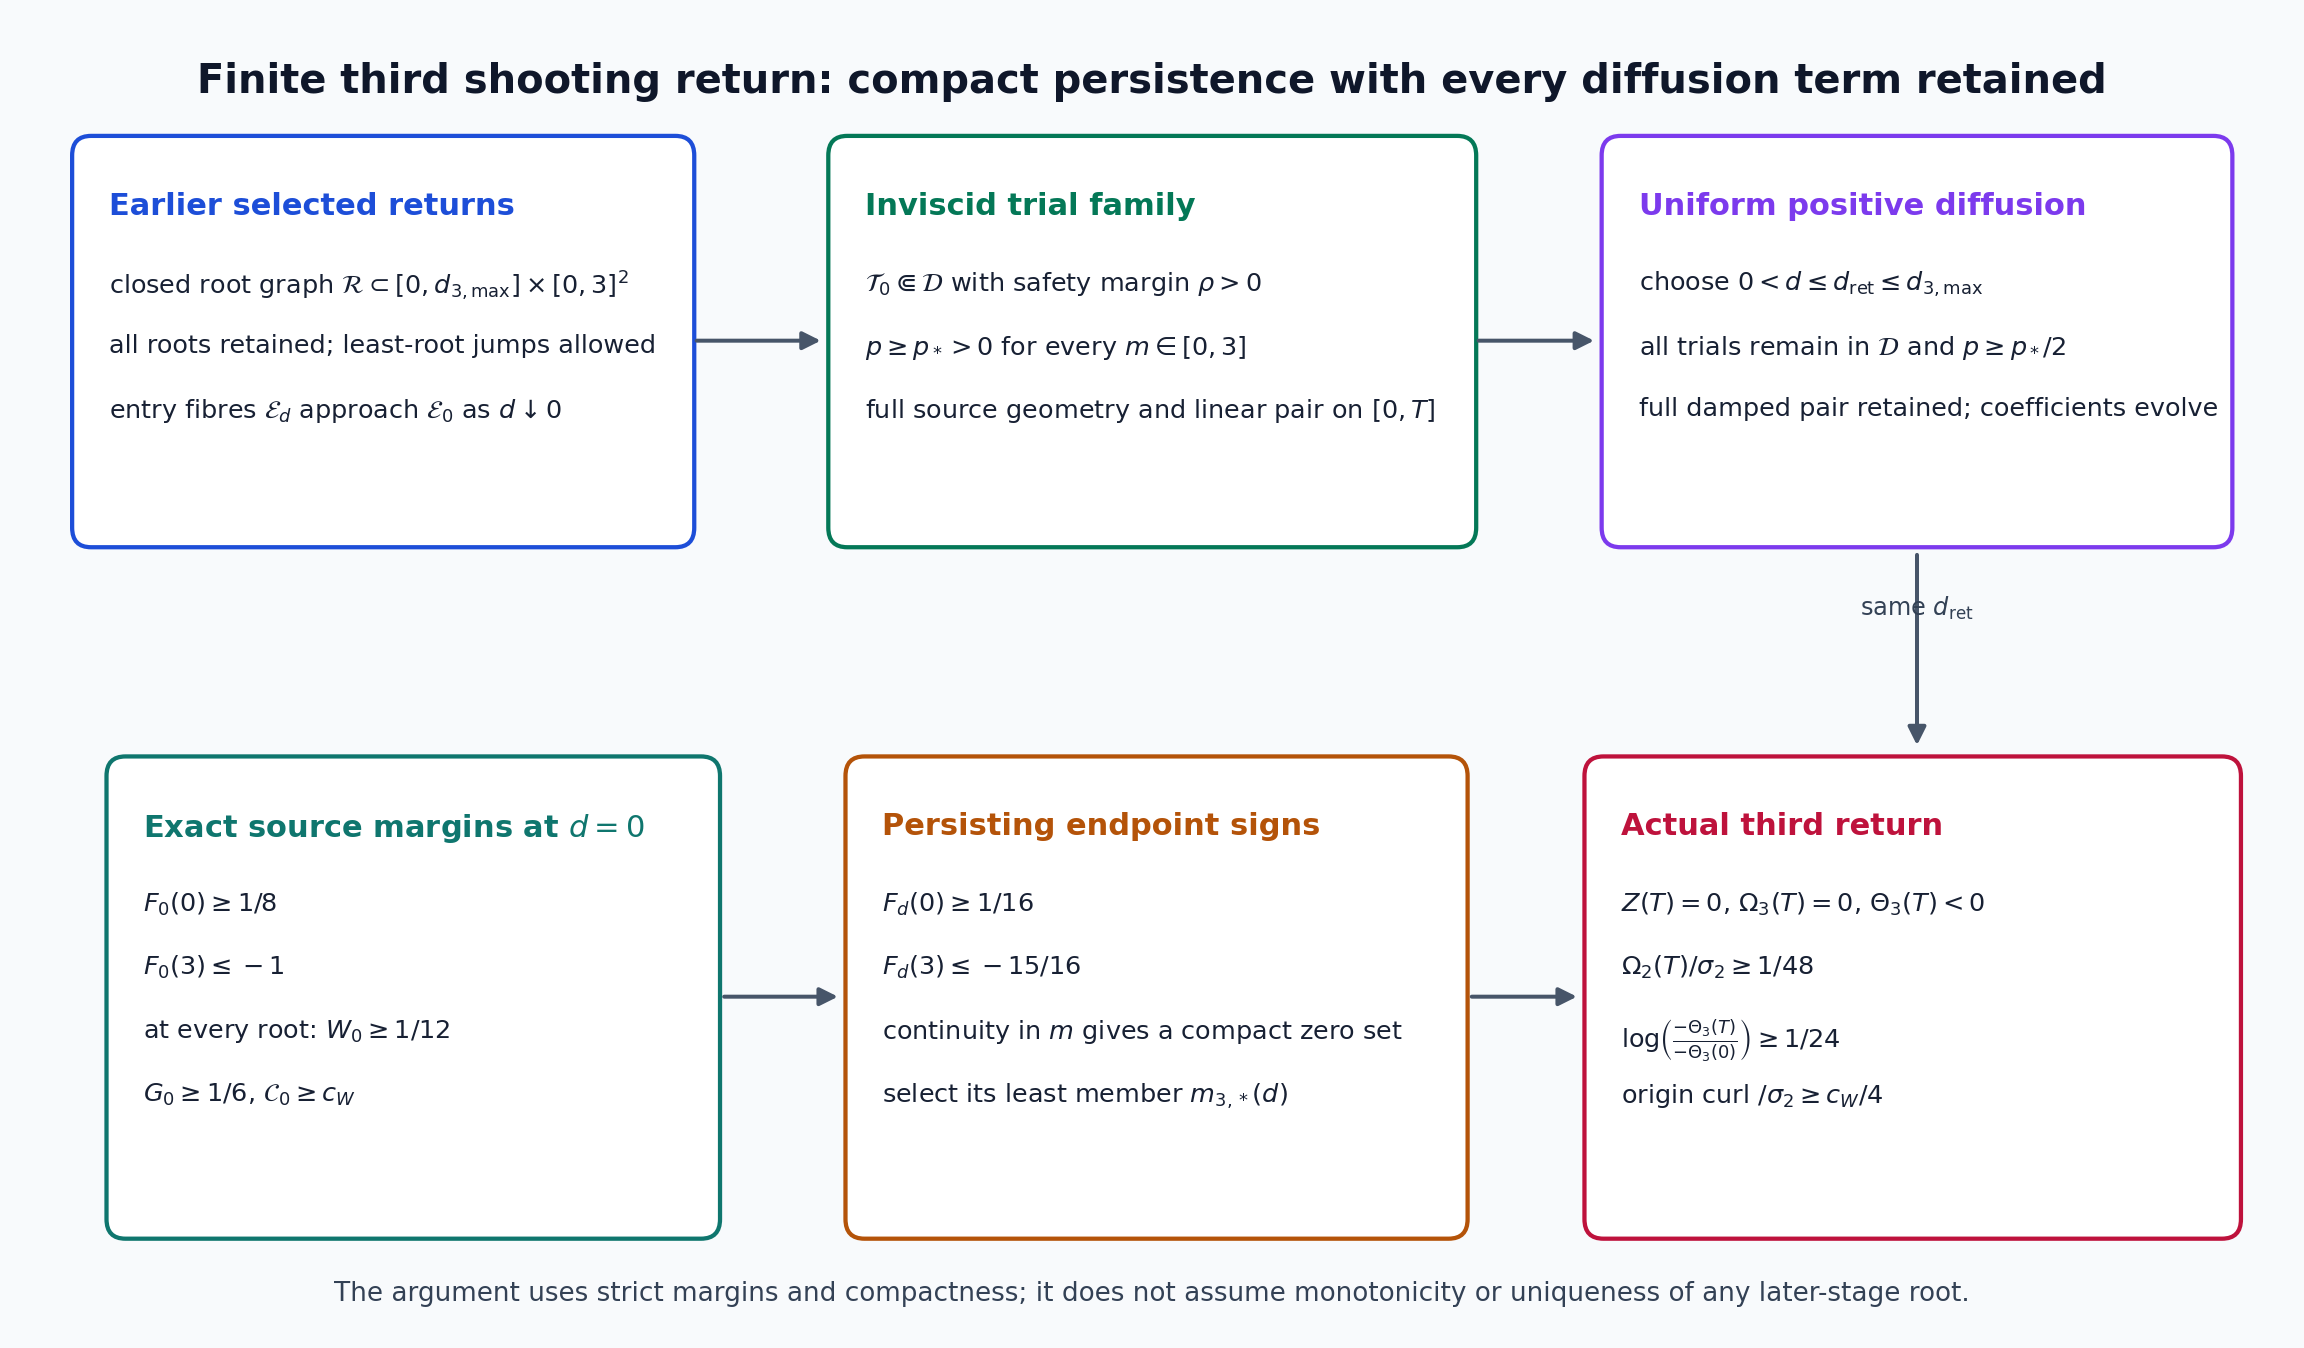
\includegraphics[width=0.96\linewidth]{third_return/figures/third_return_persistence.png}
 \caption{The exact finite persistence argument.  The inviscid entry and
 trial set has a compact trajectory image strictly inside the smooth
 component domain.  The closed earlier-root graph and uniform ODE
 continuation keep the positive-diffusion family in that interior.  The
 source endpoint margins persist, forcing a third endpoint zero and the
 displayed return bounds.  No monotonicity of the shooting map is used.}
 \label{trc:fig:persistence}
\end{figure}

\section{Compact spatial realization of the actual local third steering}
\label{trls:section}

The interval in Theorem~\ref{tr:local} has a complete compact
realization with the original periodic profile and physical diffusion.
We prove the substituted material, support, amplitude, and force
bounds here. Both older vorticities remain variables in this
realization. We also construct an explicit right continuation of the
same steering, which supplies a smooth compact time extension of its
forces. The required endpoint in this section is the local steering
endpoint, without an assertion about the full negative pulse.

\subsection{A proved interval, amplitude bounds, and material matrices}

Retain all the data of Theorem~\ref{tr:local}, and put
\begin{equation}\label{trls:times}
 \begin{gathered}
 \tau=\Gamma(t-t_1),\quad \tau_0=\sin s/8192,\quad
 t_*=t_1+\frac1{8192\sigma_2},\\
 \epsilon_R=\frac1{16384\sigma_2},\qquad
 I_*=[t_1,t_*],\quad I_+=[t_1,t_*+\epsilon_R].
 \end{gathered}
\end{equation}
Thus $0\leq\tau\leq3\tau_0/2$ on $I_+$, and the
original source steering remains its first ramp
$Z=Z_1(1-\eta(\tau))$ throughout. In particular every original
trial $m\in[0,3]$ gives the same solution on this interval.

The existence argument in Theorem~\ref{tr:local} extends to
this entire $I_+$. Indeed on the same closed cube of radius
$1/128$ about its actual six-dimensional entry state, the norm of
the scaled vector field is strictly less than $32/\sin s$.
On $0\leq\tau\leq3\tau_0/2$ its integral can therefore
move the state by at most
\[
 \frac{32}{\sin s}\frac{3\sin s}{2\cdot8192}
     =\frac3{512}<\frac1{128}.
\]
A first exit from that cube is impossible. Its fixed positive
denominator margins and bounded smooth derivatives extend the
unique solution to this closed interval, by the same integral-equation
argument. This proves a continuation of the actual source control,
including all its endpoint derivatives.

Write the dimensionless state as in \eqref{tr:scaled}, with
$E=E_1/\sigma_1^2$, $F_2^{\rm amp}=E_2/\sigma_2^2$,
$\omega=\Omega_1/\sigma_1$ and $V=\Omega_2/\sigma_2$.
To avoid confusing the second amplitude with the original periodic
profile $F$, denote $F_2^{\rm amp}$ by $F_a$ below. On all of
$I_+$ the already verified cube gives
\begin{equation}\label{trls:cube}
 \begin{gathered}
 63/64<h<4,\quad 11/16<g<6,\quad
 15/128<E<3,\quad 7/128<F_a<4,\\
 |\omega|<11,\quad |V|<1/16,\quad
 15/16<D=h^2+a^2<17,\\
 0\leq Z\leq Z_1<(9/8)\sin s<1/128,\\
 b=r_b\sin s<4\sin s,\quad 1\leq r_b\leq\sqrt{10}.
 \end{gathered}
\end{equation}
Use the exact $x,y,R,Y$ and phases in
\eqref{tr:coordinates}--\eqref{tr:inverse}. Then
\begin{equation}\label{trls:phasebounds}
 \frac1{64}<R=\frac{g^2+b^2}{D}<39,
 \qquad Y>1/9,\qquad 0<x<7,\quad 0<y<7.
\end{equation}
For the upper bound on $R$, use
$(36+16/512^2)/(15/16)<39$. Its lower bound and that of
$Y$ are the inequalities proved on the same cube in
Theorem~\ref{tr:local}. Positivity of $x,y$ is also proved
there; $x^2+y^2=R<39<49$ gives their upper bounds.
All three second components stay positive by the exact inverse,
without imposing a sign on either older vorticity.

We prove an explicit bound for the newest amplitudes. Set
\[
 X=-\Theta_3/P_3^*,\qquad
 W=-\sigma_2\Omega_3/(K_3P_3^*),\qquad
 \mathcal K=\frac{N_3}{\sigma_2^2\sin s\,R},\qquad
 \mathcal B=\frac Z{\sin s}.
\]
The exact pair \eqref{tr:physical_pair} becomes
\begin{equation}\label{trls:pair}
 X'=\mathcal K W-\delta_3RX,\qquad
 W'=\mathcal B X-\delta_3RW,
 \qquad \delta_3=dK_3^2/\Gamma.
\end{equation}
Its entry values satisfy $0<X(0)\leq e^4$ and
$0<W(0)\leq3e^4$ by the actual transition theorem.
The older geometry is already constructed on the compact interval
$I_+$, so the coefficient matrix of \eqref{trls:pair} is smooth
and bounded there. Its iterated integral series converges uniformly:
if its matrix norm is bounded by $B$, the term with $n$ integrals
is bounded by $(B\tau)^n/n!$ times the initial norm.
The series solves the integral equation, and the same iterated
estimate on the difference of two solutions proves uniqueness.
It therefore constructs the newest pair through all of $I_+$
independently of the following sign argument.
On the cube $N_3>0$, since $E_1,E_2,c,C,x,y,b$ are positive.
Removing the common damping and integrating the resulting positive
off-diagonal linear system proves $X,W>0$ throughout $I_+$.
More explicitly, a first zero of either positive coordinate would
contradict its positive initial value plus the integral of a
nonnegative multiple of the other coordinate.

There is a useful bound on $\mathcal K$ that retains the source
scale ratio. With $q=\sigma_1/\sigma_2=s/L$,
$\bar c=c/\sigma_1^2\leq1/4$ and
$\bar C=C/\sigma_1^2\leq a/32$, the exact numerator is
\[
 \frac{N_3}{\sigma_2^2\sin s}
 =\frac{q^2}{\sin s}\{(E+\bar c)y+\bar Cx\}
       +r_bF_a.
\]
The expression in braces is less than
$7(13/4+1/16384)<25$. Furthermore
\[
 \frac{q^2}{\sin s}=\frac{s^2}{L^2\sin s}
 \leq\frac{16s}{15L^2}
 \leq\frac{16}{15\cdot512\cdot16384^2},
 \qquad
 \frac{25\cdot16}{15\cdot512\cdot16384^2}<1.
\]
Here $\sin s\geq15s/16$ is the established source angle
estimate. Thus $0<N_3/(\sigma_2^2\sin s)<17$ and
\begin{equation}\label{trls:pairbox}
 0<\mathcal K<1088,\qquad 0\leq\mathcal B<9/8.
\end{equation}
Since $X,W>0$, addition of \eqref{trls:pair} gives
$(X+W)'\leq1089(X+W)$. Multiplication by
$e^{-1089\tau}$ and integration show
\[
 X+W\leq4e^4e^{1089\tau},\qquad
 1089\tau\leq\frac{3267\sin s}{16384}<\frac14.
\]
The power series gives $e^z\leq\sum_{n\geq0}z^n
=(1-z)^{-1}\leq4/3$ for $0\leq z\leq1/4$.
Consequently on the required interval and its proved right collar,
\begin{equation}\label{trls:amplitudes}
 0<-\Theta_3<6e^4P_3^*,\qquad
 |\Omega_3|<6e^4K_3P_3^*/\sigma_2.
\end{equation}
This uses the signed linear pair before any quotient estimate.

The exact matrices remain \eqref{tr:matrices}; all retain their
original birth times. With $h_0=\cos s_2$ and
$N=1+(3-h_0)/a$, define
\begin{equation}\label{trls:matrixbounds}
 \mathsf N_1=1,\qquad \mathsf N_2=2N,\qquad
 \mathsf N_3=32/\sin s.
 \qquad
 \|M_j\|,\|M_j^{-1}\|\leq\mathsf N_j.
\end{equation}
For the second matrix, the triangular factor and its inverse have
norm at most $1+|h-h_0|/a$. Since $h>0$, $h<4$, and
$h_0<1$, one has $|h-h_0|<4-h_0$. The difference
$2N-[1+(4-h_0)/a]=1+(2-h_0)/a$ is positive.
For the third, use $\mathcal L=(\zeta_2\ \zeta_3)$.
Its determinant is $-b$ and
$\|\mathcal L\|_F^2=D+R<56$, whereas
$\|\mathcal L(t_b)\|_F^2=r_b^2+1\leq11$.
The adjugate identity for two by two matrices therefore bounds
both products defining $M_3$ and its inverse by
$\sqrt{616}/b<32/\sin s$. This calculation allows both
older shears to evolve. The matrices have determinant one and
define the same global linear diffeomorphisms of $\mathbb R^2$.

\subsection{Support nesting with the unchanged source choice}

Let $C_M,C_N$ and $Y_3$ retain their exact values in
\eqref{tge:Y3} and \eqref{tts:sourceconstants}. Put
\[
 p=47Q_2/16-3,\qquad r=(31Q_2+1)/16.
\]
The literal outer $+1$ in \eqref{tge:Y3} gives the strict
stronger margins
\begin{equation}\label{trls:sourcemargins}
 \widehat\lambda_1^p\geq e^p(4C_NC_M),\qquad
 \widehat\lambda_1^r\geq e^r\sqrt{11}C_M/s_0.
\end{equation}
Indeed $\log\widehat\lambda_1\geq Y_3$ is at least one
plus either logarithmic summand divided by its positive exponent.
Also $N\leq C_N\widehat\lambda_1^{1/16}$ and
$\mathsf N_3\leq2C_M
\widehat\lambda_1^{(Q_2-1)/16}$, by
\eqref{tts:sourceconstants}. Multiplying these exact powers
proves
\begin{align*}
 \frac{2\mathsf N_2\mathsf N_3
                  \widehat\lambda_2^{-3}}
      {\widehat\lambda_1^{-3}}&\leq2e^{-p}<1,\\
 \frac{\sqrt{17}\mathsf N_3
                  \widehat\lambda_2^{-2}}{s_0}
     &\leq2\sqrt{17/11}\,e^{-r}<1.
\end{align*}
For the last strict inequalities, $Q_2\geq202$ implies
$p>1$ and $r>2$. The elementary inequality $e^z\geq1+z$
therefore gives $e^p>2$ and $e^r>3$, and
$2\sqrt{17/11}<3$ follows from $68<99$.
The earlier source margins give
\begin{equation}\label{trls:nestingnumbers}
 \begin{gathered}
 2\mathsf N_2\mathsf N_3\widehat\lambda_2^{-3}
      <\widehat\lambda_1^{-3},\quad
 \sqrt{17}\mathsf N_3\widehat\lambda_2^{-2}<s_0,\\
 \mathsf N_2\widehat\lambda_1^{-3}<s_0/(2C_\ell),
 \qquad \mathsf N_2\widehat\lambda_1^{-2}<s_0.
 \end{gathered}
\end{equation}
For the last two use $\mathsf N_2=2N$ and the proved
first-source margins $N\widehat\lambda_1^{-3}
<s_0/(4C_\ell)$ and $N\widehat\lambda_1^{-2}<s_0/2$.

Keep exactly the radii, periodic $F$, its even zero-mean primitive
$P$, and material cutoffs in \eqref{tts:envelopes}.
For every $t\in I_+$ a third support point satisfies
$|x|\leq\mathsf N_3\ell_3$. Thus
\[
 |M_2^{-1}x|\leq\mathsf N_2\mathsf N_3\ell_3<\ell_2/2,
 \qquad |K_2\zeta_2\cdot x|
    <K_2\sqrt{17}\mathsf N_3\ell_3<s_0.
\]
The entire second field is affine in a neighborhood of that point.
For every second support point the last two inequalities in
\eqref{trls:nestingnumbers} give $|x|<\ell_1/2$ and
$|K_1\zeta_1\cdot x|<s_0$. The first material matrix is
a rotation, so the first envelope is one there and its profile
is linear. Finally the original first support remains inside the
original affine cell of the radial base. The same inclusions hold
for every derivative support because their containing closed supports
are unchanged. All the inequalities are strict, so these are open
affine neighborhoods in the original physical coordinates.

\subsection{Full fields and exact scalar and vector equations}

Define the base and all three increments by
\eqref{tts:base} and \eqref{tts:fields}, using the exact
solution on $I_+$. All activation weights are one on this interval.
The fields agree at $t_1$, with every derivative, with the already
constructed fields through the third transition: the exact control
and phase jets match by the proof of Theorem~\ref{tr:local},
and repeated differentiation of the amplitude and material equations
matches their jets. They therefore give one smooth field on
$[0,t_*+\epsilon_R]$, with the original sine initial temperature
and zero initial velocity.

Use the exact scalar and full vector increments
\eqref{tts:Qrest}--\eqref{tts:spatialjets}, and the base
and total forces \eqref{tts:baseforce}. These formulas remain
the full residuals on $I_+$, as can be checked directly here.
On a $j$th support the proved older field is precisely
$G_{<j}\cdot x$ and $D_{<j}x$ with the unchanged sums in
\eqref{tts:material}. The identities
$\partial_t k_j=-D_{<j}^Tk_j$ and
$\partial_t M_j^{-1}=-M_j^{-1}D_{<j}$ give
\[
 (\partial_t+D_{<j}x\cdot\nabla)\xi_j=0,
 \qquad
 (\partial_t+D_{<j}x\cdot\nabla)g_j=0.
\]
In the scalar equation, the $F g_j$ part of
$v_j\cdot G_{<j}$ cancels the exact $\dot\Theta_j$
coupling, leaving the cutoff term, self-advection, modal damping,
and full Laplacian exactly as in \eqref{tts:scalarforce}.
In the vector equation, trace zero gives
$D_{<j}J+JD_{<j}^T=0$, whence the material derivative of
$J\nabla\Psi_j$ contributes $D_{<j}v_j$.
The reverse interaction $(v_j\cdot\nabla)(D_{<j}x)$
is a second $D_{<j}v_j$. Adding its other terms gives
\eqref{tts:vectorforce}, including both parent velocities,
the full buoyancy, and the moving-length term in $Q_{\rm r}$.
Adding the three identities counts every ordered older/newer
interaction once; outside their supports every derivative vanishes.
The identities therefore hold globally on $\mathbb R^2$.

Together with the base residual this proves exactly
\eqref{tts:PDE} on $[0,t_*+\epsilon_R]$, with $p=0$.
The streamfunction identity gives $\operatorname{div}u=0$.
Every spatial support remains in $B_{R_H}$ by the proved nesting.
The phase-coordinate Laplacian is still precisely
\eqref{tts:metric}, with its evolving positive matrix
$M_j^{-1}M_j^{-T}$ and all mixed derivatives. On a linear
profile cell the viscous force still includes
$-d\rho_jV_j$ and $-d\rho_jv_j$; the corresponding
Laplacians vanish there by \eqref{tts:core}. The full fields
retain the constant $P(0)$ in their cutoff region. Thus the
original profile has not been replaced by a modal eigenfunction.

\subsection{Actual all-order spatial and diffusion costs}

The following explicit data hold on the whole proved $I_+$:
\begin{equation}\label{trls:normdata}
 \begin{gathered}
 \mathsf r_{-,j}^2=(1,15/16,1/64)_j,\qquad
 \mathsf r_{+,j}^2=(1,17,39)_j,\quad
 \mathsf\kappa_j=K_j\mathsf r_{+,j},\\
 \mathsf U_{\Theta,j}=
 (3\sigma_1^2/K_1,\ 4\sigma_2^2/K_2,\ 6e^4P_3^*)_j,\\
 \mathsf U_{\Omega,j}=
 (11\sigma_1,\ \sigma_2/16,\ 6e^4K_3P_3^*/\sigma_2)_j,
 \qquad W_{j,1}=0,\\
 \mathsf A_*=693\sigma_1+12\Gamma
           +(81/8)\Gamma\sin s\,[\eta']_0.
 \end{gathered}
\end{equation}
The older data are the actual cube estimates, rather than their
smaller preceding-transition bounds. To verify
$|\dot\alpha|\leq\mathsf A_*$, use \eqref{tr:control}.
Here $Y>1/9$, $y<7$, $|\zeta_{1,1}|\leq1$,
$|\zeta_{2,1}|<5$, $b/D<(64/15)\sin s$,
$|\Omega_1|<11\sigma_1$, and
$|\Omega_2|<\sigma_2/16$. Therefore
\[
 |\mathcal F_3|
 <9\left(77\sigma_1+
   \frac{64\sin s}{15}\frac{\sigma_2}{16}\,5\right)
 =693\sigma_1+12\Gamma.
\]
The other control term has size
$|\dot Z|/Y\leq(81/8)\Gamma\sin s[\eta']_0$,
which proves the stated bound using the exact source derivative.

The following finite sums specify every spatial cost, with
$f_m,[F]_m,[P]_m,H_m,c_m$ defined as in Section~\ref{tts:section}:
\begin{align}\label{trls:costdefinitions}
 \mathsf D_j&=\mathsf A_*+\sum_{i<j}\mathsf U_{\Omega,i},&
 \mathsf G_j&=A_0+\sum_{i<j}K_i\mathsf U_{\Theta,i}
                                      \mathsf r_{+,i},\nonumber\\
 \mathsf Q_j&=\frac{\mathsf U_{\Omega,j}}
                         {K_j^2\mathsf r_{-,j}^2},&
 \mathsf Q_{{\rm r},j}&=
 \frac{\mathsf\kappa_j\mathsf U_{\Theta,j}
                   +2\mathsf D_j\mathsf U_{\Omega,j}}
      {K_j^2\mathsf r_{-,j}^2},\\
 \mathsf e_{j,m}&=(\mathsf N_j/\ell_j)^mf_m,&
 \mathsf B_{j,m}(W)&=\sum_{q=0}^m\binom mq
          \mathsf\kappa_j^q[W]_q\mathsf e_{j,m-q},\nonumber\\
 \mathsf C_{j,m}(P)&=\sum_{q=0}^m\binom mq
          \mathsf\kappa_j^q[P]_q\mathsf e_{j,m-q+1}.&&\nonumber
\end{align}
In the occurrences $\mathsf B_{j,m}(W)$ the argument is a
periodic test profile, not the signed amplitude $W$ of
\eqref{trls:pair}. The operator norm of
$J\zeta_i\otimes\zeta_i/r_i^2$ equals one, so
$\|D_{<j}\|\leq\mathsf D_j$ with the entire second
vorticity included. The gradient sum similarly gives
$|G_{<j}|\leq\mathsf G_j$. Differentiating
$\rho_j$ gives $|\dot\rho_j/\rho_j|\leq2\mathsf D_j$.
These prove the bounds $|Q_j|\leq\mathsf Q_j$ and
$|Q_{{\rm r},j}|\leq\mathsf Q_{{\rm r},j}$.
The product rule with its $\binom mq$ allocations and the
linear material bound \eqref{trls:matrixbounds} proves
$|W(\xi_j)g_j|_m\leq\mathsf B_{j,m}(W)$ and
$|P(\xi_j)\nabla g_j|_m\leq\mathsf C_{j,m}(P)$.

In particular the complete damping and diffusion terms obey
\begin{align}\label{trls:diffusioncost}
 \mathsf D_{\theta,j,m}
 &=d\mathsf U_{\Theta,j}
   \{\mathsf\kappa_j^2\mathsf B_{j,m}(F)
                     +2\mathsf B_{j,m+2}(F)\},\nonumber\\
 \mathsf D_{u,j,m}
 &=d\mathsf Q_j
   \{\mathsf\kappa_j^2\mathsf B_{j,m+1}(P)
                     +2\mathsf B_{j,m+3}(P)\}.
\end{align}
The two coordinate traces of the Laplacian account for the factor
two in each expression. Direct termwise application to the full
residuals proves the bounds
\begin{align}\label{trls:forcecost}
 \mathsf E_{\theta,j,m}={}&
 \mathsf Q_j\mathsf G_j\mathsf C_{j,m}(P)
                     +\mathsf D_{\theta,j,m}\nonumber\\
 &+\mathsf Q_j\mathsf U_{\Theta,j}
    \sum_{q=0}^m\binom mq
       \mathsf B_{j,q+1}(P)\mathsf B_{j,m-q+1}(F),\nonumber\\
 \mathsf E_{u,j,m}={}&
 (2\mathsf D_j\mathsf Q_j+\mathsf Q_{{\rm r},j})
                  \mathsf B_{j,m+1}(P)
 +\mathsf U_{\Theta,j}\mathsf B_{j,m}(F)
 +\mathsf D_{u,j,m}\nonumber\\
 &+\mathsf Q_j^2\sum_{q=0}^m\binom mq
       \mathsf B_{j,q+1}(P)\mathsf B_{j,m-q+2}(P),\\
 |E_{\theta,j}|_m\leq{}&\mathsf E_{\theta,j,m},\qquad
 |E_{u,j}|_m\leq\mathsf E_{u,j,m}.\nonumber
\end{align}
Indeed the scalar product sum bounds
$v_j\cdot\nabla V_j$; the vector sum bounds
$(\nabla v_j)v_j$, allocating all $m$ derivatives in
each case. The remaining terms are exactly the linear terms of
\eqref{tts:scalarforce} and \eqref{tts:vectorforce}.
There is no activation derivative on $I_+$ because all weights
are one.

Let $B_{0,m}(F)=\sum_{q=0}^m\binom mq\mu^q[F]_qc_{m-q}$.
The control constant $\mathsf A_2$ bounding $|\ddot\alpha|$
is explicitly defined below. The base and sums now give global norms
on the original $\mathbb R^2$:
\begin{align}\label{trls:globalnorms}
 |\theta|_m&\leq(A_0/\mu)B_{0,m}(F)
       +\sum_{j=1}^3\mathsf U_{\Theta,j}\mathsf B_{j,m}(F),
 \nonumber\\
 |u|_m&\leq\mathsf A_*H_m
       +\sum_{j=1}^3\mathsf Q_j\mathsf B_{j,m+1}(P),\nonumber\\
 |f_\theta|_m&\leq2d(A_0/\mu)B_{0,m+2}(F)
                       +\sum_{j=1}^3\mathsf E_{\theta,j,m},\\
 |f_u|_m&\leq\mathsf A_2H_m
       +\mathsf A_*^2\sum_{q=0}^m\binom mqH_{q+1}H_{m-q}
       +(A_0/\mu)B_{0,m}(F)+2d\mathsf A_*H_{m+2}
                       +\sum_{j=1}^3\mathsf E_{u,j,m}.\nonumber
\end{align}
These follow from the displayed fields and base residual; the
initial interpolation is already complete on $I_+$. They bound
the entire fields and forces, not only their common affine cell.
For each fixed bound in this display, integration over the required
interval multiplies it by $1/(8192\sigma_2)$; over $I_+$ the
factor is $3/(16384\sigma_2)$. The earlier proved norms together
with these, taking the maximum on their two adjacent intervals,
give the corresponding bounds through $t_*$.

The exact retained localization and newest diffusion factors include
\begin{equation}\label{trls:frequencycost}
 \begin{gathered}
 \mathsf N_1/\ell_1=C_\ell\mu/s_0,\quad
 \mathsf N_2/\ell_2=2N\mu\widehat\lambda_1^3,\quad
 \mathsf N_3/\ell_3=
                32\mu\widehat\lambda_2^3/\sin s,\\
 d\mathsf U_{\Theta,3}K_3^2
       =6e^4dA_0\mu\widehat\lambda_3^{9/8},\quad
 d\mathsf Q_3K_3^3
       =384e^4dA_0\mu\widehat\lambda_3^{9/8}/\sigma_2.
 \end{gathered}
\end{equation}
They are explicit factors in upper force costs. The exact three
modal exponents over $I_*$ are
\begin{equation}\label{trls:exponents}
 dK_1^2|I_*|,\qquad dK_2^2\int_{I_*}D\,dt,\qquad
 dK_3^2\int_{I_*}R\,dt.
\end{equation}
The second is between $(15/16)dK_2^2|I_*|$ and
$17dK_2^2|I_*|$, and the third between
$dK_3^2|I_*|/64$ and $39dK_3^2|I_*|$.
The exact newest gain is \eqref{tr:costs} with
$\tau_f=\tau_0$; all divisions there are valid by positivity
of the pair just proved. Both older numerator-loss terms in
\eqref{tr:losses} remain present, separately from these modal
exponents.

\subsection{Exact source jets, mixed costs, and compact time forces}

We give an explicit finite recursion for all control derivatives.
Let $z=(h,g,E,F_a,\omega,V,X,W)$ and introduce the switch jets
$\lambda^{[j]}$. Define $Z=Z_1(1-\lambda^{[0]})$,
and use the exact inverse \eqref{tr:inverse} with this $Z$.
The eight-dimensional vector field $\mathcal V^{\rm loc}$
uses the coordinate right-hand sides in \eqref{tr:scaled}
with $F=F_a$, ordered as $(h,g,E,F_a,\omega,V)$,
followed by the two right-hand sides in \eqref{trls:pair}.
In particular it depends
on $\lambda^{[0]}$, not its derivatives. Define the exact
physical angular function
\begin{equation}\label{trls:controlfunction}
 \Phi(z,\lambda^{[0]},\lambda^{[1]})
  =\frac{\sigma_1\omega y\zeta_{1,1}
           +(b\sigma_2V/D)\zeta_{2,1}
           +\Gamma Z_1\lambda^{[1]}}{Y}.
\end{equation}
Substituting $\lambda^{[j]}=\eta^{(j)}(\tau)$ gives
exactly $\dot\alpha$ in \eqref{tr:control}, because
$\dot Z=-\Gamma Z_1\eta'(\tau)$.
Thus every source-ramp derivative retains its original factor
$\Gamma^rZ_1$. No constant switch is used on the collar.

On the explicit compact rectangle
\begin{equation}\label{trls:jetbox}
 \begin{gathered}
 h\in[63/64,4],\quad g\in[11/16,6],\quad
 E\in[15/128,3],\quad F_a\in[7/128,4],\\
 \omega\in[-11,11],\quad V\in[-1/16,1/16],\quad
 X,W\in[0,6e^4],\quad \lambda^{[0]}\in[0,1],
 \end{gathered}
\end{equation}
the estimates for $D,R,Y$ used above are uniform and positive.
The same elementary inequalities apply at its boundary, since their
final margins are strict even with all displayed weak bounds.
The vector field and $\Phi$ are consequently smooth on a
neighborhood of this rectangle for any finite control-jet bounds.
Define the derivation
\begin{equation}\label{trls:jetderivation}
 \mathcal C_{\rm loc}
 =\sum_{l=1}^8\mathcal V_l^{\rm loc}
                   \partial_{z_l}
   +\sum_{j\geq0}\lambda^{[j+1]}
                   \partial_{\lambda^{[j]}}.
\end{equation}
Each application to a finite expression uses only finitely many
terms. The chain rule gives, by induction on $n$,
\begin{equation}\label{trls:controljets}
 \begin{gathered}
 \alpha^{(n+1)}=
       \Gamma^n\mathcal C_{\rm loc}^n\Phi
       \big|_{\lambda^{[j]}=\eta^{(j)}(\tau)},\\
 \mathsf A_{n+1}=\Gamma^n\max
 \left\{|\mathcal C_{\rm loc}^n\Phi|:
    z,\lambda^{[0]}\text{ in \eqref{trls:jetbox}},
    \ |\lambda^{[j]}|\leq[\eta^{(j)}]_0,
                            \ 1\leq j\leq n+1\right\},\quad n\geq0.
 \end{gathered}
\end{equation}
These are finite maxima of specified elementary expressions on
specified compact rectangles. They contain no supremum over a
future trajectory. The preceding identity proves
$|\alpha^{(n+1)}|\leq\mathsf A_{n+1}$; the sharper
$\mathsf A_*$ in \eqref{trls:normdata} may be used at first
order. In particular the base constant in
\eqref{trls:globalnorms} is precisely $\mathsf A_2$.

For clarity, the induction behind the displayed identity differentiates
a function of $z$ along its eight exact state rows and differentiates
each $\eta^{(j)}$ to $\eta^{(j+1)}$. Physical time
adds a factor $\Gamma$ at each step. Conversely substituting
the state scalings into these rows recovers the six older physical
equations and newest physical pair; their inverse scalings are
exact and all scale denominators are positive.

All mixed space and time norms are then evaluated by the complete
pullback operators \eqref{tts:pullbackops} and their identity
\eqref{tts:pullbackidentity}, replacing the transition derivation
by \eqref{trls:jetderivation} and its rectangle by
\eqref{trls:jetbox}. Explicitly start from the zeroth constants
\eqref{trls:matrixbounds} and \eqref{trls:normdata} and
differentiate
\[
 \dot M_j=D_{<j}M_j,\qquad
 \dot A_j=-A_jD_{<j},\qquad
 \dot k_j=-D_{<j}^Tk_j,\qquad A_j=M_j^{-1}/\ell_j.
\]
For example
$\partial_t^{n+1}A_j=-\sum_{q=0}^n\binom nq
(\partial_t^qA_j)(\partial_t^{n-q}D_{<j})$.
The product rule gives the other two recursions with the displayed
matrix order and signs. Coefficient jets of the parent sums are
given by \eqref{trls:jetderivation}; all activation jets on
$I_+$ vanish. On every layer support bound each factor $x^\beta$
in the pullback expression by
$(\mathsf N_j\ell_j)^{|\beta|}$, each periodic derivative
by its original $[F]_r$ or $[P]_r$, and each envelope derivative
by $f_r$. Sum the resulting finite absolute products with the
binomial coefficients produced by these recursions. The chain and
product rules prove the resulting bound for every prescribed mixed
order. On the base use $R_H$, its fixed profile derivatives, and
\eqref{trls:controljets} instead. The recursion has finite depth
equal to the requested derivative order and retains every time
derivative of the actual Laplacian metric and modal diffusion.

Finally extend the original sine datum constantly to negative time
with zero velocity as in Section~\ref{tts:section}, and take
$\epsilon_L=1/\nu$. Let $f_\bullet^{\rm raw}$ be the full
residuals \eqref{tts:rawcollar} of these fields on
$[-\epsilon_L,t_*+\epsilon_R]$. On the nonnegative interval
they equal the proved telescoping force formulas. Define
\begin{equation}\label{trls:timecutoff}
 \beta_*(t)=\eta(1+t/\epsilon_L)
             \eta(1+(t_*-t)/\epsilon_R),\qquad
 \widetilde f_\bullet=\beta_*f_\bullet^{\rm raw}.
\end{equation}
Here the right collar is the actual source steering continuation
already constructed, with physical length $\epsilon_R$ in
\eqref{trls:times}. The cutoff equals one on $[0,t_*]$;
flatness of the original step makes extension by zero smooth at
both outer times. The forces are therefore smooth and compact in
space and time, and solve the exact PDE on the entire required
$[0,t_*]$. Their complete cutoff costs are
\begin{equation}\label{trls:cutoffcost}
 \begin{gathered}
 \mathsf B_{\beta,r}=\sum_{q=0}^r\binom rq
      \epsilon_L^{-q}\epsilon_R^{-(r-q)}
       [\eta^{(q)}]_0[\eta^{(r-q)}]_0,\\
 \|\partial_t^n\partial_x^\gamma\widetilde f_\bullet\|_\infty
 \leq\sum_{q=0}^n\binom nq\mathsf B_{\beta,q}
  \|\partial_t^{n-q}\partial_x^\gamma
                                f_\bullet^{\rm raw}\|_\infty.
 \end{gathered}
\end{equation}
The raw mixed norms on $I_+$ have the explicit recursion just
proved, those on the preceding slab have the proved earlier
recursions, and those on the constant left extension are obtained
by differentiating its fixed sine datum and residual. Taking their
maximum gives every norm in \eqref{trls:cutoffcost}.

Oddness of the original scalar profile, evenness of its primitive
and cutoffs, and the linear material maps give the same odd
temperature, velocity and forces and even vorticity as before.
The compact smooth streamfunction has finite-energy velocity and
still satisfies the exact Biot--Savart identity proved in
Section~\ref{tts:section}. Thus the local source steering, its
moving endpoint, and its proved right collar have a complete
compact original-profile PDE realization with all physical
diffusion, localization, and control costs specified.

\section{Exact coupled feedback and the scope of common damping}
\label{sec:feedback}
Retain the source layer frequencies $\lambda_j$, and write
$K_j=\mu\lambda_j$ for physical frequencies. Let $\Theta_j,
\Omega_j$ denote physical amplitudes. For each activated layer
$j$, let $\zeta_j\ne0$, $r_j=|\zeta_j|$, $e_j=\zeta_j/r_j$,
$S_j=Je_j\otimes e_j$, and $A_j=-K_jr_j\Theta_j$.
The exact physical counterpart of source (3.3)--(3.5) is
\begin{align}
 G_{<q}&=-A_0e_0+\sum_{j<q}w_jK_j\Theta_j\zeta_j,
 &D_{<q}&=\dot\alpha J+\sum_{j<q}w_j\Omega_jS_j,\notag\\
 \dot M_q&=D_{<q}M_q,\quad M_q(t_q^{\rm in})=I,
 &\zeta_q&=M_q^{-T}p_q,\notag\\
 \dot\zeta_q&=-D_{<q}^T\zeta_q,
 &\dot\Theta_q&=-\frac{J\zeta_q\cdot G_{<q}}{K_qr_q^2}\Omega_q,
 \quad\dot\Omega_q=K_q\zeta_{q,1}\Theta_q.
 \label{eq:physicalcoupled}
\end{align}
Each sum begins at $j=1$, and contains finitely many terms at
every finite preterminal time. The rotating base coefficient
is the original $A_0$, not a reset unit value. The physical
growth-scale definition is $\sigma_q^2=|G_{<q+1}(t_q^b)|$,
so $\sigma_q=\nu\widetilde\sigma_q$.

For $\zeta_{j,2}\ne0$ define
\begin{equation}
 \mathcal F_j=-\frac{\sum_{i<j}w_i\Omega_i e_{i,1}
 (Je_i\cdot\zeta_j)}{\zeta_{j,2}},\qquad \mathcal F_0=0.
 \label{eq:physicalfeedback}
\end{equation}
Transposing $S_i$ gives
$S_i^T\zeta_j=e_i(Je_i\cdot\zeta_j)$, and the first
component of $-\dot\alpha J^T\zeta_j$ is
$-\dot\alpha\zeta_{j,2}$. Hence
\begin{equation}
 \dot\zeta_{j,1}=(\mathcal F_j-\dot\alpha)\zeta_{j,2}.
 \label{eq:controlledcomponent}
\end{equation}
It follows by direct differentiation that
$\dot\alpha=\mathcal F_j-\dot Z/\zeta_{j,2}$ gives
$\dot\zeta_{j,1}=\dot Z$; equality of initial values gives
$\zeta_{j,1}=Z$ on its entire interval of definition.
This proves the control map exactly, including its denominator
and the laboratory component that drives buoyancy.

There is no omitted parent evolution in \eqref{eq:physicalcoupled}.
For example, differentiation of the definitions gives
\begin{align}
 \dot G_{<q}={}&-A_0\dot\alpha Je_0+
 \sum_{j<q}K_j\{(\dot w_j\Theta_j+w_j\dot\Theta_j)\zeta_j
 -w_j\Theta_jD_{<j}^T\zeta_j\},\label{eq:Gprime}\\
 \dot D_{<q}={}&\ddot\alpha J+
 \sum_{j<q}\{(\dot w_j\Omega_j+w_j\dot\Omega_j)S_j
 +w_j\Omega_j\dot S_j\},\label{eq:Dprime}\\
 \dot S_j={}&-\frac{JD_{<j}^T\zeta_j\otimes\zeta_j
 +J\zeta_j\otimes D_{<j}^T\zeta_j}{r_j^2}
 +\frac{2\zeta_j\cdot D_{<j}^T\zeta_j}{r_j^2}S_j.
 \label{eq:Sprime}
\end{align}
To verify the last line, use $S_j=J\zeta_j\otimes\zeta_j/r_j^2$,
$\dot\zeta_j=-D_{<j}^T\zeta_j$, and
$(r_j^2)'=-2\zeta_j\cdot D_{<j}^T\zeta_j$. These three
identities give exactly the three displayed terms by the quotient
rule. Equations \eqref{eq:Gprime}--\eqref{eq:Sprime}, together
with the amplitude rows, are exact equations for both inherited
backgrounds, including activation and the common angular control.

\subsection{Damped amplitude equations as an exact controlled realization}
For a sine profile on an affine background, retaining physical
diffusion gives the amplitude rows
\begin{align}
 \dot\Theta_j&=-\kappa K_j^2r_j^2\Theta_j
 -\frac{J\zeta_j\cdot G_{<j}}{K_jr_j^2}\Omega_j+c_{\theta,j},\notag\\
 \dot\Omega_j&=-\varepsilon K_j^2r_j^2\Omega_j
 +K_j\zeta_{j,1}\Theta_j+c_{\omega,j}.
 \label{eq:dampedjet}
\end{align}
For an actual finite family these equations are coupled to the
phase rows, $D,G$, and the control; the symbols $c_{\theta,j}$ and
$c_{\omega,j}$ here explicitly record added amplitude forcing.
Inserting them in \eqref{eq:Gprime}--\eqref{eq:Dprime} produces
the exact diffusion contributions
\begin{align}
 (\dot G_{<q})_{\rm amplitude\ diffusion}
 &=-\kappa\sum_{j<q}w_jK_j^3r_j^2\Theta_j\zeta_j,\notag\\
 (\dot D_{<q})_{\rm amplitude\ diffusion}
 &=-\varepsilon\sum_{j<q}w_jK_j^2r_j^2\Omega_jS_j,
 \label{eq:parentdiffusion}
\end{align}
and additional terms $\sum w_jK_jc_{\theta,j}\zeta_j$ and
$\sum w_jc_{\omega,j}S_j$, respectively. The phase geometry
and feedback then use those changing backgrounds, rather than
their inviscid values.

For the released general $F$, \eqref{eq:dampedjet} has a different
precise meaning: after substitution into the exact uncut scalar
and vorticity residuals, the wave forces are
\begin{align}
 R_{\theta,j}&=c_{\theta,j}F-
 \kappa K_j^2r_j^2\Theta_j(F+F''),\notag\\
 R_{\omega,j}&=c_{\omega,j}F'-
 \varepsilon K_j^2r_j^2\Omega_j(F'+F''').
 \label{eq:dampedprofileforce}
\end{align}
These formulas follow because
$\Delta[\Theta_jF(K_j\zeta_j\cdot x)]
=K_j^2r_j^2\Theta_jF''$ and
$\Delta[\Omega_jF'(K_j\zeta_j\cdot x)]
=K_j^2r_j^2\Omega_jF'''$. On an affine core they are
$c_{\theta,j}s-\kappa K_j^2r_j^2\Theta_js$ and
$c_{\omega,j}-\varepsilon K_j^2r_j^2\Omega_j$.
Thus damping these amplitudes for this profile requires force
\emph{inside} the affine core. Taking
$c_{\theta,j}=\kappa K_j^2r_j^2\Theta_j$ and
$c_{\omega,j}=\varepsilon K_j^2r_j^2\Omega_j$ restores exactly
the original coupled amplitude rows and leaves instead
$-\kappa K_j^2r_j^2\Theta_jF''$ and
$-\varepsilon K_j^2r_j^2\Omega_jF'''$.
These vanish in the core and are precisely the compensation used
in \eqref{eq:exactviscforce}--\eqref{eq:exactviscu}, with all
cutoff terms additionally retained there.

\subsection{The exact defect of multiplying all old amplitudes by damping}
To quantify a proposed map, let a finite inviscid coupled trajectory
be decorated with $E$, and suppose for this calculation that
$\kappa=\varepsilon=\delta>0$. Keep its phases and angle and put
\[
 d_j(t)=\exp\left[-\delta K_j^2
 \int_{t_j^{\rm in}}^t r_j(s)^2\,ds\right],\qquad
 \Theta_j^d=d_j\Theta_j^E,\quad\Omega_j^d=d_j\Omega_j^E.
\]
The backgrounds computed from these candidate fields differ by
\begin{align}
 \Delta G_{<q}&=\sum_{j<q}w_jK_j(d_j-1)\Theta_j^E\zeta_j,
 &\Delta D_{<q}&=\sum_{j<q}w_j(d_j-1)\Omega_j^ES_j.
 \label{eq:dampingdefectbackground}
\end{align}
Differentiating the candidate fields and using the inviscid
equations gives the exact defects
\begin{align}
 \dot\zeta_q+(D^d_{<q})^T\zeta_q
 &=\Delta D_{<q}^T\zeta_q,\label{eq:defectphase}\\
 \dot\Theta_q^d+\delta K_q^2r_q^2\Theta_q^d
 +\frac{J\zeta_q\cdot G^d_{<q}}{K_qr_q^2}\Omega_q^d
 &=\frac{J\zeta_q\cdot\Delta G_{<q}}{K_qr_q^2}\Omega_q^d,
 \label{eq:defecttheta}\\
 \dot\Omega_q^d+\delta K_q^2r_q^2\Omega_q^d
 -K_q\zeta_{q,1}\Theta_q^d&=0.\label{eq:defectomega}
\end{align}
For instance the derivative of $d_q$ cancels the diagonal
diffusion term, leaving the difference of the two temperature
couplings; this is precisely \eqref{eq:defecttheta}, with its
positive sign. Also the feedback computed at these same phases
has the exact difference
\begin{equation}
 \mathcal F_j^d-\mathcal F_j^E
 =-\frac{\sum_{i<j}w_i(d_i-1)\Omega_i^Ee_{i,1}
 (Je_i\cdot\zeta_j)}{\zeta_{j,2}}.
 \label{eq:feedbackdifference}
\end{equation}
Changing $\dot\alpha$ by this expression cancels the first
component of \eqref{eq:defectphase} for that controlled index,
as follows from \eqref{eq:controlledcomponent}; it does not in
general cancel its second component or the equations for other
phases. Equations \eqref{eq:defectphase}--\eqref{eq:feedbackdifference}
are an exact relation between the two candidate systems, rather
than an assertion that the systems are unrelated.

The defects are nonzero even in a particularly transparent
actual holding geometry. After the first stage,
$\zeta_1=e_2$, $\Omega_1=0$, and $\Theta_1<0$. At the start
of the next growth interval $\zeta_2=e(s_2)$, $s_2>0$.
For the damping candidate with $d_1<1$,
\[
 J\zeta_2\cdot\Delta G_{<2}
 =(d_1-1)K_1\Theta_1\sin s_2\ne0.
\]
All factors on the right are nonzero with the indicated signs.
Thus even when the old shear vanishes exactly on a hold, its
decaying temperature changes the next layer's amplification
coefficient. The common scalar damping identity for a fixed
prescribed $D,G$ has not proved a conjugacy of this coupled system.

For the compact finite stage of Section~\ref{sec:physical}, the
stronger exact forced relation is available: retain the original
coupled fields and add the explicitly calculated Laplacian forces.
It preserves both backgrounds and all controls, and quantifies the
entire cost. The next section records precisely why this particular
relation has no smooth-force extension along the unchanged infinite
source trajectory.

\section{The exact cost along the released infinite trajectory}
\label{sec:infinitecost}
The finite construction above proves no infinite viscous singularity.
There is a precise calculation for the particular proposed extension
that retains the released infinite fields and changes only the forces
by their Laplacians. We record both that calculation and its scope.

The source trajectory in this section means the specific construction
of Alp\"oge--Buckmaster, including their compact corrections. Its
existence and infinite inviscid conclusions are the source's
Theorems 3.2, 7.3, 8.2, and 1.1, not new conclusions of this note.
We use the following exact properties established in those proofs:
at the growth crossing $t_q^a$, activation is complete and
\begin{equation}
 \Theta_q(t_q^a)=-\frac{\nu^2}{\mu}\lambda_q^{-7/8},
 \quad r_q(t_q^a)\geq r_*>\frac12,
 \quad \left|\frac{\Omega_q(t_q^a)}{\Theta_q(t_q^a)}\right|
 \geq\frac{K_q}{2\sigma_{q-1}}.
 \label{eq:sourcecrossingbounds}
\end{equation}
The first is the definition of the stopping time, source (3.8)
and item (i) after (3.11), p.~10. Here $r_*:=1-C_r\epsilon_{\rm sch}>1/2$ is the improved phase-length bound, with the fixed constant $C_r$ from the source estimate; it is not the separate bootstrap constant called $\zeta_-$ in source (3.14). The second is source (3.18),
p.~13 and the tolerance choice on p.~12. The last is the
tracking estimate in the complete growth proof, pp.~29--30,
between (3.63) and (3.64), with the low-order tolerance decreased
within its permitted fixed range. For clarity the extraction of
a numerical factor does not presume equality with the reference
growing eigenline. With $u=\Omega/\Theta$, $u_*=(b/a)^{1/2}$,
and $z=u/u_*$, direct differentiation gives
\[
 z'=\sqrt{ab}(1-z^2)-z(\log u_*)'.
\]
The source seed is chosen on the growing eigenline, so
$z(t_q^{\rm in})=1$. For $q=1$ the eigenline and the ratio
are exact throughout growth, as proved in the finite-stage
section; the following tracking computation applies to later
stages.
If the source error bound is at most $\delta\leq1/4$, its
Riccati barrier gives $z\geq1-\delta$: at $z=1-\delta$,
$z'\geq\sqrt{ab}\{1-(1-\delta)^2-\delta(1-\delta)\}
=\delta\sqrt{ab}>0$. At $z=1+\delta$ the corresponding
upper derivative is $-\delta\sqrt{ab}<0$. A first exit is
therefore impossible. To extract the coefficient ratio, use the
exact source (3.55)--(3.56): during growth the preceding direction
is vertical, $a_q=\mathcal G_q/(K_qr_q)$ and $b_q=K_qd_q$,
where $d_q=r_q\sin(\phi_q-\phi_{q-1})$ and
$\mathcal G_q=\sum_{i<q}w_iA_i\sin(\phi_q-\phi_i)$ includes
the base term with $A_0$ and $w_0=1$. Hence
$u_*=K_q\sqrt{d_qr_q/\mathcal G_q}$. The three source estimates
are $r_q\geq1-\delta$, $d_q/\sin s_q\geq1-\delta$, and
$\mathcal G_q/(\sigma_{q-1}^2\sin s_q)\leq1+\delta$.
Together they give
$u_*\geq(K_q/\sigma_{q-1})(1-\delta)/\sqrt{1+\delta}$.
Their product is at least $K_q/(2\sigma_{q-1})$, because
$(3/4)^2/\sqrt{5/4}>1/2$. This proves the displayed extraction
from the source's explicit tracking estimates without assigning
a sign to an uncontrolled error.

The source also gives
\begin{equation}
 \sigma_{q-1}\leq\nu\sqrt{C_\sigma}\lambda_{q-1}^{1/16},
 \quad \lambda_q=\lambda_{q-1}^{Q_q},\quad Q_q=Q_*+q,
 \quad Q_*\geq200,
 \label{eq:scalesforcost}
\end{equation}
by (3.7),(3.18). The material radius is
$\ell_q^{\rm phys}=\lambda_{q-1}^{-3}/\mu$ for $q\geq2$.
Each older layer and the base are affine on the full new support
(Lemma 4.3, pp.~37--38), while all corrections to the newest
layer vanish on its entire material plateau (Proposition 6.1,
pp.~54--55). These spatial statements are essential to the following
pointwise computation: a bound on a central affine ball alone
would not provide the points used here.

Choose one fixed $s_\dagger\in(-\pi,\pi)$ with
$F''(s_\dagger)\ne0$. Such a point exists for the released
profile. Otherwise $F''$ would vanish on the full period and by
periodicity everywhere, so $F$ would be an affine periodic
function, hence constant; oddness would make it zero, contradicting
$F'(0)=1$. Fix this point once for every layer. At the growth
crossing put
\begin{equation}
 a_q=\frac{s_\dagger}{K_q}p_q,\qquad
 x_q=M_q(t_q^a)a_q.
 \label{eq:testpoint}
\end{equation}
The activation vectors have $|p_q|=1$ and
$\zeta_q=M_q^{-T}p_q$, so
$K_q\zeta_q\cdot x_q=s_\dagger$ exactly. The point belongs
to the plateau as soon as
\[
 \frac{|s_\dagger|}{K_q}<\frac{\ell_q^{\rm phys}}2,
 \quad\hbox{equivalently}\quad
 2|s_\dagger|<\lambda_{q-1}^{Q_q-3}.
\]
This holds for all sufficiently large $q$ by
\eqref{eq:scalesforcost}. The entire neighborhood of this point
in the plateau has constant envelope, zero correction fields,
and affine older fields. No later layer is yet activated at
$t_q^a$. Consequently at this point the Laplacians of the
\emph{full released fields}, not merely those of an isolated
formal wave, are exactly
\begin{align}
 \Delta\theta_E(x_q,t_q^a)
 &=\Theta_q K_q^2r_q^2F''(s_\dagger),\notag\\
 \Delta u_E(x_q,t_q^a)
 &=\Omega_qK_qJ\zeta_q F''(s_\dagger).
 \label{eq:fulllaplacians}
\end{align}
For the second line use
$u_q=\Omega_q J\zeta_qF(s)/(K_qr_q^2)$ on the plateau;
applying the Laplacian contributes $K_q^2r_q^2$ and cancels
the displayed denominator. This verifies both the vector
direction and every frequency and phase-length factor.

Inserting \eqref{eq:sourcecrossingbounds} gives
\begin{align}
 |\kappa\Delta\theta_E(x_q,t_q^a)|
 &\geq\kappa\nu^2\mu r_*^2
 |F''(s_\dagger)|\lambda_q^{9/8},\label{eq:scalarcostlower}\\
 |\varepsilon\Delta u_E(x_q,t_q^a)|
 &\geq\frac{\varepsilon\nu\mu r_*}{2\sqrt{C_\sigma}}
 |F''(s_\dagger)|\lambda_q^{9/8}
 \lambda_{q-1}^{-1/16}.
 \label{eq:velocitycostlower}
\end{align}
For the second line first use
$|\Omega_q|\geq |\Theta_q|K_q/(2\sigma_{q-1})$ and
$|J\zeta_q|=r_q$, and then \eqref{eq:scalesforcost}.
For fixed positive $\kappa$ the first right-hand side tends
to infinity. For fixed positive $\varepsilon$ the second
does also, since
\[
 \lambda_q^{9/8}\lambda_{q-1}^{-1/16}
 =\lambda_{q-1}^{9Q_q/8-1/16}\longrightarrow\infty.
\]
In particular even the case $\kappa=0$, $\varepsilon>0$
has an explicit diverging vector diffusion cost along these
unchanged fields.

The original forces extend smoothly through the source terminal
time and have fixed compact support, and hence are bounded;
this is Proposition 9.4(b),(c), pp.~72--73, proved using
Lemma 9.3, pp.~71--72.
For the specific exact extension
\[
 f_\theta^{\kappa,\varepsilon}=f_\theta^E-\kappa\Delta\theta_E,
 \qquad f_u^{\kappa,\varepsilon}=f_u^E-\varepsilon\Delta u_E,
 \qquad p^{\kappa,\varepsilon}=p_E,
\]
the reverse triangle inequality and
\eqref{eq:scalarcostlower}--\eqref{eq:velocitycostlower}
therefore prove unbounded forces at the corresponding positive
coefficient, before the terminal time. They cannot have a
continuous, and thus cannot have a smooth, terminal extension.
This proves failure of the specified unchanged-pressure map.
There is a stronger, pressure-independent conclusion for these
same fields. Choose $s_\ddagger$ with $F'''(s_\ddagger)\ne0$.
It exists: otherwise $F''$ would be constant, and periodicity
would successively force $F''=F'=0$, contradicting $F'(0)=1$.
Use the plateau point in \eqref{eq:testpoint} with this phase.
The vorticity there equals a spatially constant older vorticity
plus $\Omega_qF'(s)$, so
\[
 \Delta\omega_E=\Omega_qK_q^2r_q^2F'''(s_\ddagger),\qquad
 |\varepsilon\Delta\omega_E|
 \geq\frac{\varepsilon\nu\mu^2r_*^2}{2\sqrt{C_\sigma}}
 |F'''(s_\ddagger)|\lambda_q^{17/8}
 \lambda_{q-1}^{-1/16}\longrightarrow\infty.
\]
For any smooth pressure $p_{\rm new}$ and any vector force
producing the same $u_E,\theta_E$ in the viscous equation,
subtraction of the inviscid momentum equation and application
of curl give the exact identity
\[
 \operatorname{curl}f_{u,\rm new}
 =\operatorname{curl}f_u^E-\varepsilon\Delta\omega_E,
\]
because mixed derivatives of $p_{\rm new}-p_E$ commute.
The source curl force is bounded. The displayed divergence
therefore excludes a terminal extension with bounded first
spatial derivatives for \emph{every} pressure and force that
retain these exact state fields. In fact the failure is local
at the origin and terminal time. Source Theorem 3.2(iv) gives
$\|M_q\|\leq\sqrt{C_\sigma}\lambda_{q-1}^{1/16}$, so the
test points satisfy
\[
 |x_q|\leq\frac{|s_\ddagger|\sqrt{C_\sigma}}\mu
 \lambda_{q-1}^{1/16-Q_q}\longrightarrow0,
 \qquad t_q^a\longrightarrow T_*.
\]
A continuous derivative on a neighborhood of $(0,T_*)$ is
bounded on a smaller compact neighborhood, contradicting the
computed curl divergence there. If a vector field has bounded
first spatial derivatives then its curl is bounded by their
sum, which proves this implication explicitly. This still
does not exclude a modified coupled trajectory, a different
state construction, or viscous blowup; none of those claims
follows from evaluating the unchanged source state.

The completed result of this note is the actual finite forced
stage proved above and below, including its original datum,
control, background feedback, return, hold, support and every
diffusion term. The released infinite inviscid sequence is
reconstructed as source mathematics. A new infinite viscous
sequence with forces smooth through its terminal time is not
established by these calculations.



\section{Fixed-diffusion similarity and the force-flat cascade space}
\label{im:section}

The finite third-return theorem supplies one positive interval of equal
thermal diffusivity and viscosity.  This section proves that the interval
does not shrink merely because a finite packet is placed at a smaller
physical scale.  The exact Boussinesq similarity transfers any one value
in that interval to any prescribed positive physical diffusion.

The same map also identifies the next infinite-stage defect.  A raw
sequence of rescaled copies has force jets which diverge at exact powers
of the spatial radius.  This obstruction defines the weighted
force-flat space that a corrected sequence must occupy.  The definition
retains the scalar force, the vector force, every space-time derivative,
the physical diffusion, and the full finite return.  It is not an
assertion that the required corrected packet sequence has already been
constructed.

\subsection{Exact two-parameter similarity with both forces retained}

Let $(\widetilde\theta,\widetilde u,\widetilde p,
\widetilde f_\theta,\widetilde f_u)$ be smooth on
$\mathbb R^2_y\times[0,\widetilde T]$ and solve
\begin{align}
 \partial_\tau\widetilde\theta+
 \widetilde u\cdot\nabla_y\widetilde\theta
 &=\delta\Delta_y\widetilde\theta+\widetilde f_\theta,
 \label{im:normalized-scalar}\\
 \partial_\tau\widetilde u+
 (\widetilde u\cdot\nabla_y)\widetilde u+\nabla_y\widetilde p
 &=\delta\Delta_y\widetilde u+\widetilde\theta e_2+
   \widetilde f_u,\qquad
 \operatorname{div}_y\widetilde u=0 .
 \label{im:normalized-vector}
\end{align}
No coefficient in these equations is normalized away: $\delta\geq0$
is the common dimensionless diffusion.

Fix $r,c>0$, a spatial centre $x_*$, and a starting time $t_*$.  Put
\begin{equation}\label{im:variables}
 y=\frac{x-x_*}{r},\qquad
 \tau=\frac{t-t_*}{c},
\end{equation}
and define
\begin{align}
 \theta(x,t)&=\frac{r}{c^2}\widetilde\theta(y,\tau),&
 u(x,t)&=\frac{r}{c}\widetilde u(y,\tau),&
 p(x,t)&=\frac{r^2}{c^2}\widetilde p(y,\tau),
 \label{im:field-map}\\
 f_\theta(x,t)&=\frac{r}{c^3}\widetilde f_\theta(y,\tau),&
 f_u(x,t)&=\frac{r}{c^2}\widetilde f_u(y,\tau),&
 d&=\frac{r^2}{c}\delta .
 \label{im:force-map}
\end{align}

\begin{proposition}\label{im:similarity}
The tuple in \eqref{im:field-map}--\eqref{im:force-map} solves the same
Boussinesq system on
$\mathbb R^2_x\times[t_*,t_*+c\widetilde T]$ with equal physical
diffusion $d$.  The map is invertible.  Spatial supports are translated
by $x_*$ and multiplied by $r$; time intervals are multiplied by $c$.
The vorticity obeys
\begin{equation}\label{im:vorticity-scale}
 \omega(x,t)=\frac1c\widetilde\omega(y,\tau).
\end{equation}
\end{proposition}

\begin{proof}
Every term is kept.  The scalar terms are
\[
 \partial_t\theta=\frac r{c^3}\partial_\tau\widetilde\theta,\qquad
 u\cdot\nabla_x\theta
 =\frac r{c^3}\widetilde u\cdot\nabla_y\widetilde\theta,\qquad
 d\Delta_x\theta
 =\frac{d}{rc^2}\Delta_y\widetilde\theta
 =\frac r{c^3}\delta\Delta_y\widetilde\theta.
\]
For momentum,
\[
 \partial_tu=\frac r{c^2}\partial_\tau\widetilde u,\quad
 (u\cdot\nabla_x)u=\frac r{c^2}
       (\widetilde u\cdot\nabla_y)\widetilde u,\quad
 \nabla_xp=\frac r{c^2}\nabla_y\widetilde p,
\]
while
\[
 d\Delta_xu=\frac d{rc}\Delta_y\widetilde u
 =\frac r{c^2}\delta\Delta_y\widetilde u,\qquad
 \theta e_2=\frac r{c^2}\widetilde\theta e_2.
\]
Thus the scalar equation has common factor $r/c^3$ and the vector
equation has common factor $r/c^2$.  Also
$\operatorname{div}_xu=c^{-1}\operatorname{div}_y\widetilde u$.
All scale factors are positive, so reversing
\eqref{im:variables} and reciprocating the factors gives the inverse.
One spatial derivative of $u$ proves \eqref{im:vorticity-scale}.
The support and interval assertions follow directly from the affine
coordinate map.
\end{proof}

\subsection{The finite return at arbitrary physical diffusion and scale}

Choose once and for all
\begin{equation}\label{im:delta-star}
 0<\delta_*\leq d_{\rm ret},
\end{equation}
where $d_{\rm ret}$ is the positive number constructed in
Theorem~\ref{trc:third-return}.  For any prescribed physical diffusion
$d>0$ and any $r>0$, set
\begin{equation}\label{im:parabolic-clock}
 c(r;d,\delta_*)=\frac{\delta_*}{d}r^2.
\end{equation}
Then $dc/r^2=\delta_*$ exactly.

The controls and amplitudes carried by the finite packet transform with
the fields.  If a tilde denotes the packet before similarity, then
\begin{equation}\label{im:control-map}
 \alpha(t)=\widetilde\alpha(\tau),\qquad
 K_j=r^{-1}\widetilde K_j,\qquad
 \Theta_j(t)=\frac r{c^2}\widetilde\Theta_j(\tau),\qquad
 \Omega_j(t)=\frac1c\widetilde\Omega_j(\tau),\qquad
 \sigma_j=\frac1c\widetilde\sigma_j .
\end{equation}
Indeed $K_j\Theta_j$ is a temperature-gradient amplitude and therefore
has factor $c^{-2}$, while $\Omega_j$, $\dot\alpha$, and $\sigma_j$ are
vorticity-scale quantities and therefore have factor $c^{-1}$.

\begin{theorem}\label{im:fixed-d-return}
For every $d>0$ and $r>0$, the similarity image of the complete finite
third-return solution at diffusion $\delta_*$ is a complete finite
third-return solution at physical diffusion $d$, supported at spatial
scale $r$ and running for
$c(r;d,\delta_*)\widetilde T$.  It retains
\[
 Z(T)=0,\qquad \Omega_3(T)=0,\qquad\Theta_3(T)<0,
\]
and the dimensionless endpoint bounds
\[
 \frac{\Omega_2(T)}{\sigma_2}\geq\frac1{48},\qquad
 \log\frac{-\Theta_3(T)}{-\Theta_3(0)}\geq\frac1{24},\qquad
 \frac{2\dot\alpha(T)+\Omega_1(T)+\Omega_2(T)}{\sigma_2}
 \geq\frac{c_W}{4}.
\]
Thus fixed positive diffusion creates no new finite-stage scale
restriction after parabolic similarity.
\end{theorem}

\begin{proof}
Apply Proposition~\ref{im:similarity} with
$c=\delta_*r^2/d$.  The normalized solution exists and returns by
Theorem~\ref{trc:third-return}.  Positive scale factors preserve all
zeroes and signs.  The first four identities in \eqref{im:control-map}
give the zero, sign, and temperature-ratio assertions.  Every vorticity
and $\dot\alpha$ is multiplied by $c^{-1}$ by
\eqref{im:vorticity-scale} and \eqref{im:control-map}.  The complete
temperature-gradient vector is multiplied by $c^{-2}$; hence each
growth scale $\sigma_j$, defined as the positive square root of its
magnitude, is multiplied by $c^{-1}$.  The two normalized vorticity
bounds are therefore unchanged.  Supports and duration follow from the
same similarity map.
\end{proof}

This is stronger than a stagewise choice of ever smaller physical
diffusion.  One fixed $d>0$ works at every radius.  The cost appears in
the amplitudes and forces, which the next calculation makes exact.

\subsection{Every field and force jet}

Let $\gamma\in\mathbb N_0^2$ and $b\in\mathbb N_0$.  Direct
differentiation of \eqref{im:field-map}--\eqref{im:force-map} gives
\begin{align}
 \partial_x^\gamma\partial_t^b u
 &=r^{1-|\gamma|}c^{-1-b}
   (\partial_y^\gamma\partial_\tau^b\widetilde u)(y,\tau),
 \label{im:u-jets}\\
 \partial_x^\gamma\partial_t^b \theta
 &=r^{1-|\gamma|}c^{-2-b}
   (\partial_y^\gamma\partial_\tau^b\widetilde\theta)(y,\tau),
 \label{im:theta-jets}\\
 \partial_x^\gamma\partial_t^b p
 &=r^{2-|\gamma|}c^{-2-b}
   (\partial_y^\gamma\partial_\tau^b\widetilde p)(y,\tau),
 \label{im:p-jets}\\
 \partial_x^\gamma\partial_t^b f_u
 &=r^{1-|\gamma|}c^{-2-b}
   (\partial_y^\gamma\partial_\tau^b\widetilde f_u)(y,\tau),
 \label{im:fu-jets}\\
 \partial_x^\gamma\partial_t^b f_\theta
 &=r^{1-|\gamma|}c^{-3-b}
   (\partial_y^\gamma\partial_\tau^b\widetilde f_\theta)(y,\tau).
 \label{im:ftheta-jets}
\end{align}
At the fixed-diffusion clock \eqref{im:parabolic-clock}, these factors
are respectively
\begin{align}
 &(d/\delta_*)^{1+b}r^{-1-|\gamma|-2b},
 &&(d/\delta_*)^{2+b}r^{-3-|\gamma|-2b},
 \label{im:state-powers}\\
 &(d/\delta_*)^{2+b}r^{-2-|\gamma|-2b},
 &&(d/\delta_*)^{2+b}r^{-3-|\gamma|-2b},
 \nonumber\\
 &(d/\delta_*)^{3+b}r^{-5-|\gamma|-2b}.
 \label{im:force-powers}
\end{align}
The first row contains the velocity and scalar factors; the second row
contains pressure, vector force, and scalar force in that order.
Every power of $r,d,\delta_*$ is retained.

\subsection{Why raw repeated packets fail}

The complete finite packet has a nonzero normalized vector force.  During
its initial interpolation the base velocity is zero and
$\dot\alpha=0$.  Equations \eqref{eq:basephysical} and
\eqref{eq:baseforces} give
\[
 \widetilde f_u=-\widetilde\theta_b e_2.
\]
The retained initial temperature is nonzero, so there is a normalized
space-time point $(y_\dagger,\tau_\dagger)$ and a number $a_\dagger>0$
with
\begin{equation}\label{im:nonzero-force}
 |\widetilde f_u(y_\dagger,\tau_\dagger)|=a_\dagger.
\end{equation}

\begin{proposition}\label{im:raw-obstruction}
Let $r_q\downarrow0$, let $t_q\to T_*$, and place complete similarity
copies with the fixed clock
$c_q=\delta_*r_q^2/d$ at the common spatial centre $x_*$.  At the
corresponding points
\[
 x_q=x_*+r_qy_\dagger,\qquad
 s_q=t_q+c_q\tau_\dagger,
\]
one has
\begin{equation}\label{im:raw-blowup}
 |f_{u,q}(x_q,s_q)|
 =a_\dagger(d/\delta_*)^2r_q^{-3}\longrightarrow\infty.
\end{equation}
Consequently $f_{u,q}$ does not tend to zero locally uniformly near
$(x_*,T_*)$.  The series $\sum_qf_{u,q}$ therefore cannot converge
uniformly on any compact neighborhood of that point, because uniform
convergence of a function series requires its terms to tend uniformly
to zero.  Repeating the finite return without a force-flattening
correction therefore fails the packet-series convergence required by
the infinite construction.
\end{proposition}

\begin{proof}
The points converge to $(x_*,T_*)$ because $r_q,c_q\to0$.
Insert \eqref{im:nonzero-force} into \eqref{im:fu-jets} with
$b=|\gamma|=0$, then use \eqref{im:parabolic-clock}.  This is exactly
\eqref{im:raw-blowup}.  Fix a compact neighborhood $K$ of
$(x_*,T_*)$.  For every sufficiently large $q$, $(x_q,s_q)\in K$, and
therefore
\[
 \sup_K|f_{u,q}|\geq
 a_\dagger(d/\delta_*)^2r_q^{-3}\longrightarrow\infty.
\]
If the series of forces converged uniformly on $K$, the differences of
successive partial sums, namely $f_{u,q}$, would converge uniformly to
zero.  The displayed lower bound rules this out.
\end{proof}

This obstruction is distinct from the unchanged-state Laplacian
obstruction in Section~\ref{sec:infinitecost}.  The similarity map
absorbs the physical diffusion into each finite packet; the new defect
is the scale of the packet's remaining force.

\subsection{The force-flat space defined by the obstruction}

For a sequence of normalized corrected packets, write
\begin{align}
 \varepsilon^u_{q,b,\gamma}
 &=\sup|\partial_y^\gamma\partial_\tau^b
                \widetilde f_{u,q}|,&
 \varepsilon^\theta_{q,b,\gamma}
 &=\sup|\partial_y^\gamma\partial_\tau^b
                \widetilde f_{\theta,q}|.
 \label{im:normalized-budgets}
\end{align}
The supremum is taken on the full normalized support and time interval;
no phase, cutoff, pressure, or joining region is omitted.

\paragraph{Definition (the force-flat packet space).}\label{im:force-flat-definition}
At physical diffusion $d$ and normalized diffusion $\delta_*$, the
force-flat packet space $\mathfrak F(d,\delta_*)$ consists of sequences
$(r_q,\widetilde f_{\theta,q},\widetilde f_{u,q})$ with $r_q\downarrow0$
and normalized forces in
$C_c^\infty(\mathbb R^2\times\mathbb R)$ such that, for every
$m\in\mathbb N_0$,
\begin{align}
 \sum_q\ \max_{b+|\gamma|\leq m}
 &(d/\delta_*)^{2+b}
 r_q^{-3-|\gamma|-2b}\varepsilon^u_{q,b,\gamma}<\infty,
 \label{im:flat-u}\\
 \sum_q\ \max_{b+|\gamma|\leq m}
 &(d/\delta_*)^{3+b}
 r_q^{-5-|\gamma|-2b}\varepsilon^\theta_{q,b,\gamma}<\infty.
 \label{im:flat-theta}
\end{align}

These are the complete force weights imposed by the PDE similarity,
not chosen regularity exponents.  Translate and rescale each compactly
supported force by \eqref{im:variables}--\eqref{im:force-map}, and extend
it by zero.  Then \eqref{im:flat-u}--\eqref{im:flat-theta} give uniform
convergence of every derivative on compact sets by the Weierstrass test.
The fundamental theorem of calculus in each coordinate identifies the
limits of the derivative series with the derivatives of the force
limit.  Hence the force sum is smooth.  Spatial and temporal support,
state convergence, nonlinear residual convergence, endpoint matching,
and the blowup property remain additional equations of the construction;
the force-flat definition does not conceal them.

The weight space has nonzero elements.  Choose fixed nonzero functions
$\Phi_u\in C_c^\infty(\mathbb R^2\times(0,1);\mathbb R^2)$ and
$\Phi_\theta\in C_c^\infty(\mathbb R^2\times(0,1))$, and set
\begin{equation}\label{im:explicit-budget}
 r_q=2^{-q},\qquad
 \widetilde f_{u,q}=2^{-q^2}\Phi_u,\qquad
 \widetilde f_{\theta,q}=2^{-q^2}\Phi_\theta
 \quad(q\geq1).
\end{equation}
For each fixed derivative pair, the corresponding quantities in
\eqref{im:normalized-budgets} equal $2^{-q^2}$ times the finite
derivative supremum of $\Phi_u$ or $\Phi_\theta$.  The maximum of these
finitely many profile constants for $b+|\gamma|\leq m$ is a finite
number $C_m$ independent of $q$.
For $b+|\gamma|\leq m$, the worst vector-force radius power is
$r_q^{-3-2m}$ and the worst scalar-force radius power is
$r_q^{-5-2m}$.  Thus their variable parts are bounded by
\[
 2^{-q^2+(3+2m)q},\qquad
 2^{-q^2+(5+2m)q}.
\]
The successive-term ratios are
\[
 2^{-2q+2m+2},\qquad 2^{-2q+2m+4}.
\]
They are at most $1/2$ for all $q\geq m+2$ and $q\geq m+3$,
respectively.  Multiplication by $C_m$ and the fixed powers of
$d/\delta_*$ does not affect convergence.  Both series converge for
every fixed $m$.  This constructs nonzero elements with a simultaneous
superalgebraic budget for every force jet.

\subsection{First realization attempt and the exact next calculation}

The raw finite packet has
$\varepsilon^u_{q,0,0}\geq a_\dagger$, so
Proposition~\ref{im:raw-obstruction} proves that it does not belong to
$\mathfrak F(d,\delta_*)$.  The direct unchanged-state force repair also
does not belong: Section~\ref{sec:infinitecost} gives its stronger
pointwise scalar, vector, and curl divergences.  The current finite
source-chart estimates do not repair this.  They contain negative powers
of the chart parameter and no sequence of normalized residual gains
$\varepsilon_{q,b,\gamma}$.

The calculation nevertheless changes the infinite problem in two exact
ways.  First, fixed positive diffusion is compatible with every finite
return scale through \eqref{im:parabolic-clock}.  This removes the
isolated packet's scale restriction; it does not prove a diffusion
bound uniform for the coupled infinite sequence.  Second, the target of
the correction cycle is now explicit:
after all pressure, mean, cutoff, old-wave, quadratic, evaluated-phase,
and joining terms have been assembled, its normalized force jets must
land in \eqref{im:flat-u}--\eqref{im:flat-theta}.  The concrete budget
\eqref{im:explicit-budget} shows the amount of decay which suffices.

The next construction step is therefore to retain the returned parent,
calculate the type-compatible Boussinesq increment residual, and construct
an actual correction of that residual.  The separate three-dimensional
Navier--Stokes moment and stress operations cannot be applied here without
first proving their receiving map for these scalar and vector fields.
The based residual and state map are derived in Section~\ref{ibc:section};
the first compact local correction is constructed in
Section~\ref{irc:section}.  The remaining all-stage calculation must put
every actual force jet of order at most $q$ below $2^{-q^2}$ and prove
the complete next-stage state match.

The similarity identities, radius exponents, and ratio tests in this
section are checked independently by
\texttt{infinite\_modified/checks/parabolic\_similarity\_check.py}.
Figure~\ref{im:fig:similarity} displays the exact finite-to-infinite
separation.

\begin{figure}[htbp]
 \centering
 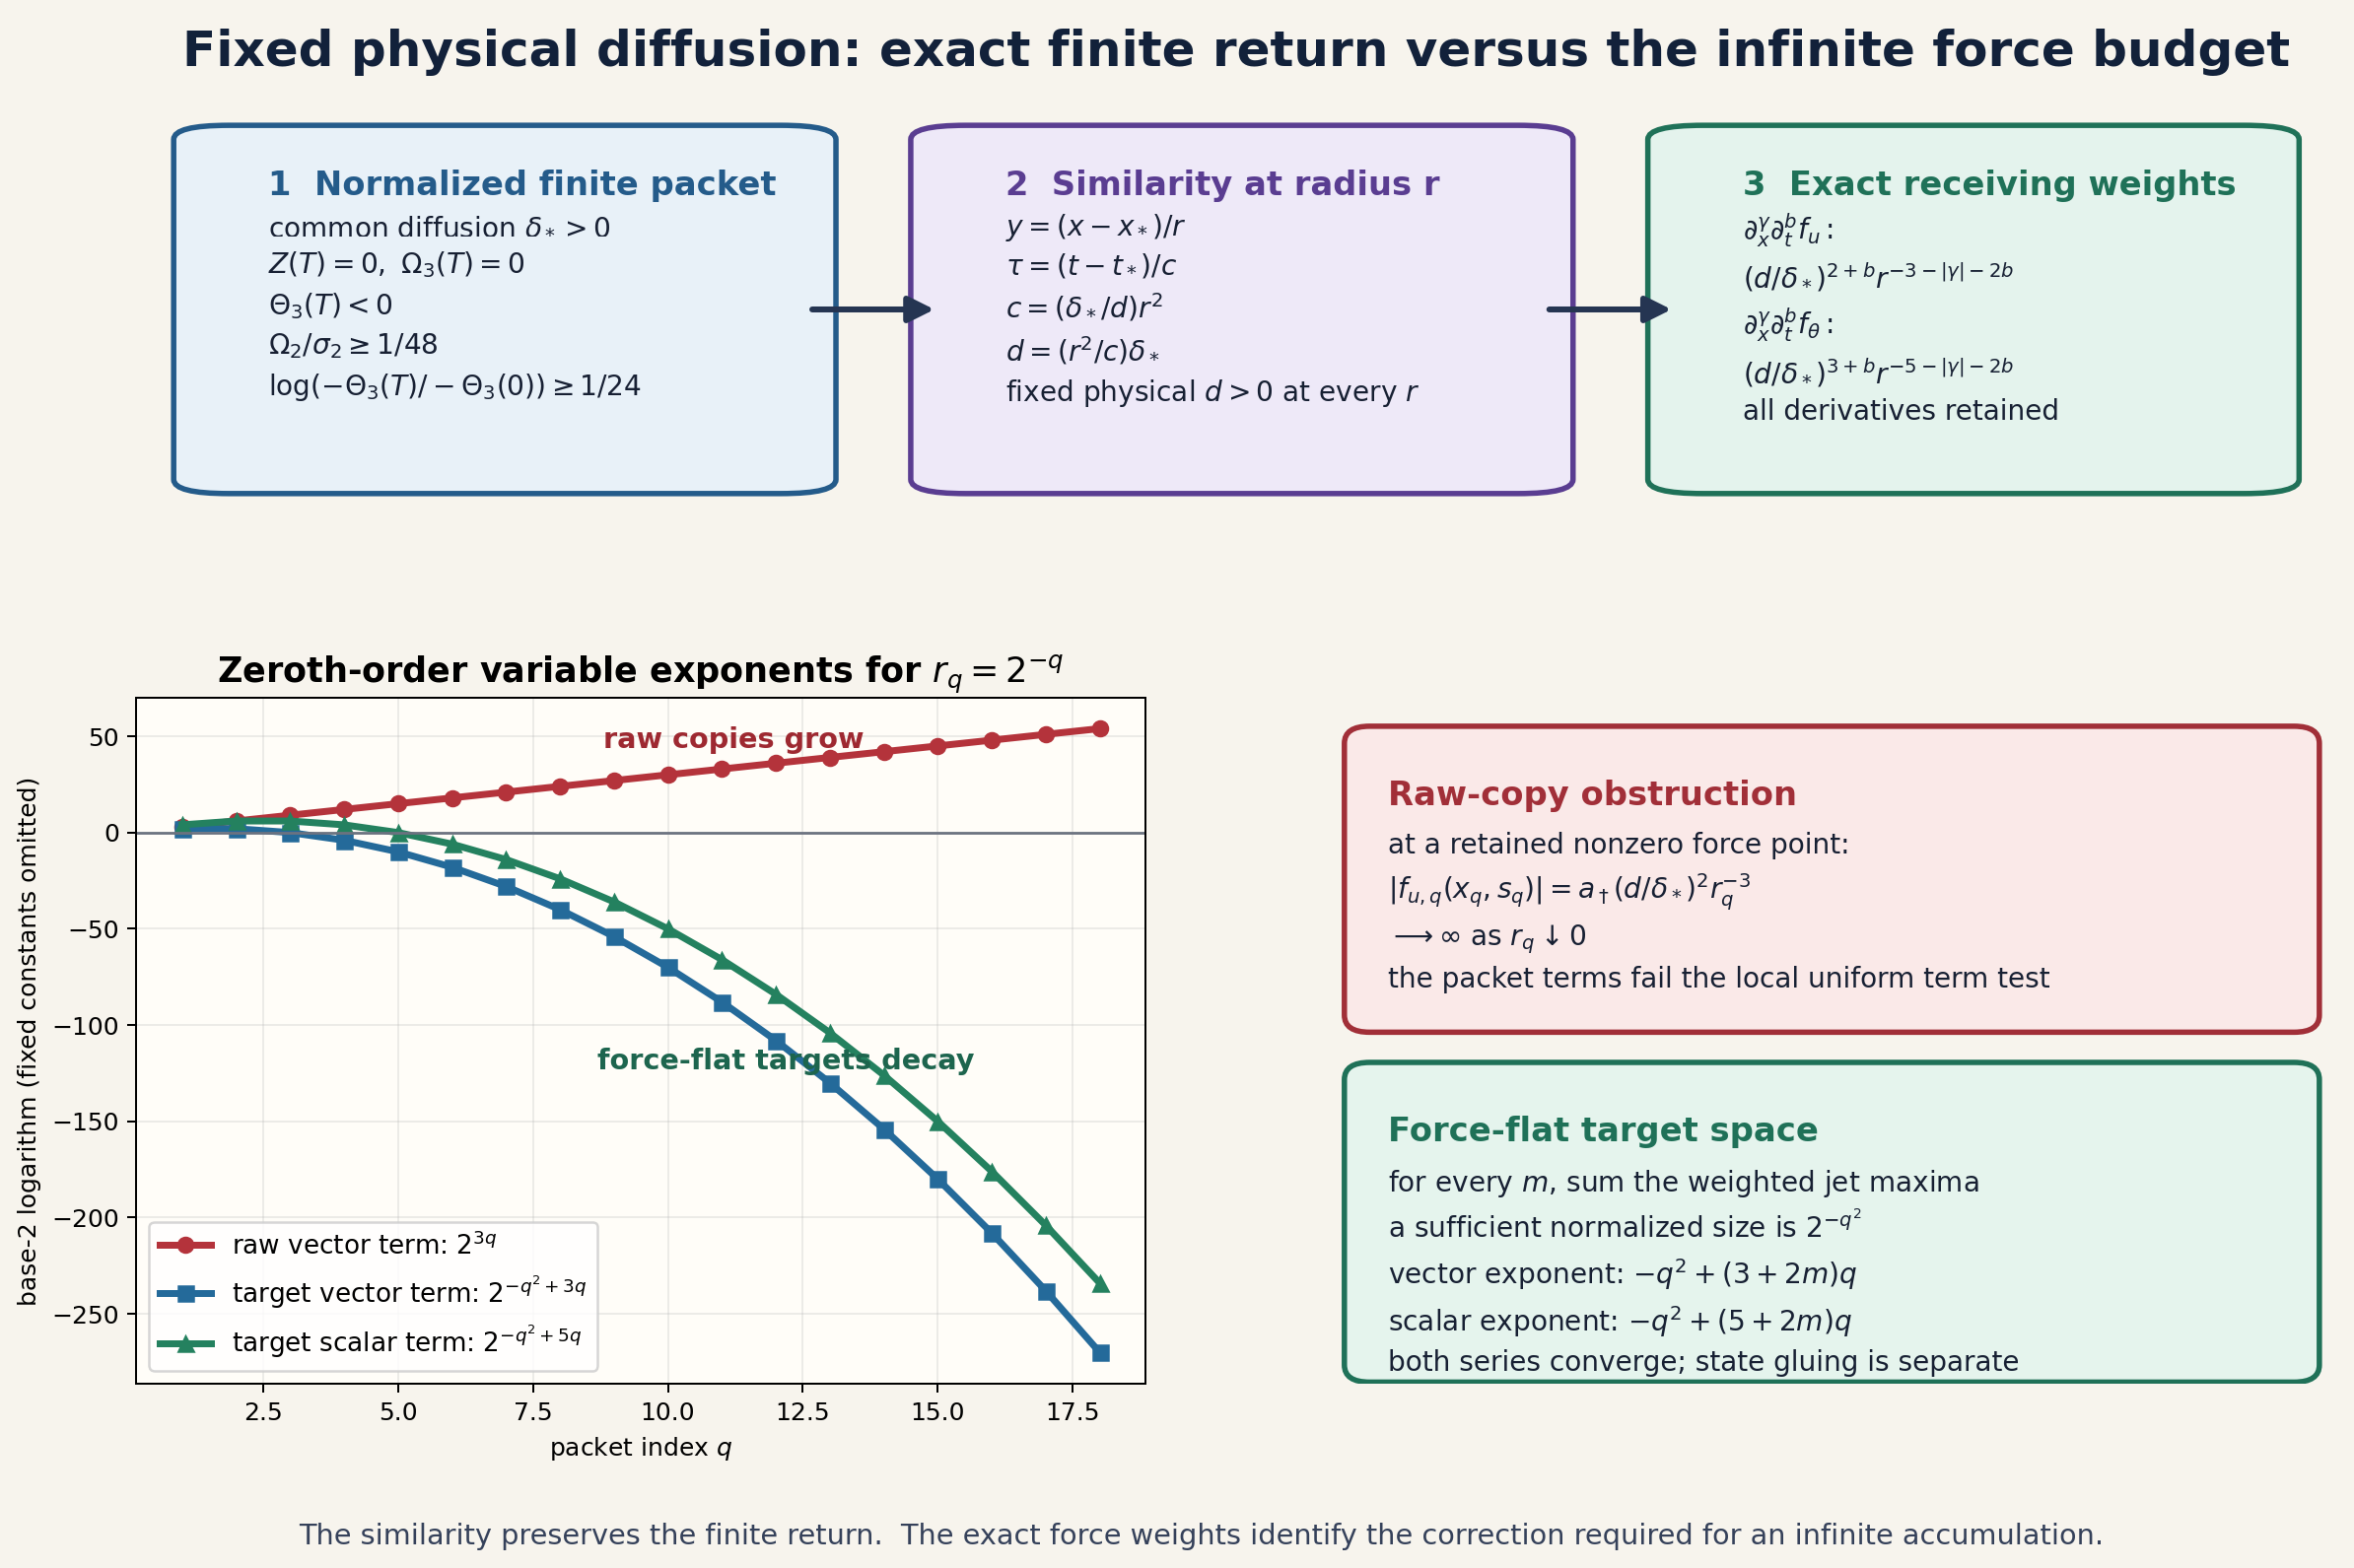
\includegraphics[width=0.96\linewidth]
 {infinite_modified/figures/fixed_diffusion_similarity.png}
 \caption{The fixed-diffusion similarity window.  Parabolic scaling
 transfers the complete finite return to every radius, while the exact
 force-jet powers show that raw copies fail the local uniform term test.
 The force-flat weights are the receiving space for the still-required
 correction and gluing operations.}
 \label{im:fig:similarity}
\end{figure}

\section{The based cascade: exact residual array and state interface}
\label{ibc:section}

The preceding similarity theorem concerns isolated complete packets.  An
infinite construction cannot be obtained by putting one complete packet after
another.  This section proves the state obstruction, replaces packet reset by
an increment over the retained parent, and calculates the complete normalized
residual of that increment.  The calculation keeps the parent velocity,
velocity gradient, temperature gradient, pressure, buoyancy, diffusion, and
every space-time derivative.

\subsection{A complete packet cannot be reset at the next scale}

The stationary left extension of the complete finite packet has $u=0$.
Hence its vorticity and its origin curl are zero.  At the selected third
return, \eqref{trc:diffusive-root-bounds} gives
\begin{equation}\label{ibc:positive-output-curl}
 2\dot\alpha(T)+\Omega_1(T)+\Omega_2(T)
 \geq \frac{c_W}{4}\sigma_2>0.
\end{equation}
The third vorticity is zero there, so this is the full origin curl of the
three-layer returned state.

\begin{proposition}\label{ibc:reset-obstruction}
No two similarity images of the complete finite packet can be joined in
$C^1$ by identifying the returned endpoint of the first with the stationary
initial endpoint of the second.  This holds for every pair of positive radii,
every pair of positive clocks, and every choice of spatial centre.
\end{proposition}

\begin{proof}
Similarity multiplies vorticity by the positive factor $c^{-1}$, by
\eqref{im:vorticity-scale}.  Thus the returned packet has origin curl at
least $c^{-1}c_W\sigma_2/4>0$.  The stationary initial state of every
complete packet has zero velocity everywhere and therefore zero curl at
every possible centre.  Equality of the first spatial derivatives at a join
would imply equality of their curls.  The strict inequality rules this out.
\end{proof}

The obstruction concerns reset.  The returned state can instead be retained
as the parent of a new increment.  A based cascade performs exactly that
retention.

\subsection{Increment over the full retained parent}

Let $(\theta^{<q},u^{<q},p^{<q})$ solve the equal-diffusion Boussinesq
system with physical diffusion $d>0$ and force
$(f_\theta^{<q},f_u^{<q})$.  Let
$(\vartheta_q,v_q,\pi_q)$ be a smooth increment with
$\operatorname{div}v_q=0$, and set
\begin{equation}\label{ibc:cumulative-state}
 \theta^{[q]}=\theta^{<q}+\vartheta_q,\qquad
 u^{[q]}=u^{<q}+v_q,\qquad
 p^{[q]}=p^{<q}+\pi_q.
\end{equation}

\begin{proposition}\label{ibc:physical-residual}
The state \eqref{ibc:cumulative-state} solves the same equation with force
$(f_\theta^{<q}+e_{\theta,q},f_u^{<q}+e_{u,q})$, where
\begin{align}
 e_{\theta,q}={}&\partial_t\vartheta_q
  +u^{<q}\!\cdot\nabla\vartheta_q
  +v_q\!\cdot\nabla\theta^{<q}
  +v_q\!\cdot\nabla\vartheta_q-d\Delta\vartheta_q,
 \label{ibc:scalar-residual}\\
 e_{u,q}={}&\partial_tv_q+(u^{<q}\!\cdot\nabla)v_q
 +(v_q\!\cdot\nabla)u^{<q}+(v_q\!\cdot\nabla)v_q
 +\nabla\pi_q-d\Delta v_q-\vartheta_qe_2.
 \label{ibc:vector-residual}
\end{align}
\end{proposition}

\begin{proof}
Insert \eqref{ibc:cumulative-state} into both Boussinesq equations.
Subtract the two equations for the parent.  Bilinearity gives the three
displayed transport terms in each row, pressure is additive, diffusion is
linear, and the buoyancy difference is $\vartheta_qe_2$.  Moving that
buoyancy difference to the force side gives the last sign in
\eqref{ibc:vector-residual}.  No parent term remains unlisted.
\end{proof}

Inside the finite construction, each newly activated controlled layer is
multiplied by a switching factor that is flat and zero at its left endpoint.
A future based correction must retain this property for its relative
increment.  The switching factor supplies smooth birth of that increment; it
does not supply the state match calculated below.  Keeping every completed
increment in the parent avoids the reset in
Proposition~\ref{ibc:reset-obstruction}.

\subsection{The normalized parent and the exact scaled residual}

Fix a packet centre $(x_q,t_q)$, radius $\rho_q>0$, and
\begin{equation}\label{ibc:clock}
 c_q=\frac{\delta_*}{d}\rho_q^2,\qquad
 y=\frac{x-x_q}{\rho_q},\qquad
 \tau=\frac{t-t_q}{c_q}.
\end{equation}
Write the increment with the complete similarity weights
\begin{equation}\label{ibc:increment-map}
 \vartheta_q=\frac{\rho_q}{c_q^2}\widetilde\vartheta_q,\qquad
 v_q=\frac{\rho_q}{c_q}\widetilde v_q,\qquad
 \pi_q=\frac{\rho_q^2}{c_q^2}\widetilde\pi_q.
\end{equation}
All tilde fields in this section are evaluated at $(y,\tau)$.  Evaluate the
parent at $(x_q+\rho_qy,t_q+c_q\tau)$ and define
\begin{equation}\label{ibc:parent-map}
 \mathcal U_q=\frac{c_q}{\rho_q}u^{<q},\qquad
 \mathcal D_q=c_q\nabla_xu^{<q},\qquad
 \mathcal G_q=c_q^2\nabla_x\theta^{<q}.
\end{equation}

\begin{proposition}\label{ibc:normalized-residual}
The physical residual increments have the exact form
\begin{equation}\label{ibc:residual-scaling}
 e_{\theta,q}=\frac{\rho_q}{c_q^3}\widetilde e_{\theta,q},
 \qquad
 e_{u,q}=\frac{\rho_q}{c_q^2}\widetilde e_{u,q},
\end{equation}
where
\begin{align}
 \widetilde e_{\theta,q}={}&
 \partial_\tau\widetilde\vartheta_q
 +(\mathcal U_q+\widetilde v_q)\cdot
       \nabla_y\widetilde\vartheta_q
 +\widetilde v_q\cdot\mathcal G_q
 -\delta_*\Delta_y\widetilde\vartheta_q,
 \label{ibc:normalized-scalar}\\
 \widetilde e_{u,q}={}&
 \partial_\tau\widetilde v_q
 +(\mathcal U_q+\widetilde v_q)\cdot\nabla_y\widetilde v_q
 +\mathcal D_q\widetilde v_q+\nabla_y\widetilde\pi_q
 -\delta_*\Delta_y\widetilde v_q
 -\widetilde\vartheta_qe_2.
 \label{ibc:normalized-vector}
\end{align}
Consequently every physical residual jet has exactly the force weights
\eqref{im:force-powers}.
\end{proposition}

\begin{proof}
The time, self-transport, pressure, diffusion, and buoyancy terms have the
common factors already proved in Proposition~\ref{im:similarity}.  For the
parent scalar terms,
\[
 u^{<q}\cdot\nabla_x\vartheta_q
 =\frac{\rho_q}{c_q^3}\mathcal U_q\cdot
       \nabla_y\widetilde\vartheta_q,\qquad
 v_q\cdot\nabla_x\theta^{<q}
 =\frac{\rho_q}{c_q^3}\widetilde v_q\cdot\mathcal G_q.
\]
For momentum,
\[
 (u^{<q}\cdot\nabla_x)v_q
 =\frac{\rho_q}{c_q^2}(\mathcal U_q\cdot\nabla_y)
       \widetilde v_q,\qquad
 (v_q\cdot\nabla_x)u^{<q}
 =\frac{\rho_q}{c_q^2}\mathcal D_q\widetilde v_q.
\]
Substitution proves \eqref{ibc:residual-scaling}--
\eqref{ibc:normalized-vector}.  Differentiating
\eqref{ibc:residual-scaling} gives the last assertion with every space and
time factor retained.
\end{proof}

\subsection{All-order residual arrays}

Let $\alpha=(\gamma_1,\gamma_2,b)\in\mathbb N_0^3$, write
$\partial^\alpha=\partial_{y_1}^{\gamma_1}
\partial_{y_2}^{\gamma_2}\partial_\tau^b$, and define
\[
 \binom\alpha\beta=\prod_{j=1}^3\binom{\alpha_j}{\beta_j},
 \qquad
 (A\star B)_\alpha=\sum_{\beta\leq\alpha}
       \binom\alpha\beta A_\beta B_{\alpha-\beta}.
\]
Let $S_1,S_2,S_t$ shift the corresponding derivative index by one.
Write $S_i^2=S_i\circ S_i$ for the twofold spatial shift.
On the complete normalized support and time interval, set
\begin{align*}
 \mathsf T_\alpha&=\|\partial^\alpha\widetilde\vartheta_q\|_\infty,
 &\mathsf V_{i,\alpha}&=\|\partial^\alpha\widetilde v_{q,i}\|_\infty,
 &\mathsf P_\alpha&=\|\partial^\alpha\widetilde\pi_q\|_\infty,\\
 \mathsf U_{i,\alpha}&=\|\partial^\alpha\mathcal U_{q,i}\|_\infty,
 &\mathsf D_{ki,\alpha}&=\|\partial^\alpha\mathcal D_{q,ki}\|_\infty,
 &\mathsf G_{i,\alpha}&=\|\partial^\alpha\mathcal G_{q,i}\|_\infty.
\end{align*}
Repeated Leibniz differentiation of
\eqref{ibc:normalized-scalar}--\eqref{ibc:normalized-vector} gives the
complete finite majorants
\begin{align}
 \mathsf E^\theta={}&S_t\mathsf T
 +\sum_{i=1}^2(\mathsf U_i+\mathsf V_i)\star S_i\mathsf T
 +\sum_{i=1}^2\mathsf V_i\star\mathsf G_i
 +\delta_*\sum_{i=1}^2S_i^2\mathsf T,
 \label{ibc:scalar-array}\\
 \mathsf E^u_k={}&S_t\mathsf V_k
 +\sum_{i=1}^2(\mathsf U_i+\mathsf V_i)\star S_i\mathsf V_k
 +\sum_{i=1}^2\mathsf D_{ki}\star\mathsf V_i
 +S_k\mathsf P+\delta_*\sum_{i=1}^2S_i^2\mathsf V_k
 +\mathbf1_{k=2}\mathsf T.
 \label{ibc:vector-array}
\end{align}
Thus
\begin{equation}\label{ibc:array-bound}
 \|\partial^\alpha\widetilde e_{\theta,q}\|_\infty
 \leq\mathsf E^\theta_\alpha,\qquad
 \|\partial^\alpha\widetilde e_{u,q,k}\|_\infty
 \leq\mathsf E^u_{k,\alpha}.
\end{equation}
Every parent cross term and every self-interaction appears in these arrays.
These are unsigned majorants, not the signed residual itself.  They give
sufficient estimates but may lose exact pressure, buoyancy, and transport
cancellations.  The correction cycle must reduce the actual residual jets;
a norm of the new field alone is not a force estimate.  The exact signed
array and the failure of a necessary unsigned target are proved in
Section~\ref{irc:section}.

For reference, the parent jets in \eqref{ibc:parent-map} are exactly
\begin{align}
 \partial_y^\gamma\partial_\tau^b\mathcal U_q
 &=\rho_q^{|\gamma|-1}c_q^{b+1}
   (\partial_x^\gamma\partial_t^bu^{<q}),
 \label{ibc:parent-u-jets}\\
 \partial_y^\gamma\partial_\tau^b\mathcal D_q
 &=\rho_q^{|\gamma|}c_q^{b+1}
   (\partial_x^\gamma\partial_t^b\nabla_xu^{<q}),
 \label{ibc:parent-d-jets}\\
 \partial_y^\gamma\partial_\tau^b\mathcal G_q
 &=\rho_q^{|\gamma|}c_q^{b+2}
   (\partial_x^\gamma\partial_t^b\nabla_x\theta^{<q}).
 \label{ibc:parent-g-jets}
\end{align}
With $c_q=(\delta_*/d)\rho_q^2$, their radius powers are respectively
\begin{equation}\label{ibc:parent-radius-powers}
 \rho_q^{|\gamma|+2b+1},\qquad
 \rho_q^{|\gamma|+2b+2},\qquad
 \rho_q^{|\gamma|+2b+4},
\end{equation}
times the displayed fixed powers of $\delta_*/d$ and the corresponding
physical parent derivatives.

\subsection{The state-renormalization equation}

The positive powers in \eqref{ibc:parent-radius-powers} do not permit one
to discard the parent.  The return mechanism requires a nonzero normalized
temperature gradient and a specified normalized velocity gradient.  The
normalized entry profile carried by the retained parent is, by definition,
the triple $(\mathcal U_q,\mathcal D_q,\mathcal G_q)$ in
\eqref{ibc:parent-map}.  For a prescribed next-stage profile
$(\mathcal U_q^{\rm in},\mathcal D_q^{\rm in},
\mathcal G_q^{\rm in})$, equality with that profile is equivalent to the
three exact inverse equations
\begin{equation}\label{ibc:state-interface}
 \begin{aligned}
 u^{<q}(x_q+\rho_qy,t_q+c_q\tau)
    &=\frac{\rho_q}{c_q}\mathcal U_q^{\rm in}(y,\tau),\\
 \nabla_xu^{<q}(x_q+\rho_qy,t_q+c_q\tau)
    &=c_q^{-1}\mathcal D_q^{\rm in}(y,\tau),\\
 \nabla_x\theta^{<q}(x_q+\rho_qy,t_q+c_q\tau)
    &=c_q^{-2}\mathcal G_q^{\rm in}(y,\tau)
 \end{aligned}
\end{equation}
on the required normalized space-time support.  If a proved next-stage entry
set contains more than one such profile, admissibility means that the actual
triple from \eqref{ibc:parent-map} belongs to that set; the inverse equations
remain exact for the profile it realizes.  At the centre, the three physical
scale factors are
\begin{equation}\label{ibc:state-powers}
 \frac d{\delta_*}\rho_q^{-1},\qquad
 \frac d{\delta_*}\rho_q^{-2},\qquad
 \left(\frac d{\delta_*}\right)^2\rho_q^{-4}.
\end{equation}
A parent with uniformly bounded first derivatives tends to zero in the last
two normalized coordinates and cannot reproduce a fixed nonzero entry tuple.
Reproduction of fixed nonzero gradient entries requires the precise
$\rho_q^{-2}$ velocity-gradient and $\rho_q^{-4}$ temperature-gradient
growth encoded by \eqref{ibc:state-interface}.

Equation \eqref{ibc:state-interface} is vector- and matrix-valued.  Choosing
$\rho_q$ from a single norm does not prove it: directions, signs, phase
lengths, parent amplitudes, and every derivative required by
\eqref{ibc:scalar-array}--\eqref{ibc:vector-array} must also match.  The
third-return theorem proves the strict output signs and bounds
\eqref{trc:diffusive-root-bounds}; it does not yet prove that its complete
output, after one dilation, lies in a valid fourth-stage entry set.

This answers the next-step question exactly.  A successful infinite
construction needs a based return-renormalization map satisfying
\eqref{ibc:state-interface}, together with corrections that place the
actual signed residuals \eqref{ibc:normalized-scalar}--
\eqref{ibc:normalized-vector} in the force-flat bounds
\eqref{im:flat-u}--\eqref{im:flat-theta}.  For the concrete choice
$\rho_q=2^{-q}$, bounds
\begin{equation}\label{ibc:target-array}
 \max_{|\alpha|\leq q}
   \|\partial^\alpha\widetilde e_{\theta,q}\|_\infty\leq2^{-q^2},
 \qquad
 \max_{k\in\{1,2\},\ |\alpha|\leq q}
   \|\partial^\alpha\widetilde e_{u,q,k}\|_\infty\leq2^{-q^2}
\end{equation}
are sufficient by the summability calculation following
\eqref{im:explicit-budget}.  The stronger bounds with $\mathsf E$ in
place of the displayed norms are also sufficient, but are not required.
Neither bound is asserted for the present finite packet.  The
complete-copy construction fails
Proposition~\ref{ibc:reset-obstruction}; the based residual and state maps
above are the exact objects that replace it.

The similarity factors, parent-jet powers, residual terms, and convolution
indices are replayed in
\texttt{infinite\_modified/checks/based\_cascade\_check.py}.  Figure~
\ref{ibc:fig:based-cascade} shows the state and force interfaces together.

\begin{figure}[htbp]
 \centering
 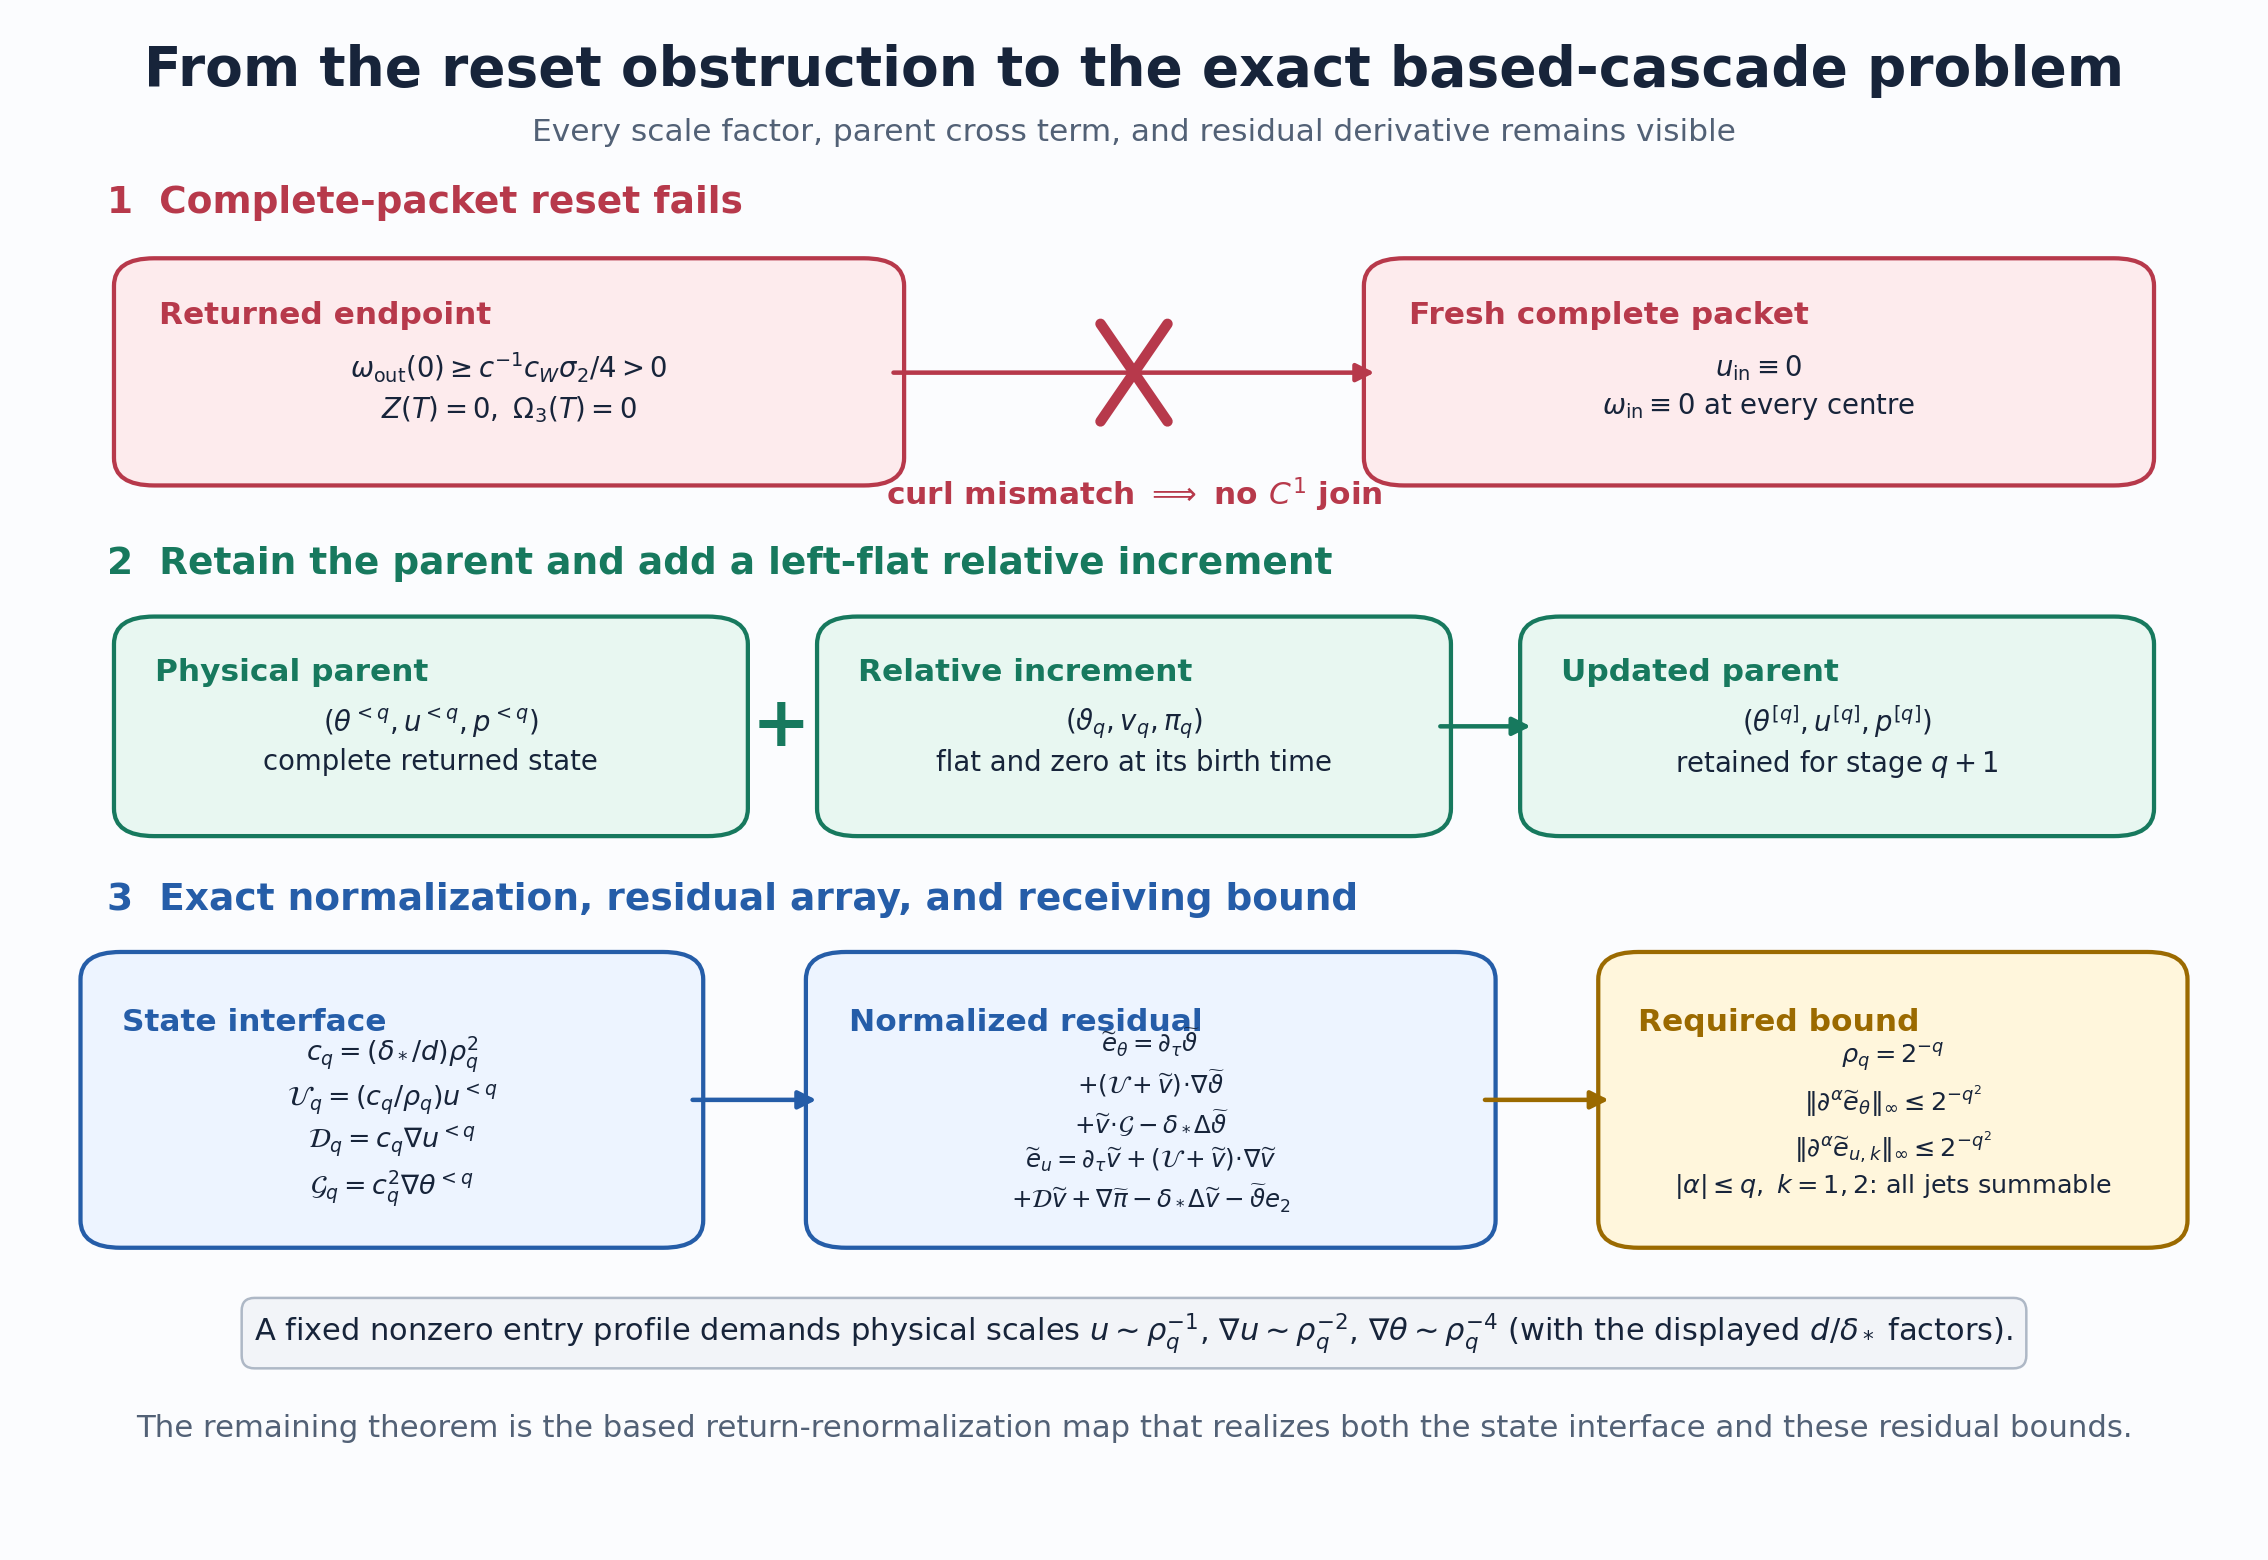
\includegraphics[width=0.96\linewidth]
 {infinite_modified/figures/based_cascade_residual.png}
 \caption{Complete packets fail at the state join because returned curl is
 positive while every reset packet starts with zero curl.  A based cascade
 retains the returned parent, rescales its complete velocity and temperature
 jets through \eqref{ibc:state-interface}, and corrects the exact incremental
 signed residual into the force-flat receiving space.}
 \label{ibc:fig:based-cascade}
\end{figure}

\section{Signed residuals, the exact returned core, and a compact correction}
\label{irc:section}

This section corrects the unsigned target in the earlier continuation.
It then calculates the complete chart transition and the actual affine
state at the selected third return.  That state supplies an explicit
unforced local continuation.  A flat interpolation and a compact
streamfunction correction connect it to the retained finite field,
with every transition and cutoff contribution displayed.  The
construction is finite and local; its force cost is not claimed to
satisfy an infinite-stage budget.

\subsection{The signed force jets and the unsigned-target defect}

Use the three-index notation of Section~\ref{ibc:section}.  In this
subsection only, write $T_\alpha=\partial^\alpha\widetilde\vartheta$,
$V_{i,\alpha}=\partial^\alpha\widetilde v_i$,
$P_\alpha=\partial^\alpha\widetilde\pi$,
$U_{i,\alpha}=\partial^\alpha\mathcal U_i$,
$D_{ki,\alpha}=\partial^\alpha\mathcal D_{ki}$ and
$G_{i,\alpha}=\partial^\alpha\mathcal G_i$.
These are signed functions, with no norm taken.  Let $e_1,e_2,e_t$
denote index shifts, distinct from the physical vector $e_2=(0,1)$.
Repeated differentiation gives the exact signed arrays
\begin{align}
 R^\theta_\alpha={}&T_{\alpha+e_t}
 +\sum_{i=1}^2\sum_{\beta\leq\alpha}\binom\alpha\beta
 \left[(U_{i,\beta}+V_{i,\beta})T_{\alpha-\beta+e_i}
       +V_{i,\beta}G_{i,\alpha-\beta}\right]
 -\delta_*\sum_{i=1}^2T_{\alpha+2e_i},
 \label{irc:signed-scalar}\\
 R^u_{k,\alpha}={}&V_{k,\alpha+e_t}
 +\sum_{i=1}^2\sum_{\beta\leq\alpha}\binom\alpha\beta
 \left[(U_{i,\beta}+V_{i,\beta})V_{k,\alpha-\beta+e_i}
       +D_{ki,\beta}V_{i,\alpha-\beta}\right]\nonumber\\
 &+P_{\alpha+e_k}-\delta_*\sum_{i=1}^2V_{k,\alpha+2e_i}
       -\mathbf1_{k=2}T_\alpha.
 \label{irc:signed-vector}
\end{align}
They equal $\partial^\alpha\widetilde e_\theta$ and
$\partial^\alpha\widetilde e_{u,k}$, respectively, by the product
rule.  Applying the triangle inequality after these equalities gives
\eqref{ibc:scalar-array}--\eqref{ibc:array-bound}.

\begin{proposition}\label{irc:unsigned-defect}
The unsigned majorants are not necessary force bounds.  On the closed
unit ball, the exact fields
\[
 \widetilde\vartheta(y,\tau)=y_2,\qquad
 \widetilde v=0,\qquad \widetilde\pi=y_2^2/2,\qquad
 \mathcal U=\mathcal D=\mathcal G=0
\]
have identically zero scalar and vector residuals for every
$\delta_*>0$, whereas $\mathsf E^u_{2,0}=2$.
Furthermore, on a duration-$L$ cylinder, bounds
$\max_k\mathsf E^u_{k,0}\leq\epsilon$ imply
$\|\widetilde\vartheta\|_\infty\leq\epsilon$ and, for an increment
starting at $\widetilde v(\cdot,0)=0$,
$\|\widetilde v_k(\cdot,L)\|_\infty\leq L\epsilon$.
\end{proposition}

\begin{proof}
Here $\nabla\widetilde\pi=y_2e_2=\widetilde\vartheta e_2$,
$\Delta\widetilde\vartheta=0$, and every velocity term is zero.
The signed residuals therefore vanish.  The unsigned second momentum
row contains $\|\partial_2\widetilde\pi\|_\infty+
\|\widetilde\vartheta\|_\infty=1+1$, with all its other terms zero.
For the second assertion, all summands in $\mathsf E$ are nonnegative.
Its second momentum row contains $\mathsf T_0$, and each momentum row
contains $\|\partial_\tau\widetilde v_k\|_\infty$.  Integration from
zero to $L$ proves the asserted endpoint bound.  Thus requiring these
majorants to tend to zero on uniformly bounded durations excludes
increments with a fixed nonzero temperature or velocity amplitude,
even when their actual force cancels.  The example is local and
noncompact; it is not asserted to be a compact packet.
\end{proof}

Consequently \eqref{ibc:target-array} now refers to the norms of
\eqref{irc:signed-scalar}--\eqref{irc:signed-vector}.  The old
unsigned target is retained only as a sufficient estimate, with its
earlier source version preserved in the main's provenance directory.

\subsection{Exact receiving map for a correction}

Let $\mathcal B=(c_q^2/\rho_q)\theta^{<q}$ and
$\mathcal P=(c_q^2/\rho_q^2)p^{<q}$ in the same chart.  Thus
$\nabla\mathcal B=\mathcal G$ and $\nabla\mathcal U=\mathcal D$.
Set
\[
 \mathcal T=\mathcal B+\widetilde\vartheta,\qquad
 \mathcal V=\mathcal U+\widetilde v.
\]
For a correction $(h,z,\kappa)$ with $\operatorname{div}z=0$, replace
$(\widetilde\vartheta,\widetilde v,\widetilde\pi)$ by
$(\widetilde\vartheta+h,\widetilde v+z,\widetilde\pi+\kappa)$.
Subtraction of the complete equations gives
\begin{align}
 \Delta\widetilde e_\theta={}&
 h_\tau+\mathcal V\cdot\nabla h+z\cdot\nabla\mathcal T
 +z\cdot\nabla h-\delta_*\Delta h,
 \label{irc:correction-scalar}\\
 \Delta\widetilde e_u={}&
 z_\tau+(\mathcal V\cdot\nabla)z+(z\cdot\nabla)\mathcal V
 +(z\cdot\nabla)z+\nabla\kappa-\delta_*\Delta z-he_2.
 \label{irc:correction-vector}
\end{align}
Every jet of the updated residual is obtained by differentiating
these identities and adding it to the old signed jet.  In particular,
the correction equation is an equation for the actual signed
functions, before any majorant is introduced.  These formulas also
prove the compatibility constraints on a proposed entry tuple:
$\mathcal D=\nabla\mathcal U$, $\mathcal G=\nabla\mathcal B$,
$\operatorname{tr}\mathcal D=0$, and
$\partial_1\mathcal G_2=\partial_2\mathcal G_1$.
They follow by direct differentiation of the defined pullbacks;
three independently chosen arrays need not be a realizable tuple.

\subsection{The complete chart transition}

Keep the physical $d>0$ and $\delta_*>0$ fixed.  Let two charts have
radii $\rho,\rho'>0$, clocks $c=(\delta_*/d)\rho^2$ and
$c'=(\delta_*/d)(\rho')^2$, and centres $(x_0,t_0)$ and
$(x'_0,t'_0)$.  Define
\[
 a=\rho'/\rho>0,\qquad
 \xi=(x'_0-x_0)/\rho,\qquad \tau_0=(t'_0-t_0)/c.
\]
Write $(\Theta,U,P)$ for the complete scalar, velocity and pressure
pullbacks in the first chart, including every retained layer and
cutoff.  The second chart is exactly
\begin{equation}\label{irc:full-chart}
 \begin{aligned}
 \Theta'(y,s)&=a^3\Theta(\xi+ay,\tau_0+a^2s),\\
 U'(y,s)&=aU(\xi+ay,\tau_0+a^2s),\\
 P'(y,s)&=a^2P(\xi+ay,\tau_0+a^2s).
 \end{aligned}
\end{equation}
This follows from the ratios $c'^2/\rho'$ to $c^2/\rho$,
$c'/\rho'$ to $c/\rho$, and $c'^2/(\rho')^2$ to $c^2/\rho^2$.
It proves, with every argument retained,
\begin{equation}\label{irc:gradient-chart}
 D'=a^2D(\xi+ay,\tau_0+a^2s),\qquad
 G'=a^4G(\xi+ay,\tau_0+a^2s).
\end{equation}
Space-time jets of $\Theta,U,P$ acquire respectively
$a^{3+|\gamma|+2b}$, $a^{1+|\gamma|+2b}$ and
$a^{2+|\gamma|+2b}$; those of $D,G$ acquire
$a^{2+|\gamma|+2b}$ and $a^{4+|\gamma|+2b}$.
The complete scalar and vector forces acquire
$a^{5+|\gamma|+2b}$ and $a^{3+|\gamma|+2b}$.
The chain rule proves each identity; no periodic argument, support
boundary, pressure contribution or older layer is replaced.
The inverse uses $a^{-1}$, $-\xi/a$, and $-\tau_0/a^2$.

For a centred affine snapshot $U(y)=Dy$, $\Theta(y)=G\cdot y$,
the action becomes $(D,G)\mapsto(a^2D,a^4G)$.

\begin{proposition}\label{irc:orbit-classification}
On the exact state space
$\{(D,G):D\in\mathbb R^{2\times2},\operatorname{tr}D=0,\,
G\in\mathbb R^2\setminus\{0\}\}$, two centred affine snapshots are
related by a positive parabolic dilation precisely when
\begin{equation}\label{irc:complete-invariants}
 \frac{G'}{|G'|}=\frac G{|G|},\qquad
 \frac{D'}{\sqrt{|G'|}}=\frac D{\sqrt{|G|}}.
\end{equation}
The radius ratio is then uniquely
$a=(|G'|/|G|)^{1/4}$.  It is a shrinking dilation precisely when
$|G'|<|G|$.
\end{proposition}

\begin{proof}
The action in \eqref{irc:gradient-chart} preserves both displayed
quantities since $a>0$.  Conversely, their equality and the displayed
choice of $a$ give $G'=a^4G$ and $D'=a^2D$ entry by entry.
This proves the full orbit classification, including the direction
and every matrix entry.  For curl $W=D_{21}-D_{12}$ it also gives the
invariant $W/\sqrt{|G|}$.  Thus selection of a radius from $|G|$
cannot change the remaining state coordinates.
\end{proof}

\subsection{The actual third-return affine state}

At the selected return time $t_R$, retain all original constants and
the determinant coordinates of \eqref{tr:coordinates}.  In the
following display $D_{\rm ph}=h^2+a_{\rm ph}^2$ is the source scalar
$D$; $a_{\rm ph}=\sin s_2$ distinguishes it from a radius ratio.
The other source names $b,x,y,g,R,c=A_0\cos s_*$ and
$C=A_0\sin s_*$ are unchanged.  On a common affine neighbourhood,
the full physical fields are
\begin{equation}\label{irc:return-field}
 \theta=G_R\cdot x,\qquad u=\mathcal A_Rx,\qquad p=0,
\end{equation}
where
\begin{align}
 G_R&=-A_0R_\alpha e_2+
       \sum_{j=1}^3K_j\Theta_j\zeta_j,
 \label{irc:return-G}\\
 \mathcal A_R&=\dot\alpha J+
       \sum_{j=1}^3\frac{\Omega_j}{|\zeta_j|^2}
                 J\zeta_j\otimes\zeta_j.
 \label{irc:return-D}
\end{align}
These are restrictions of the complete periodic-profile and
material-cutoff fields, rather than new definitions of those fields.
Indeed $F(s)=s$ on $|s|<s_0$, $P'(s)=F(s)$, and every material cutoff
equals one in a neighbourhood of the origin.  The sums therefore
give exactly their scalar and streamfunction derivatives there.

The return and hold equations give
$\zeta_3=(0,\sqrt R)$, $\Omega_3=0$,
$\zeta_1=(-y,x)/\sqrt R$, and $\zeta_2=(-b,g)/\sqrt R$.
Since $\dot\zeta_{3,1}=0$ on the hold and
$\dot\zeta_3=-D_{<3}^T\zeta_3$, one has
$(D_{<3})_{21}=0$.  At the endpoint it follows also by substitution
of the displayed angular control in \eqref{tr:hold}.  Tracelessness
and \eqref{trc:diffusive-root-bounds} yield
\begin{equation}\label{irc:triangular-return}
 \mathcal A_R=
 \begin{pmatrix}a_R&-W_R\\0&-a_R\end{pmatrix},\qquad
 a_R=\frac{\Omega_1xy}{R}
       +\frac{\Omega_2bg}{D_{\rm ph}R},\qquad
 W_R=2\dot\alpha+\Omega_1+\Omega_2
       \geq c_W\sigma_2/4>0.
\end{equation}
No strain sign is imposed.  The angular inverse gives
$\alpha=s_*+\arctan(y/x)$ at this endpoint.  Therefore, retaining
the base and all three temperature terms,
\begin{equation}\label{irc:exact-return-temperature}
 \begin{aligned}
 (G_R)_1&=\frac{(E_1+c)y+Cx+bE_2}{\sqrt R}
          =\frac{N_3}{\sqrt R}>0,\\
 (G_R)_2&=-\frac{(E_1+c)x-Cy+gE_2}{\sqrt R}
             +K_3\Theta_3\sqrt R.
 \end{aligned}
\end{equation}
Positivity uses the proved positive component $N_3$, not an
unproved sign for $(G_R)_2$.  The nonzero $G_R$ lies in the state
space of Proposition~\ref{irc:orbit-classification}.  At a physical
radius $\rho$ its chart coefficients are exactly
$c_\rho\mathcal A_R$ and $c_\rho^2G_R$; a further radius ratio
multiplies these by $a^2$ and $a^4$.  This preserves all physical
diffusion and clock factors in \eqref{ibc:clock}.

\subsection{An explicit unforced affine continuation}

Put $a=a_R$, $b_0=-W_R$, $g_1=(G_R)_1>0$ and
$g_2=(G_R)_2$, without resetting their values.  For $s=t-t_R$ set
\begin{align}
 \Phi_k(a,s)&=\int_0^s e^{-ka r}\,dr
 =\begin{cases}(1-e^{-ka s})/(ka),&a\ne0,\\s,&a=0,\end{cases}
 \quad k=1,2,3,\nonumber\\
 \Xi(a,s)&=\int_0^s e^{-2ar}\Phi_1(a,r)\,dr
 =\begin{cases}(\Phi_2(a,s)-\Phi_3(a,s))/a,&a\ne0,\\
 s^2/2,&a=0.\end{cases}
 \label{irc:affine-integrals}
\end{align}
Define the complete coefficients
\begin{equation}\label{irc:affine-solution}
 \begin{aligned}
 g_1(s)&=g_1e^{-as},&
 b(s)&=b_0-g_1\Phi_1(a,s),\\
 g_2(s)&=e^{as}\left[g_2-g_1b_0\Phi_2(a,s)
                              +g_1^2\Xi(a,s)\right],&
 A(s)&=\begin{pmatrix}a&b(s)\\0&-a\end{pmatrix},\\
 G(s)&=(g_1(s),g_2(s)),&
 H(s)&=\begin{pmatrix}-a^2&g_1(s)\\g_1(s)&g_2(s)-a^2\end{pmatrix}.
 \end{aligned}
\end{equation}

\begin{theorem}\label{irc:affine-continuation}
For every physical $d>0$, the fields
$\theta_A(x,t)=G(s)\cdot x$, $u_A(x,t)=A(s)x$ and
$p_A(x,t)=x^TH(s)x/2$ solve the unforced equal-diffusion
Boussinesq equations on $\mathbb R^2\times\mathbb R$.
Their temperature and velocity at $t_R$ agree exactly with
\eqref{irc:return-field} on its affine neighbourhood.
For $s\geq0$,
\[
 (\nabla\theta_A)_1=g_1e^{-as}>0,\qquad
 \operatorname{curl}u_A=W_R+g_1\Phi_1(a,s)>0.
\]
All coefficients are finite at every finite $s$.
\end{theorem}

\begin{proof}
The integral formulas, including their $a=0$ values, are smooth
in $a,s$ by their integral definitions.  Differentiation gives
$g_1'=-ag_1(s)$, $b'=-g_1(s)$, and
$g_2'=-b(s)g_1(s)+ag_2(s)$.  Hence
$G'+A^TG=0$.  Direct multiplication retains the full matrix
$A^2=a^2I$ and gives
$A'+A^2+H-e_2G^T=0$.
These two identities are precisely the scalar and momentum
equations; $\Delta(G\cdot x)=0$, $\Delta(Ax)=0$, and
$\operatorname{div}(Ax)=\operatorname{tr}A=0$.
The pressure is symmetric and supplies its displayed gradient.
At $s=0$, $\Phi_k=\Xi=0$, so the temperature and velocity
coefficients are the original ones.  For $s\geq0$,
$\Phi_1\geq0$, which proves both signs.
Exponential and finite integrals prove finiteness at every finite
$s$.  This solution is noncompact.  Its initial pressure need
not equal the old zero pressure, and the equations need not
match the old time jets; the next construction repairs the join.
\end{proof}

\subsection{A flat join with every transition term retained}

The selected finite return has a smooth holding continuation on
some compact interval $I=[t_R,t_R+\epsilon]$: local existence of
its smooth finite vector field and the interior component bounds
prove this.  Denote its affine coefficients by $A_h,G_h,H_h=0$.
They retain the nonstationary temperature diffusion and all older
responses in \eqref{tr:hold}--\eqref{trc:holding}.
Choose $0<\ell<\epsilon$ and $\beta(t)=\eta((t-t_R)/\ell)$.
Set $\Delta A=A-A_h$, $\Delta G=G-G_h$ and $\Delta H=H-H_h$,
and define
\begin{equation}\label{irc:flat-interpolation}
 A_\beta=A_h+\beta\Delta A,\quad
 G_\beta=G_h+\beta\Delta G,\quad
 H_\beta=H_h+\beta\Delta H.
\end{equation}
Let the old affine residual coefficients be
$r_h^\theta=G_h'+A_h^TG_h$ and
$r_h^u=A_h'+A_h^2+H_h-e_2G_h^T$.
The total interpolated core residual is exactly
\begin{align}
 r_\beta^\theta&=(1-\beta)r_h^\theta
             +\beta'\Delta G
             -\beta(1-\beta)(\Delta A)^T\Delta G,
 \label{irc:transition-scalar}\\
 r_\beta^u&=(1-\beta)r_h^u
             +\beta'\Delta A-\beta(1-\beta)(\Delta A)^2.
 \label{irc:transition-vector}
\end{align}
The scalar force is $r_\beta^\theta\cdot x$ and the vector
force is $r_\beta^ux$.  To verify these identities, expand
$A_\beta^TG_\beta$ and $A_\beta^2$ and compare their
quadratic terms with $(1-\beta)$ times the old expression and
$\beta$ times the new zero residual.  The difference is
$-\beta(1-\beta)$ times the two displayed products.  Derivatives
of the interpolation give exactly the $\beta'$ terms.
The pressure and buoyancy are linear and are both retained.
For $t\leq t_R$ the interpolated fields equal the old ones with
every time jet; for $t\geq t_R+\ell$ they equal the explicit
unforced core with every time jet.  Flatness of $\eta$ proves both
joins, including the pressure join.

\subsection{Compact realization over the actual retained parent}

The affine neighbourhood can be chosen uniformly on $I$.
Indeed all phase and material matrix norms have finite maxima there.
Writing $L_j=\sup_I\|M_j^{-1}\|$ and
$Z_j=\sup_I|\zeta_j|$, one possible positive radius is
\[
 r_c=\min\left(1,\frac{s_0}{2\mu},
       \min_{1\leq j\leq3}\frac{\ell_j}{4L_j},
       \min_{1\leq j\leq3}\frac{s_0}{2K_jZ_j}\right).
\]
The unchanged $\ell_j$ are the original material envelope radii.
On $B_{r_c}$ the base and every activated profile are exactly
affine, and every material cutoff is one.  This proves the needed
neighbourhood directly, without extending a local support estimate
to the full third trial family.

Take $\chi\in C_c^\infty(B_{r_c})$ equal to one on
$B_{r_c/2}$.  With $B=-J\beta\Delta A$ symmetric, put
\begin{equation}\label{irc:compact-correction}
 h=\chi\,\beta\Delta G\cdot x,\qquad
 Q=x^TBx/2,\qquad z=J\nabla(\chi Q),\qquad
 \kappa=\chi\,x^T(\beta\Delta H)x/2.
\end{equation}
These are physical fields.  Symmetry of $B$ follows from
$\operatorname{tr}(\beta\Delta A)=0$ by multiplying its four
entries; $J B=\beta\Delta A$.
The correction is compact and divergence free, is flat at birth,
and equals the difference between \eqref{irc:flat-interpolation}
and the held core on $B_{r_c/2}$.

For completeness write $L=\beta\Delta A$, $g=\beta\Delta G$,
$K=\beta\Delta H$, so that $B=-JL$ and $Q=x^TBx/2$.
Its complete first and diffusion derivatives are
\begin{align}
 z&=\chi Lx+QJ\nabla\chi,\nonumber\\
 \nabla z&=\chi L+(Lx)\otimes\nabla\chi
          +(J\nabla\chi)\otimes(Bx)+QJ\nabla^2\chi,
 \label{irc:cutoff-gradient}\\
 \Delta z&=(\Delta\chi)Lx+2L\nabla\chi
          +(\operatorname{tr}B)J\nabla\chi
          +2J(\nabla^2\chi)Bx+QJ\nabla\Delta\chi,
 \label{irc:cutoff-laplacian}\\
 \nabla h&=\chi g+(g\cdot x)\nabla\chi,\qquad
 \Delta h=(g\cdot x)\Delta\chi+2g\cdot\nabla\chi,\nonumber\\
 \nabla\kappa&=\chi Kx+\tfrac12(x^TKx)\nabla\chi,\nonumber\\
 h_t&=\chi g'\cdot x,\qquad
 z_t=\chi L'x+\tfrac12(x^TB'x)J\nabla\chi.
 \label{irc:cutoff-time}
\end{align}
Substituting these fields and derivatives into the physical
identities \eqref{ibc:scalar-residual}--\eqref{ibc:vector-residual}
with the full retained parent gives their exact global force
increment, including both $d\Delta$ terms.  The product rule
gives all higher jets; no derivative of $\chi$ is discarded.

\begin{proposition}\label{irc:compact-core-repair}
The actual held finite field admits the compact smooth based
correction \eqref{irc:compact-correction}.  The resulting fields
have the same complete initial time jets at $t_R$ as the old
finite field.  On $B_{r_c/2}$ their total force is exactly
\eqref{irc:transition-scalar}--\eqref{irc:transition-vector}
during the transition and is zero on
$[t_R+\ell,t_R+\epsilon]$.
Outside $B_{r_c}$ both state and force equal the retained parent's.
\end{proposition}

\begin{proof}
The streamfunction proves $\operatorname{div}z=0$ by equality
of mixed derivatives.  Flatness of $\beta$ proves all initial
jets, including those of the compact pressure.  Where $\chi=1$
the state is exactly the interpolated affine state, so the
proved residual identities apply.  Where $\beta=1$ that state
is the explicit unforced solution.  Outside the compact support
every correction derivative is zero, and the exact physical
increment residual vanishes.  This also proves support and
smoothness of the full added force.
\end{proof}

The zero assertion concerns the \emph{total} core force.
After the transition the force increment there equals the
negative old force; it need not be small.  The transition terms
and cutoff annulus also have no established $2^{-q^2}$ bound.
The operation now constructed is a compact, left-flat state
correction with an exact force map.  The next calculation is to
evaluate that signed force on the full support, including the
annulus, and construct a subsequent return whose complete
profile satisfies \eqref{irc:complete-invariants} or the broader
exact entry equation \eqref{ibc:state-interface}.  The explicit
constant-strain affine solution has no finite-time singularity;
it supplies a correction of the local force, not the missing
infinite blowup construction.

The identities are replayed by \path{return_correction_check.py}
in \path{infinite_modified/checks}.
Figure~\ref{irc:figure} shows the actual state and the full
transition-force decomposition.  The original profiles and
control sums are those of Alp\"oge--Buckmaster, source
Sections~3.3 and 3.7.10 and equations (4.9)--(4.10), retained
with their exact receiving formulas above.

\begin{figure}[htbp]
 \centering
 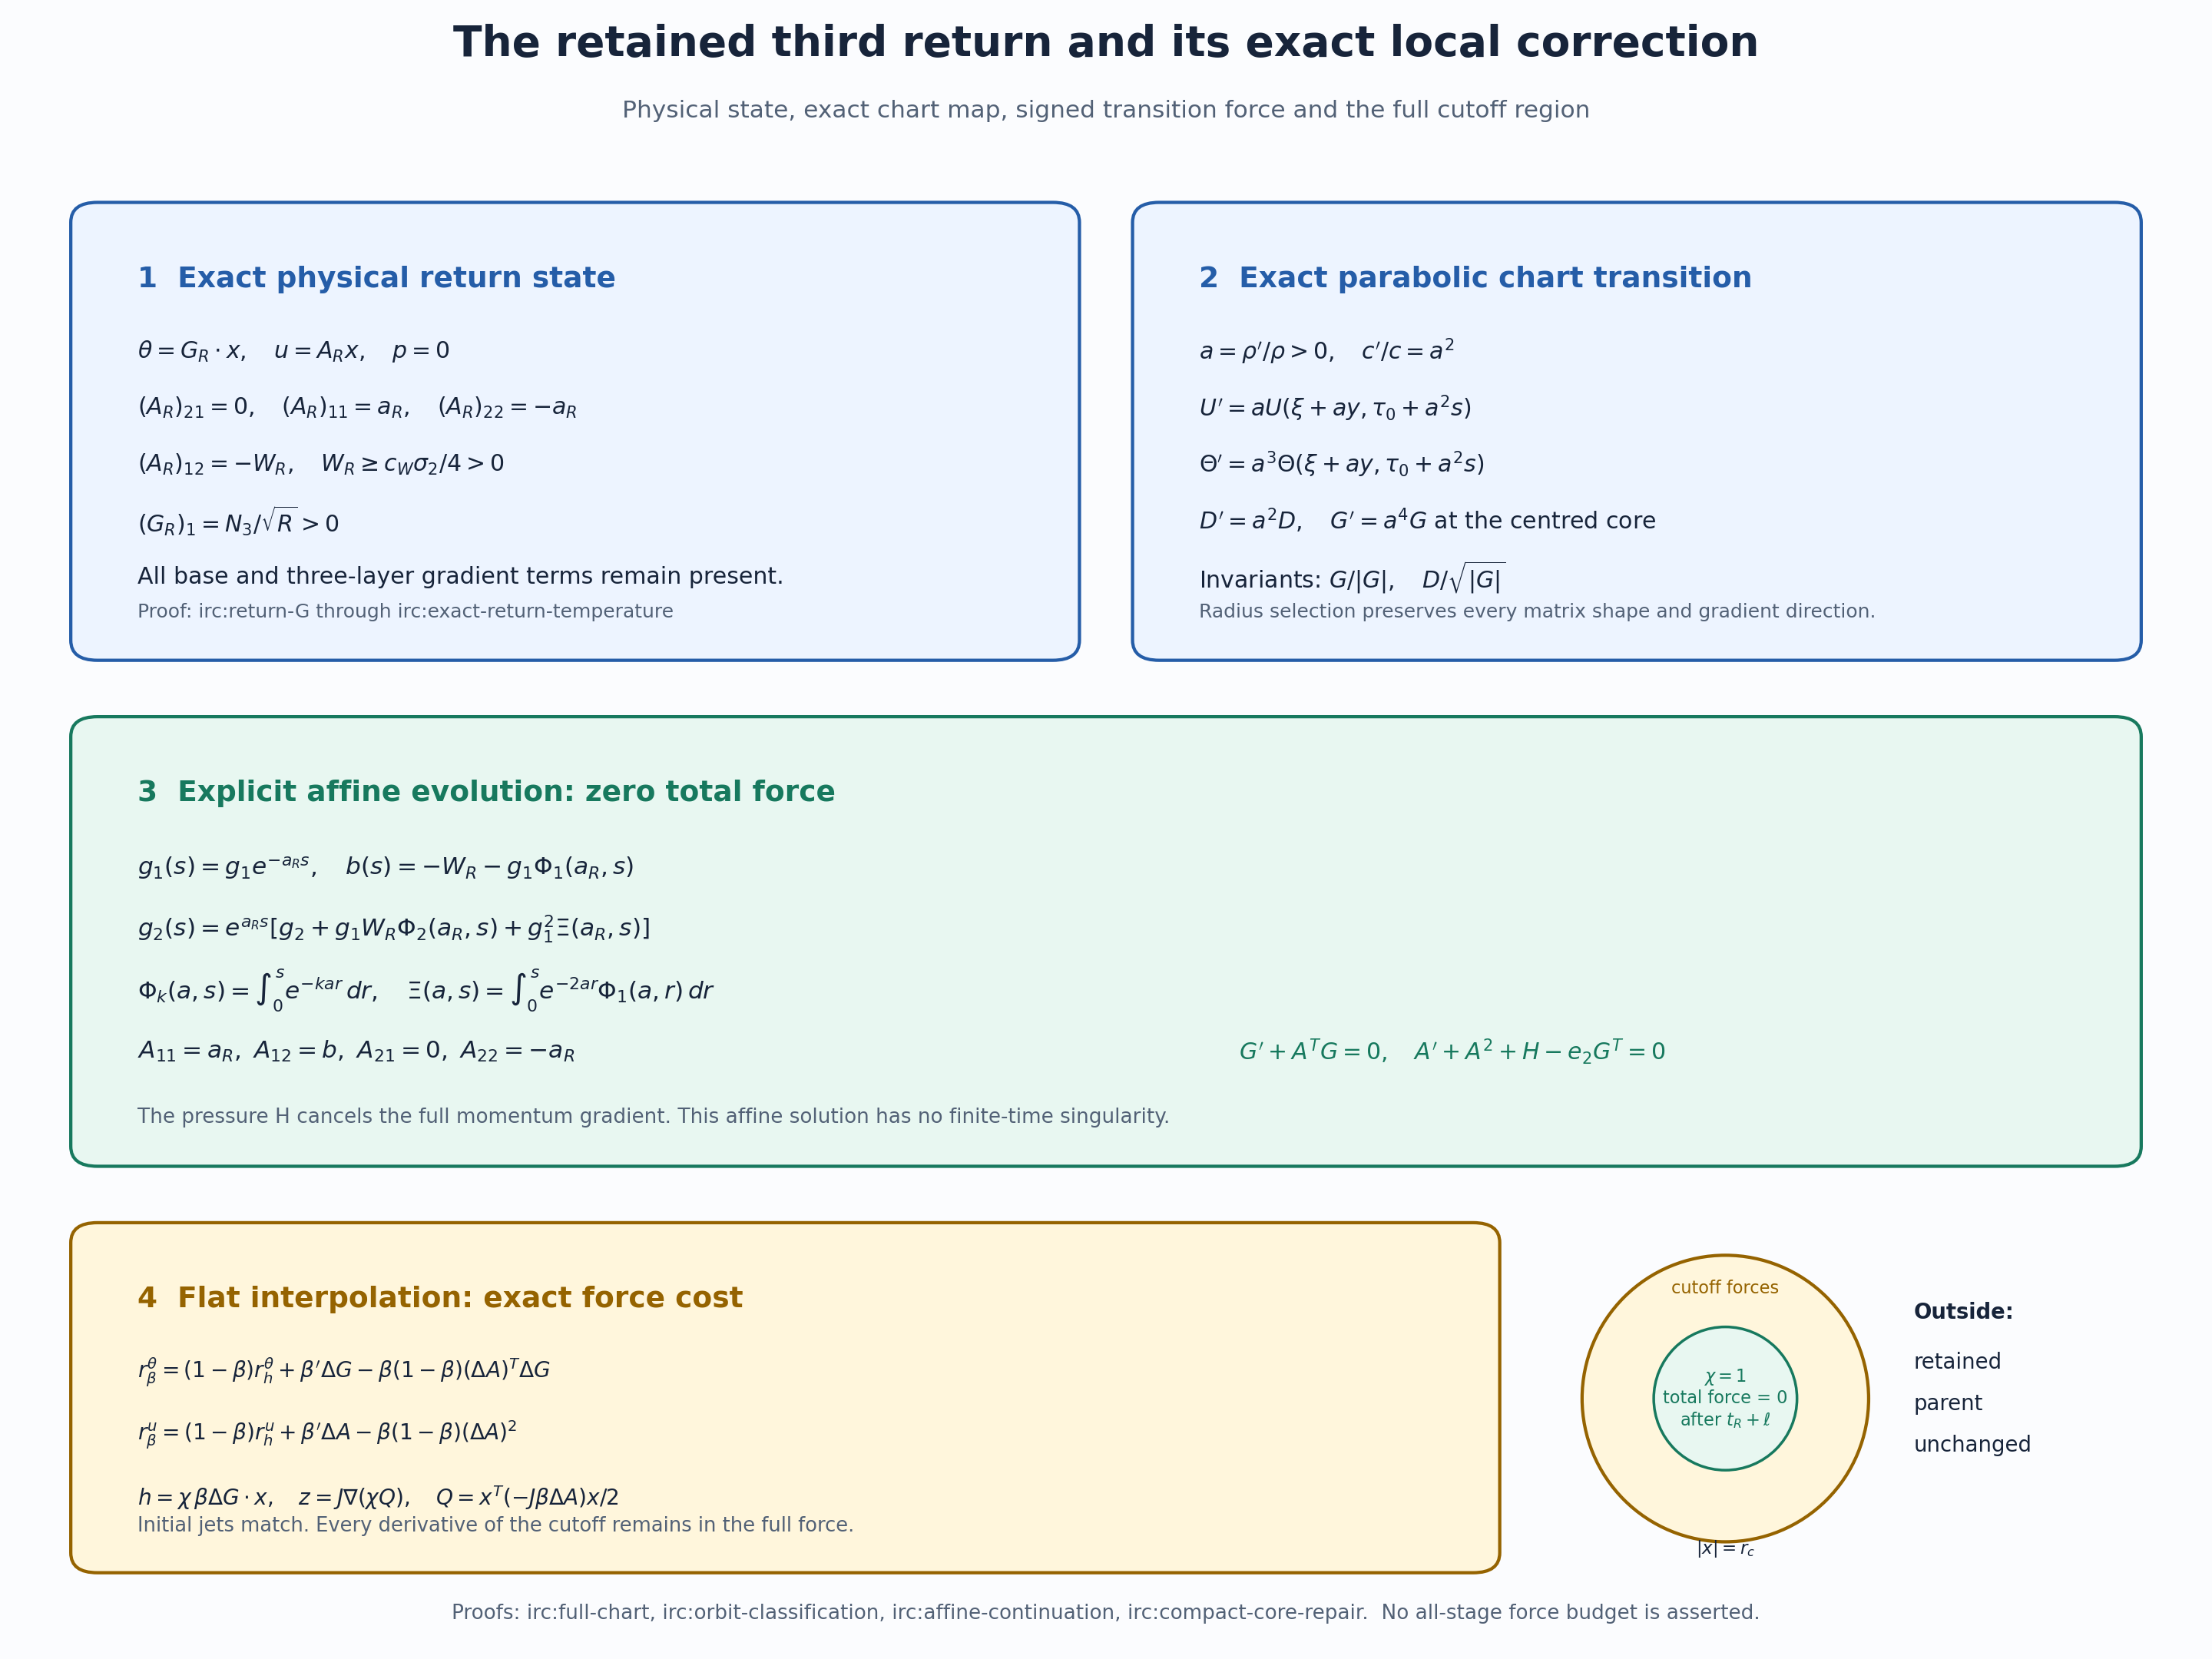
\includegraphics[width=0.97\linewidth]
 {infinite_modified/figures/return_correction.png}
 \caption{Exact third-return state and its compact local correction.
 The physical $G_1=N_3/\sqrt R$ and curl are positive, while every
 strain and vertical-gradient contribution remains present.
 Parabolic dilation preserves the displayed full state invariants.
 The explicit affine evolution cancels its total force.  A flat
 transition and a streamfunction cutoff preserve the old initial
 jets and localize the correction; their displayed signed terms
 are the force cost still to be controlled.}
 \label{irc:figure}
\end{figure}

\section{The complete compact-correction force and its annulus cost}
\label{ifs:section}

We now evaluate the operation of Proposition~\ref{irc:compact-core-repair}
on its whole support.  Let $I$ be its finite held interval, and choose
$0<r\leq r_c$, with the original $r_c$ and all its material and phase
restrictions retained.  On $B_r$ the actual old fields are
\[
 \theta_h(x,t)=G(t)\cdot x,\qquad u_h(x,t)=A(t)x,\qquad
 p_h(x,t)=\tfrac12 x^TH(t)x,\qquad \operatorname{tr}A=0.
\]
Here $A=A_h,G=G_h,H=H_h$ are the full earlier sums, not selected
components.  Fix a real $\psi\in C_c^\infty(B_1)$ with $\psi=1$ on
$B_{1/2}$, and use $\chi(x)=\psi(x/r)$ in
\eqref{irc:compact-correction}.  Write
$L=\beta\Delta A$, $g=\beta\Delta G$, $K=\beta\Delta H$, and
$B=-JL$, where $J=\left(\begin{smallmatrix}0&-1\\1&0\end{smallmatrix}\right)$.
Then $B$ and $K$ are symmetric and $\operatorname{tr}L=0$.
All coefficients remain time dependent.

\subsection{An exact force map on the complete support}

For an evaluation variable $y=x/r$, define
\begin{align}
 H_g(y)&=\psi(y)\,g\cdot y,&
 q_L(y)&=\tfrac12 y^T(-JL)y,\nonumber\\
 Z_L(y)&=\psi(y)Ly+q_L(y)J\nabla\psi(y),&
 P_K(y)&=\tfrac12\psi(y)y^TKy.
 \label{ifs:cutoff-maps}
\end{align}
These are explicit linear maps of $g,L,K$.  They do not replace the
physical fields: the exact comparison is
\begin{equation}\label{ifs:physical-fields}
 h(ry,t)=rH_{g(t)}(y),\qquad
 z(ry,t)=rZ_{L(t)}(y),\qquad
 \kappa(ry,t)=r^2P_{K(t)}(y).
\end{equation}
In particular $Z_L=J\nabla(\psi q_L)$ and
$\operatorname{div}_yZ_L=0$.
The complete \emph{increment} force is
\begin{align}
 e^\theta(ry,t)
 &=r\mathcal T(y,t)-\frac d r\Delta_y H_g(y),\nonumber\\
 \mathcal T
 &=H_{g'}+(Ay)\cdot\nabla H_g
       +Z_L\cdot G+Z_L\cdot\nabla H_g,
 \label{ifs:scalar-force}\\
 e^u(ry,t)
 &=r\mathcal V(y,t)-\frac d r\Delta_y Z_L(y),\nonumber\\
 \mathcal V
 &=Z_{L'}+AZ_L+(\nabla Z_L)Ay
       +(\nabla Z_L)Z_L+\nabla P_K-H_g e_2.
 \label{ifs:vector-force}
\end{align}
They vanish outside $B_r$.  On $B_{r/2}$ these formulas give exactly
the increment between the old affine residual and
\eqref{irc:transition-scalar}--\eqref{irc:transition-vector}.
The total force everywhere is $f_h+e$; in particular it remains $f_h$
outside $B_r$.  A force estimate for the increment cannot certify a
smaller total force outside that ball.

\begin{proof}
Substitute \eqref{ifs:physical-fields} in the physical subtraction
identities \eqref{ibc:scalar-residual}--\eqref{ibc:vector-residual}.
On the entire support, $u_h(ry)=rAy$,
$\nabla\theta_h=G$ and $\nabla u_h=A$.
One spatial derivative of $rH_g$ or $rZ_L$ removes the factor $r$;
two give $r^{-1}$, whereas $\nabla_x(r^2P_K)=r\nabla_yP_K$.
This gives each displayed term with its shown sign and factor.
All corrections and derivatives vanish near the boundary of $B_r$,
so extension by zero is smooth and the formulas hold globally.
\end{proof}

For example the scalar transport part, with $n=\nabla\psi$, is
\begin{align}
 \mathcal T
 ={}&\psi(g'+A^Tg+L^TG)\cdot y
       +\psi^2 g\cdot Ly+(g\cdot y)n\cdot Ay\nonumber\\
    &+q_L G\cdot Jn+\psi q_Lg\cdot Jn
       +\psi(g\cdot y)n\cdot Ly, \label{ifs:expanded-scalar}\\
 \Delta_yH_g
 ={}&(g\cdot y)\Delta\psi+2g\cdot n. \nonumber
\end{align}
The apparent term $q_L(g\cdot y)(Jn)\cdot n$ is exactly zero
because $J$ is skew symmetric; no other cutoff term was dropped.
For the vector part, put $Q=q_L$, $n=\nabla\psi$,
$S=\nabla^2\psi$ and $k=\tfrac12y^TKy$.  Its full expansion is
\begin{align}
 \mathcal V={}&\psi(L'+AL+LA+K-e_2g^T)y+\psi^2L^2y
       +q_{L'}Jn+QAJn\nonumber\\
 &+(Ly)(n\cdot Ay)+(Jn)((By)\cdot Ay)+QJS\,Ay\nonumber\\
 &+\psi QLJn+\psi(Ly)(n\cdot Ly)
       -Q(n\cdot Ly)Jn\nonumber\\
 &+\psi QJS\,Ly+Q^2JS\,Jn+kn,\label{ifs:expanded-vector}\\
 \Delta_y Z_L={}&(\Delta\psi)Ly+2L\nabla\psi
       +(\operatorname{tr}B)J\nabla\psi
       +2JS\,By+QJ\nabla\Delta\psi. \nonumber
\end{align}
Indeed $(By)\cdot Ly=0$ and $(By)\cdot Jn=-Ly\cdot n$,
as follows from $B=-JL$ and $J^TJ=1$.
These are exact identities retaining strain, pressure, buoyancy,
both quadratic interactions and all diffusion contributions.

\subsection{Every mixed jet and quantitative cutoff constants}

All norms below are Euclidean vector norms, their induced matrix
norms, and supremum norms on $B_1$.
For a multi-index $\gamma\in\mathbb N^2$ set
$\Psi_\gamma=\|\partial^\gamma\psi\|_\infty$ and
$\Phi_\gamma=\|\partial^\gamma\nabla\psi\|_\infty$.
Define the nonnegative constants
\begin{align}
 C^H_\gamma&=\Psi_\gamma+\sum_{j=1}^2
                        \gamma_j\Psi_{\gamma-e_j},\nonumber\\
 Q_\nu&=
 \begin{cases}
 1/2,&|\nu|=0,\\
 1,&1\leq|\nu|\leq2,\\
 0,&|\nu|>2,
 \end{cases}\nonumber\\
 C^Z_\gamma&=C^H_\gamma+
       \sum_{\nu\leq\gamma}\binom\gamma\nu Q_\nu\Phi_{\gamma-\nu},
 \qquad
 C^P_\gamma=\sum_{\nu\leq\gamma}
                   \binom\gamma\nu Q_\nu\Psi_{\gamma-\nu}.
 \label{ifs:constants}
\end{align}
A term with a negative multi-index is zero.
For any such array $C$, put
\[
 (\nabla C)_\gamma=\sum_{j=1}^2 C_{\gamma+e_j},\qquad
 (\Delta C)_\gamma=\sum_{j=1}^2 C_{\gamma+2e_j}.
\]
Let $p_\nu=1$ when $|\nu|\leq1$ and $p_\nu=0$ otherwise, and set
\begin{align}
 \mathfrak A_\gamma(C)
 &=\sum_{\nu\leq\gamma}\binom\gamma\nu
                         p_\nu(\nabla C)_{\gamma-\nu},\nonumber\\
 \mathfrak B_\gamma(C,D)
 &=\sum_{\nu\leq\gamma}\binom\gamma\nu
                         C_\nu(\nabla D)_{\gamma-\nu}.
 \label{ifs:product-constants}
\end{align}
These explicit constants depend only on the selected cutoff and jet,
not on $r,d$ or the parent coefficients.
The product rule and $|y|\leq1$ give
\begin{equation}\label{ifs:linear-map-bounds}
 \|\partial^\gamma H_g\|_\infty\leq C^H_\gamma|g|,
 \quad
 \|\partial^\gamma Z_L\|_\infty\leq C^Z_\gamma\|L\|,
 \quad
 \|\partial^\gamma P_K\|_\infty\leq C^P_\gamma\|K\|.
\end{equation}
To check every factor, derivatives of $g\cdot y$ have orders zero
and one, bounded by $|g|$.  Derivatives of either quadratic
$q_L$ or $y^TKy/2$ have bounds $Q_\nu\|L\|$ or
$Q_\nu\|K\|$, respectively.  Their higher derivatives vanish.
These facts prove \eqref{ifs:constants} term by term.

Write $\mathcal T_{\gamma,b}=\partial_y^\gamma\partial_t^b\mathcal T$
and $\mathcal V_{\gamma,b}=\partial_y^\gamma\partial_t^b\mathcal V$.
Their full signed formulas are
\begin{align}
 \mathcal T_{\gamma,b}
 ={}&\partial^\gamma H_{g^{(b+1)}}\nonumber\\
 &+\sum_{j=0}^b\binom bj\sum_{\nu\leq\gamma}\binom\gamma\nu
   \bigl(\partial^\nu(A^{(j)}y)\bigr)\cdot
          \nabla\partial^{\gamma-\nu}H_{g^{(b-j)}}\nonumber\\
 &+\sum_{j=0}^b\binom bj
       \partial^\gamma Z_{L^{(j)}}\cdot G^{(b-j)}\nonumber\\
 &+\sum_{j=0}^b\binom bj\sum_{\nu\leq\gamma}\binom\gamma\nu
       \partial^\nu Z_{L^{(j)}}\cdot
          \nabla\partial^{\gamma-\nu}H_{g^{(b-j)}},
 \label{ifs:scalar-jets}\\
 \mathcal V_{\gamma,b}
 ={}&\partial^\gamma Z_{L^{(b+1)}}
       +\sum_{j=0}^b\binom bj A^{(j)}
                            \partial^\gamma Z_{L^{(b-j)}}\nonumber\\
 &+\sum_{j=0}^b\binom bj\sum_{\nu\leq\gamma}\binom\gamma\nu
       (\nabla\partial^{\gamma-\nu} Z_{L^{(b-j)}})
                              \partial^\nu(A^{(j)}y)\nonumber\\
 &+\sum_{j=0}^b\binom bj\sum_{\nu\leq\gamma}\binom\gamma\nu
       (\nabla\partial^{\gamma-\nu} Z_{L^{(b-j)}})
                              \partial^\nu Z_{L^{(j)}}\nonumber\\
 &+\nabla\partial^\gamma P_{K^{(b)}}
       -\partial^\gamma H_{g^{(b)}}e_2.
 \label{ifs:vector-jets}
\end{align}
Thus, without interchanging cancellation and norms,
\begin{align}
 (\partial_x^\gamma\partial_t^b e^\theta)(ry,t)
 &=r^{1-|\gamma|}\mathcal T_{\gamma,b}
    -d r^{-1-|\gamma|}\Delta\partial^\gamma H_{g^{(b)}},
 \label{ifs:physical-scalar-jets}\\
 (\partial_x^\gamma\partial_t^b e^u)(ry,t)
 &=r^{1-|\gamma|}\mathcal V_{\gamma,b}
    -d r^{-1-|\gamma|}\Delta\partial^\gamma Z_{L^{(b)}}.
 \label{ifs:physical-vector-jets}
\end{align}
Time derivatives are physical time derivatives here; no clock
factor has been absorbed.

The following computable majorants preserve the complete coefficient
and derivative dependence:
\begin{align}
 T_{\gamma,b}={}&C^H_\gamma|g^{(b+1)}|
  +\sum_{j=0}^b\binom bj\bigl[
    \mathfrak A_\gamma(C^H)\|A^{(j)}\||g^{(b-j)}|\nonumber\\
 &\hspace{24mm}+C^Z_\gamma\|L^{(j)}\||G^{(b-j)}|
    +\mathfrak B_\gamma(C^Z,C^H)\|L^{(j)}\||g^{(b-j)}|\bigr],
 \label{ifs:scalar-majorant}\\
 V_{\gamma,b}={}&C^Z_\gamma\|L^{(b+1)}\|
  +\sum_{j=0}^b\binom bj\bigl[
    (C^Z_\gamma+\mathfrak A_\gamma(C^Z))
                         \|A^{(j)}\|\|L^{(b-j)}\|\nonumber\\
 &\hspace{24mm}+\mathfrak B_\gamma(C^Z,C^Z)
                         \|L^{(j)}\|\|L^{(b-j)}\|\bigr]\nonumber\\
 &+(\nabla C^P)_\gamma\|K^{(b)}\|+C^H_\gamma|g^{(b)}|.
 \label{ifs:vector-majorant}
\end{align}
Consequently the global increment jets satisfy
\begin{align}
 \|\partial_x^\gamma\partial_t^b e^\theta\|_\infty
 &\leq r^{1-|\gamma|}T_{\gamma,b}
       +d r^{-1-|\gamma|}(\Delta C^H)_\gamma |g^{(b)}|,
 \nonumber\\
 \|\partial_x^\gamma\partial_t^b e^u\|_\infty
 &\leq r^{1-|\gamma|}V_{\gamma,b}
       +d r^{-1-|\gamma|}(\Delta C^Z)_\gamma \|L^{(b)}\|.
 \label{ifs:force-majorants}
\end{align}
The Leibniz formulas above prove these inequalities, since a derivative
of $Ay$ has norm at most $\|A\|$ for orders zero or one, and zero
otherwise.  They are sufficient estimates only; the exact signed
expressions \eqref{ifs:physical-scalar-jets}--\eqref{ifs:physical-vector-jets}
are the force being estimated.

\subsection{A quantitative annulus obstruction and its exact defect}

\begin{lemma}\label{ifs:cutoff-diffusion-lower-bound}
The compact cutoff maps satisfy
\[
 \|\Delta H_g\|_\infty\geq2|g|,\qquad
 \|\Delta Z_L\|_\infty\geq2\|L\|.
\]
Their Laplacians are supported in the cutoff annulus
$B_1\setminus B_{1/2}$.
\end{lemma}

\begin{proof}
For a real $f\in C_c^\infty(B_1)$ put
$M=\|\Delta f\|_\infty$ and $w(y)=M(1-|y|^2)/4$.
Since $\Delta w=-M$ in two dimensions, $\Delta(f-w)\geq0$
and $\Delta(-f-w)\geq0$.  Both functions have zero boundary
values.  The maximum principle gives $|f|\leq w\leq M/4$.
Applying this to $H_g$, whose supremum is at least $|g|/2$
on the closed inner ball, proves its bound.
For $L\ne0$, choose a unit vector $v$ with $|Lv|=\|L\|$
and put $a=Lv/\|L\|$.  The scalar $f=a\cdot Z_L$ takes
the value $\|L\|/2$ at $v/2$, so
$\|\Delta Z_L\|_\infty\geq\|\Delta f\|_\infty\geq2\|L\|$.
The zero case is immediate.  On the inner ball the maps are
linear; outside $B_1$ they vanish.  Their Laplacians therefore
have the asserted annular support.
\end{proof}

At every physical time, the \emph{actual signed} force consequently
satisfies
\begin{align}
 \|e^\theta(t)\|_\infty
 &\geq\frac{2d}{r}|g(t)|-r\|\mathcal T(t)\|_\infty
  \geq\frac{2d}{r}|g(t)|-rT_{0,0}(t),\nonumber\\
 \|e^u(t)\|_\infty
 &\geq\frac{2d}{r}\|L(t)\|-r\|\mathcal V(t)\|_\infty
  \geq\frac{2d}{r}\|L(t)\|-rV_{0,0}(t).
 \label{ifs:force-lower-bounds}
\end{align}
This is the reverse triangle inequality, not a claim that diffusion
alone is the force.  In particular a fixed nonzero coefficient
correction at a fixed time, with fixed finite coefficient derivatives,
cannot have an increment force tending to zero merely by letting
$r\downarrow0$.  Its force instead diverges at that time.
The conclusion applies to this precisely specified compact operation.
It does not exclude trajectories whose coefficients or time scales
vary with $r$, or corrections that achieve additional cancellations.

The exact objects which describe the missing cancellation are
\begin{equation}\label{ifs:defect-maps}
 \mathcal D^\theta_r=\frac{r^2}{d}\mathcal T-\Delta H_g,\qquad
 \mathcal D^u_r=\frac{r^2}{d}\mathcal V-\Delta Z_L.
\end{equation}
They are smooth, supported in $B_1$, and satisfy the full morphism
\[
 e^\theta(ry,t)=\frac d r\mathcal D^\theta_r(y,t),\qquad
 e^u(ry,t)=\frac d r\mathcal D^u_r(y,t).
\]
The corresponding mixed-jet map has the exact factor
$d r^{-1-|\gamma|}$ and no time factor.  Thus a bound
$\|\partial_x^\gamma\partial_t^b e\|_\infty\leq\varepsilon$
is \emph{equivalent} to
$\|\partial_y^\gamma\partial_t^b\mathcal D_r\|_\infty
\leq(\varepsilon/d)r^{1+|\gamma|}$, with scalar and vector
components kept separately.
This defines the precise cancellation space for this operation
and its map to the physical all-jet force budget.

The next operation must control these complete defects, retain the
outer parent force, and still realize a subsequent growing return.
The fixed-coefficient localized affine repair does not accomplish
that operation.  Its finite full-support force, every mixed derivative,
and its exact small-force requirement have now been calculated;
the next based return and the infinite smooth-force construction
remain unfinished.  The identities are checked by
\path{full_support_force_check.py} in \path{infinite_modified/checks}.

\begin{figure}[htbp]
 \centering
 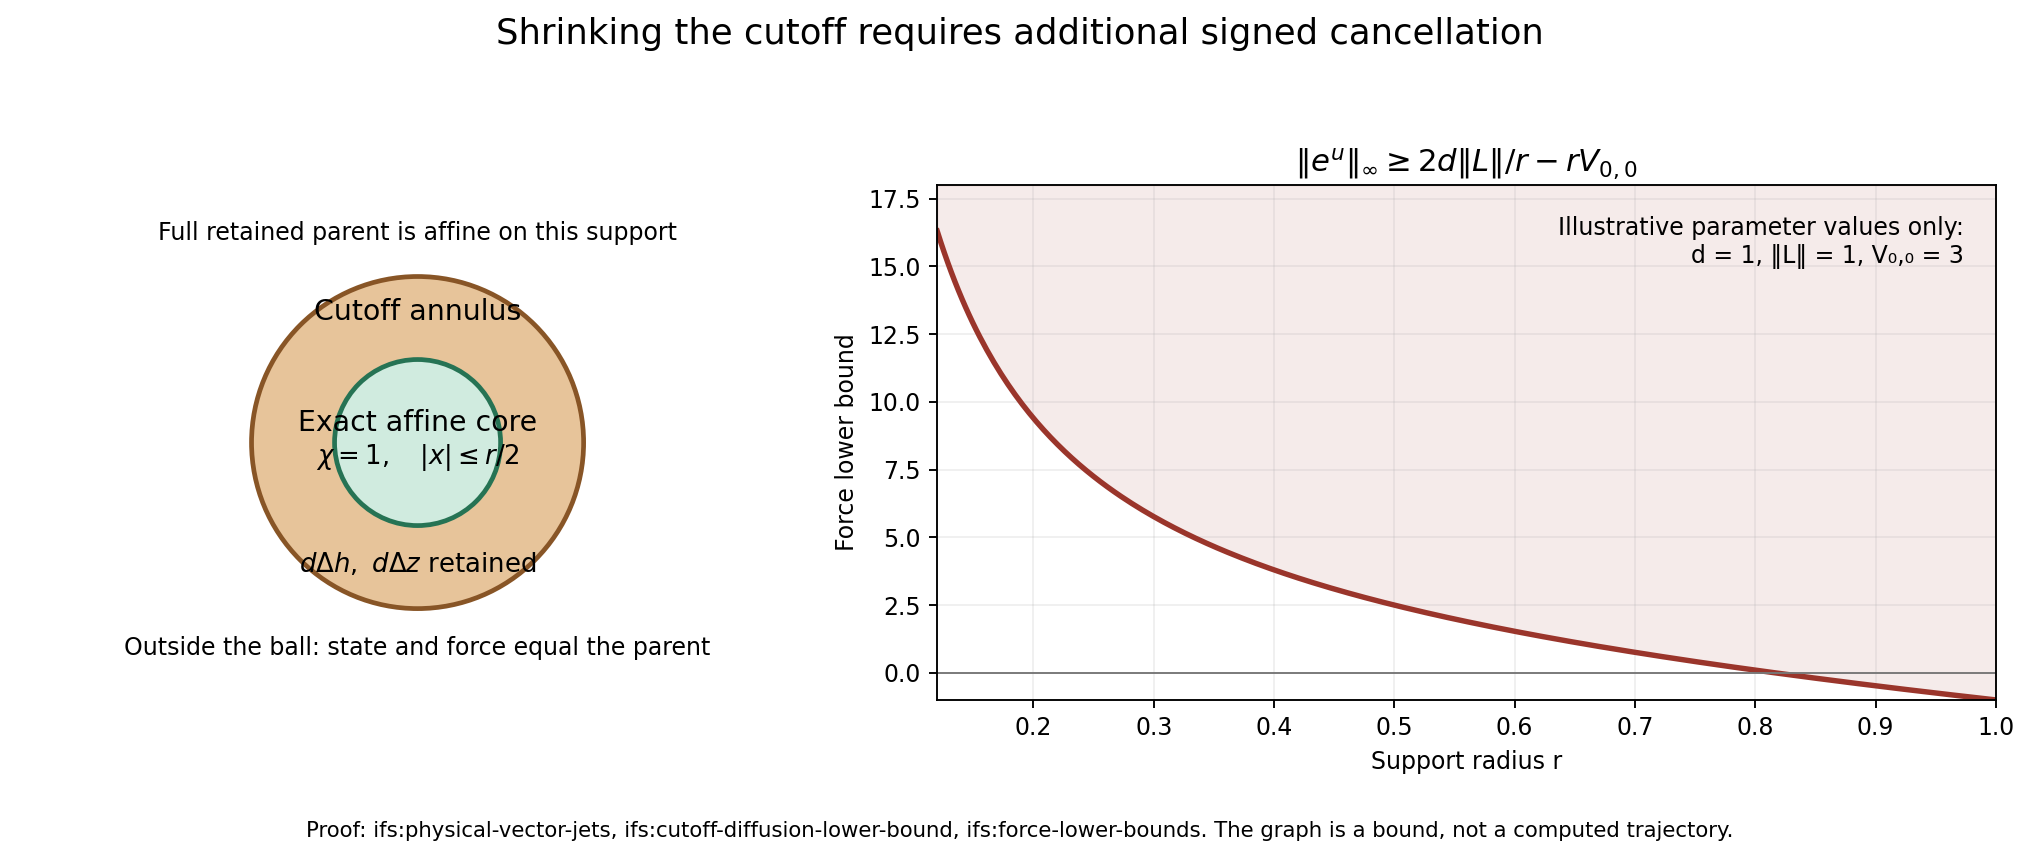
\includegraphics[width=0.97\linewidth]
 {infinite_modified/figures/full_support_force.png}
 \caption{The actual affine parent region permits evaluation of the entire
 compact correction.  Both cutoff Laplacians live in the annulus.
 The graph shows only the proved lower-bound expression at the displayed
 illustrative parameter values, not a sampled solution.  All physical
 diffusion and radius factors remain in the formulas.  The cutoff
 comparison and its proof are \eqref{ifs:physical-fields},
 Lemma~\ref{ifs:cutoff-diffusion-lower-bound} and
 \eqref{ifs:force-lower-bounds}; the source profile is retained from
 Alp\"oge--Buckmaster, Sections 3.3 and 3.7.10.}
 \label{ifs:figure}
\end{figure}

\section{The exact force needed to reach a compact based state}
\label{ifr:section}

The annulus defect has a further finite-interval consequence for the
actual signed force.  Retain the entire smooth parent
$(\theta_P,u_P,p_P)$ on $[a,b]$, and let a compact smooth increment
$(h,z,\kappa)$ have $\operatorname{div}z=0$ and $h(a)=z(a)=0$.
The support of the increment is contained in one fixed compact set on
this finite interval.  Write $e^\theta,e^u$ for its complete physical
residual \eqref{ibc:scalar-residual}--\eqref{ibc:vector-residual}.
No assumption that the parent's own force vanishes is made.

For every retained weight $\lambda>0$, define the original-coordinate
quantities
\begin{align}
 E_\lambda(t)^2&=\|z(t)\|_2^2+\lambda\|h(t)\|_2^2,\nonumber\\
 F_\lambda(t)^2&=\|e^u(t)\|_2^2+\lambda\|e^\theta(t)\|_2^2,\nonumber\\
 C_\lambda(t)&=\|\nabla u_P(t)\|_\infty+
             \frac{1+\lambda\|\nabla\theta_P(t)\|_\infty}
                  {2\sqrt\lambda}.
 \label{ifr:weighted-data}
\end{align}
The parent norms may be restricted to the common compact support
neighbourhood; using the full spatial norms also gives the displayed
bounds.  The diffusion coefficient $d>0$ is unchanged.
The exact energy identity is
\begin{align}
 \frac12(E_\lambda^2)'&
   +d\bigl(\|\nabla z\|_2^2+\lambda\|\nabla h\|_2^2\bigr)\nonumber\\
 &= -\int z^T(\nabla u_P)z
    -\lambda\int h\,z\cdot\nabla\theta_P
    +\int h z_2
    +\int z\cdot e^u+\lambda\int h e^\theta .
 \label{ifr:energy-identity}
\end{align}
All integrals use the original Lebesgue measure on $\mathbb R^2$.

\begin{proof}
Multiply the scalar increment equation by $\lambda h$ and the vector
increment equation by $z$, then integrate and add.
Both $u_P$ and $z$ are divergence free.  Therefore
$\int h\,u_P\cdot\nabla h$, $\int h\,z\cdot\nabla h$,
$\int z\cdot(u_P\cdot\nabla)z$, and
$\int z\cdot(z\cdot\nabla)z$ vanish by integration by parts.
The pressure integral $\int z\cdot\nabla\kappa$ also vanishes.
The term $(z\cdot\nabla)u_P$ gives the first right-hand integral.
The scalar parent-gradient term gives the second, and the original
buoyancy $-he_2$ on the residual's left side gives the third with a
positive sign.  Each retained $-d\Delta$ term gives the corresponding
positive gradient norm.  Compact support removes the spatial boundary
terms.  This proves the full identity, including all signs and $\lambda$.
\end{proof}

The parent-gradient and buoyancy terms obey
\[
 \left|-\lambda\int h\,z\cdot\nabla\theta_P+\int h z_2\right|
 \leq\frac{1+\lambda\|\nabla\theta_P\|_\infty}
             {2\sqrt\lambda}E_\lambda^2.
\]
Indeed their sum is bounded by
$(1+\lambda\|\nabla\theta_P\|_\infty)\|h\|_2\|z\|_2$,
and $2\sqrt\lambda\|h\|_2\|z\|_2\leq E_\lambda^2$.
The strain term is at most
$\|\nabla u_P\|_\infty E_\lambda^2$, and the signed forcing
pairing is at most $E_\lambda F_\lambda$.
Dropping only the displayed nonnegative diffusion integral in this
inequality gives the exact finite-interval estimate
\begin{equation}\label{ifr:reachability-bound}
 E_\lambda(t)\leq
 \int_a^t
   \exp\!\left(\int_s^t C_\lambda(\tau)\,d\tau\right)
       F_\lambda(s)\,ds .
\end{equation}
For a proof valid at zeros of $E_\lambda$, put
$E_{\lambda,\varepsilon}=(E_\lambda^2+\varepsilon^2)^{1/2}$.
The energy identity implies
$E_{\lambda,\varepsilon}'\leq
C_\lambda E_{\lambda,\varepsilon}+F_\lambda$.
Multiply by $\exp(-\int_a^t C_\lambda)$, integrate, and let
$\varepsilon\downarrow0$.  Its initial value is $\varepsilon$;
the stated formula follows.

In particular, the force-to-state map has zero kernel at this based
initial state: $e^\theta=e^u=0$ throughout the interval implies
$h=z=0$ throughout the interval.  It also gives the nonzero target cost
\begin{equation}\label{ifr:force-cost}
 \int_a^t F_\lambda(s)\,ds
 \geq
 \exp\!\left(-\int_a^t C_\lambda(\tau)\,d\tau\right)E_\lambda(t).
\end{equation}
This uses $C_\lambda\geq0$ in \eqref{ifr:reachability-bound}.
It relates the actual signed residual to a reached state, not to the
unsigned termwise majorants rejected earlier.

For the compact affine correction \eqref{ifs:physical-fields},
the target has a further exact lower bound:
\begin{equation}\label{ifr:affine-target-cost}
 E_\lambda(t)\geq
 \frac{\sqrt\pi\,r^2}{8}
 \left(\|L(t)\|_{\mathrm F}^2+\lambda|g(t)|^2\right)^{1/2}.
\end{equation}
To prove it, integrate only over $B_{r/2}$, where
$z=Lx$ and $h=g\cdot x$.  The original coordinate integrals are
\[
 \int_{B_{r/2}}x_i x_j\,dx
    =\delta_{ij}\frac{\pi r^4}{64}.
\]
Thus $\int|Lx|^2=(\pi r^4/64)\operatorname{tr}(L^TL)$
and $\int|g\cdot x|^2=(\pi r^4/64)|g|^2$ on that ball,
which proves the formula with the full Frobenius norm.
Combining \eqref{ifr:force-cost} and
\eqref{ifr:affine-target-cost} gives a quantitative necessary
physical $L^1_tL^2_x$ force budget for the complete compact operation.
Every radius, weight, parent gradient and exponential remains explicit.

This calculation supplies the next test for a proposed annulus
correction: it must satisfy the signed defect requirement
\eqref{ifs:defect-maps} and the complete-state cost
\eqref{ifr:force-cost}.  The estimate neither bounds the successive
parent gradients uniformly nor constructs the next growing return.
Those receiving calculations remain active.  The zero-kernel result
shows why simply replacing the whole increment by a zero-force
evolution from its unchanged initial jets would erase the increment
itself.  A successful construction must retain and estimate the actual
control that reaches its new state.

\appendix
\clearpage
\section{Full source controls and aggregate background identities}
\paragraph{Source and scope.}
The source is Levent Alp\"oge and Tristan Buckmaster, \emph{Blowup for the Boussinesq equations with smooth forcing}, the supplied 76-page released PDF. Page numbers below are the printed PDF page numbers. The companion source receipt identifies the exact local PDF by SHA-256. The equations and proofs here reconstruct the finite-dimensional system in Section 3, especially pp.~8--10 and 26--33, and its exact affine realization in Section 4, pp.~37--39. The source's local comparison bounds are identified as source results where mentioned; the new claims proved below are the coordinate, operator, feedback, and aggregate-background identities. No infinite retained-viscosity construction is asserted.

\paragraph{Original data and the distinct parameters.}
Keep the original data of source (1.4), p.~2:
\[
 A_0\ge1,\qquad \lambda_0=\left\lceil\frac{\sqrt{A_0}}2\right\rceil,
 \qquad \theta_{\rm in}(x)=-\frac{A_0}{\lambda_0}\sin(\lambda_0x_2)\chi_0(x),
 \qquad u_{\rm in}=0.
\]
Here $\chi_0\in C_c^\infty(B_{R_0})$ is radial, $R_0>2$, $0\le\chi_0\le1$, and $\chi_0=1$ on $B_2$. Write
\[
 \mu=\lambda_0,\qquad \nu_{\AB}=\sqrt{A_0},\qquad X=\mu x,\quad T=\nu_{\AB}t.
\]
The symbol $\nu_{\AB}$ is precisely the time-scaling parameter called $\nu$ in source Lemma 1.2, pp.~6--7. It is not physical viscosity. Physical momentum viscosity is $\epsv\ge0$ and thermal diffusivity is $\kapth\ge0$. The source uses $\mu$ again locally for its shooting amplitude; we display that independent parameter as $\mu_{\rm p}$, and never identify it with $\mu=\lambda_0$.

Use a hat for a source Section 3 quantity, which is expressed there in $(X,T)$. The exact dictionary, keeping both presentations, is
\begin{align}
 \theta(x,t)&=\frac{\nu_{\AB}^2}{\mu}\widehat\theta(X,T),&
 u(x,t)&=\frac{\nu_{\AB}}\mu\widehat u(X,T),&
 p(x,t)&=\frac{\nu_{\AB}^2}{\mu^2}\widehat p(X,T),\label{pc:eq:scaling}\\
 \omega(x,t)&=\nu_{\AB}\widehat\omega(X,T),&
 \psi(x,t)&=\frac{\nu_{\AB}}{\mu^2}\widehat\psi(X,T),\nonumber\\
 f_\theta(x,t)&=\frac{\nu_{\AB}^3}{\mu}\widehat f_\theta(X,T),&
 f_u(x,t)&=\frac{\nu_{\AB}^2}{\mu}\widehat f_u(X,T).\nonumber
\end{align}
The transformed diffusivities are
\begin{equation}\label{pc:eq:scaled-diffusion}
 \widehat\kapth=\kapth\frac{\mu^2}{\nu_{\AB}},\qquad
 \widehat\epsv=\epsv\frac{\mu^2}{\nu_{\AB}}.
\end{equation}
These statements follow directly from $\partial_t=\nu_{\AB}\partial_T$, $\nabla_x=\mu\nabla_X$, and $\Delta_x=\mu^2\Delta_X$: both scalar transport terms have factor $\nu_{\AB}^3/\mu$, both momentum transport terms and gravity have factor $\nu_{\AB}^2/\mu$, and the respective Laplacian terms have factors $\kapth\nu_{\AB}^2\mu$ and $\epsv\nu_{\AB}\mu$. The divergence scales by $\nu_{\AB}$, curl by $\nu_{\AB}$, and $J\nabla_x\psi=(\nu_{\AB}/\mu)J\nabla_X\widehat\psi$. Thus the laboratory gravity vector $e_2=(0,1)$ is unchanged. The inverse transformations divide by the displayed nonzero factors and evaluate at $(x,t)=(X/\mu,T/\nu_{\AB})$, so these are bijections of the corresponding smooth fields, with support radii divided by $\mu$ and time intervals divided by $\nu_{\AB}$.

\paragraph{Layer dictionary.}
For $j\ge1$ retain the original source $\widehat\lambda_j$, and define its actual spatial frequency $\lambda_j=\mu\widehat\lambda_j$. The remaining dictionary is
\begin{align}
 M_j(t)&=\widehat M_j(\nu_{\AB}t),&\zeta_j(t)&=\widehat\zeta_j(\nu_{\AB}t),&p_j&=\widehat p_j,\\
 \Theta_j(t)&=\frac{\nu_{\AB}^2}{\mu}\widehat\Theta_j(\nu_{\AB}t),&
 \Omega_j(t)&=\nu_{\AB}\widehat\Omega_j(\nu_{\AB}t),&
 \alpha(t)&=\widehat\alpha(\nu_{\AB}t),\nonumber\\
 A_j(t)&=\nu_{\AB}^2\widehat A_j(\nu_{\AB}t),&
 \sigma_j&=\nu_{\AB}\widehat\sigma_j,&
 \Gamma_j&=\nu_{\AB}\widehat\Gamma_j,\nonumber\\
 D_{<j}(t)&=\nu_{\AB}\widehat D_{<j}(\nu_{\AB}t),&
 G_{<j}(t)&=\nu_{\AB}^2\widehat G_{<j}(\nu_{\AB}t),&
 \ell_j&=\widehat\ell_j/\mu.\nonumber
\end{align}
In particular $\sigma_0=\nu_{\AB}$, $A_0=\nu_{\AB}^2$, and the original $\lambda_0=\mu$ has not been reset. All unadorned derivatives below are in original physical time $t$.

\paragraph{The exact coupled variables.}
Let
\[
 J=\begin{pmatrix}0&-1\\1&0\end{pmatrix},\quad
 e(\phi)=(\sin\phi,\cos\phi),\quad e_0=R_\alpha e_2=e(-\alpha),\quad w_0=1.
\]
For $j\ge1$ set $r_j=|\zeta_j|$, $e_j=\zeta_j/r_j=e(\phi_j)$, $P_j=-\Theta_j$, $A_j=\lambda_jr_jP_j$, and $B_j=\lambda_j\Theta_j\zeta_j=-A_je_j$. The positive-amplitude variables are used only on intervals where their positivity has been established. Put $B_0=-A_0e_0$, and
\begin{equation}\label{pc:eq:coupled}
 \begin{aligned}
 G_{<j}&=B_0+\sum_{1\le i<j}w_iB_i,
 &D_{<j}&=\dot\alpha J+\sum_{1\le i<j}w_iS_i,
 &S_i&=\Omega_iJe_i\otimes e_i,\\
 \dot M_j&=D_{<j}M_j,
 &M_j(t_j^{\rm in})&=I,
 &\zeta_j&=M_j^{-T}p_j,\\
 \dot\Theta_j&=a_j\Omega_j,
 &a_j&=-\frac{J\zeta_j\cdot G_{<j}}{\lambda_jr_j^2},
 &\dot\Omega_j&=b_j\Theta_j,\quad b_j=\lambda_j\zeta_{j,1}.
 \end{aligned}
\end{equation}
These are source (3.2)--(3.3), p.~8, in original units. To check their scaling, $a_j=(\nu_{\AB}^2/\mu)\widehat a_j$ and $b_j=\mu\widehat b_j$; consequently both amplitude equations have their correct factors $\nu_{\AB}^3/\mu$ and $\nu_{\AB}^2$. Since $\tr J=\tr(Je_i\otimes e_i)=0$, Jacobi's determinant formula gives $\det M_j=1$ throughout every finite existence interval.

\paragraph{Derivation of the wave equations.}
Let $F$ be the exact odd smooth periodic profile of source (4.1), and let $\mathcal P$ be its even mean-zero primitive. Put $s=\lambda_j\zeta_j\cdot x$ and
\[
 \vartheta_j=\Theta_jF(s),\quad
 \psi_j=\frac{\Omega_j}{\lambda_j^2r_j^2}\mathcal P(s),\quad
 v_j=\frac{\Omega_j}{\lambda_jr_j^2}J\zeta_j F(s),\quad
 \varpi_j=\Omega_jF'(s).
\]
Differentiating $M_j^{-T}p_j$ gives $\dot\zeta_j=-D_{<j}^T\zeta_j$, hence $(\partial_t+D_{<j}x\cdot\nabla)s=0$. Moreover $J\zeta_j\cdot\zeta_j=0$, so $v_j\cdot\nabla\vartheta_j=v_j\cdot\nabla\varpi_j=0$. On an affine earlier state $G_{<j}\cdot x,D_{<j}x$, the added scalar residual is $(\dot\Theta_j+\Omega_jJ\zeta_j\cdot G_{<j}/(\lambda_jr_j^2))F$, and the added vorticity residual is $(\dot\Omega_j-\lambda_j\zeta_{j,1}\Theta_j)F'$. This proves the exact map from \eqref{pc:eq:coupled} to the unactivated local wave equations, including the fixed sign and gravity component.

\paragraph{The control maps and every stage.}
Source (3.4), p.~9, defines
\begin{equation}\label{pc:eq:feedback}
 F_j^{\rm ctl}=-\frac{\sum_{1\le i<j}w_i\Omega_i e_{i,1}(Je_i\cdot\zeta_j)}{\zeta_{j,2}},\qquad F_0^{\rm ctl}=0.
\end{equation}
The superscript distinguishes the paper's feedback $F_j$ from its periodic profile $F$. Transposing $D_{<j}$ in \eqref{pc:eq:coupled} and taking component one gives
\[
 \dot\zeta_{j,1}=(F_j^{\rm ctl}-\dot\alpha)\zeta_{j,2}.
\]
Thus $\dot\alpha=F_j^{\rm ctl}-\dot Z/\zeta_{j,2}$ implies $\zeta_{j,1}(t)=Z(t)$ whenever equality holds initially and the second component is nonzero. This proves the feedback map; the second component is not replaced by a constant.

Here is the complete source schedule (3.7)--(3.12), pp.~9--10, preserving its units. Fix $\beta=1/8$, $Q_*\ge200$, $Q_j=Q_*+j$, and
\begin{align}
 \widehat\lambda_1&\gg1,\qquad\widehat\lambda_j=\widehat\lambda_{j-1}^{Q_j}\quad(j\ge2),\label{pc:eq:schedule}\\
 \widehat\ell_1&=s_0/C_\ell,\quad C_\ell\ge4,\qquad\widehat\ell_j=\widehat\lambda_{j-1}^{-3}\quad(j\ge2),\nonumber\\
 \widehat\Pi_1&=(\log\widehat\lambda_1)^{10},\qquad
 \widehat\Pi_j=\widehat\lambda_{j-1}^{4}(\log\widehat\lambda_j)^{10}\quad(j\ge2),\nonumber\\
 k_j&=\max\{k\in\mathbb N_0:120k\le Q_j,\ K(k)\le\log\widehat\lambda_j\},\nonumber\\
 J_j&=2k_j+8,\qquad L_j=(k_j+5+\beta)\log\widehat\lambda_j.\nonumber
\end{align}
The prescribed seed is $\Theta_j^{\rm seed}=-(\nu_{\AB}^2/\mu)\widehat\lambda_j^{-k_j-6}$, and its gain target is
\[
 P_j(t_j^a)=\frac{\nu_{\AB}^2}{\mu}\widehat\lambda_j^{-7/8},
 \qquad \frac{P_j(t_j^a)}{|\Theta_j^{\rm seed}|}=e^{L_j}.
\]
In particular the physical frequency recursion is $\lambda_j=\mu(\lambda_{j-1}/\mu)^{Q_j}$, not $\lambda_{j-1}^{Q_j}$.
Let $\eta$ be smooth nondecreasing, zero on $(-\infty,0]$ and one on $[1,\infty)$; let $\eta_2\in C_c^\infty((0,1))$, $\eta_2\ge0$, $\int_0^1\eta_2=1$, and $H_2=\|\eta_2\|_\infty$. The fixed design is
\[
 c_p=3,\quad\bar v=2,\quad\Lambda_1\ge2c_pH_2,\quad
 0<s_*\le1/8,\quad c_p\Lambda_1H_2\sin s_*\le1/4.
\]
Set $t_1^{\rm in}=1/\nu_{\AB}$, $s_1=s_*$, $\Gamma_1=\nu_{\AB}\sin s_*$, and for $j\ge2$
\[
 t_j^{\rm in}=t_{j-1}^b,\quad s_j=L_j\frac{\sigma_{j-2}}{\sigma_{j-1}},\quad
 \Gamma_j=\sigma_{j-1}\sin s_j,\quad\Lambda_j=L_j.
\]
At activation $p_j=e(s_j)$, $\Theta_j=\Theta_j^{\rm seed}$, $\Omega_j=\sqrt{b_j/a_j}\Theta_j$, where source Theorem 3.2 proves $a_j,b_j>0$ on the constructed growth interval. The activation multiplier is $w_j(t)=\eta(\Gamma_j(t-t_j^{\rm in}))$.
\begin{enumerate}
\item Growth: $\dot\alpha=F_{j-1}^{\rm ctl}$ until the first amplitude threshold $t_j^a$ displayed above.
\item Transition: $t_j^1=t_j^a+\Gamma_j^{-1}$, $\eta_b=\eta(\Gamma_j(t-t_j^a))$, and $\dot\alpha=(1-\eta_b)F_{j-1}^{\rm ctl}+\eta_b F_j^{\rm ctl}$.
\item Steering: write $z_1=\zeta_{j,1}(t_j^1)$ and $\chi_1=r_j(t_j^1)$. For $0\le h\le h_j^{\max}=c_p\Lambda_j\sin s_j$ define
\[
 Z_j(t)=z_1[1-\eta(\Gamma_j(t-t_j^1))]
 -h\chi_1\eta_2\bigl(\Lambda_j\Gamma_j(t-t_j^1-\Gamma_j^{-1})\bigr),
\]
and $\dot\alpha=F_j^{\rm ctl}-\dot Z_j/\zeta_{j,2}$. The fixed endpoint is $t_j^b=t_j^1+\Gamma_j^{-1}(1+\Lambda_j^{-1})$. Select the least $h$ in the compact zero set $\Omega_j(t_j^b;h)=0$ proved nonempty in the source. No uniqueness is asserted for $j\ge2$.
\item Holding: use $\dot\alpha=F_j^{\rm ctl}$ through $t_{j+1}^a$, concurrently with next-layer growth; evaluate $\sigma_j^2=|G_{<j+1}(t_j^b)|$ only after selecting the stage. Since $\zeta_{j,1}=\Omega_j=0$, both $\dot\Omega_j=0$ and $\dot\Theta_j=0$. This proves stationarity of this amplitude pair, while the older state and $M_j$ may continue to evolve.
\end{enumerate}
All these control maps are in physical time; $F_j^{\rm ctl}=\nu_{\AB}\widehat F_j^{\rm ctl}$, and $Z_j$ is dimensionless. The source's smooth time joins follow from flatness of $\eta$, interior support of $\eta_2$, and uniqueness for the stationary endpoint pair.

\paragraph{Exact aggregate parent evolution.}
The following identities explicitly give the background feedback rather than prescribing $D,G$ independently.
\begin{proposition}\label{pc:prop:aggregate}
For every finite activated system \eqref{pc:eq:coupled}, put $G=G_{<q}$, $D=D_{<q}$, and $C=D_{21}-D_{12}=2\dot\alpha+\sum_{i<q}w_i\Omega_i$. Then
\begin{align}
 \dot G+D^TG&=\sum_{1\le i<q}\dot w_i B_i,\label{pc:eq:Gdot}\\
 \dot C-G_1&=2\ddot\alpha-A_0\sin\alpha+\sum_{1\le i<q}\dot w_i\Omega_i,\label{pc:eq:Cdot}\\
 \dot D&=\ddot\alpha J+\sum_{1\le i<q}(\dot w_i\Omega_i+w_i b_i\Theta_i)Je_i\otimes e_i\nonumber\\
 &\hspace{10mm}+\sum_{1\le i<q}w_i\Omega_i(\dot\alpha+\Sigma_i)
 (Je_i\otimes Je_i-e_i\otimes e_i),\label{pc:eq:Ddot}\\
 \Sigma_i&=\sum_{1\le k<i}w_k\Omega_k\sin^2(\phi_i-\phi_k).\nonumber
\end{align}
\end{proposition}
\begin{proof}
Differentiate $B_i=\lambda_i\Theta_i\zeta_i$ and use \eqref{pc:eq:coupled}:
\[
 \dot B_i+D_{<i}^TB_i
 =-\Omega_i e_i(Je_i\cdot G_{<i})=-S_i^TG_{<i}.
\]
Also $\dot B_0+ (\dot\alpha J)^TB_0=0$. Expand $\dot G+D^TG$, insert these equalities, and keep all cross terms. Its nonactivation terms are
\[
 \sum_i w_i S_i^TB_0-
 \sum_iw_iS_i^T\Bigl(B_0+\sum_{k<i}w_kB_k\Bigr)
 +\sum_iw_i\sum_{k\ge i}w_kS_k^TB_i.
\]
The $B_0$ terms cancel. The terms with $k>i$ in the last sum cancel the preceding double sum after exchanging its indices. Its diagonal terms are $w_i^2S_i^TB_i=0$, because $Je_i\cdot e_i=0$. This proves \eqref{pc:eq:Gdot} with every activation derivative retained. Next $\dot C=2\ddot\alpha+\sum_i\dot w_i\Omega_i+\sum_iw_i\lambda_i\zeta_{i,1}\Theta_i$, while $G_1=B_{0,1}+\sum_iw_i\lambda_i\Theta_i\zeta_{i,1}$ and $B_{0,1}=A_0\sin\alpha$. Subtraction proves \eqref{pc:eq:Cdot}. Finally direct projection of $\dot\zeta_i=-D_{<i}^T\zeta_i$ onto $e_i$ and $Je_i$ gives $\dot e_i=(\dot\alpha+\Sigma_i)Je_i$. Differentiate $S_i=\Omega_iJe_i\otimes e_i$, use $J^2=-I$, and sum with the activation derivatives. This proves \eqref{pc:eq:Ddot}.
\end{proof}

For completeness these affine dynamics have an exact momentum realization. On an affine region set $u=Dx$, $\theta=G\cdot x$, $H=D'+D^2-e_2\otimes G$, and
\[
 p=-\tfrac12 x^T(\sym H)x,\qquad
 f_\theta=(\dot G+D^TG)\cdot x,\qquad
 f_u=\tfrac12(\dot C-G_1)Jx.
\]
Indeed $H-\sym H$ is the antisymmetric matrix with entry difference $H_{21}-H_{12}=\dot C-G_1$; here $D^2=-\det(D)I$ for a trace-free $2\times2$ matrix, verified by direct matrix multiplication. Thus $u_t+u\cdot\nabla u+\nabla p-\theta e_2=f_u$. Both Laplacians $\Delta\theta$ and $\Delta u$ are identically zero, so these same fields and forces solve the retained-viscosity equations on that region for every $\kapth,\epsv\ge0$.

\paragraph{Relative geometry and its proof.}
Set $\rho_j=\log r_j$, $d_{ij}=\phi_j-\phi_i$, $\phi_0=-\alpha$, and
\[
 \Gcal_j=\sum_{0\le i<j}w_iA_i\sin d_{ij}.
\]
Projection of the phase equation, using $Je_i\cdot e_j=-\sin d_{ij}$ and $e_i\cdot e_j=\cos d_{ij}$, gives
\begin{align}
 \dot\rho_j&=\sum_{1\le i<j}w_i\Omega_i\sin d_{ij}\cos d_{ij},&
 \dot\phi_j&=-\dot\alpha-\Sigma_j,&\dot d_{ij}&=\Sigma_i-\Sigma_j,\label{pc:eq:polar}\\
 a_j&=\Gcal_j/(\lambda_jr_j),&\dot\Omega_j&=-A_j\sin\phi_j,&
 (\log P_j)'&=-\Gcal_j\Omega_j/A_j,\nonumber\\
 F_j^{\rm ctl}&=-\Sigma_j+\dot\rho_j\tan\phi_j
 =\frac{\sum_{1\le i<j}w_i\Omega_i\sin\phi_i\sin d_{ij}}{\cos\phi_j}.\nonumber
\end{align}
The last equality follows from $\sin\phi_i=\sin\phi_j\cos d_{ij}-\cos\phi_j\sin d_{ij}$. These are source (3.6), p.~9, and (3.55), p.~26, with $A_0$ retained.

For adjacent phases $\vartheta_j=\phi_j-\phi_{j-1}$, the matrix difference is $D_{<j}-D_{<j-1}=w_{j-1}\Omega_{j-1}Je_{j-1}\otimes e_{j-1}$. Its transpose annihilates $\zeta_{j-1}$, so both $\zeta_{j-1}$ and $\zeta_j$ solve the same transport matrix equation. Its trace is zero, hence the derivative of their determinant is zero. At activation $\zeta_{j-1}=r_{j-1}(t_j^{\rm in})e_2$ and $\zeta_j=e(s_j)$, and the determinant in that order is $-r_{j-1}(t_j^{\rm in})\sin s_j$. Therefore, with the sign of this orientation kept,
\begin{equation}\label{pc:eq:determinant}
 d_j^{\rm adj}:=r_j\sin\vartheta_j
 =\sin s_j\,e^{-\rho_{j-1}(t)+\rho_{j-1}(t_j^{\rm in})}.
\end{equation}
This is source (3.56), p.~26; its symbol $d_j^{\rm adj}$ denotes the source's separate $\mathfrak d_j$ rather than an angle $d_{ij}$.

For $q\ge2$, all older activation weights are one on stage $q$. Define
\[
 E_2=\sum_{i=1}^{q-2}\Omega_i\sin d_{iq}\cos d_{iq},\qquad E_3=\dot\rho_{q-1},\qquad
 E_1=\sin\vartheta_q\sum_{i=1}^{q-2}\Omega_i\sin(d_{iq}+d_{i,q-1}),
\]
and $R_q=\sum_{i=0}^{q-2}A_i\sin d_{iq}$. Then
\begin{equation}\label{pc:eq:older}
 \dot\vartheta_q=-E_1-\Omega_{q-1}\sin^2\vartheta_q,\quad
 \dot\rho_q=E_2+\Omega_{q-1}\sin\vartheta_q\cos\vartheta_q,\quad
 \Gcal_q=A_{q-1}\sin\vartheta_q+R_q.
\end{equation}
The first equality follows by subtracting the two angle equations and using $\sin^2a-\sin^2b=\sin(a-b)\sin(a+b)$; the other two are the corresponding split sums. At $q=2$ the shear sums $E_1,E_2,E_3$ vanish, but $R_2=A_0\sin d_{02}$ is retained. The source makes this exceptional base term explicit on p.~28.

\paragraph{Exact later-stage model, including parent response.}
Use $\sigma=\sigma_{q-1}$, $s=s_q$, $\Gamma=\sigma\sin s$, $L=L_q$, $\tau=\Gamma(t-t_q^1)$, $\chi=r_q$, $\chi_1=r_q(t_q^1)$, $W=\Omega_{q-1}/\sigma$, and $\mu_{\rm p}=h/(L\sin s)$. Write $d=d_q^{\rm adj}$, $d_1^*=d(t_q^1)$, and $e_4=z_1/d_1^*-1$. To avoid collision with the error coefficient $d_1$, the asterisk here marks the fixed adjacent determinant factor at steering entry. Then source (3.66), p.~31, is exactly
\begin{align}
 c_1&=(d/\sin s)\cos\vartheta_q,&d_1&=\chi E_2/\Gamma,\nonumber\\
 c_2=c_5&=(A_{q-1}/\sigma^2)(d/\sin s),&c_3&=\sin s/d,\nonumber\\
 d_3&=1-(d_1^*/d)(1+e_4),&c_4&=(d_1^*/\sin s)(1+e_4)=z_1/\sin s,\label{pc:eq:model-coeff}\\
 d_4&=\frac{\chi_1R_q}{\chi\sigma^2\sin s},&
 d_2&=\frac{A_{q-1}}{\sigma^2\sin s}\,
 \frac{d(\cos\phi_q-1)-Z(\cos\vartheta_q-1)}\chi.\nonumber
\end{align}
Define $\widetilde k=c_5\chi_1/\chi^2+d_4$ and
\begin{align*}
 g(\tau)&=\begin{cases}\eta(\tau)+d_3(1-\eta(\tau)),&0\le\tau\le1,\\
 1+\mu_{\rm p}c_3L\chi_1\eta_2(L(\tau-1)),&1\le\tau\le1+L^{-1},\end{cases}\\
 f(\tau)&=\begin{cases}(c_4/\chi_1)(1-\eta(\tau)),&0\le\tau\le1,\\
 -\mu_{\rm p}L\eta_2(L(\tau-1)),&1\le\tau\le1+L^{-1}.\end{cases}
\end{align*}
On every interval where $\Theta_q\ne0$, put $v=\sigma\Omega_q/(\lambda_q\chi_1\Theta_q)$. The exact system is
\begin{equation}\label{pc:eq:model}
 \chi'=c_1W+d_1,\qquad W'=c_2g/\chi+d_2,\qquad
 v'=f-\widetilde k v^2,\qquad (\log P_q)'=\widetilde k v,
\end{equation}
where these primes mean $\tau$ derivatives.
\begin{proof}
From \eqref{pc:eq:older}, $\dot r_q=r_qE_2+\Omega_{q-1}d\cos\vartheta_q$, proving the first equation. Next
\[
 \dot\Omega_{q-1}=A_{q-1}\sin(\vartheta_q-\phi_q)
 =\frac{A_{q-1}}\chi(d\cos\phi_q-Z\cos\vartheta_q).
\]
Split its last parentheses as $d-Z+d(\cos\phi_q-1)-Z(\cos\vartheta_q-1)$. The profile gives $1-Z/d=g$ on each of its two intervals, proving the second equation including the full $d_2$. Also
\[
 \frac{a_q\lambda_q\chi_1}{\sigma\Gamma}
 =\frac{\chi_1}{\sigma^2\sin s}
 \left(\frac{A_{q-1}d}{\chi^2}+\frac{R_q}\chi\right)
 =\widetilde k,
 \qquad \frac{\sigma b_q}{\Gamma\lambda_q\chi_1}
 =\frac{Z}{\chi_1\sin s}=f.
\]
Differentiate the quotient and $\log P_q$ to obtain the last equations. This proves the exact substitution without freezing $A_{q-1},\Omega_{q-1},\rho_{q-1}$, or any older layer.
\end{proof}

\paragraph{Where source selection is proved.}
The source first proves interval-uniform bounds for \eqref{pc:eq:model} in Lemma 3.9, pp.~18--21, then excludes zeros of $\Theta_q$ in Proposition 3.10, pp.~21--22. For the actual stage it first constructs the closed older/geometry subsystem on a common compact subset of
\[
 \det M_j>1/2,\quad |M_j^{-T}p_j|>1/4,\quad
 \zeta_{q-1,2}>z_*/2,\quad \zeta_{q,2}>z_*/2,
\]
by the simultaneous bounds in Sections 3.7.2--3.7.6, pp.~26--32. In original units the pair data and coefficient sizes change by the dictionary above, while this geometric domain is unchanged. The newest pair is absent from that subsystem: $F_q^{\rm ctl}$ uses only older vorticities and phases, and $M_q$ uses only $D_{<q}$. One then solves the newest linear pair over the constructed subsystem. This order matters for the exact map \eqref{pc:eq:model}. The source's $c_i=1+O(\epsilon_{\rm sch})$, $d_i=O(\epsilon_{\rm sch})$ estimates are consequences of its coupled induction, not independent prescriptions available after changing those dynamics.

For reference, source (3.67), p.~32, gives on the selected actual stage
\[
 \frac{\Omega_{q-1}(t_q^b)}\sigma\in
 [1/3-C\epsilon_{\rm sch},\,1+\bar v+C\epsilon_{\rm sch}],\qquad
 \log\frac{P_q(t_q^b)}{(\nu_{\AB}^2/\mu)\widehat\lambda_q^{-7/8}}
 \in[1+I_0-C\epsilon_{\rm sch},\,1+\bar v+C\epsilon_{\rm sch}],
\]
where $I_0=\int_0^1[(1+\tau^2/2)^2(1+\tau)]^{-1}\dd\tau\in[2/9,\log2]$. Source (3.58), p.~27, gives the separate first-stage gain interval $[1+\log2,2+\Lambda_1^{-1}]$ and exact duration $(L_1+2+\Lambda_1^{-1})/(\nu_{\AB}\sin s_*)$. These are source bounds, not claims that the diffusive evolution below satisfies them without further estimates.

\paragraph{An explicit growth-end vorticity lower bound.}
The source growth proof is Section 3.7.5, pp.~29--30, including (3.63)--(3.64), not the later steering quotient alone. Its identities admit the following explicit extraction from the source's choice of low-order tolerance. Put $u=\Omega_q/\Theta_q$, $u_*=(b_q/a_q)^{1/2}$, $\gamma=(a_qb_q)^{1/2}$, and $z=u/u_*$. The source chooses its fixed error tolerance before its frequency threshold; require the following finite additional strict comparison when making that same choice: all the growth errors used here have absolute value at most $\delta\le1/4$. Thus its proved geometric and coefficient estimates give
\[
 r_q\ge1-\delta,\quad \frac{d_q^{\rm adj}}{\sin s_q}\ge1-\delta,\quad
 \frac{\Gcal_q}{\sigma_{q-1}^2\sin s_q}\le1+\delta,\quad
 |(\log u_*)'|\le\delta\gamma.
\]
The original source's error rates in (3.63) are $C\epsilon_{\rm sch}\Gamma_q/L_q$, while $\gamma=(1+O(\epsilon_{\rm sch}))\Gamma_q$, so this comparison is obtained by the same fixed-data choice of $\epsilon_{\rm sch}$; it imposes no new order-dependent frequency condition.

Here is the complete quotient proof used for the extraction. Direct differentiation before any possible zero of $\Theta_q$ gives
\[
 u'=b_q-a_qu^2,\qquad z'=\gamma(1-z^2)-z(\log u_*)',\qquad z(t_q^{\rm in})=1.
\]
At $z=1+\delta$, the right side is at most
$\gamma[-2\delta-\delta^2+\delta(1+\delta)]=-\delta\gamma<0$;
at $z=1-\delta$ it is at least
$\gamma[2\delta-\delta^2-\delta(1-\delta)]=\delta\gamma>0$.
The first-exit argument proves $1-\delta\le z\le1+\delta$. This bound also excludes a first zero of $\Theta_q$: at such a zero it would force $\Omega_q=0$, contradicting backward uniqueness of the continuous-coefficient linear system from its nonzero entry datum. Consequently the bound holds through $t_q^a$.
On growth the preceding phase is vertical, so $b_q=\lambda_qd_q^{\rm adj}$ and $a_q=\Gcal_q/(\lambda_qr_q)$. It follows exactly that
\[
 u_*=\lambda_q\sqrt{\frac{d_q^{\rm adj}r_q}{\Gcal_q}},\qquad
 \frac{|\Omega_q|}{|\Theta_q|}=zu_*
 \ge\frac{\lambda_q}{\sigma_{q-1}}
 \frac{(1-\delta)^2}{\sqrt{1+\delta}}
 \ge\frac{\lambda_q}{2\sigma_{q-1}}.
\]
For the last inequality the function $(1-\delta)^2/\sqrt{1+\delta}$ is decreasing on $[0,1/4]$ by direct logarithmic differentiation, and its value at $1/4$ is $9/(8\sqrt5)>1/2$ because $81>80$. Thus the exact physical growth threshold satisfies
\begin{equation}\label{pc:eq:omega-lower}
 |\Omega_q(t_q^a)|\ge\frac{\lambda_q}{2\sigma_{q-1}}
 \frac{\nu_{\AB}^2}{\mu}\widehat\lambda_q^{-7/8}
 =\frac{\nu_{\AB}^2}{2\sigma_{q-1}}\widehat\lambda_q^{1/8},
 \qquad r_q(t_q^a)\ge3/4.
\end{equation}
For $q=1$ the exact growing eigenline instead gives equality $|\Omega_1/\Theta_1|=\lambda_1/\nu_{\AB}$ and $r_1=1$, which is stronger than the displayed lower bound. No unproved viscous tracking assertion is used in this extraction.

\paragraph{The actual profile and retained viscosity.}
The source profile, (4.1), p.~37, is
\[
 F(s)=\sin s+\chi(s)(s-\sin s),\qquad |s|\le\pi,
\]
periodically continued, where $\chi$ is even, smooth, compactly supported in $(-\pi,\pi)$ and one on $[-s_0,s_0]$. Thus $F=s$ on that interval. Direct differentiation of the local waves gives the retained-diffusion residual increments
\begin{align}
 \mathcal R_\theta&=(\dot\Theta_j-a_j\Omega_j)F(s)-\kapth\lambda_j^2r_j^2\Theta_jF''(s),\label{pc:eq:actual-diffusion}\\
 \mathcal R_\omega&=(\dot\Omega_j-b_j\Theta_j)F'(s)-\epsv\lambda_j^2r_j^2\Omega_jF'''(s).\nonumber
\end{align}
Consequently the actual fixed-profile, finite-stage retained-viscosity realization uses the original coupled system and the explicit additional forces $-\kapth\Delta\theta$ and $-\epsv\Delta u$. The signs in \eqref{pc:eq:actual-diffusion} are the signs of these forces when diffusion is placed on the right of the PDE. They are not positive damping terms in the forcing.

This repair preserves the exact actual $D,G$ in Proposition \ref{pc:prop:aggregate}: on every older affine region, $F''=F'''=0$, all envelope derivatives vanish, and the source's finite corrections vanish on that plateau. Hence the repaired force increments vanish in each affine core, and both Laplacians of the full older affine fields are zero. In physical coordinates the affine core of layer $j$ contains
\[
 B_{r_j^{\rm aff}(t)},\qquad r_j^{\rm aff}(t)=
 \min\left\{\frac{\ell_j}{2\|M_j^{-1}\|},\frac{s_0}{\lambda_jr_j}\right\}.
\]
The exact source nesting criterion is $K_jK_q\ell_q<\ell_j/2$ and $\lambda_jr_jK_q\ell_q<s_0$ for every older layer $j<q$; scaling by $\mu$ preserves both inequalities. The full-vector repair and the unchanged support follow because differentiation of a smooth compactly supported field does not enlarge its support. Quantitative force costs are provided separately in the parent calculation; the algebraic identity alone gives no uniform terminal force bound.

\paragraph{The exact feedback terms in a scalar-damped comparison.}
For transparency, compute also the altered finite-dimensional equations obtained from Fourier eigenprofiles. They are not the released fixed profile. Let $d_j^\theta=\kapth\lambda_j^2r_j^2$ and $d_j^\omega=\epsv\lambda_j^2r_j^2$, and replace only the two amplitude equations by
\begin{equation}\label{pc:eq:damped}
 \dot\Theta_j=a_j\Omega_j-d_j^\theta\Theta_j,\qquad
 \dot\Omega_j=b_j\Theta_j-d_j^\omega\Omega_j,
\end{equation}
while computing all $D,G,F_j^{\rm ctl}$ from the altered amplitudes and phases. For a sine profile these are precisely the homogeneous local wave equations, since $F''=-F$ and $F'''=-F'$. Repeating the proof of Proposition \ref{pc:prop:aggregate} gives exactly
\begin{align}
 \dot G+D^TG&=\sum_{i<q}\dot w_iB_i-\sum_{i<q}w_i d_i^\theta B_i,\label{pc:eq:damped-background}\\
 \dot C-G_1&=2\ddot\alpha-A_0\sin\alpha+\sum_{i<q}\dot w_i\Omega_i
 -\sum_{i<q}w_i d_i^\omega\Omega_i.\nonumber
\end{align}
In \eqref{pc:eq:Ddot}, replace $b_i\Theta_i$ by $b_i\Theta_i-d_i^\omega\Omega_i$. The geometric equations \eqref{pc:eq:polar}, \eqref{pc:eq:determinant}, and \eqref{pc:eq:older} retain their formulas but now use altered amplitudes. The exact gradient-amplitude drift becomes
\begin{equation}\label{pc:eq:Adrift}
 \frac{\dot A_i}{A_i}=\dot\rho_i-\frac{\Gcal_i\Omega_i}{A_i}-d_i^\theta.
\end{equation}
This follows by differentiating $A_i=\lambda_ir_iP_i$ and \eqref{pc:eq:damped}. In particular
\begin{align*}
 \dot\Gcal_j&=A_0\cos d_{0j}(\Sigma_0-\Sigma_j)
 +\sum_{1\le i<j}\dot w_iA_i\sin d_{ij}\\
 &\quad+\sum_{1\le i<j}w_iA_i
 \left[\left(\dot\rho_i-\frac{\Gcal_i\Omega_i}{A_i}-d_i^\theta\right)\sin d_{ij}
 +\cos d_{ij}(\Sigma_i-\Sigma_j)\right],\qquad \Sigma_0=0.
\end{align*}
No base term or activation derivative has been discarded.

The feedback derivative is also explicit. With $N_{ij}=w_i\Omega_i\sin\phi_i\sin d_{ij}$,
\begin{align*}
 \dot F_j^{\rm ctl}&=\frac1{\cos\phi_j}\sum_{i<j}\bigl[
 (\dot w_i\Omega_i+w_i(b_i\Theta_i-d_i^\omega\Omega_i))\sin\phi_i\sin d_{ij}\\
 &\qquad+w_i\Omega_i\cos\phi_i(-\dot\alpha-\Sigma_i)\sin d_{ij}
 +w_i\Omega_i\sin\phi_i\cos d_{ij}(\Sigma_i-\Sigma_j)\bigr]
 +F_j^{\rm ctl}\tan\phi_j(-\dot\alpha-\Sigma_j).
\end{align*}
The direct damping term is therefore $-\sum_{i<j}w_id_i^\omega\Omega_i\sin\phi_i\sin d_{ij}/\cos\phi_j$, in addition to all changes in the evolving state and the other terms displayed above.

For the later-stage variables and coefficients \eqref{pc:eq:model-coeff}, direct differentiation gives the exact altered model
\begin{align}\label{pc:eq:damped-model}
 \chi'&=c_1W+d_1,&
 W'&=c_2g/\chi+d_2-\frac{d_{q-1}^\omega}{\Gamma}W,\\
 v'&=f-\widetilde k v^2+\frac{d_q^\theta-d_q^\omega}{\Gamma}v,&
 (\log P_q)'&=\widetilde k v-\frac{d_q^\theta}{\Gamma}.\nonumber
\end{align}
To prove the extra terms, $W'=\dot\Omega_{q-1}/(\sigma\Gamma)$ supplies its damping term; differentiating $\Omega_q/\Theta_q$ supplies $(d_q^\theta-d_q^\omega)\Omega_q/\Theta_q$; differentiating $\log(-\Theta_q)$ supplies $-d_q^\theta$. The previous derivation supplies all remaining terms. These are identities on every interval where their displayed denominators are nonzero, and do not assert a new existence theorem from assumed coefficient bounds.

Even when $\kapth=\epsv$, only the explicit damping term in the quotient equation cancels. The preceding-layer term $-d_{q-1}^\omega W/\Gamma$ remains, $A_{q-1}$ and $R_q$ obey the altered gradient drifts, and hence $c_2,c_5,d_4$ evolve differently. On holding, $\zeta_{q,1}=\Omega_q=0$ still solves those two equations, but
\[
 P_q(t)=P_q(t_q^b)\exp\left(-\kapth\lambda_q^2\int_{t_q^b}^{t}r_q(s)^2\dd s\right)
\]
is no longer stationary if $\kapth>0$. This follows by solving $\dot P_q=-d_q^\theta P_q$; $r_q$ retains its evolving value inside the integral.

\paragraph{Finite-stage gain and exact diffusion integrals.}
For the damped comparison, \eqref{pc:eq:damped-model} proves the exact identity
\[
 \log\frac{P_q(t_b)}{P_q(t_a)}
 =\int_{t_a}^{t_b}\!\left(-\frac{\Gcal_q\Omega_q}{A_q}\right)\dd t
 -\kapth\lambda_q^2\int_{t_a}^{t_b}r_q^2\dd t.
\]
For a stage partitioned into growth, transition, positive steering, negative steering, and holding, the last integral is the sum over all five actual intervals. Its original-unit coefficient is
\[
 \kapth\lambda_q^2\int r_q^2\dd t
 =\frac{\kapth\mu^2}{\nu_{\AB}}\widehat\lambda_q^2
 \int \widehat r_q^2\dd T.
\]
On any finite interval of length $H$ with proved bounds $m\le r_q\le M$, its exact value is bracketed by $\kapth\lambda_q^2m^2H$ and $\kapth\lambda_q^2M^2H$. The inequality is simply the integrated pointwise inequality $m^2\le r_q^2\le M^2$. It does not permit retaining the original source gain integral when the coupled parent trajectory has changed. Conversely, in the actual fixed-profile force repair the trajectory and the gain integral remain exactly those of the source, and the diffusion cost is paid by the additional explicit force, not by a damping loss in that trajectory.

\paragraph{Status of the infinite sequence.}
The source constructs its inviscid infinite sequence after fixing low-order design bounds, then all coefficient/correction constants, then the nondecreasing majorant $K$ of (7.21), p.~63, and finally one initial frequency threshold in (8.1)--(8.6), pp.~66--67. It proves the coupled stages before evaluating each new $\sigma_q$, and it proves full-lifetime bounds before applying the finite corrections. The retained-viscosity finite-stage force repair proved here commutes exactly with every finite activated sum. Extending its force series smoothly to the limiting time requires estimates for the additional Laplacian terms; no such terminal estimates have been established in this document. The exact Fourier comparison \eqref{pc:eq:damped-model} does not supply them, and its altered parent terms prevent importing the source's inviscid coefficient bounds without a new calculation. Neither statement is a disproof of another retained-viscosity construction.

\clearpage
\section{Exact periodic profile evolution and the affine region}
\begingroup
\let\section\subsection
This calculation concerns the precise periodic profile in Alp\"oge--Buckmaster,
\emph{Blowup for the Boussinesq equations with smooth forcing}, released
76-page source, Sections 3.1 and 4.1, equations (3.1), (3.2), (4.1)--(4.4).
It proves exact identities and a profile evolution for a prescribed affine
background, including the exact force that keeps the original profile.
It also identifies the change to the affine region when that force is
omitted. No conclusion about an infinite viscous controlled sequence follows
from these profile identities alone.

\section{The original profile and all coefficients}

Let $0<s_0<1$ and let $\chi\in C_c^\infty((-\pi,\pi))$ be even and equal to
one on $[-s_0,s_0]$. The actual source profile is the $2\pi$-periodic extension
of
\begin{equation}\label{pd:eq:F}
 F(s)=\sin s+\chi(s)(s-\sin s),\qquad -\pi<s<\pi.
\end{equation}
It is smooth because it equals $\sin s$ near the endpoints of this period;
it is odd because $\chi$ is even. Hence its period mean is zero. It equals
$s$ on $[-s_0,s_0]$, in particular $F'(0)=1$. Let $P$ be its unique
mean-zero periodic primitive. Indeed
$\widetilde P(s)=\int_0^s F(r)\,\PDd r$ is even and periodic, and
$P=\widetilde P-\PDmean{\widetilde P}$ has the claimed properties. Here
$\PDmean{h}=(2\pi)^{-1}\int_{-\pi}^{\pi}h(s)\,\PDd s$.

Fix a closed finite time interval $I=[t_0,t_1]$, smooth
$D:I\to\PDReal^{2\times2}$ with $\operatorname{tr}D=0$, smooth
$G:I\to\PDReal^2$, a frequency $\lambda>0$, and a nonzero initial vector
$\zeta(t_0)$. Define $J(x_1,x_2)=(-x_2,x_1)$ and
\begin{equation}\label{pd:eq:phase}
 \dot\zeta=-D^T\zeta,\qquad s(x,t)=\lambda\zeta(t)\cdot x,
 \qquad \kappa(t)=|\zeta(t)|^2,\qquad K(t)=\lambda^2\kappa(t).
\end{equation}
The notation $\kappa=|\zeta|^2$ is the source's geometric notation.
The physical temperature diffusivity is $\PDthermal\geq0$, and the physical
momentum viscosity is $\PDviscosity\geq0$; neither is the paper's time-scaling
parameter named $\nu$. These constants are not set to one. This calculation
does not rescale $A_0,\lambda_0,\mu$, the physical coordinates, time, or
laboratory gravity $e_2=(0,1)$.

The nonvanishing of $\zeta$ follows directly from the invertible fundamental
matrix of $\dot M=DM$, $M(t_0)=\mathrm{Id}$: differentiation gives
$\zeta=M^{-T}\zeta(t_0)$, and differentiation of the determinant gives
$\det M=\exp\int_{t_0}^t\operatorname{tr}D=1$.
Write
\begin{equation}\label{pd:eq:ab}
 a(t)=-\frac{J\zeta\cdot G}{\lambda\kappa},\qquad
 b(t)=\lambda\zeta_1.
\end{equation}
In particular the buoyancy coefficient uses the first laboratory component
$\zeta_1$.

For any smooth scalar $\theta$ and divergence-free velocity $u$, with
$\omega=\partial_1u_2-\partial_2u_1$, define the full retained-diffusion
residuals by
\begin{equation}\label{pd:eq:resdef}
 \mathcal R_\theta(\theta,u)
  =\partial_t\theta+u\cdot\nabla\theta-\PDthermal\Delta\theta,
 \qquad
 \mathcal R_\omega(\theta,u)
  =\partial_t\omega+u\cdot\nabla\omega-\partial_1\theta-\PDviscosity\Delta\omega.
\end{equation}
Thus these residuals are the required scalar force and curl of the required
momentum force. On the region under consideration the older fields are
$\theta_{\rm old}=G\cdot x$, $u_{\rm old}=Dx$; they need not have zero
residual. All statements below subtract their actual residuals.

\section{Exact residual and failure of constant-profile damping}

\begin{pdproposition}\label{pd:prop:res}
For arbitrary smooth real amplitudes $\Theta,\Omega$, define the source wave
\begin{equation}\label{pd:eq:wave}
 \vartheta=\Theta F(s),\quad
 \psi=\frac{\Omega}{\lambda^2\kappa}P(s),\quad
 v=\nabla^\perp\psi=\frac{\Omega}{\lambda\kappa}J\zeta F(s),\quad
 \varpi=\Delta\psi=\Omega F'(s).
\end{equation}
The scalar and curl residual increments are exactly
\begin{align}
 \mathcal R_\theta(\theta_{\rm old}+\vartheta,u_{\rm old}+v)
  -\mathcal R_\theta(\theta_{\rm old},u_{\rm old})
   &=(\dot\Theta-a\Omega)F-\PDthermal K\Theta F'',\label{pd:eq:rtheta}\\
 \mathcal R_\omega(\theta_{\rm old}+\vartheta,u_{\rm old}+v)
  -\mathcal R_\omega(\theta_{\rm old},u_{\rm old})
   &=(\dot\Omega-b\Theta)F'-\PDviscosity K\Omega F'''.\label{pd:eq:romega}
\end{align}
Every profile in these formulas is evaluated at $s(x,t)$.
\end{pdproposition}
\begin{proof}
Equation \eqref{pd:eq:phase} gives
$(\partial_t+Dx\cdot\nabla)s=
\lambda(\dot\zeta+D^T\zeta)\cdot x=0$.
The orthogonality $J\zeta\cdot\zeta=0$ gives both
$v\cdot\nabla\vartheta=0$ and $v\cdot\nabla\varpi=0$.
The older vorticity $D_{21}-D_{12}$ is spatially constant, so
$v\cdot\nabla\omega_{\rm old}=0$.
Moreover $v\cdot G=-a\Omega F$,
$\partial_1\vartheta=b\Theta F'$,
$\Delta\vartheta=K\Theta F''$, and
$\Delta\varpi=K\Omega F'''$.
Expanding \eqref{pd:eq:resdef}, canceling the older residual, and retaining all
these terms proves \eqref{pd:eq:rtheta}--\eqref{pd:eq:romega}.
The displayed velocity and vorticity in \eqref{pd:eq:wave} follow by
differentiating $P'=F$ twice; their signs follow from the specified $J$.
\end{proof}

The profile derivatives, including their transition-region terms, are
\begin{align}
 F'&=\cos s+\chi'(s)(s-\sin s)+\chi(s)(1-\cos s),\label{pd:eq:dF}\\
 F''&=(\chi-1)\sin s+2\chi'(1-\cos s)+\chi''(s-\sin s),\label{pd:eq:ddF}\\
 F'''&=(\chi-1)\cos s+3\chi'\sin s
              +3\chi''(1-\cos s)+\chi'''(s-\sin s).\label{pd:eq:dddF}
\end{align}
These follow by the product rule on $(-\pi,\pi)$ and extend smoothly
across the period endpoints.

\begin{pdproposition}\label{pd:prop:noeig}
There is no constant $c\in\PDReal$ such that $F''=cF$ on the circle, and no
constant $c\in\PDReal$ such that $F'''=cF'$ on the circle. Consequently, at
a time with $\PDthermal>0$ and $\Theta\ne0$, no choice of scalar
$\dot\Theta-a\Omega$ makes \eqref{pd:eq:rtheta} vanish for every phase.
At a time with $\PDviscosity>0$ and $\Omega\ne0$, no choice of scalar
$\dot\Omega-b\Theta$ makes \eqref{pd:eq:romega} vanish for every phase.
\end{pdproposition}
\begin{proof}
On $(-s_0,s_0)$, $F(s)=s$ and $F''=0$. An identity $F''=cF$ therefore
implies $cs=0$ for every such $s$, so $c=0$. Then $F''=0$ everywhere
would make $F$ globally affine. Its periodicity would force its slope to be
zero, contradicting $F'(0)=1$.
If $F'''=cF'$, evaluation inside that same interval gives $0=c$, since
$F'=1$ there. Then $F'''=0$ everywhere makes $F$ a quadratic polynomial
on $\PDReal$. Periodicity forces both its quadratic and linear coefficients
to vanish, again contradicting $F'(0)=1$.
Since $K>0$, each asserted residual cancellation with a nonzero amplitude
would imply precisely one of these excluded constant-coefficient
identities, by division by $\PDthermal K\Theta$ or $\PDviscosity K\Omega$.
\end{proof}

For example a proposed common damping equation
$\dot\Theta=a\Omega-d\Theta$, $\dot\Omega=b\Theta-d\Omega$ gives
$-d\Theta F-\PDthermal K\Theta F''$ and
$-d\Omega F'-\PDviscosity K\Omega F'''$ as its two residuals. On the exact affine
core they are $-d\Theta s$ and $-d\Omega$.
This proves failure of that fixed-profile amplitude prescription, not
failure of a viscous controlled construction.

\section{An exact evolving-profile map for all diffusivities}

We now construct the profile evolution instead of replacing the missing
profile dynamics by scalar damping. Let $T(s,t),V(s,t)$ be smooth,
mean-zero periodic functions, and let $Q_s=V$, $\PDmean Q=0$. Set
\begin{equation}\label{pd:eq:generalprofile}
 \vartheta=T(s,t),\quad \psi=\frac{Q(s,t)}{\lambda^2\kappa},\quad
 v=\frac{J\zeta}{\lambda\kappa}V(s,t),\quad \varpi=V_s(s,t).
\end{equation}
The time derivative $T_t$ here and below holds phase $s$ fixed.

\begin{pdproposition}\label{pd:prop:profile}
The residual increments for \eqref{pd:eq:generalprofile} are
\begin{equation}\label{pd:eq:profileR}
 T_t-aV-\PDthermal K T_{ss},\qquad
 \partial_s\big(V_t-bT-\PDviscosity K V_{ss}\big).
\end{equation}
Their vanishing is equivalent in the mean-zero class to
\begin{equation}\label{pd:eq:profilePDE}
 T_t=aV+\PDthermal K T_{ss},\qquad
 V_t=bT+\PDviscosity K V_{ss}.
\end{equation}
For the initial data $T(s,t_0)=\Theta_0F(s)$,
$V(s,t_0)=\Omega_0F(s)$, this system has a unique smooth periodic solution
on $I$ given by the following exact Fourier evolution. Write
\begin{equation}\label{pd:eq:fourier}
 F(s)=\sum_{n\geq1} f_n\sin(ns),\qquad
 f_n=\frac1\pi\int_{-\pi}^{\pi}F(s)\sin(ns)\,\PDd s.
\end{equation}
For each $n\geq1$, let $U_n(t,t_0)$ solve
\begin{equation}\label{pd:eq:Un}
 \partial_t U_n=
 \begin{pmatrix}-\PDthermal K n^2&a\\b&-\PDviscosity K n^2\end{pmatrix}U_n,
 \qquad U_n(t_0,t_0)=\mathrm{Id}.
\end{equation}
Then
\begin{equation}\label{pd:eq:profileSolution}
 \begin{pmatrix}T(s,t)\\V(s,t)\end{pmatrix}
 =\sum_{n\geq1}f_n U_n(t,t_0)
       \begin{pmatrix}\Theta_0\\\Omega_0\end{pmatrix}\sin(ns).
\end{equation}
\end{pdproposition}
\begin{proof}
The phase and tangency computations in Proposition~\ref{pd:prop:res} remain
valid, including $v\cdot\nabla T=v\cdot\nabla V_s=0$.
Now $v\cdot G=-aV$ and $\partial_1T=bT_s$, which proves
\eqref{pd:eq:profileR}. The expression inside its second derivative has zero
period mean. If its phase derivative vanishes, it is constant in $s$,
and its zero mean forces this constant to be zero. This proves the exact
equivalence to \eqref{pd:eq:profilePDE}.

For completeness, each matrix solution in \eqref{pd:eq:Un} can be defined by
the convergent iterated-integral series
$U_n=\mathrm{Id}+\sum_{j\geq1}\int_{t_0<r_j<\cdots<r_1<t}
 A_n(r_1)\cdots A_n(r_j)\,\PDd r_j\cdots\PDd r_1$, where $A_n$ is the
displayed matrix. For a fixed $n$, its $j$th term is bounded by
$(|I|\sup_I\|A_n\|)^j/j!$, so termwise differentiation gives the ODE.
Uniqueness follows by integrating the difference and applying the
iterated integral estimate, which tends to zero as $j\to\infty$.
For its column solution $y=(y_1,y_2)$, direct differentiation gives
\[
 \tfrac12\partial_t|y|^2
 =-Kn^2(\PDthermal y_1^2+\PDviscosity y_2^2)+(a+b)y_1y_2
 \leq \tfrac12(|a|+|b|)|y|^2.
\]
Multiplication by $\exp(-\int_{t_0}^t(|a|+|b|))$ and differentiation
therefore proves the bound, uniform in $n$,
\[
 |y(t)|\leq e^{\frac12\int_{t_0}^t(|a|+|b|)}|y(t_0)|.
\]
Repeated differentiation of \eqref{pd:eq:Un} gives, for each fixed $j$,
$\sup_I|\partial_t^j y|\leq C_j(1+n)^{2j}|y(t_0)|$, by induction:
the coefficient derivatives of $A_n$ are bounded by constants times
$(1+n)^2$, and the differentiated product has finitely many terms.

Integration by parts any prescribed number of times in \eqref{pd:eq:fourier}
shows $|f_n|\leq C_N n^{-N}$ for every $N$, without endpoint terms by
periodicity. Thus \eqref{pd:eq:profileSolution} and every mixed derivative
converge uniformly on $\PDTorus\times I$, and termwise differentiation proves
the equations and the prescribed initial values. The Fourier expansion
indeed equals $F$: its absolutely convergent series has the same Fourier
coefficients as $F$, and a continuous function with all Fourier
coefficients zero is zero. To see this last assertion directly, convolve
with the Fej\'er kernel
$\mathfrak F_N(r)=N^{-1}(\sin(Nr/2)/\sin(r/2))^2$.
It has integral $2\pi$, is nonnegative, and its integral outside every
fixed neighborhood of $0$ tends to zero because its numerator is at
most one and the denominator is bounded below there. Uniform continuity
therefore gives uniform convergence of its convolution to the continuous
function. When all Fourier coefficients are zero each such convolution
is zero, proving the assertion. The same Fourier coefficient ODE and
its uniqueness show uniqueness among smooth solutions of
\eqref{pd:eq:profilePDE}.
\end{proof}

\begin{pdproposition}\label{pd:prop:pressure}
The map in Proposition~\ref{pd:prop:profile} also realizes the full momentum
equation. Let $S_s=T$, $\PDmean S=0$, and retain $Q_s=V$, $\PDmean Q=0$.
For a solution of \eqref{pd:eq:profilePDE}, the exact pressure increment is
\begin{equation}\label{pd:eq:pressure}
 p^{\rm wave}(x,t)=
 -\frac{2\zeta\cdot D J\zeta}{\lambda^2\kappa^2}Q(s,t)
 +\frac{\zeta_2}{\lambda\kappa}S(s,t).
\end{equation}
With this pressure increment, adding $(T,v)$ to any affine older state
preserves its actual vector momentum residual, including retained
viscosity $\PDviscosity$ and the unchanged laboratory buoyancy $\theta e_2$.
\end{pdproposition}
\begin{proof}
Put $c=J\zeta/(\lambda\kappa)$, a vector in this proof. The vector
momentum residual increment before adding pressure is
\[
 (\dot c+Dc)V+c(V_t-\PDviscosity K V_{ss})-Te_2.
\]
Indeed the transported phase has zero material derivative under $Dx$,
$v\cdot\nabla v=0$, $v\cdot\nabla(Dx)=Dv$, and
$\Delta v=KcV_{ss}$.
For every trace-free $2\times2$ matrix,
$DJ=-JD^T$; multiplying its four entries verifies the identity.
It gives $\dot c=Dc-c\dot\kappa/\kappa$ and
$\dot\kappa=-2\zeta\cdot D\zeta$.
The identity
$(J\zeta)\cdot D(J\zeta)+\zeta\cdot D\zeta
=\kappa\operatorname{tr}D=0$ shows that $\dot c+Dc$ is orthogonal to
$J\zeta$. Its component along $\zeta$ is therefore
\[
 \dot c+Dc=\frac{2\zeta\cdot D J\zeta}{\lambda\kappa^2}\zeta.
\]
Also $bc-e_2=-\zeta_2\zeta/\kappa$, by the two explicit components of
$J\zeta=(-\zeta_2,\zeta_1)$. Substituting the second profile equation
reduces the residual to
\[
 \zeta\left[
 \frac{2\zeta\cdot D J\zeta}{\lambda\kappa^2}V
 -\frac{\zeta_2}{\kappa}T\right].
\]
The spatial gradient of \eqref{pd:eq:pressure} is its negative, because
$\nabla s=\lambda\zeta$, $Q_s=V$ and $S_s=T$.
This proves the full momentum statement. Mean-zero periodic primitives
exist because the profiles have zero mean, by the same integration
argument used for $P$ above.
\end{proof}

\begin{pdproposition}\label{pd:prop:heat}
If $\PDthermal=\PDviscosity=\delta\geq0$, put
\begin{equation}\label{pd:eq:heattime}
 \tau(t)=\delta\lambda^2\int_{t_0}^t|\zeta(r)|^2\,\PDd r,
 \qquad
 F_{\tau}(s)=\PDheat_{\tau}F(s)=\sum_{n\geq1}f_ne^{-n^2\tau}\sin(ns).
\end{equation}
Let $\dot\Theta=a\Omega$, $\dot\Omega=b\Theta$ with the given initial
amplitudes. The exact solution in Proposition~\ref{pd:prop:profile} is
\begin{equation}\label{pd:eq:heatmap}
 T=\Theta F_\tau,\quad V=\Omega F_\tau,\quad
 Q=\Omega\PDheat_\tau P,
 \quad \varpi=\Omega\partial_sF_\tau.
\end{equation}
In particular this is an exact retained-diffusion map with the same
prescribed $D,G,\zeta$, all original frequency factors, and laboratory
gravity. Each nonzero temperature mode has exact gain
\begin{equation}\label{pd:eq:gain}
 \frac{T_n(t)}{T_n(t_0)}
   =\frac{\Theta(t)}{\Theta_0}e^{-n^2\tau(t)}
 \quad(f_n\Theta_0\ne0).
\end{equation}
For vorticity the corresponding ratio is
$(\Omega(t)/\Omega_0)e^{-n^2\tau(t)}$ when $nf_n\Omega_0\ne0$.
\end{pdproposition}
\begin{proof}
The matrix in \eqref{pd:eq:Un} is $B(t)-\delta K(t)n^2\mathrm{Id}$,
where $B=\left(\begin{smallmatrix}0&a\\b&0\end{smallmatrix}\right)$.
If $U$ solves $\dot U=BU$, differentiation of
$e^{-n^2\tau(t)}U(t,t_0)$ gives exactly \eqref{pd:eq:Un}, including its
initial identity. Hence uniqueness proves this factorization and
\eqref{pd:eq:heatmap}. Since derivatives commute termwise with the Fourier
series, $(\PDheat_\tau P)_s=\PDheat_\tau F$ and its mean remains zero.
This verifies the streamfunction as well as the scalar and vorticity
profiles. Formula \eqref{pd:eq:gain} is division of the actual mode
coefficients, retaining its stated nonzero denominator.
\end{proof}

The exact temperature phase norm is
\begin{equation}\label{pd:eq:norm}
 \|T(\cdot,t)\|_{L^2(-\pi,\pi)}^2
 =\pi\Theta(t)^2\sum_{n\geq1}f_n^2e^{-2n^2\tau(t)}.
\end{equation}
This follows by integrating the uniformly convergent squared series and
using the exact orthogonality identity
\[
 \int_{-\pi}^{\pi}\sin(ns)\sin(ms)\,\PDd s=\pi\mathbf1_{n=m}.
\]
Thus $\|F_\tau\|_2\leq e^{-\tau}\|F\|_2$, and for any index with
$f_n\ne0$ one has $\|F_\tau\|_2\geq\sqrt\pi|f_n|e^{-n^2\tau}$.
These are inequalities about phase profiles; an unlocalized affine wave
need not be integrable over $\PDReal^2$.

\section{Positive heat time and the affine core}

\begin{pdproposition}\label{pd:prop:analytic}
For every $\tau>0$, $\PDheat_\tau F$ has no affine restriction to any nonempty
open interval of $\PDReal$. In particular it cannot retain the source's
nontrivial exact linear phase interval. Also $F$ has infinitely many
nonzero Fourier modes.
\end{pdproposition}
\begin{proof}
For any $R>0$ and any nonnegative integer $m$, the series of $m$th complex
derivatives of
$\sum_{n\geq1}f_ne^{-n^2\tau}\sin(nz)$ is bounded on
$|\operatorname{Im}z|\leq R$ by
$\sum_{n\geq1}|f_n|n^me^{-n^2\tau+nR}<\infty$.
For instance boundedness of $f_n$ and completion of the square make the
tail bounded by a polynomial times $e^{-\tau n^2/2}$.
The sum therefore defines an entire function $h(z)$ and has its
termwise derivatives. If $h(s)=cs+d$ on a nonempty real open interval,
the entire function $h(z)-cz-d$ vanishes identically. The identity
principle used here follows from Taylor expansion: a nonzero holomorphic
function has a first nonzero Taylor coefficient at each zero where its
Taylor series is not identically zero, hence that zero is isolated;
an accumulating set of zeros forces the Taylor series to vanish locally,
and this local vanishing propagates through the connected domain.
Periodicity now gives $2\pi c=h(z+2\pi)-h(z)=0$. Oddness gives $d=0$.
Thus every Fourier coefficient $f_ne^{-n^2\tau}$ would vanish, implying
$f_n=0$ for all $n$. The Fourier uniqueness argument in
Proposition~\ref{pd:prop:profile} would imply $F=0$, contradicting $F'(0)=1$.
If $F$ had only finitely many nonzero modes, the same entire-function
argument, applied to its finite trigonometric sum at heat time zero,
would contradict its interval $F(s)=s$.
\end{proof}

There is nevertheless an exact estimate of the defect deep inside the
original interval. Define, for $\tau>0$ and $d>0$,
\begin{equation}\label{pd:eq:tail}
 \mathcal E(d,\tau)=\frac{2}{\sqrt\pi}
          \int_{d/(2\sqrt\tau)}^\infty e^{-r^2}\,\PDd r
 \leq\frac{2\sqrt\tau}{d\sqrt\pi}e^{-d^2/(4\tau)}.
\end{equation}
The inequality follows from $r\geq d/(2\sqrt\tau)$ and
$\int_a^\infty r e^{-r^2}\PDd r=e^{-a^2}/2$.

\begin{pdproposition}\label{pd:prop:tail}
For $0<r_0<s_0$, $d=s_0-r_0$, and $|s|\leq r_0$,
\begin{align}
 |\partial_sF_\tau(s)-1|&\leq\|F'-1\|_\infty\mathcal E(d,\tau),\label{pd:eq:tail1}\\
 |F_\tau(s)-s|&\leq |s|\|F'-1\|_\infty\mathcal E(d,\tau),\label{pd:eq:tail0}\\
 |\partial_s^mF_\tau(s)|&\leq\|F^{(m)}\|_\infty\mathcal E(d,\tau)
   \quad(m\geq2).\label{pd:eq:tailm}
\end{align}
\end{pdproposition}
\begin{proof}
The periodized Gaussian kernel of $\PDheat_\tau$ is
$\sum_{k\in\mathbb Z}(4\pi\tau)^{-1/2}
e^{-(r+2\pi k)^2/(4\tau)}$. To verify this representation, its $n$th
Fourier multiplier is the Gaussian integral
$\int_{\PDReal}(4\pi\tau)^{-1/2}e^{-r^2/(4\tau)}e^{-inr}\PDd r=e^{-n^2\tau}$.
One direct verification of this integral differentiates it with respect
to $n$, integrates the Gaussian derivative by parts, and obtains
$I'(n)=-2\tau n I(n)$ with $I(0)=1$; the last normalization is the usual
Gaussian integral, obtained by squaring it and integrating in polar
coordinates. Fourier uniqueness then proves the representation.
For any periodic bounded function $h$ vanishing on $[-s_0,s_0]$, its
periodic lift satisfies $h(s-r)=0$ whenever $|s|\leq r_0$ and $|r|<d$.
The Gaussian representation on the line therefore gives
\[
 |\PDheat_\tau h(s)|\leq
 \|h\|_\infty\int_{|r|\geq d}
 (4\pi\tau)^{-1/2}e^{-r^2/(4\tau)}\,\PDd r
 =\|h\|_\infty\mathcal E(d,\tau).
\]
Apply this to $h=F'-1$ and $h=F^{(m)}$ for $m\geq2$, using commutation
of derivatives with $\PDheat_\tau$ and $\PDheat_\tau1=1$.
Finally $F_\tau(0)=0$ by oddness; integrating the first bound between
$0$ and $s$ proves the second bound with the same $d$.
\end{proof}

The source background in equation (3.3) is obtained because each older
layer is exactly affine on the newer support, by equations (4.3)--(4.6).
For a heat-evolved older layer with nonzero scalar or velocity amplitude,
Proposition~\ref{pd:prop:analytic} removes this exact affine premise.
Its gradient at the origin can still be computed, but its values away
from the origin are not that gradient times $x$. The tail estimates give
explicit defects rather than an identification of those two fields.
Consequently Proposition~\ref{pd:prop:heat} alone supplies no coupled feedback
law for the heat-modified older background.

\section{Exact preservation by force and the localized diffusion costs}

For the original inviscid amplitude equations $\dot\Theta=a\Omega$,
$\dot\Omega=b\Theta$, Proposition~\ref{pd:prop:res} shows that the exact
additional scalar and curl forces are
\begin{equation}\label{pd:eq:repair}
 f_{\theta,\mathrm{diff}}=-\PDthermal K\Theta F'',\qquad
 E_{\mathrm{diff}}=-\PDviscosity K\Omega F'''.
\end{equation}
They vanish on the entire affine interval $|s|<s_0$. This retains exactly
the original core, amplitudes, phase and hence its local affine feedback;
it pays a nonzero diffusion force in the rest of the profile. In the
unlocalized wave this force is periodic in phase and is not a compactly
supported force on $\PDReal^2$.

Here is the exact compact counterpart for the leading fields in source
equation (4.2). Let $M$ solve $\dot M=DM$, $M(t_0)=\mathrm{Id}$, let
$p=\zeta(t_0)$, and let $\ell>0$. Fix the source's radial
$f\in C_c^\infty(B_1)$, $f=1$ on $B_{1/2}$, and put
\begin{align}\label{pd:eq:localized}
 a_{\rm mat}&=M^{-1}x,\qquad g(a_{\rm mat})=f(a_{\rm mat}/\ell),\notag\\
 \theta^L&=w\Theta F(s)g(a_{\rm mat}),\qquad
 \psi^L=\frac{w\Omega}{\lambda^2\kappa}P(s)g(a_{\rm mat}),\quad
 u^L=\nabla^\perp\psi^L.
\end{align}
The activation $w(t)$ remains the original smooth scalar function; no
time differentiation of it is omitted from the existing inviscid
residual. The following formulas give exactly the additional diffusion
terms, with $w$ retained.
At a fixed time put
\begin{equation}\label{pd:eq:L}
 B=M^{-1},\quad H=BB^T,\quad q=B\zeta,\quad
 \mathscr L=\lambda^2\kappa\partial_s^2+
            2\lambda q\cdot\nabla_a\partial_s+H:\nabla_a^2.
\end{equation}
Although $s=\lambda p\cdot a_{\rm mat}$ upon evaluation, $s,a$ are
independent variables in this differential operator.

\begin{pdproposition}\label{pd:prop:localized}
For every smooth profile $A(s,a)$,
$\Delta_x[A(\lambda\zeta\cdot x,Bx)]=
(\mathscr L A)(\lambda\zeta\cdot x,Bx)$.
Consequently the exact added forces for \eqref{pd:eq:localized} are
\begin{align}
 f^L_{\theta,\mathrm{diff}}
 &=-\PDthermal w\Theta\big[
 \lambda^2\kappa F''g+2\lambda F' q\cdot\nabla g
                         +F(H:\nabla^2g)\big],\label{pd:eq:localtheta}\\
 f^L_{u,\mathrm{diff}}&=-\PDviscosity\Delta u^L
 =-\PDviscosity\nabla^\perp\Delta\psi^L,
 \qquad
 E^L_{\mathrm{diff}}=-\PDviscosity\frac{w\Omega}{\lambda^2\kappa}
       \mathscr L^2(Pg).\label{pd:eq:localomega}
\end{align}
Writing $\mathscr H=H:\nabla_a^2$, the last operator is explicitly
\begin{align}\label{pd:eq:L2}
 \mathscr L^2(Pg)={}&
 \lambda^4\kappa^2 F'''g
 +4\lambda^3\kappa F''q\cdot\nabla g
 +2\lambda^2\kappa F'\mathscr H g
 +4\lambda^2F'(q\cdot\nabla)^2g\notag\\
 &+4\lambda F(q\cdot\nabla)\mathscr H g
 +P\mathscr H^2g.
\end{align}
All these forces are supported in $M\overline B_\ell$. They vanish in
the exact affine region $M B_{\ell/2}\cap\{|s|<s_0\}$.
\end{pdproposition}
\begin{proof}
The chain rule gives
$\partial_{x_i}A=\lambda\zeta_i A_s+
\sum_jB_{ji}A_{a_j}$. Applying it a second time and summing in $i$
gives the three terms in \eqref{pd:eq:L}, since
$\sum_i B_{ji}\zeta_i=(B\zeta)_j$ and
$\sum_iB_{ji}B_{ki}=(BB^T)_{jk}$. Applying the same identity twice to
$Pg$ proves \eqref{pd:eq:localomega}. Expanding the square of the
commuting constant-in-$(s,a)$ operators in \eqref{pd:eq:L}, and using
$P'=F$, $P''=F'$, $P'''=F''$, $P''''=F'''$, proves all six terms
of \eqref{pd:eq:L2}.
Spatial differentiation does not enlarge the support of a smooth
compactly supported function, proving the support statement.
On the plateau $g=1$ all positive derivatives of $g$ vanish.
On the linear phase interval $F''=F'''=0$. Thus the scalar and curl
formulas vanish on their intersection. There
$\psi^L=(w\Omega/(\lambda^2\kappa))(P(0)+s^2/2)$ is quadratic in $x$,
so $u^L$ is linear and $\Delta u^L=0$, proving the vector-force statement
as well. Finally $\operatorname{curl}(-\PDviscosity\Delta u^L)
=-\PDviscosity\Delta^2\psi^L$, so the specified vector force realizes the
curl force without any inverse-curl ambiguity.
\end{proof}

For explicit quantitative costs let
$C_j=\sup_a\|\nabla^jf(a)\|_{\rm HS}$, with the Euclidean
Hilbert--Schmidt tensor norm, and $C_0=\|f\|_\infty$.
Then $\|\nabla^jg\|_\infty=C_j\ell^{-j}$ by the chain rule. Write
$h=\|H\|_{\rm HS}$ and $q_*=|q|$. Cauchy--Schwarz on the tensor
contractions in \eqref{pd:eq:localtheta} and \eqref{pd:eq:L2} proves
\begin{align}
 \|f^L_{\theta,\mathrm{diff}}\|_\infty
 \leq{}&\PDthermal|w\Theta|\big[
 \lambda^2\kappa\|F''\|_\infty C_0
 +2\lambda q_*\|F'\|_\infty C_1\ell^{-1}
 +h\|F\|_\infty C_2\ell^{-2}\big],\label{pd:eq:costtheta}\\
 \|E^L_{\mathrm{diff}}\|_\infty
 \leq{}&\frac{\PDviscosity|w\Omega|}{\lambda^2\kappa}\big[
 \lambda^4\kappa^2\|F'''\|_\infty C_0
 +4\lambda^3\kappa q_*\|F''\|_\infty C_1\ell^{-1}\notag\\
 &\quad+(2\lambda^2\kappa h+4\lambda^2q_*^2)
       \|F'\|_\infty C_2\ell^{-2}
 +4\lambda q_*h\|F\|_\infty C_3\ell^{-3}
 +h^2\|P\|_\infty C_4\ell^{-4}\big].\label{pd:eq:costomega}
\end{align}
The same reasoning applies to every compact correction: for a specified
smooth correction $(\theta^c,\psi^c)$ the extra scalar and vector forces
are exactly $-\PDthermal\Delta\theta^c$ and
$-\PDviscosity\nabla^\perp\Delta\psi^c$, with curl
$-\PDviscosity\Delta^2\psi^c$. This is the exact linear map from an already
constructed inviscid forced field to a retained-diffusion forced field:
\begin{equation}\label{pd:eq:force-map}
 (\theta,u,p,f_\theta,f_u)\longmapsto
 (\theta,u,p,f_\theta-\PDthermal\Delta\theta,
                      f_u-\PDviscosity\Delta u).
\end{equation}
Substitution in the scalar and momentum equations proves the map:
adding $\PDthermal\Delta\theta$ or $\PDviscosity\Delta u$ to the new right-hand side
cancels its respective force decrement. Thus pressure, divergence,
initial data and the entire trajectory are retained exactly. On each
closed finite smooth stage these are smooth finite forces; where the
original fields and their derivatives are compactly supported, the new
terms have the same support. This statement supplies no uniform bound
as the layer index tends to infinity. The explicit factors
$\lambda^2$, $\ell^{-2}$, and $\ell^{-4}$ above must be retained in such
an analysis.

\section*{Source and scope receipt}
The primary source read here is the 76-page PDF
\emph{Blowup for the Boussinesq equations with smooth forcing},
Levent Alp\"oge and Tristan Buckmaster; source equations (3.1)--(3.6)
are on pages 8--9 and (4.1)--(4.6) on pages 37--38.
The exact file SHA-256 is
\begin{center}\small\ttfamily
895a628d1783bcb039374686f50b895b5f450f53b8ef8aa173523487a7a4a21b.
\end{center}
The companion replay script checks the profile differentiation, full
two-dimensional residual algebra, localized Laplacian square, common
diffusivity matrix factorization, and eigenfunction obstruction
identities. Its checks supplement the proofs above; they do not certify
an infinite-stage existence or force-smoothness theorem.

\endgroup
\end{document}
